% ----------------------------------------------------------------------------------------------------------
% Packages
% ----------------------------------------------------------------------------------------------------------

\documentclass[12pt,a4paper,bibliography=totocnumbered,listof=totocnumbered]{scrartcl}
\usepackage[english]{babel}
\usepackage[utf8]{inputenc}
\usepackage{amsmath}
\usepackage{amsfonts}
\usepackage{amssymb}
\usepackage{graphicx}
\usepackage{fancyhdr}
\usepackage{tabularx}
\usepackage{geometry}
\usepackage{setspace}
\usepackage[right]{eurosym}
\usepackage[printonlyused]{acronym}
\usepackage{subfig}
\usepackage{floatflt}
\usepackage[usenames,dvipsnames]{color}
\usepackage{colortbl}
\usepackage{paralist}
\usepackage{array}
\usepackage{titlesec}
%\usepackage{dsfont}
\usepackage{parskip}
\usepackage[right]{eurosym}
\usepackage[subfigure,titles]{tocloft}
\usepackage[pdfpagelabels=true]{hyperref}
\usepackage{mathdots}
\usepackage{listings}
\usepackage{lipsum}
\usepackage{booktabs}
\usepackage{fix-cm}
\usepackage{rotating}
\usepackage{pdflscape}
\usepackage[labelfont=bf]{caption}
\captionsetup{labelfont=bf}
\usepackage{tikz}
% ----------------------------------------------------------------------------------------------------------
% Packages
% ----------------------------------------------------------------------------------------------------------


\lstset{basicstyle=\footnotesize, captionpos=t, breaklines=true, showstringspaces=false, tabsize=2, frame=lines, numbers=left, numberstyle=\tiny, xleftmargin=2em, framexleftmargin=2em}
\makeatletter
\def\l@lstlisting#1#2{\@dottedtocline{1}{0em}{1em}{\hspace{1,5em} Lst. #1}{#2}}
\makeatother



\geometry{a4paper, top=27mm, left=35mm, right=15mm, bottom=35mm, headsep=10mm, footskip=12mm}

% ----------------------------------------------------------------------------------------------------------
% Packages
% ----------------------------------------------------------------------------------------------------------


\hypersetup{unicode=false, pdftoolbar=true, pdfmenubar=true, pdffitwindow=false, pdfstartview={FitH},
	pdftitle={Master Thesis},
	pdfauthor={Felix Gutmann},
	pdfsubject={Bachelor Thesis},
	pdfcreator={\LaTeX\ with package \flqq hyperref\frqq},
	pdfproducer={pdfTeX \the\pdftexversion.\pdftexrevision},
	pdfkeywords={Bachelor Thesis},
	pdfnewwindow=true,
	colorlinks=true,linkcolor=black,citecolor=black,filecolor=magenta,urlcolor=black}
\pdfinfo{/CreationDate (D:20110620133321)}
\DeclareMathOperator*{\argmin}{arg\,min}



\begin{document}

\titlespacing\section{0pt}{12pt plus 4pt minus 2pt}{0pt plus 2pt minus 2pt}
\titlespacing\subsection{0pt}{30pt plus 4pt minus 2pt}{0pt plus 2pt minus 2pt}
\titlespacing\subsubsection{0pt}{12pt plus 4pt minus 2pt}{0pt plus 2pt minus 2pt}
% Headers and footers

\renewcommand{\sectionmark}[1]{\markright{#1}}
\renewcommand{\leftmark}{\rightmark}
\pagestyle{fancy}
\lhead{}
\chead{}
\rhead{\thesection\space\contentsname}
%\lfoot{Complex Economic Systems - An analytical approach to Input-Output tables\newline}
\cfoot{}
\rfoot{\ \linebreak \thepage}
\renewcommand{\headrulewidth}{0.4pt}
\renewcommand{\footrulewidth}{0.4pt}

% ----------------------------------------------------------------------------------------------------------
%Prefix
% ----------------------------------------------------------------------------------------------------------

\renewcommand{\thesection}{\Roman{section}}
\renewcommand{\theHsection}{\Roman{section}}
\pagenumbering{Roman}

% ----------------------------------------------------------------------------------------------------------
% Title
% ----------------------------------------------------------------------------------------------------------

\thispagestyle{empty}
\begin{center}
	
\includegraphics[width=\textwidth]{Pictures/logo01.jpg}\\
	\vspace*{2cm}
	\vspace*{2cm}
	\Huge
	\textbf{Master Thesis}\\
	\vspace*{0.5cm}
	\large
	\textbf{Topic:}\\
	\vspace*{1cm}
	\textbf{Unsupervised learning in decision making}\\
	\vspace*{2cm}
\end{center}	

$\vspace{6cm}$
\begin{tabbing}
\hspace*{1cm}\=\hspace*{3.2cm}\=\hspace*{3cm}\=\hspace*{2.7cm}\= \kill
\onehalfspacing
\textbf{Author:} \>\> Domagoj Fizulic\\
\textbf{} \>\> Felix Gutmann\\
\textbf{Student number:} 	\>\> 125604\\
\textbf{} 	\>\> 125584\\
\textbf{Program:} \>\> M.S. Data Science\\
\textbf{E-Mail:} \>\> domagoj.fizulic@barcelonagse.eu\\
\textbf{} \>\> felix.gutmann@barcelonagse.eu
\end{tabbing}
\vspace{1cm}


\pagebreak
% ----------------------------------------------------------------------------------------------------------
% Abstract
% ----------------------------------------------------------------------------------------------------------


\onehalfspacing




\pagebreak

% ----------------------------------------------------------------------------------------------------------
% Index
% ----------------------------------------------------------------------------------------------------------


\renewcommand{\cfttabpresnum}{Tab. }
\renewcommand{\cftfigpresnum}{Fig. }
\settowidth{\cfttabnumwidth}{Fig. 10\quad}
\settowidth{\cftfignumwidth}{Fig. 10\quad}

\titlespacing{\section}{0pt}{12pt plus 4pt minus 2pt}{2pt plus 2pt minus 2pt}
\singlespacing
\rhead{Table of contents}
\renewcommand{\contentsname}{I Table of Contents}
\phantomsection
\addcontentsline{toc}{section}{\texorpdfstring{I \hspace{0.35em}Table of Contents}{Table of Contents}}
\addtocounter{section}{1}


% ----------------------------------------------------------------------------------------------------------
% Table of contents
% ----------------------------------------------------------------------------------------------------------

\setcounter{page}{1}

\rhead{Table of Contents}

	\tableofcontents


\pagebreak
% ----------------------------------------------------------------------------------------------------------
% List of figures
% ----------------------------------------------------------------------------------------------------------

\rhead{List of Figures}

	\listoffigures
	
	
\pagebreak
% ----------------------------------------------------------------------------------------------------------
% List of tables
% ----------------------------------------------------------------------------------------------------------

\rhead{List of Tables}

	\listoftables
	

\pagebreak
%----------------------------------------------------------------------------------------------------------
% List of Listings
% ----------------------------------------------------------------------------------------------------------

\rhead{List of Listings}
\renewcommand{\lstlistlistingname}{List of Listings}
{\labelsep2cm\lstlistoflistings}
\pagebreak

%----------------------------------------------------------------------------------------------------------
% List of Symbols
% ---------------------------------------------------------------------------------------------------------

\renewcommand{\arraystretch}{1.5}	
\section{List of mathematical symbols}
\rhead{List of mathematical Symbols}

\begin{tabular}{p{6cm}p{9cm}}
\textbf{Symbol} 		& 		\textbf{Meaning} \\
\midrule
\vspace{0.3cm} & \vspace{0.3cm} 			\\
$a_t$				  & Action at time t			\\
$Q(a)_t$	& Value function at time t \\
$\epsilon$			& Probability of exploration in epsilon greedy \\
$\alpha$ & Learning rate \\ 
$\tau$ & Softmax parameter \\
$H(X) $ &  Entropy of a  discrete random variable $X$ \\ 
$ \mathbb{R}_0^+$ & Positve real numbers including zero 
\end{tabular}

\pagebreak

%----------------------------------------------------------------------------------------------------------
% List of abbreviations
% ---------------------------------------------------------------------------------------------------------

\section{List of abbreviations}
\rhead{List of Abbreviations}

\begin{tabular}{p{6cm}p{9cm}}
\textbf{Abbreviations} & \textbf{Description} 										\\
\midrule
\vspace{0.3cm} & \vspace{0.3cm} 														\\ 
\end{tabular}

\newpage

% ----------------------------------------------------------------------------------------------------------
% Prefix 2
% ----------------------------------------------------------------------------------------------------------

% Title spacing

\titlespacing{\section}{0pt}{12pt plus 4pt minus 2pt}{-6pt plus 2pt minus 2pt}
\titlespacing{\subsection}{0pt}{12pt plus 4pt minus 2pt}{-6pt plus 2pt minus 2pt}
\titlespacing{\subsubsection}{0pt}{12pt plus 4pt minus 2pt}{-6pt plus 2pt minus 2pt}

% Header

\renewcommand{\sectionmark}[1]{\markright{#1}}
\renewcommand{\subsectionmark}[1]{}
\renewcommand{\subsubsectionmark}[1]{}
\lhead{Chapter \thesection}
\rhead{\rightmark}

\onehalfspacing

\renewcommand{\thesection}{\arabic{section}}
\renewcommand{\theHsection}{\arabic{section}}
\setcounter{section}{0}
\pagenumbering{arabic}
\setcounter{page}{1}

%RGB Colour set

\definecolor{persblue}{rgb}{0.0862745,0.211765,0.360784}
\definecolor{persred}{rgb}{0.388235,0.145098,0.137255}
\definecolor{persgray}{rgb}{0.501961,0.501961,0.501961}
\definecolor{persgreen}{rgb}{0.054902,0.411765,0.352941}

%---------------------------------------------------------------------------------------------------------
% 1. Introduction
%---------------------------------------------------------------------------------------------------------

\section{Introduction and conceptual approach}

Learning is a complex procedure. The learning procedure can affected due to social conditions... 


\pagebreak
%---------------------------------------------------------------------------------------------------------
% 2. Literature
%---------------------------------------------------------------------------------------------------------

\section{Relevant Literature}


\pagebreak
%---------------------------------------------------------------------------------------------------------
% 3. Simmulation
%---------------------------------------------------------------------------------------------------------

\section{Theoretical Backround and experiments}

In this section we provide ... 

\subsection{Experiment design}

Before analysing real data we run some simmulation experiments to indentify adequat approaches to model our data. To generate data artificially we follow a reinforcement learning and multi arm bandit approach where we let an agent learn the distribution of a simulated data set. The procedure is illustrated in figure \ref{fig:flow}. To keep things simple we draw a set of rewards from a normal distribution. We let several agents with different parameter setting process the reward data. From this procedure we obtain for each agent a time series of choices. 

 \begin{figure}[!htb]
	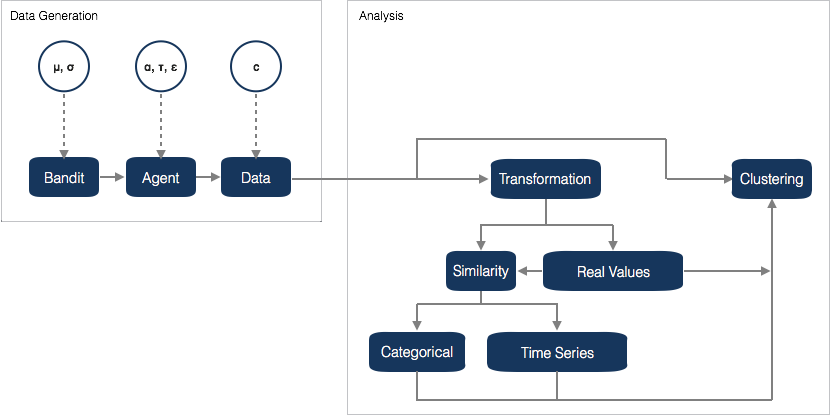
\includegraphics[width=\textwidth]{Pictures/flow01.png}
	\caption{Flowchart experiment desgin}
	\label{fig:flow}
\end{figure}

Concerning our data we find two main challanges. First, our data have a categorical nature. Furhtermore, the learning process also imposes a time series dependence on the data. We address this issue in the following ways. 
The first approach is to map the series of choices to a real valued series. For each time step we can compute \textit{Shannon's Entropy} based on the empirical probability of the choices. Let $X$ be a discrete random variable with probability $p$, then the entropy is defined as:
\begin{flalign}
H(X) := -\sum_{i=1}^{N} p_i \log_2 p_i
\end{flalign}
Entropy gives measure on how random a random variable behaves. Therefore, transforming choices to sequentiel entropy is to discriminate individuals by the randomness

\subsection{Reinforcement Learning backround and multi arm bandits}

\textit{Reinforcement Learning} (RIL) is a branch of \textit{Machine Learning} try model how an artificial agents interact with its environment and learns from the process over time. \\
In particular an agents is confronted with the task of choosing sequently from a set of choices. In comparison to \textit{supervised learning}, where an agent is learning based on set of examples an agent in RIL doesn't have any knowledge about the system apriori. Therefore, it has to learn the nature of the system by sequentially interacting with its environment and keeping tack of the obtained information. Since the agent doesn't have any apriori information about the system it has to explore new possible action and so has to deviate from the optimal action. Furthermore, it has to keep track of value of each action he did so far. So the main task of the agent is to balance exploration and explotation. 
There are to basic approaches to model this trade-off; An \textit{"Epsilon-Greedy"} selection method and Soft \textit{"Softmax"} selection method. Before explaining both cocepts we introduce the value function for a given action $a$. Therefore,  let $Q_t(a)$ be the value function of action defined as:
\begin{flalign}
Q_t(a) := \frac{R_1 + R_2 + \dots + R_{K_\alpha}}{K_\alpha}
\end{flalign}
The value function is the average over rewards. 

Considering now epsilon greedy action selection mehtod: The rule in general is to select the next action as the current current highest value function. However, to model exploration we introduce a random element to deviate from that greedy strategy. Following that the next action
\begin{flalign}
a_{t+1} = \begin{cases} 
\text{random action} & \text{, with probability } \epsilon \\
\arg \max_i Q_t(i) & \text{, with probability } 1-\epsilon
\end{cases}
\end{flalign}
where $\epsilon \in [0,1]$ is a parameter controling the random behaviour of the agent. 

In the softmax action selection method compute for each action a probability (also called \textit{Boltzmann Distribution)}. The probability for action a is computed by:
\begin{flalign}
P(a_{t}|X) = \frac{e^{\frac{Q_t(a)}{\tau}}}{\sum_{i}^{K} e^{\frac{Q_t(i)}{\tau}}}
\end{flalign}
In each iteration the next action of the agent is drawn with probability $p_a$: 
\begin{flalign}
a_{t+1} \sim p_a
\end{flalign}

After selecting an action the agent is updating its believe of the chosen action. Formally the update rule is defined
\begin{flalign}
Q(a)_{k+1} = Q(a)_k + \alpha \left[ R(a)_k -  Q(a)_k	 \right],
\end{flalign}
where $\alpha$ is a is the  non negativ \textit{learning rate} defining how much the current action is affecting the believes.

\subsection{Unsupervised Learning}

We consider several unsupervised clustering techniques. A technical description for all of the is provided in 

\begin{table}[!htb]
	\centering
	\begin{tabular}{|c| c| c |}
		\toprule \toprule
		\textbf{Algorithm} & Input & Datatype  \\
		\hline
		Spectral Clustering & Similarity Matrix & -  \\
		Affinity Propagation & Similarity Matrix & -  \\
		K-Means Clustering & Data Matrix & -  \\
		Ward Clustering & Data Matrix & -  \\
		PCA + 	Ward Clustering   & Data Matrix & -  \\
		\bottomrule
	\end{tabular}
	\caption{Overview clustering algorithms}
\end{table}

\pagebreak	
\subsection{Simmulation results}

The following table shows a snippet of our simmulation results. 
\pagebreak

\begin{sidewaystable}[!h]
	\centering
	\begin{tabular}{| l || c | c | c | c | c | c | c | c | c | c || c  |  c | c | c | c | c | }
		\toprule \toprule
		\textbf{Specification} &$\boldsymbol{\mu}$ & $\boldsymbol{\sigma}$ & \textbf{CL Size} & \textbf{SD} & \textbf{Decision} & $\boldsymbol{\alpha}$  &  $\boldsymbol{\tau}$  & \textbf{N} & \textbf{ALG} & \textbf{TRNS} &  \textbf{MI} & \textbf{NMI} &  \textbf{AMI} &  \textbf{CS} &  \textbf{HS } & \textbf{VMS}     \\
		\hline
		1 & -  & -& -& -& -& -& -& -& -& -& -& -& - & - \\
		\bottomrule
	\end{tabular}
	\caption{Overview Outcome }
\end{sidewaystable}


% Created by tikzDevice version 0.10.1 on 2016-06-03 17:10:08
% !TEX encoding = UTF-8 Unicode
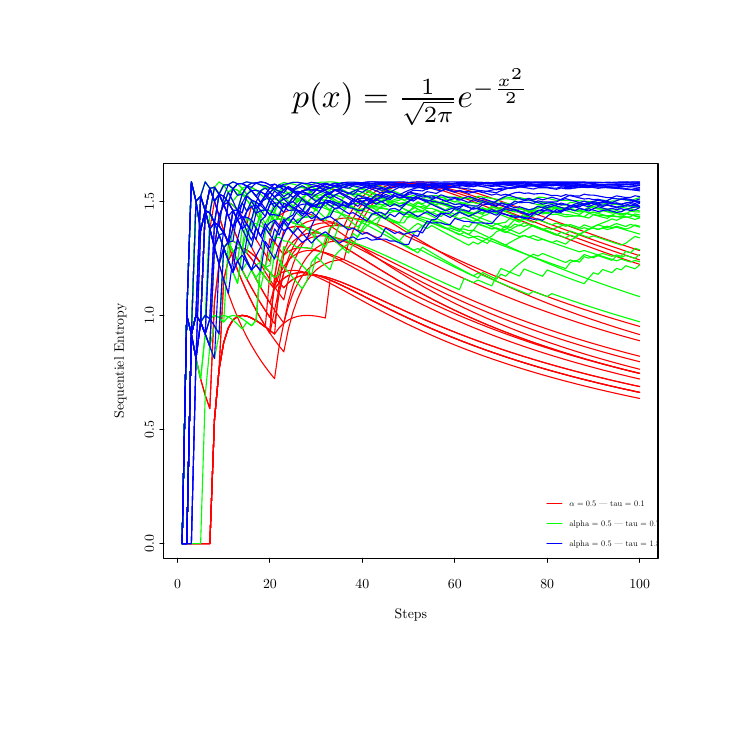
\begin{tikzpicture}[x=1pt,y=1pt]
\definecolor{fillColor}{RGB}{255,255,255}
\path[use as bounding box,fill=fillColor,fill opacity=0.00] (0,0) rectangle (252.94,252.94);
\begin{scope}
\path[clip] ( 49.20, 61.20) rectangle (227.75,203.75);
\definecolor{drawColor}{RGB}{255,0,0}

\path[draw=drawColor,line width= 0.4pt,line join=round,line cap=round] ( 55.81, 66.48) --
	( 57.48, 66.48) --
	( 59.15,142.23) --
	( 60.82,148.97) --
	( 62.49,146.57) --
	( 64.16,186.85) --
	( 65.83,194.89) --
	( 67.50,195.27) --
	( 69.17,192.73) --
	( 70.84,189.02) --
	( 72.51,184.89) --
	( 74.18,180.68) --
	( 75.85,176.58) --
	( 77.52,172.65) --
	( 79.19,168.93) --
	( 80.86,165.42) --
	( 82.53,162.13) --
	( 84.20,159.04) --
	( 85.87,156.15) --
	( 87.54,153.43) --
	( 89.21,150.87) --
	( 90.88,158.71) --
	( 92.55,164.35) --
	( 94.22,168.48) --
	( 95.89,171.51) --
	( 97.56,173.73) --
	( 99.23,175.33) --
	(100.90,176.43) --
	(102.57,177.15) --
	(104.24,177.56) --
	(105.91,177.72) --
	(107.58,177.69) --
	(109.25,177.49) --
	(110.92,177.15) --
	(112.59,176.71) --
	(114.26,176.18) --
	(115.93,175.58) --
	(117.60,174.92) --
	(119.27,174.22) --
	(120.94,173.48) --
	(122.61,172.71) --
	(124.28,171.91) --
	(125.95,171.10) --
	(127.62,170.28) --
	(129.29,169.44) --
	(130.96,168.60) --
	(132.63,167.76) --
	(134.30,166.92) --
	(135.97,166.07) --
	(137.64,165.23) --
	(139.31,164.40) --
	(140.98,163.57) --
	(142.65,162.75) --
	(144.32,161.93) --
	(145.99,161.12) --
	(147.66,160.32) --
	(149.33,159.53) --
	(151.00,158.75) --
	(152.67,157.98) --
	(154.34,157.22) --
	(156.01,156.47) --
	(157.68,155.72) --
	(159.35,154.99) --
	(161.02,154.27) --
	(162.69,153.56) --
	(164.36,152.86) --
	(166.03,152.17) --
	(167.70,151.48) --
	(169.37,150.81) --
	(171.04,150.15) --
	(172.71,149.50) --
	(174.38,148.86) --
	(176.05,148.22) --
	(177.71,147.60) --
	(179.38,146.99) --
	(181.05,146.38) --
	(182.72,145.78) --
	(184.39,145.20) --
	(186.06,144.62) --
	(187.73,144.05) --
	(189.40,143.48) --
	(191.07,142.93) --
	(192.74,142.38) --
	(194.41,141.85) --
	(196.08,141.32) --
	(197.75,140.79) --
	(199.42,140.28) --
	(201.09,139.77) --
	(202.76,139.27) --
	(204.43,138.78) --
	(206.10,138.29) --
	(207.77,137.81) --
	(209.44,137.34) --
	(211.11,136.87) --
	(212.78,136.41) --
	(214.45,135.96) --
	(216.12,135.51) --
	(217.79,135.07) --
	(219.46,134.64) --
	(221.13,134.21);
\end{scope}
\begin{scope}
\path[clip] (  0.00,  0.00) rectangle (252.94,252.94);
\definecolor{drawColor}{RGB}{0,0,0}

\path[draw=drawColor,line width= 0.4pt,line join=round,line cap=round] ( 54.14, 61.20) -- (221.13, 61.20);

\path[draw=drawColor,line width= 0.4pt,line join=round,line cap=round] ( 54.14, 61.20) -- ( 54.14, 59.77);

\path[draw=drawColor,line width= 0.4pt,line join=round,line cap=round] ( 87.54, 61.20) -- ( 87.54, 59.77);

\path[draw=drawColor,line width= 0.4pt,line join=round,line cap=round] (120.94, 61.20) -- (120.94, 59.77);

\path[draw=drawColor,line width= 0.4pt,line join=round,line cap=round] (154.34, 61.20) -- (154.34, 59.77);

\path[draw=drawColor,line width= 0.4pt,line join=round,line cap=round] (187.73, 61.20) -- (187.73, 59.77);

\path[draw=drawColor,line width= 0.4pt,line join=round,line cap=round] (221.13, 61.20) -- (221.13, 59.77);

\node[text=drawColor,anchor=base,inner sep=0pt, outer sep=0pt, scale=  0.50] at ( 54.14, 50.40) {0};

\node[text=drawColor,anchor=base,inner sep=0pt, outer sep=0pt, scale=  0.50] at ( 87.54, 50.40) {20};

\node[text=drawColor,anchor=base,inner sep=0pt, outer sep=0pt, scale=  0.50] at (120.94, 50.40) {40};

\node[text=drawColor,anchor=base,inner sep=0pt, outer sep=0pt, scale=  0.50] at (154.34, 50.40) {60};

\node[text=drawColor,anchor=base,inner sep=0pt, outer sep=0pt, scale=  0.50] at (187.73, 50.40) {80};

\node[text=drawColor,anchor=base,inner sep=0pt, outer sep=0pt, scale=  0.50] at (221.13, 50.40) {100};

\path[draw=drawColor,line width= 0.4pt,line join=round,line cap=round] ( 49.20, 66.48) -- ( 49.20,190.22);

\path[draw=drawColor,line width= 0.4pt,line join=round,line cap=round] ( 49.20, 66.48) -- ( 47.77, 66.48);

\path[draw=drawColor,line width= 0.4pt,line join=round,line cap=round] ( 49.20,107.73) -- ( 47.77,107.73);

\path[draw=drawColor,line width= 0.4pt,line join=round,line cap=round] ( 49.20,148.97) -- ( 47.77,148.97);

\path[draw=drawColor,line width= 0.4pt,line join=round,line cap=round] ( 49.20,190.22) -- ( 47.77,190.22);

\node[text=drawColor,rotate= 90.00,anchor=base,inner sep=0pt, outer sep=0pt, scale=  0.50] at ( 45.60, 66.48) {0.0};

\node[text=drawColor,rotate= 90.00,anchor=base,inner sep=0pt, outer sep=0pt, scale=  0.50] at ( 45.60,107.73) {0.5};

\node[text=drawColor,rotate= 90.00,anchor=base,inner sep=0pt, outer sep=0pt, scale=  0.50] at ( 45.60,148.97) {1.0};

\node[text=drawColor,rotate= 90.00,anchor=base,inner sep=0pt, outer sep=0pt, scale=  0.50] at ( 45.60,190.22) {1.5};

\path[draw=drawColor,line width= 0.4pt,line join=round,line cap=round] ( 49.20, 61.20) --
	(227.75, 61.20) --
	(227.75,203.75) --
	( 49.20,203.75) --
	( 49.20, 61.20);
\end{scope}
\begin{scope}
\path[clip] (  0.00,  0.00) rectangle (252.94,252.94);
\definecolor{drawColor}{RGB}{0,0,0}

\node[text=drawColor,anchor=base,inner sep=0pt, outer sep=0pt, scale=  0.50] at (138.47, 39.60) {Steps};

\node[text=drawColor,rotate= 90.00,anchor=base,inner sep=0pt, outer sep=0pt, scale=  0.50] at ( 34.80,132.47) {Sequentiel Entropy};
\end{scope}
\begin{scope}
\path[clip] ( 49.20, 61.20) rectangle (227.75,203.75);
\definecolor{drawColor}{RGB}{255,0,0}

\path[draw=drawColor,line width= 0.4pt,line join=round,line cap=round] ( 55.81, 66.48) --
	( 57.48, 66.48) --
	( 59.15,142.23) --
	( 60.82,148.97) --
	( 62.49,146.57) --
	( 64.16,142.23) --
	( 65.83,137.68) --
	( 67.50,173.62) --
	( 69.17,184.90) --
	( 70.84,189.02) --
	( 72.51,189.80) --
	( 74.18,188.84) --
	( 75.85,186.96) --
	( 77.52,184.57) --
	( 79.19,181.93) --
	( 80.86,188.34) --
	( 82.53,185.82) --
	( 84.20,183.23) --
	( 85.87,180.63) --
	( 87.54,178.07) --
	( 89.21,182.79) --
	( 90.88,184.89) --
	( 92.55,186.17) --
	( 94.22,186.85) --
	( 95.89,187.07) --
	( 97.56,186.96) --
	( 99.23,186.58) --
	(100.90,185.99) --
	(102.57,185.26) --
	(104.24,184.40) --
	(105.91,183.45) --
	(107.58,182.43) --
	(109.25,181.36) --
	(110.92,180.26) --
	(112.59,179.13) --
	(114.26,177.98) --
	(115.93,176.82) --
	(117.60,175.66) --
	(119.27,174.50) --
	(120.94,173.34) --
	(122.61,172.20) --
	(124.28,171.06) --
	(125.95,169.93) --
	(127.62,168.82) --
	(129.29,167.73) --
	(130.96,166.65) --
	(132.63,165.58) --
	(134.30,164.54) --
	(135.97,163.51) --
	(137.64,162.50) --
	(139.31,161.50) --
	(140.98,160.53) --
	(142.65,159.57) --
	(144.32,158.63) --
	(145.99,157.71) --
	(147.66,156.80) --
	(149.33,155.91) --
	(151.00,155.04) --
	(152.67,154.18) --
	(154.34,153.34) --
	(156.01,152.52) --
	(157.68,151.71) --
	(159.35,150.91) --
	(161.02,150.13) --
	(162.69,149.37) --
	(164.36,148.62) --
	(166.03,147.88) --
	(167.70,147.16) --
	(169.37,146.45) --
	(171.04,145.75) --
	(172.71,145.06) --
	(174.38,144.39) --
	(176.05,143.73) --
	(177.71,143.08) --
	(179.38,142.44) --
	(181.05,141.82) --
	(182.72,141.20) --
	(184.39,140.60) --
	(186.06,140.00) --
	(187.73,139.42) --
	(189.40,138.84) --
	(191.07,138.28) --
	(192.74,137.72) --
	(194.41,137.17) --
	(196.08,136.64) --
	(197.75,136.11) --
	(199.42,135.59) --
	(201.09,135.07) --
	(202.76,134.57) --
	(204.43,134.07) --
	(206.10,133.59) --
	(207.77,133.11) --
	(209.44,132.63) --
	(211.11,132.17) --
	(212.78,131.71) --
	(214.45,131.25) --
	(216.12,130.81) --
	(217.79,130.37) --
	(219.46,129.94) --
	(221.13,129.51);

\path[draw=drawColor,line width= 0.4pt,line join=round,line cap=round] ( 55.81, 66.48) --
	( 57.48,148.97) --
	( 59.15,142.23) --
	( 60.82,133.40) --
	( 62.49,126.03) --
	( 64.16,120.10) --
	( 65.83,115.29) --
	( 67.50,154.03) --
	( 69.17,167.48) --
	( 70.84,173.34) --
	( 72.51,175.55) --
	( 74.18,175.78) --
	( 75.85,174.90) --
	( 77.52,173.37) --
	( 79.19,171.48) --
	( 80.86,169.39) --
	( 82.53,167.21) --
	( 84.20,164.99) --
	( 85.87,162.78) --
	( 87.54,160.61) --
	( 89.21,158.50) --
	( 90.88,160.79) --
	( 92.55,162.38) --
	( 94.22,163.43) --
	( 95.89,164.06) --
	( 97.56,164.37) --
	( 99.23,164.43) --
	(100.90,164.28) --
	(102.57,163.98) --
	(104.24,163.55) --
	(105.91,163.01) --
	(107.58,162.40) --
	(109.25,161.73) --
	(110.92,161.01) --
	(112.59,160.24) --
	(114.26,159.46) --
	(115.93,158.65) --
	(117.60,157.82) --
	(119.27,156.98) --
	(120.94,156.14) --
	(122.61,155.30) --
	(124.28,154.46) --
	(125.95,153.61) --
	(127.62,152.78) --
	(129.29,151.95) --
	(130.96,151.12) --
	(132.63,150.31) --
	(134.30,149.50) --
	(135.97,148.71) --
	(137.64,147.92) --
	(139.31,147.15) --
	(140.98,146.39) --
	(142.65,145.63) --
	(144.32,144.89) --
	(145.99,144.16) --
	(147.66,143.45) --
	(149.33,142.74) --
	(151.00,142.05) --
	(152.67,141.36) --
	(154.34,140.69) --
	(156.01,140.03) --
	(157.68,139.38) --
	(159.35,138.74) --
	(161.02,138.11) --
	(162.69,137.50) --
	(164.36,136.89) --
	(166.03,136.29) --
	(167.70,135.71) --
	(169.37,135.13) --
	(171.04,134.56) --
	(172.71,134.00) --
	(174.38,133.45) --
	(176.05,132.91) --
	(177.71,132.38) --
	(179.38,131.86) --
	(181.05,131.35) --
	(182.72,130.84) --
	(184.39,130.35) --
	(186.06,129.86) --
	(187.73,129.38) --
	(189.40,128.90) --
	(191.07,128.44) --
	(192.74,127.98) --
	(194.41,127.53) --
	(196.08,127.08) --
	(197.75,126.64) --
	(199.42,126.21) --
	(201.09,125.79) --
	(202.76,125.37) --
	(204.43,124.96) --
	(206.10,124.55) --
	(207.77,124.15) --
	(209.44,123.76) --
	(211.11,123.37) --
	(212.78,122.99) --
	(214.45,122.61) --
	(216.12,122.24) --
	(217.79,121.88) --
	(219.46,121.51) --
	(221.13,121.16);

\path[draw=drawColor,line width= 0.4pt,line join=round,line cap=round] ( 55.81, 66.48) --
	( 57.48, 66.48) --
	( 59.15,142.23) --
	( 60.82,148.97) --
	( 62.49,146.57) --
	( 64.16,186.85) --
	( 65.83,194.89) --
	( 67.50,190.22) --
	( 69.17,184.90) --
	( 70.84,179.57) --
	( 72.51,174.49) --
	( 74.18,169.73) --
	( 75.85,165.32) --
	( 77.52,161.25) --
	( 79.19,157.49) --
	( 80.86,154.03) --
	( 82.53,150.82) --
	( 84.20,147.85) --
	( 85.87,145.09) --
	( 87.54,142.53) --
	( 89.21,140.14) --
	( 90.88,137.91) --
	( 92.55,135.81) --
	( 94.22,144.07) --
	( 95.89,150.24) --
	( 97.56,154.97) --
	( 99.23,158.63) --
	(100.90,161.47) --
	(102.57,163.68) --
	(104.24,165.38) --
	(105.91,166.67) --
	(107.58,167.62) --
	(109.25,168.31) --
	(110.92,168.76) --
	(112.59,169.03) --
	(114.26,169.14) --
	(115.93,175.01) --
	(117.60,179.60) --
	(119.27,183.25) --
	(120.94,186.20) --
	(122.61,188.60) --
	(124.28,190.54) --
	(125.95,192.11) --
	(127.62,193.37) --
	(129.29,194.37) --
	(130.96,195.15) --
	(132.63,195.74) --
	(134.30,196.16) --
	(135.97,196.45) --
	(137.64,196.62) --
	(139.31,196.67) --
	(140.98,196.64) --
	(142.65,196.53) --
	(144.32,196.34) --
	(145.99,196.10) --
	(147.66,195.80) --
	(149.33,195.45) --
	(151.00,195.07) --
	(152.67,194.64) --
	(154.34,194.19) --
	(156.01,193.70) --
	(157.68,193.20) --
	(159.35,192.67) --
	(161.02,192.12) --
	(162.69,191.56) --
	(164.36,190.99) --
	(166.03,190.40) --
	(167.70,189.80) --
	(169.37,189.20) --
	(171.04,188.59) --
	(172.71,187.97) --
	(174.38,187.35) --
	(176.05,186.73) --
	(177.71,186.10) --
	(179.38,185.47) --
	(181.05,184.84) --
	(182.72,184.22) --
	(184.39,183.59) --
	(186.06,182.96) --
	(187.73,182.33) --
	(189.40,181.71) --
	(191.07,181.09) --
	(192.74,180.47) --
	(194.41,179.85) --
	(196.08,179.24) --
	(197.75,178.63) --
	(199.42,178.03) --
	(201.09,177.42) --
	(202.76,176.82) --
	(204.43,176.23) --
	(206.10,175.64) --
	(207.77,175.05) --
	(209.44,174.47) --
	(211.11,173.90) --
	(212.78,173.33) --
	(214.45,172.76) --
	(216.12,172.19) --
	(217.79,171.64) --
	(219.46,171.08) --
	(221.13,170.54);

\path[draw=drawColor,line width= 0.4pt,line join=round,line cap=round] ( 55.81, 66.48) --
	( 57.48, 66.48) --
	( 59.15, 66.48) --
	( 60.82, 66.48) --
	( 62.49, 66.48) --
	( 64.16, 66.48) --
	( 65.83, 66.48) --
	( 67.50,111.32) --
	( 69.17,129.52) --
	( 70.84,139.18) --
	( 72.51,144.49) --
	( 74.18,147.31) --
	( 75.85,148.62) --
	( 77.52,148.97) --
	( 79.19,148.71) --
	( 80.86,148.04) --
	( 82.53,147.11) --
	( 84.20,146.01) --
	( 85.87,144.80) --
	( 87.54,164.51) --
	( 89.21,162.65) --
	( 90.88,163.98) --
	( 92.55,164.78) --
	( 94.22,165.17) --
	( 95.89,165.26) --
	( 97.56,165.11) --
	( 99.23,164.77) --
	(100.90,164.28) --
	(102.57,163.68) --
	(104.24,163.00) --
	(105.91,162.24) --
	(107.58,161.44) --
	(109.25,160.59) --
	(110.92,159.72) --
	(112.59,158.82) --
	(114.26,157.92) --
	(115.93,157.00) --
	(117.60,156.08) --
	(119.27,155.17) --
	(120.94,154.25) --
	(122.61,153.34) --
	(124.28,152.44) --
	(125.95,151.55) --
	(127.62,150.66) --
	(129.29,149.79) --
	(130.96,148.93) --
	(132.63,148.08) --
	(134.30,147.25) --
	(135.97,146.43) --
	(137.64,145.62) --
	(139.31,144.83) --
	(140.98,144.05) --
	(142.65,143.28) --
	(144.32,142.53) --
	(145.99,141.79) --
	(147.66,141.06) --
	(149.33,140.34) --
	(151.00,139.64) --
	(152.67,138.96) --
	(154.34,138.28) --
	(156.01,137.62) --
	(157.68,136.96) --
	(159.35,136.32) --
	(161.02,135.70) --
	(162.69,135.08) --
	(164.36,134.47) --
	(166.03,133.88) --
	(167.70,133.29) --
	(169.37,132.72) --
	(171.04,132.16) --
	(172.71,131.60) --
	(174.38,131.06) --
	(176.05,130.52) --
	(177.71,130.00) --
	(179.38,129.48) --
	(181.05,128.97) --
	(182.72,128.47) --
	(184.39,127.98) --
	(186.06,127.50) --
	(187.73,127.03) --
	(189.40,126.56) --
	(191.07,126.10) --
	(192.74,125.65) --
	(194.41,125.20) --
	(196.08,124.77) --
	(197.75,124.34) --
	(199.42,123.91) --
	(201.09,123.50) --
	(202.76,123.09) --
	(204.43,122.68) --
	(206.10,122.28) --
	(207.77,121.89) --
	(209.44,121.51) --
	(211.11,121.13) --
	(212.78,120.75) --
	(214.45,120.38) --
	(216.12,120.02) --
	(217.79,119.66) --
	(219.46,119.31) --
	(221.13,118.96);

\path[draw=drawColor,line width= 0.4pt,line join=round,line cap=round] ( 55.81, 66.48) --
	( 57.48, 66.48) --
	( 59.15, 66.48) --
	( 60.82, 66.48) --
	( 62.49, 66.48) --
	( 64.16, 66.48) --
	( 65.83, 66.48) --
	( 67.50,111.32) --
	( 69.17,129.52) --
	( 70.84,139.18) --
	( 72.51,144.49) --
	( 74.18,147.31) --
	( 75.85,148.62) --
	( 77.52,148.97) --
	( 79.19,148.71) --
	( 80.86,148.04) --
	( 82.53,147.11) --
	( 84.20,146.01) --
	( 85.87,144.80) --
	( 87.54,143.53) --
	( 89.21,162.65) --
	( 90.88,160.79) --
	( 92.55,158.97) --
	( 94.22,160.78) --
	( 95.89,162.05) --
	( 97.56,162.90) --
	( 99.23,163.41) --
	(100.90,163.65) --
	(102.57,163.68) --
	(104.24,163.55) --
	(105.91,163.27) --
	(107.58,162.88) --
	(109.25,162.41) --
	(110.92,161.86) --
	(112.59,161.25) --
	(114.26,160.60) --
	(115.93,159.91) --
	(117.60,159.20) --
	(119.27,158.46) --
	(120.94,157.70) --
	(122.61,156.94) --
	(124.28,156.16) --
	(125.95,155.39) --
	(127.62,154.61) --
	(129.29,153.83) --
	(130.96,153.05) --
	(132.63,152.27) --
	(134.30,151.51) --
	(135.97,150.74) --
	(137.64,149.99) --
	(139.31,149.24) --
	(140.98,148.50) --
	(142.65,147.77) --
	(144.32,147.04) --
	(145.99,146.33) --
	(147.66,145.63) --
	(149.33,144.94) --
	(151.00,144.25) --
	(152.67,143.58) --
	(154.34,142.91) --
	(156.01,142.26) --
	(157.68,141.62) --
	(159.35,140.98) --
	(161.02,140.36) --
	(162.69,139.74) --
	(164.36,139.14) --
	(166.03,138.54) --
	(167.70,137.96) --
	(169.37,137.38) --
	(171.04,136.81) --
	(172.71,136.25) --
	(174.38,135.70) --
	(176.05,135.16) --
	(177.71,134.63) --
	(179.38,134.10) --
	(181.05,133.59) --
	(182.72,133.08) --
	(184.39,132.58) --
	(186.06,132.08) --
	(187.73,131.60) --
	(189.40,131.12) --
	(191.07,130.65) --
	(192.74,130.18) --
	(194.41,129.73) --
	(196.08,129.28) --
	(197.75,128.83) --
	(199.42,128.40) --
	(201.09,127.97) --
	(202.76,127.54) --
	(204.43,127.12) --
	(206.10,126.71) --
	(207.77,126.31) --
	(209.44,125.90) --
	(211.11,125.51) --
	(212.78,125.12) --
	(214.45,124.74) --
	(216.12,124.36) --
	(217.79,123.99) --
	(219.46,123.62) --
	(221.13,123.26);

\path[draw=drawColor,line width= 0.4pt,line join=round,line cap=round] ( 55.81, 66.48) --
	( 57.48, 66.48) --
	( 59.15,142.23) --
	( 60.82,190.22) --
	( 62.49,192.03) --
	( 64.16,186.85) --
	( 65.83,180.22) --
	( 67.50,182.43) --
	( 69.17,181.32) --
	( 70.84,178.75) --
	( 72.51,175.55) --
	( 74.18,172.12) --
	( 75.85,168.68) --
	( 77.52,165.31) --
	( 79.19,162.08) --
	( 80.86,159.01) --
	( 82.53,156.09) --
	( 84.20,153.34) --
	( 85.87,150.74) --
	( 87.54,148.29) --
	( 89.21,145.98) --
	( 90.88,156.87) --
	( 92.55,164.35) --
	( 94.22,169.73) --
	( 95.89,173.67) --
	( 97.56,176.58) --
	( 99.23,178.70) --
	(100.90,180.22) --
	(102.57,181.26) --
	(104.24,181.93) --
	(105.91,182.30) --
	(107.58,182.43) --
	(109.25,182.37) --
	(110.92,182.14) --
	(112.59,181.78) --
	(114.26,181.32) --
	(115.93,180.77) --
	(117.60,180.33) --
	(119.27,179.82) --
	(120.94,183.46) --
	(122.61,186.40) --
	(124.28,188.80) --
	(125.95,190.76) --
	(127.62,192.35) --
	(129.29,193.64) --
	(130.96,194.67) --
	(132.63,195.48) --
	(134.30,196.11) --
	(135.97,196.57) --
	(137.64,196.89) --
	(139.31,197.09) --
	(140.98,197.18) --
	(142.65,197.18) --
	(144.32,197.10) --
	(145.99,196.95) --
	(147.66,196.74) --
	(149.33,196.47) --
	(151.00,196.16) --
	(152.67,195.80) --
	(154.34,195.40) --
	(156.01,194.97) --
	(157.68,194.52) --
	(159.35,194.04) --
	(161.02,193.53) --
	(162.69,193.01) --
	(164.36,192.47) --
	(166.03,191.92) --
	(167.70,191.35) --
	(169.37,190.78) --
	(171.04,190.19) --
	(172.71,189.60) --
	(174.38,189.00) --
	(176.05,188.40) --
	(177.71,187.79) --
	(179.38,187.18) --
	(181.05,186.57) --
	(182.72,185.95) --
	(184.39,185.34) --
	(186.06,184.72) --
	(187.73,184.11) --
	(189.40,183.49) --
	(191.07,182.88) --
	(192.74,182.27) --
	(194.41,181.66) --
	(196.08,181.05) --
	(197.75,180.45) --
	(199.42,179.85) --
	(201.09,179.25) --
	(202.76,178.66) --
	(204.43,178.07) --
	(206.10,177.48) --
	(207.77,176.90) --
	(209.44,176.32) --
	(211.11,175.75) --
	(212.78,175.17) --
	(214.45,174.61) --
	(216.12,174.05) --
	(217.79,173.49) --
	(219.46,172.94) --
	(221.13,172.39);

\path[draw=drawColor,line width= 0.4pt,line join=round,line cap=round] ( 55.81, 66.48) --
	( 57.48, 66.48) --
	( 59.15, 66.48) --
	( 60.82, 66.48) --
	( 62.49, 66.48) --
	( 64.16, 66.48) --
	( 65.83, 66.48) --
	( 67.50,111.32) --
	( 69.17,129.52) --
	( 70.84,139.18) --
	( 72.51,144.49) --
	( 74.18,147.31) --
	( 75.85,148.62) --
	( 77.52,148.97) --
	( 79.19,148.71) --
	( 80.86,148.04) --
	( 82.53,147.11) --
	( 84.20,168.16) --
	( 85.87,166.36) --
	( 87.54,176.74) --
	( 89.21,174.77) --
	( 90.88,181.52) --
	( 92.55,186.17) --
	( 94.22,189.39) --
	( 95.89,191.59) --
	( 97.56,193.04) --
	( 99.23,193.92) --
	(100.90,194.89) --
	(102.57,195.43) --
	(104.24,195.63) --
	(105.91,195.56) --
	(107.58,195.27) --
	(109.25,194.82) --
	(110.92,194.22) --
	(112.59,193.52) --
	(114.26,192.73) --
	(115.93,191.87) --
	(117.60,190.96) --
	(119.27,190.01) --
	(120.94,189.02) --
	(122.61,188.01) --
	(124.28,186.98) --
	(125.95,185.93) --
	(127.62,184.89) --
	(129.29,183.83) --
	(130.96,182.78) --
	(132.63,181.73) --
	(134.30,180.68) --
	(135.97,179.64) --
	(137.64,178.61) --
	(139.31,177.59) --
	(140.98,176.58) --
	(142.65,175.58) --
	(144.32,174.59) --
	(145.99,173.61) --
	(147.66,172.65) --
	(149.33,171.70) --
	(151.00,170.76) --
	(152.67,169.84) --
	(154.34,168.93) --
	(156.01,168.03) --
	(157.68,167.15) --
	(159.35,166.28) --
	(161.02,165.42) --
	(162.69,164.58) --
	(164.36,163.75) --
	(166.03,162.94) --
	(167.70,162.13) --
	(169.37,161.34) --
	(171.04,160.56) --
	(172.71,159.80) --
	(174.38,159.04) --
	(176.05,158.30) --
	(177.71,157.57) --
	(179.38,156.85) --
	(181.05,156.15) --
	(182.72,155.45) --
	(184.39,154.77) --
	(186.06,154.09) --
	(187.73,153.43) --
	(189.40,152.77) --
	(191.07,152.13) --
	(192.74,151.50) --
	(194.41,150.87) --
	(196.08,150.26) --
	(197.75,149.65) --
	(199.42,149.05) --
	(201.09,148.47) --
	(202.76,147.89) --
	(204.43,147.32) --
	(206.10,146.76) --
	(207.77,146.20) --
	(209.44,145.66) --
	(211.11,145.12) --
	(212.78,144.59) --
	(214.45,144.07) --
	(216.12,143.55) --
	(217.79,143.05) --
	(219.46,142.54) --
	(221.13,142.05);

\path[draw=drawColor,line width= 0.4pt,line join=round,line cap=round] ( 55.81, 66.48) --
	( 57.48, 66.48) --
	( 59.15,142.23) --
	( 60.82,190.22) --
	( 62.49,192.03) --
	( 64.16,186.85) --
	( 65.83,180.22) --
	( 67.50,182.43) --
	( 69.17,181.32) --
	( 70.84,178.75) --
	( 72.51,175.55) --
	( 74.18,172.12) --
	( 75.85,168.68) --
	( 77.52,165.31) --
	( 79.19,162.08) --
	( 80.86,159.01) --
	( 82.53,156.09) --
	( 84.20,153.34) --
	( 85.87,150.74) --
	( 87.54,148.29) --
	( 89.21,159.32) --
	( 90.88,163.57) --
	( 92.55,166.65) --
	( 94.22,168.85) --
	( 95.89,170.40) --
	( 97.56,171.43) --
	( 99.23,172.07) --
	(100.90,172.39) --
	(102.57,172.46) --
	(104.24,172.34) --
	(105.91,172.05) --
	(107.58,171.64) --
	(109.25,171.12) --
	(110.92,170.52) --
	(112.59,169.86) --
	(114.26,169.14) --
	(115.93,168.38) --
	(117.60,167.59) --
	(119.27,166.78) --
	(120.94,165.95) --
	(122.61,165.10) --
	(124.28,164.25) --
	(125.95,163.39) --
	(127.62,162.52) --
	(129.29,161.66) --
	(130.96,160.80) --
	(132.63,159.95) --
	(134.30,159.10) --
	(135.97,158.26) --
	(137.64,157.43) --
	(139.31,156.60) --
	(140.98,155.78) --
	(142.65,154.98) --
	(144.32,154.18) --
	(145.99,153.40) --
	(147.66,152.62) --
	(149.33,151.86) --
	(151.00,151.10) --
	(152.67,150.36) --
	(154.34,149.63) --
	(156.01,148.91) --
	(157.68,148.20) --
	(159.35,147.51) --
	(161.02,146.82) --
	(162.69,146.14) --
	(164.36,145.48) --
	(166.03,144.82) --
	(167.70,144.18) --
	(169.37,143.55) --
	(171.04,142.92) --
	(172.71,142.31) --
	(174.38,141.70) --
	(176.05,141.11) --
	(177.71,140.52) --
	(179.38,139.95) --
	(181.05,139.38) --
	(182.72,138.82) --
	(184.39,138.27) --
	(186.06,137.73) --
	(187.73,137.20) --
	(189.40,136.67) --
	(191.07,136.16) --
	(192.74,135.65) --
	(194.41,135.15) --
	(196.08,134.65) --
	(197.75,134.17) --
	(199.42,133.69) --
	(201.09,133.22) --
	(202.76,132.75) --
	(204.43,132.29) --
	(206.10,131.84) --
	(207.77,131.40) --
	(209.44,130.96) --
	(211.11,130.53) --
	(212.78,130.10) --
	(214.45,129.68) --
	(216.12,129.27) --
	(217.79,128.86) --
	(219.46,128.46) --
	(221.13,128.06);

\path[draw=drawColor,line width= 0.4pt,line join=round,line cap=round] ( 55.81, 66.48) --
	( 57.48, 66.48) --
	( 59.15, 66.48) --
	( 60.82, 66.48) --
	( 62.49, 66.48) --
	( 64.16, 66.48) --
	( 65.83, 66.48) --
	( 67.50,111.32) --
	( 69.17,129.52) --
	( 70.84,139.18) --
	( 72.51,144.49) --
	( 74.18,147.31) --
	( 75.85,148.62) --
	( 77.52,148.97) --
	( 79.19,148.71) --
	( 80.86,148.04) --
	( 82.53,147.11) --
	( 84.20,146.01) --
	( 85.87,144.80) --
	( 87.54,143.53) --
	( 89.21,162.65) --
	( 90.88,160.79) --
	( 92.55,158.97) --
	( 94.22,160.78) --
	( 95.89,162.05) --
	( 97.56,162.90) --
	( 99.23,163.41) --
	(100.90,163.65) --
	(102.57,163.68) --
	(104.24,163.55) --
	(105.91,163.27) --
	(107.58,162.88) --
	(109.25,162.41) --
	(110.92,161.86) --
	(112.59,161.25) --
	(114.26,160.60) --
	(115.93,159.91) --
	(117.60,159.20) --
	(119.27,158.46) --
	(120.94,157.70) --
	(122.61,156.94) --
	(124.28,156.16) --
	(125.95,155.39) --
	(127.62,154.61) --
	(129.29,153.83) --
	(130.96,153.05) --
	(132.63,152.27) --
	(134.30,151.51) --
	(135.97,150.74) --
	(137.64,149.99) --
	(139.31,149.24) --
	(140.98,148.50) --
	(142.65,147.77) --
	(144.32,147.04) --
	(145.99,146.33) --
	(147.66,145.63) --
	(149.33,144.94) --
	(151.00,144.25) --
	(152.67,143.58) --
	(154.34,142.91) --
	(156.01,142.26) --
	(157.68,141.62) --
	(159.35,140.98) --
	(161.02,140.36) --
	(162.69,139.74) --
	(164.36,139.14) --
	(166.03,138.54) --
	(167.70,137.96) --
	(169.37,137.38) --
	(171.04,136.81) --
	(172.71,136.25) --
	(174.38,135.70) --
	(176.05,135.16) --
	(177.71,134.63) --
	(179.38,134.10) --
	(181.05,133.59) --
	(182.72,133.08) --
	(184.39,132.58) --
	(186.06,132.08) --
	(187.73,131.60) --
	(189.40,131.12) --
	(191.07,130.65) --
	(192.74,130.18) --
	(194.41,129.73) --
	(196.08,129.28) --
	(197.75,128.83) --
	(199.42,128.40) --
	(201.09,127.97) --
	(202.76,127.54) --
	(204.43,127.12) --
	(206.10,126.71) --
	(207.77,126.31) --
	(209.44,125.90) --
	(211.11,125.51) --
	(212.78,125.12) --
	(214.45,124.74) --
	(216.12,124.36) --
	(217.79,123.99) --
	(219.46,123.62) --
	(221.13,123.26);

\path[draw=drawColor,line width= 0.4pt,line join=round,line cap=round] ( 55.81, 66.48) --
	( 57.48, 66.48) --
	( 59.15,142.23) --
	( 60.82,148.97) --
	( 62.49,192.03) --
	( 64.16,186.85) --
	( 65.83,180.22) --
	( 67.50,173.62) --
	( 69.17,167.48) --
	( 70.84,161.90) --
	( 72.51,156.87) --
	( 74.18,152.34) --
	( 75.85,148.25) --
	( 77.52,144.55) --
	( 79.19,141.18) --
	( 80.86,138.11) --
	( 82.53,135.31) --
	( 84.20,132.73) --
	( 85.87,130.35) --
	( 87.54,128.15) --
	( 89.21,126.11) --
	( 90.88,137.91) --
	( 92.55,146.20) --
	( 94.22,152.34) --
	( 95.89,156.98) --
	( 97.56,160.53) --
	( 99.23,163.24) --
	(100.90,165.31) --
	(102.57,166.87) --
	(104.24,168.02) --
	(105.91,168.84) --
	(107.58,175.09) --
	(109.25,179.85) --
	(110.92,183.55) --
	(112.59,183.94) --
	(114.26,184.13) --
	(115.93,184.15) --
	(117.60,184.03) --
	(119.27,183.79) --
	(120.94,183.46) --
	(122.61,183.04) --
	(124.28,182.55) --
	(125.95,182.01) --
	(127.62,181.42) --
	(129.29,180.79) --
	(130.96,180.13) --
	(132.63,179.44) --
	(134.30,178.73) --
	(135.97,178.00) --
	(137.64,177.25) --
	(139.31,176.50) --
	(140.98,175.74) --
	(142.65,174.97) --
	(144.32,174.20) --
	(145.99,173.43) --
	(147.66,172.66) --
	(149.33,171.88) --
	(151.00,171.11) --
	(152.67,170.35) --
	(154.34,169.59) --
	(156.01,168.83) --
	(157.68,168.08) --
	(159.35,167.33) --
	(161.02,166.59) --
	(162.69,165.86) --
	(164.36,165.13) --
	(166.03,164.42) --
	(167.70,163.70) --
	(169.37,163.00) --
	(171.04,162.31) --
	(172.71,161.62) --
	(174.38,160.94) --
	(176.05,160.27) --
	(177.71,159.60) --
	(179.38,158.95) --
	(181.05,158.30) --
	(182.72,157.66) --
	(184.39,157.03) --
	(186.06,156.40) --
	(187.73,155.79) --
	(189.40,155.18) --
	(191.07,154.58) --
	(192.74,153.99) --
	(194.41,153.40) --
	(196.08,152.82) --
	(197.75,152.25) --
	(199.42,151.69) --
	(201.09,151.13) --
	(202.76,150.59) --
	(204.43,150.04) --
	(206.10,149.51) --
	(207.77,148.98) --
	(209.44,148.46) --
	(211.11,147.94) --
	(212.78,147.44) --
	(214.45,146.94) --
	(216.12,146.44) --
	(217.79,145.95) --
	(219.46,145.47) --
	(221.13,144.99);

\path[draw=drawColor,line width= 0.4pt,line join=round,line cap=round] ( 55.81, 66.48) --
	( 57.48,148.97) --
	( 59.15,142.23) --
	( 60.82,133.40) --
	( 62.49,126.03) --
	( 64.16,120.10) --
	( 65.83,115.29) --
	( 67.50,154.03) --
	( 69.17,167.48) --
	( 70.84,173.34) --
	( 72.51,175.55) --
	( 74.18,175.78) --
	( 75.85,174.90) --
	( 77.52,173.37) --
	( 79.19,171.48) --
	( 80.86,169.39) --
	( 82.53,167.21) --
	( 84.20,164.99) --
	( 85.87,162.78) --
	( 87.54,160.61) --
	( 89.21,158.50) --
	( 90.88,160.79) --
	( 92.55,162.38) --
	( 94.22,163.43) --
	( 95.89,164.06) --
	( 97.56,164.37) --
	( 99.23,164.43) --
	(100.90,164.28) --
	(102.57,163.98) --
	(104.24,163.55) --
	(105.91,163.01) --
	(107.58,162.40) --
	(109.25,161.73) --
	(110.92,161.01) --
	(112.59,160.24) --
	(114.26,159.46) --
	(115.93,158.65) --
	(117.60,157.82) --
	(119.27,156.98) --
	(120.94,156.14) --
	(122.61,155.30) --
	(124.28,154.46) --
	(125.95,153.61) --
	(127.62,152.78) --
	(129.29,151.95) --
	(130.96,151.12) --
	(132.63,150.31) --
	(134.30,149.50) --
	(135.97,148.71) --
	(137.64,147.92) --
	(139.31,147.15) --
	(140.98,146.39) --
	(142.65,145.63) --
	(144.32,144.89) --
	(145.99,144.16) --
	(147.66,143.45) --
	(149.33,142.74) --
	(151.00,142.05) --
	(152.67,141.36) --
	(154.34,140.69) --
	(156.01,140.03) --
	(157.68,139.38) --
	(159.35,138.74) --
	(161.02,138.11) --
	(162.69,137.50) --
	(164.36,136.89) --
	(166.03,136.29) --
	(167.70,135.71) --
	(169.37,135.13) --
	(171.04,134.56) --
	(172.71,134.00) --
	(174.38,133.45) --
	(176.05,132.91) --
	(177.71,132.38) --
	(179.38,131.86) --
	(181.05,131.35) --
	(182.72,130.84) --
	(184.39,130.35) --
	(186.06,129.86) --
	(187.73,129.38) --
	(189.40,128.90) --
	(191.07,128.44) --
	(192.74,127.98) --
	(194.41,127.53) --
	(196.08,127.08) --
	(197.75,126.64) --
	(199.42,126.21) --
	(201.09,125.79) --
	(202.76,125.37) --
	(204.43,124.96) --
	(206.10,124.55) --
	(207.77,124.15) --
	(209.44,123.76) --
	(211.11,123.37) --
	(212.78,122.99) --
	(214.45,122.61) --
	(216.12,122.24) --
	(217.79,121.88) --
	(219.46,121.51) --
	(221.13,121.16);

\path[draw=drawColor,line width= 0.4pt,line join=round,line cap=round] ( 55.81, 66.48) --
	( 57.48, 66.48) --
	( 59.15, 66.48) --
	( 60.82, 66.48) --
	( 62.49, 66.48) --
	( 64.16, 66.48) --
	( 65.83, 66.48) --
	( 67.50,111.32) --
	( 69.17,129.52) --
	( 70.84,139.18) --
	( 72.51,144.49) --
	( 74.18,147.31) --
	( 75.85,148.62) --
	( 77.52,148.97) --
	( 79.19,148.71) --
	( 80.86,148.04) --
	( 82.53,147.11) --
	( 84.20,146.01) --
	( 85.87,144.80) --
	( 87.54,143.53) --
	( 89.21,142.23) --
	( 90.88,160.79) --
	( 92.55,170.80) --
	( 94.22,172.12) --
	( 95.89,172.94) --
	( 97.56,173.37) --
	( 99.23,173.49) --
	(100.90,173.37) --
	(102.57,173.07) --
	(104.24,172.62) --
	(105.91,172.05) --
	(107.58,171.39) --
	(109.25,170.66) --
	(110.92,169.87) --
	(112.59,169.03) --
	(114.26,168.16) --
	(115.93,167.27) --
	(117.60,166.36) --
	(119.27,165.44) --
	(120.94,164.51) --
	(122.61,163.58) --
	(124.28,162.65) --
	(125.95,161.72) --
	(127.62,160.79) --
	(129.29,159.88) --
	(130.96,158.97) --
	(132.63,158.07) --
	(134.30,157.18) --
	(135.97,156.30) --
	(137.64,155.43) --
	(139.31,154.58) --
	(140.98,153.73) --
	(142.65,152.90) --
	(144.32,152.09) --
	(145.99,151.28) --
	(147.66,150.49) --
	(149.33,149.71) --
	(151.00,148.95) --
	(152.67,148.19) --
	(154.34,147.45) --
	(156.01,146.72) --
	(157.68,146.01) --
	(159.35,145.30) --
	(161.02,144.61) --
	(162.69,143.93) --
	(164.36,143.26) --
	(166.03,142.61) --
	(167.70,141.96) --
	(169.37,141.33) --
	(171.04,140.70) --
	(172.71,140.09) --
	(174.38,139.48) --
	(176.05,138.89) --
	(177.71,138.31) --
	(179.38,137.73) --
	(181.05,137.17) --
	(182.72,136.61) --
	(184.39,136.07) --
	(186.06,135.53) --
	(187.73,135.00) --
	(189.40,134.48) --
	(191.07,133.97) --
	(192.74,133.46) --
	(194.41,132.97) --
	(196.08,132.48) --
	(197.75,132.00) --
	(199.42,131.53) --
	(201.09,131.06) --
	(202.76,130.60) --
	(204.43,130.15) --
	(206.10,129.70) --
	(207.77,129.26) --
	(209.44,128.83) --
	(211.11,128.41) --
	(212.78,127.99) --
	(214.45,127.57) --
	(216.12,127.17) --
	(217.79,126.76) --
	(219.46,126.37) --
	(221.13,125.98);

\path[draw=drawColor,line width= 0.4pt,line join=round,line cap=round] ( 55.81, 66.48) --
	( 57.48, 66.48) --
	( 59.15,142.23) --
	( 60.82,148.97) --
	( 62.49,146.57) --
	( 64.16,186.85) --
	( 65.83,194.89) --
	( 67.50,195.27) --
	( 69.17,192.73) --
	( 70.84,189.02) --
	( 72.51,184.89) --
	( 74.18,180.68) --
	( 75.85,176.58) --
	( 77.52,172.65) --
	( 79.19,168.93) --
	( 80.86,165.42) --
	( 82.53,162.13) --
	( 84.20,159.04) --
	( 85.87,156.15) --
	( 87.54,153.43) --
	( 89.21,159.32) --
	( 90.88,156.87) --
	( 92.55,154.55) --
	( 94.22,162.02) --
	( 95.89,167.48) --
	( 97.56,171.54) --
	( 99.23,174.59) --
	(100.90,176.86) --
	(102.57,178.54) --
	(104.24,179.74) --
	(105.91,180.57) --
	(107.58,181.09) --
	(109.25,181.36) --
	(110.92,181.44) --
	(112.59,181.34) --
	(114.26,181.11) --
	(115.93,180.77) --
	(117.60,180.33) --
	(119.27,179.82) --
	(120.94,179.24) --
	(122.61,178.62) --
	(124.28,177.94) --
	(125.95,177.24) --
	(127.62,176.50) --
	(129.29,175.75) --
	(130.96,174.97) --
	(132.63,174.19) --
	(134.30,173.39) --
	(135.97,172.59) --
	(137.64,171.78) --
	(139.31,170.97) --
	(140.98,170.16) --
	(142.65,169.35) --
	(144.32,168.54) --
	(145.99,167.74) --
	(147.66,166.94) --
	(149.33,166.15) --
	(151.00,165.36) --
	(152.67,164.59) --
	(154.34,163.81) --
	(156.01,163.05) --
	(157.68,162.29) --
	(159.35,161.55) --
	(161.02,160.81) --
	(162.69,160.08) --
	(164.36,159.36) --
	(166.03,158.64) --
	(167.70,157.94) --
	(169.37,157.25) --
	(171.04,156.56) --
	(172.71,155.89) --
	(174.38,155.22) --
	(176.05,154.56) --
	(177.71,153.91) --
	(179.38,153.27) --
	(181.05,152.64) --
	(182.72,152.02) --
	(184.39,151.40) --
	(186.06,150.80) --
	(187.73,150.20) --
	(189.40,149.61) --
	(191.07,149.03) --
	(192.74,148.46) --
	(194.41,147.89) --
	(196.08,147.33) --
	(197.75,146.78) --
	(199.42,146.24) --
	(201.09,145.70) --
	(202.76,145.18) --
	(204.43,144.66) --
	(206.10,144.14) --
	(207.77,143.63) --
	(209.44,143.13) --
	(211.11,142.64) --
	(212.78,142.15) --
	(214.45,141.67) --
	(216.12,141.20) --
	(217.79,140.73) --
	(219.46,140.27) --
	(221.13,139.81);

\path[draw=drawColor,line width= 0.4pt,line join=round,line cap=round] ( 55.81, 66.48) --
	( 57.48, 66.48) --
	( 59.15, 66.48) --
	( 60.82, 66.48) --
	( 62.49, 66.48) --
	( 64.16, 66.48) --
	( 65.83, 66.48) --
	( 67.50,111.32) --
	( 69.17,129.52) --
	( 70.84,161.90) --
	( 72.51,168.82) --
	( 74.18,172.12) --
	( 75.85,173.37) --
	( 77.52,173.37) --
	( 79.19,172.62) --
	( 80.86,171.39) --
	( 82.53,169.87) --
	( 84.20,168.16) --
	( 85.87,166.36) --
	( 87.54,164.51) --
	( 89.21,162.65) --
	( 90.88,172.78) --
	( 92.55,179.56) --
	( 94.22,180.52) --
	( 95.89,181.00) --
	( 97.56,181.12) --
	( 99.23,180.95) --
	(100.90,180.57) --
	(102.57,180.02) --
	(104.24,179.34) --
	(105.91,178.55) --
	(107.58,177.69) --
	(109.25,176.76) --
	(110.92,175.79) --
	(112.59,174.79) --
	(114.26,173.76) --
	(115.93,172.72) --
	(117.60,171.66) --
	(119.27,170.60) --
	(120.94,169.55) --
	(122.61,168.49) --
	(124.28,167.44) --
	(125.95,166.40) --
	(127.62,165.37) --
	(129.29,164.35) --
	(130.96,163.35) --
	(132.63,162.35) --
	(134.30,161.37) --
	(135.97,160.41) --
	(137.64,159.46) --
	(139.31,158.53) --
	(140.98,157.61) --
	(142.65,156.71) --
	(144.32,155.82) --
	(145.99,154.95) --
	(147.66,154.09) --
	(149.33,153.25) --
	(151.00,152.42) --
	(152.67,151.61) --
	(154.34,150.81) --
	(156.01,150.03) --
	(157.68,149.26) --
	(159.35,148.50) --
	(161.02,147.76) --
	(162.69,147.03) --
	(164.36,146.32) --
	(166.03,145.61) --
	(167.70,144.92) --
	(169.37,144.25) --
	(171.04,143.58) --
	(172.71,142.93) --
	(174.38,142.28) --
	(176.05,141.65) --
	(177.71,141.03) --
	(179.38,140.42) --
	(181.05,139.82) --
	(182.72,139.23) --
	(184.39,138.65) --
	(186.06,138.08) --
	(187.73,137.52) --
	(189.40,136.97) --
	(191.07,136.42) --
	(192.74,135.89) --
	(194.41,135.37) --
	(196.08,134.85) --
	(197.75,134.34) --
	(199.42,133.84) --
	(201.09,133.35) --
	(202.76,132.86) --
	(204.43,132.39) --
	(206.10,131.92) --
	(207.77,131.45) --
	(209.44,131.00) --
	(211.11,130.55) --
	(212.78,130.11) --
	(214.45,129.67) --
	(216.12,129.24) --
	(217.79,128.82) --
	(219.46,128.40) --
	(221.13,127.99);

\path[draw=drawColor,line width= 0.4pt,line join=round,line cap=round] ( 55.81, 66.48) --
	( 57.48, 66.48) --
	( 59.15, 66.48) --
	( 60.82, 66.48) --
	( 62.49, 66.48) --
	( 64.16, 66.48) --
	( 65.83, 66.48) --
	( 67.50,111.32) --
	( 69.17,129.52) --
	( 70.84,161.90) --
	( 72.51,168.82) --
	( 74.18,172.12) --
	( 75.85,173.37) --
	( 77.52,173.37) --
	( 79.19,172.62) --
	( 80.86,171.39) --
	( 82.53,169.87) --
	( 84.20,168.16) --
	( 85.87,166.36) --
	( 87.54,164.51) --
	( 89.21,162.65) --
	( 90.88,172.78) --
	( 92.55,179.56) --
	( 94.22,180.52) --
	( 95.89,181.00) --
	( 97.56,181.12) --
	( 99.23,180.95) --
	(100.90,180.57) --
	(102.57,180.02) --
	(104.24,179.34) --
	(105.91,178.55) --
	(107.58,177.69) --
	(109.25,176.76) --
	(110.92,175.79) --
	(112.59,174.79) --
	(114.26,173.76) --
	(115.93,172.72) --
	(117.60,171.66) --
	(119.27,170.60) --
	(120.94,169.55) --
	(122.61,168.49) --
	(124.28,167.44) --
	(125.95,166.40) --
	(127.62,165.37) --
	(129.29,164.35) --
	(130.96,163.35) --
	(132.63,162.35) --
	(134.30,161.37) --
	(135.97,160.41) --
	(137.64,159.46) --
	(139.31,158.53) --
	(140.98,157.61) --
	(142.65,156.71) --
	(144.32,155.82) --
	(145.99,154.95) --
	(147.66,154.09) --
	(149.33,153.25) --
	(151.00,152.42) --
	(152.67,151.61) --
	(154.34,150.81) --
	(156.01,150.03) --
	(157.68,149.26) --
	(159.35,148.50) --
	(161.02,147.76) --
	(162.69,147.03) --
	(164.36,146.32) --
	(166.03,145.61) --
	(167.70,144.92) --
	(169.37,144.25) --
	(171.04,143.58) --
	(172.71,142.93) --
	(174.38,142.28) --
	(176.05,141.65) --
	(177.71,141.03) --
	(179.38,140.42) --
	(181.05,139.82) --
	(182.72,139.23) --
	(184.39,138.65) --
	(186.06,138.08) --
	(187.73,137.52) --
	(189.40,136.97) --
	(191.07,136.42) --
	(192.74,135.89) --
	(194.41,135.37) --
	(196.08,134.85) --
	(197.75,134.34) --
	(199.42,133.84) --
	(201.09,133.35) --
	(202.76,132.86) --
	(204.43,132.39) --
	(206.10,131.92) --
	(207.77,131.45) --
	(209.44,131.00) --
	(211.11,130.55) --
	(212.78,130.11) --
	(214.45,129.67) --
	(216.12,129.24) --
	(217.79,128.82) --
	(219.46,128.40) --
	(221.13,127.99);

\path[draw=drawColor,line width= 0.4pt,line join=round,line cap=round] ( 55.81, 66.48) --
	( 57.48, 66.48) --
	( 59.15, 66.48) --
	( 60.82, 66.48) --
	( 62.49, 66.48) --
	( 64.16, 66.48) --
	( 65.83, 66.48) --
	( 67.50,111.32) --
	( 69.17,129.52) --
	( 70.84,139.18) --
	( 72.51,144.49) --
	( 74.18,147.31) --
	( 75.85,148.62) --
	( 77.52,148.97) --
	( 79.19,148.71) --
	( 80.86,148.04) --
	( 82.53,147.11) --
	( 84.20,146.01) --
	( 85.87,144.80) --
	( 87.54,143.53) --
	( 89.21,142.23) --
	( 90.88,144.49) --
	( 92.55,146.14) --
	( 94.22,147.31) --
	( 95.89,148.11) --
	( 97.56,148.62) --
	( 99.23,148.89) --
	(100.90,148.97) --
	(102.57,148.90) --
	(104.24,148.71) --
	(105.91,148.41) --
	(107.58,148.04) --
	(109.25,161.73) --
	(110.92,161.01) --
	(112.59,160.24) --
	(114.26,159.46) --
	(115.93,158.65) --
	(117.60,157.82) --
	(119.27,156.98) --
	(120.94,156.14) --
	(122.61,155.30) --
	(124.28,154.46) --
	(125.95,153.61) --
	(127.62,152.78) --
	(129.29,151.95) --
	(130.96,151.12) --
	(132.63,150.31) --
	(134.30,149.50) --
	(135.97,148.71) --
	(137.64,147.92) --
	(139.31,147.15) --
	(140.98,146.39) --
	(142.65,145.63) --
	(144.32,144.89) --
	(145.99,144.16) --
	(147.66,143.45) --
	(149.33,142.74) --
	(151.00,142.05) --
	(152.67,141.36) --
	(154.34,140.69) --
	(156.01,140.03) --
	(157.68,139.38) --
	(159.35,138.74) --
	(161.02,138.11) --
	(162.69,137.50) --
	(164.36,136.89) --
	(166.03,136.29) --
	(167.70,135.71) --
	(169.37,135.13) --
	(171.04,134.56) --
	(172.71,134.00) --
	(174.38,133.45) --
	(176.05,132.91) --
	(177.71,132.38) --
	(179.38,131.86) --
	(181.05,131.35) --
	(182.72,130.84) --
	(184.39,130.35) --
	(186.06,129.86) --
	(187.73,129.38) --
	(189.40,128.90) --
	(191.07,128.44) --
	(192.74,127.98) --
	(194.41,127.53) --
	(196.08,127.08) --
	(197.75,126.64) --
	(199.42,126.21) --
	(201.09,125.79) --
	(202.76,125.37) --
	(204.43,124.96) --
	(206.10,124.55) --
	(207.77,124.15) --
	(209.44,123.76) --
	(211.11,123.37) --
	(212.78,122.99) --
	(214.45,122.61) --
	(216.12,122.24) --
	(217.79,121.88) --
	(219.46,121.51) --
	(221.13,121.16);

\path[draw=drawColor,line width= 0.4pt,line join=round,line cap=round] ( 55.81, 66.48) --
	( 57.48, 66.48) --
	( 59.15,142.23) --
	( 60.82,148.97) --
	( 62.49,146.57) --
	( 64.16,186.85) --
	( 65.83,194.89) --
	( 67.50,190.22) --
	( 69.17,184.90) --
	( 70.84,179.57) --
	( 72.51,174.49) --
	( 74.18,169.73) --
	( 75.85,165.32) --
	( 77.52,161.25) --
	( 79.19,157.49) --
	( 80.86,154.03) --
	( 82.53,150.82) --
	( 84.20,147.85) --
	( 85.87,145.09) --
	( 87.54,142.53) --
	( 89.21,150.87) --
	( 90.88,148.47) --
	( 92.55,146.20) --
	( 94.22,154.03) --
	( 95.89,159.80) --
	( 97.56,164.16) --
	( 99.23,167.48) --
	(100.90,170.01) --
	(102.57,171.92) --
	(104.24,173.34) --
	(105.91,174.38) --
	(107.58,175.09) --
	(109.25,175.55) --
	(110.92,175.79) --
	(112.59,175.86) --
	(114.26,175.78) --
	(115.93,180.38) --
	(117.60,184.03) --
	(119.27,186.96) --
	(120.94,189.32) --
	(122.61,191.22) --
	(124.28,192.74) --
	(125.95,193.95) --
	(127.62,194.90) --
	(129.29,195.63) --
	(130.96,196.16) --
	(132.63,196.54) --
	(134.30,196.77) --
	(135.97,196.88) --
	(137.64,196.89) --
	(139.31,196.80) --
	(140.98,196.64) --
	(142.65,196.41) --
	(144.32,196.12) --
	(145.99,195.77) --
	(147.66,195.38) --
	(149.33,194.95) --
	(151.00,194.49) --
	(152.67,193.99) --
	(154.34,193.47) --
	(156.01,192.93) --
	(157.68,192.37) --
	(159.35,191.79) --
	(161.02,191.19) --
	(162.69,190.59) --
	(164.36,189.97) --
	(166.03,189.35) --
	(167.70,188.71) --
	(169.37,188.08) --
	(171.04,187.43) --
	(172.71,186.79) --
	(174.38,186.14) --
	(176.05,185.49) --
	(177.71,184.84) --
	(179.38,184.19) --
	(181.05,183.54) --
	(182.72,182.89) --
	(184.39,182.25) --
	(186.06,181.60) --
	(187.73,180.96) --
	(189.40,180.33) --
	(191.07,179.69) --
	(192.74,179.06) --
	(194.41,178.43) --
	(196.08,177.81) --
	(197.75,177.19) --
	(199.42,176.57) --
	(201.09,175.96) --
	(202.76,175.36) --
	(204.43,174.75) --
	(206.10,174.16) --
	(207.77,173.57) --
	(209.44,172.98) --
	(211.11,172.40) --
	(212.78,171.82) --
	(214.45,171.25) --
	(216.12,170.68) --
	(217.79,170.12) --
	(219.46,169.56) --
	(221.13,169.01);

\path[draw=drawColor,line width= 0.4pt,line join=round,line cap=round] ( 55.81, 66.48) --
	( 57.48, 66.48) --
	( 59.15,142.23) --
	( 60.82,148.97) --
	( 62.49,146.57) --
	( 64.16,142.23) --
	( 65.83,137.68) --
	( 67.50,173.62) --
	( 69.17,184.90) --
	( 70.84,189.02) --
	( 72.51,189.80) --
	( 74.18,188.84) --
	( 75.85,186.96) --
	( 77.52,184.57) --
	( 79.19,181.93) --
	( 80.86,179.19) --
	( 82.53,176.43) --
	( 84.20,173.70) --
	( 85.87,171.03) --
	( 87.54,168.45) --
	( 89.21,175.56) --
	( 90.88,173.12) --
	( 92.55,170.76) --
	( 94.22,173.62) --
	( 95.89,175.65) --
	( 97.56,177.06) --
	( 99.23,177.98) --
	(100.90,178.52) --
	(102.57,178.75) --
	(104.24,178.75) --
	(105.91,178.55) --
	(107.58,178.20) --
	(109.25,177.73) --
	(110.92,177.15) --
	(112.59,176.50) --
	(114.26,175.78) --
	(115.93,175.01) --
	(117.60,174.21) --
	(119.27,173.37) --
	(120.94,172.50) --
	(122.61,171.62) --
	(124.28,170.73) --
	(125.95,169.83) --
	(127.62,168.93) --
	(129.29,168.02) --
	(130.96,167.12) --
	(132.63,166.22) --
	(134.30,165.32) --
	(135.97,164.43) --
	(137.64,163.55) --
	(139.31,162.67) --
	(140.98,161.81) --
	(142.65,160.95) --
	(144.32,160.10) --
	(145.99,159.27) --
	(147.66,158.45) --
	(149.33,157.63) --
	(151.00,156.83) --
	(152.67,156.04) --
	(154.34,155.26) --
	(156.01,154.50) --
	(157.68,153.74) --
	(159.35,153.00) --
	(161.02,152.27) --
	(162.69,151.55) --
	(164.36,150.84) --
	(166.03,150.14) --
	(167.70,149.45) --
	(169.37,148.77) --
	(171.04,148.11) --
	(172.71,147.45) --
	(174.38,146.81) --
	(176.05,146.17) --
	(177.71,145.55) --
	(179.38,144.93) --
	(181.05,144.33) --
	(182.72,143.73) --
	(184.39,143.14) --
	(186.06,142.57) --
	(187.73,142.00) --
	(189.40,141.44) --
	(191.07,140.88) --
	(192.74,140.34) --
	(194.41,139.80) --
	(196.08,139.28) --
	(197.75,138.76) --
	(199.42,138.25) --
	(201.09,137.74) --
	(202.76,137.25) --
	(204.43,136.76) --
	(206.10,136.27) --
	(207.77,135.80) --
	(209.44,135.33) --
	(211.11,134.87) --
	(212.78,134.41) --
	(214.45,133.96) --
	(216.12,133.52) --
	(217.79,133.09) --
	(219.46,132.66) --
	(221.13,132.23);

\path[draw=drawColor,line width= 0.4pt,line join=round,line cap=round] ( 55.81, 66.48) --
	( 57.48, 66.48) --
	( 59.15,142.23) --
	( 60.82,148.97) --
	( 62.49,146.57) --
	( 64.16,186.85) --
	( 65.83,180.22) --
	( 67.50,190.22) --
	( 69.17,192.73) --
	( 70.84,192.03) --
	( 72.51,189.80) --
	( 74.18,186.85) --
	( 75.85,183.58) --
	( 77.52,180.22) --
	( 79.19,176.88) --
	( 80.86,173.62) --
	( 82.53,170.48) --
	( 84.20,167.48) --
	( 85.87,164.62) --
	( 87.54,161.90) --
	( 89.21,159.32) --
	( 90.88,166.78) --
	( 92.55,172.06) --
	( 94.22,175.87) --
	( 95.89,178.61) --
	( 97.56,180.56) --
	( 99.23,181.90) --
	(100.90,182.77) --
	(102.57,183.27) --
	(104.24,183.48) --
	(105.91,183.45) --
	(107.58,183.23) --
	(109.25,182.86) --
	(110.92,182.37) --
	(112.59,181.78) --
	(114.26,181.11) --
	(115.93,184.75) --
	(117.60,187.66) --
	(119.27,189.98) --
	(120.94,191.84) --
	(122.61,193.32) --
	(124.28,194.47) --
	(125.95,195.37) --
	(127.62,196.04) --
	(129.29,196.52) --
	(130.96,196.83) --
	(132.63,197.01) --
	(134.30,197.07) --
	(135.97,197.02) --
	(137.64,196.89) --
	(139.31,196.67) --
	(140.98,196.39) --
	(142.65,196.05) --
	(144.32,195.66) --
	(145.99,195.23) --
	(147.66,194.76) --
	(149.33,194.25) --
	(151.00,193.72) --
	(152.67,193.16) --
	(154.34,192.58) --
	(156.01,191.98) --
	(157.68,191.36) --
	(159.35,190.74) --
	(161.02,190.10) --
	(162.69,189.45) --
	(164.36,188.80) --
	(166.03,188.14) --
	(167.70,187.47) --
	(169.37,186.81) --
	(171.04,186.14) --
	(172.71,185.47) --
	(174.38,184.79) --
	(176.05,184.12) --
	(177.71,183.45) --
	(179.38,182.78) --
	(181.05,182.12) --
	(182.72,181.45) --
	(184.39,180.79) --
	(186.06,180.13) --
	(187.73,179.48) --
	(189.40,178.83) --
	(191.07,178.18) --
	(192.74,177.54) --
	(194.41,176.90) --
	(196.08,176.27) --
	(197.75,175.64) --
	(199.42,175.02) --
	(201.09,174.40) --
	(202.76,173.79) --
	(204.43,173.18) --
	(206.10,172.58) --
	(207.77,171.98) --
	(209.44,171.39) --
	(211.11,170.81) --
	(212.78,170.23) --
	(214.45,169.65) --
	(216.12,169.08) --
	(217.79,168.52) --
	(219.46,167.96) --
	(221.13,167.41);
\definecolor{drawColor}{RGB}{0,255,0}

\path[draw=drawColor,line width= 0.4pt,line join=round,line cap=round] ( 55.81, 66.48) --
	( 57.48, 66.48) --
	( 59.15,142.23) --
	( 60.82,190.22) --
	( 62.49,192.03) --
	( 64.16,197.23) --
	( 65.83,194.89) --
	( 67.50,190.22) --
	( 69.17,192.73) --
	( 70.84,189.02) --
	( 72.51,193.47) --
	( 74.18,194.72) --
	( 75.85,194.22) --
	( 77.52,192.74) --
	( 79.19,190.70) --
	( 80.86,188.34) --
	( 82.53,185.82) --
	( 84.20,183.23) --
	( 85.87,180.63) --
	( 87.54,182.46) --
	( 89.21,186.98) --
	( 90.88,189.97) --
	( 92.55,191.03) --
	( 94.22,189.39) --
	( 95.89,191.59) --
	( 97.56,190.04) --
	( 99.23,191.66) --
	(100.90,192.72) --
	(102.57,193.33) --
	(104.24,192.20) --
	(105.91,192.63) --
	(107.58,191.57) --
	(109.25,191.86) --
	(110.92,190.87) --
	(112.59,189.82) --
	(114.26,190.12) --
	(115.93,189.15) --
	(117.60,189.36) --
	(119.27,189.41) --
	(120.94,189.32) --
	(122.61,188.60) --
	(124.28,188.48) --
	(125.95,188.26) --
	(127.62,187.96) --
	(129.29,187.58) --
	(130.96,187.14) --
	(132.63,186.64) --
	(134.30,186.35) --
	(135.97,185.88) --
	(137.64,185.37) --
	(139.31,184.82) --
	(140.98,184.25) --
	(142.65,183.65) --
	(144.32,183.02) --
	(145.99,182.39) --
	(147.66,181.73) --
	(149.33,181.07) --
	(151.00,180.39) --
	(152.67,179.71) --
	(154.34,179.02) --
	(156.01,178.33) --
	(157.68,177.64) --
	(159.35,176.94) --
	(161.02,177.32) --
	(162.69,177.62) --
	(164.36,176.99) --
	(166.03,176.36) --
	(167.70,175.73) --
	(169.37,175.10) --
	(171.04,174.46) --
	(172.71,173.83) --
	(174.38,173.20) --
	(176.05,172.57) --
	(177.71,171.94) --
	(179.38,171.32) --
	(181.05,170.70) --
	(182.72,170.08) --
	(184.39,169.47) --
	(186.06,168.86) --
	(187.73,168.25) --
	(189.40,167.65) --
	(191.07,167.06) --
	(192.74,166.47) --
	(194.41,165.88) --
	(196.08,168.10) --
	(197.75,168.77) --
	(199.42,168.20) --
	(201.09,170.20) --
	(202.76,169.63) --
	(204.43,170.26) --
	(206.10,170.83) --
	(207.77,171.34) --
	(209.44,170.82) --
	(211.11,170.31) --
	(212.78,170.81) --
	(214.45,170.31) --
	(216.12,172.08) --
	(217.79,171.58) --
	(219.46,173.21) --
	(221.13,172.72);

\path[draw=drawColor,line width= 0.4pt,line join=round,line cap=round] ( 55.81, 66.48) --
	( 57.48, 66.48) --
	( 59.15,142.23) --
	( 60.82,148.97) --
	( 62.49,146.57) --
	( 64.16,186.85) --
	( 65.83,194.89) --
	( 67.50,195.27) --
	( 69.17,192.73) --
	( 70.84,196.07) --
	( 72.51,196.21) --
	( 74.18,194.72) --
	( 75.85,196.54) --
	( 77.52,194.89) --
	( 79.19,195.63) --
	( 80.86,195.27) --
	( 82.53,194.22) --
	( 84.20,193.68) --
	( 85.87,195.85) --
	( 87.54,195.07) --
	( 89.21,193.94) --
	( 90.88,195.53) --
	( 92.55,195.61) --
	( 94.22,194.72) --
	( 95.89,193.62) --
	( 97.56,195.00) --
	( 99.23,195.80) --
	(100.90,194.89) --
	(102.57,193.85) --
	(104.24,194.54) --
	(105.91,194.89) --
	(107.58,194.03) --
	(109.25,195.00) --
	(110.92,195.28) --
	(112.59,195.34) --
	(114.26,195.21) --
	(115.93,194.93) --
	(117.60,194.53) --
	(119.27,194.02) --
	(120.94,193.43) --
	(122.61,192.77) --
	(124.28,192.05) --
	(125.95,191.29) --
	(127.62,190.49) --
	(129.29,190.70) --
	(130.96,189.94) --
	(132.63,190.09) --
	(134.30,189.37) --
	(135.97,189.48) --
	(137.64,188.79) --
	(139.31,188.87) --
	(140.98,188.22) --
	(142.65,188.26) --
	(144.32,187.64) --
	(145.99,187.66) --
	(147.66,187.07) --
	(149.33,186.45) --
	(151.00,185.83) --
	(152.67,185.18) --
	(154.34,184.53) --
	(156.01,186.21) --
	(157.68,186.39) --
	(159.35,185.78) --
	(161.02,185.16) --
	(162.69,184.53) --
	(164.36,183.90) --
	(166.03,183.26) --
	(167.70,182.62) --
	(169.37,181.98) --
	(171.04,182.32) --
	(172.71,182.61) --
	(174.38,184.16) --
	(176.05,184.39) --
	(177.71,184.56) --
	(179.38,184.69) --
	(181.05,184.77) --
	(182.72,184.82) --
	(184.39,186.21) --
	(186.06,186.22) --
	(187.73,186.20) --
	(189.40,186.15) --
	(191.07,186.07) --
	(192.74,185.72) --
	(194.41,185.36) --
	(196.08,185.30) --
	(197.75,184.95) --
	(199.42,184.89) --
	(201.09,184.55) --
	(202.76,185.84) --
	(204.43,185.50) --
	(206.10,185.15) --
	(207.77,185.13) --
	(209.44,184.79) --
	(211.11,184.75) --
	(212.78,184.70) --
	(214.45,184.39) --
	(216.12,185.59) --
	(217.79,186.68) --
	(219.46,186.37) --
	(221.13,186.34);

\path[draw=drawColor,line width= 0.4pt,line join=round,line cap=round] ( 55.81, 66.48) --
	( 57.48, 66.48) --
	( 59.15, 66.48) --
	( 60.82, 66.48) --
	( 62.49, 66.48) --
	( 64.16,120.10) --
	( 65.83,137.68) --
	( 67.50,145.21) --
	( 69.17,142.23) --
	( 70.84,173.34) --
	( 72.51,175.55) --
	( 74.18,175.78) --
	( 75.85,174.90) --
	( 77.52,173.37) --
	( 79.19,184.40) --
	( 80.86,182.43) --
	( 82.53,182.14) --
	( 84.20,181.32) --
	( 85.87,180.15) --
	( 87.54,178.75) --
	( 89.21,185.36) --
	( 90.88,183.84) --
	( 92.55,182.21) --
	( 94.22,180.52) --
	( 95.89,178.79) --
	( 97.56,183.58) --
	( 99.23,181.90) --
	(100.90,180.22) --
	(102.57,178.54) --
	(104.24,176.88) --
	(105.91,175.23) --
	(107.58,173.62) --
	(109.25,177.51) --
	(110.92,175.96) --
	(112.59,174.44) --
	(114.26,172.95) --
	(115.93,171.49) --
	(117.60,174.74) --
	(119.27,177.40) --
	(120.94,179.57) --
	(122.61,181.35) --
	(124.28,182.79) --
	(125.95,183.96) --
	(127.62,184.89) --
	(129.29,185.61) --
	(130.96,186.17) --
	(132.63,186.57) --
	(134.30,186.85) --
	(135.97,186.05) --
	(137.64,186.27) --
	(139.31,188.08) --
	(140.98,189.61) --
	(142.65,188.91) --
	(144.32,188.19) --
	(145.99,189.54) --
	(147.66,188.84) --
	(149.33,190.02) --
	(151.00,189.33) --
	(152.67,189.68) --
	(154.34,189.02) --
	(156.01,189.32) --
	(157.68,189.54) --
	(159.35,189.70) --
	(161.02,189.79) --
	(162.69,189.26) --
	(164.36,190.39) --
	(166.03,189.87) --
	(167.70,189.97) --
	(169.37,190.03) --
	(171.04,191.05) --
	(172.71,191.07) --
	(174.38,191.04) --
	(176.05,190.64) --
	(177.71,191.58) --
	(179.38,191.18) --
	(181.05,191.18) --
	(182.72,190.79) --
	(184.39,191.65) --
	(186.06,191.64) --
	(187.73,191.28) --
	(189.40,190.90) --
	(191.07,190.51) --
	(192.74,190.54) --
	(194.41,190.54) --
	(196.08,190.50) --
	(197.75,190.44) --
	(199.42,190.36) --
	(201.09,190.25) --
	(202.76,190.12) --
	(204.43,189.86) --
	(206.10,189.73) --
	(207.77,189.58) --
	(209.44,189.41) --
	(211.11,189.22) --
	(212.78,189.03) --
	(214.45,188.81) --
	(216.12,188.59) --
	(217.79,188.44) --
	(219.46,188.22) --
	(221.13,187.98);

\path[draw=drawColor,line width= 0.4pt,line join=round,line cap=round] ( 55.81, 66.48) --
	( 57.48,148.97) --
	( 59.15,142.23) --
	( 60.82,190.22) --
	( 62.49,179.57) --
	( 64.16,186.85) --
	( 65.83,194.89) --
	( 67.50,195.27) --
	( 69.17,192.73) --
	( 70.84,196.07) --
	( 72.51,193.47) --
	( 74.18,194.72) --
	( 75.85,194.22) --
	( 77.52,192.74) --
	( 79.19,192.03) --
	( 80.86,190.65) --
	( 82.53,188.87) --
	( 84.20,186.85) --
	( 85.87,187.07) --
	( 87.54,186.73) --
	( 89.21,185.99) --
	( 90.88,190.40) --
	( 92.55,193.35) --
	( 94.22,192.56) --
	( 95.89,191.55) --
	( 97.56,191.26) --
	( 99.23,190.72) --
	(100.90,189.99) --
	(102.57,189.46) --
	(104.24,188.76) --
	(105.91,188.24) --
	(107.58,187.59) --
	(109.25,186.83) --
	(110.92,186.47) --
	(112.59,185.99) --
	(114.26,185.41) --
	(115.93,184.75) --
	(117.60,184.03) --
	(119.27,183.25) --
	(120.94,182.43) --
	(122.61,181.58) --
	(124.28,180.70) --
	(125.95,179.81) --
	(127.62,178.90) --
	(129.29,177.98) --
	(130.96,177.05) --
	(132.63,176.12) --
	(134.30,175.19) --
	(135.97,174.27) --
	(137.64,173.34) --
	(139.31,172.43) --
	(140.98,173.14) --
	(142.65,172.27) --
	(144.32,171.41) --
	(145.99,170.56) --
	(147.66,169.71) --
	(149.33,168.87) --
	(151.00,168.03) --
	(152.67,167.21) --
	(154.34,166.39) --
	(156.01,165.59) --
	(157.68,164.79) --
	(159.35,164.00) --
	(161.02,163.23) --
	(162.69,164.24) --
	(164.36,163.49) --
	(166.03,162.76) --
	(167.70,162.03) --
	(169.37,161.32) --
	(171.04,160.61) --
	(172.71,159.91) --
	(174.38,159.22) --
	(176.05,158.54) --
	(177.71,157.87) --
	(179.38,157.20) --
	(181.05,156.55) --
	(182.72,157.66) --
	(184.39,157.03) --
	(186.06,156.40) --
	(187.73,155.79) --
	(189.40,156.85) --
	(191.07,156.25) --
	(192.74,155.66) --
	(194.41,155.08) --
	(196.08,154.51) --
	(197.75,153.94) --
	(199.42,153.38) --
	(201.09,152.82) --
	(202.76,152.28) --
	(204.43,151.74) --
	(206.10,151.20) --
	(207.77,150.67) --
	(209.44,150.15) --
	(211.11,149.64) --
	(212.78,149.13) --
	(214.45,148.63) --
	(216.12,148.13) --
	(217.79,147.64) --
	(219.46,147.16) --
	(221.13,146.68);

\path[draw=drawColor,line width= 0.4pt,line join=round,line cap=round] ( 55.81, 66.48) --
	( 57.48,148.97) --
	( 59.15,197.23) --
	( 60.82,190.22) --
	( 62.49,192.03) --
	( 64.16,186.85) --
	( 65.83,185.99) --
	( 67.50,182.43) --
	( 69.17,177.98) --
	( 70.84,173.34) --
	( 72.51,175.55) --
	( 74.18,172.12) --
	( 75.85,173.37) --
	( 77.52,173.37) --
	( 79.19,171.48) --
	( 80.86,182.43) --
	( 82.53,180.26) --
	( 84.20,186.85) --
	( 85.87,187.07) --
	( 87.54,186.73) --
	( 89.21,185.99) --
	( 90.88,184.98) --
	( 92.55,184.29) --
	( 94.22,183.38) --
	( 95.89,187.98) --
	( 97.56,186.96) --
	( 99.23,185.81) --
	(100.90,189.25) --
	(102.57,191.77) --
	(104.24,190.70) --
	(105.91,189.54) --
	(107.58,188.34) --
	(109.25,190.45) --
	(110.92,192.05) --
	(112.59,193.22) --
	(114.26,194.06) --
	(115.93,193.17) --
	(117.60,193.82) --
	(119.27,192.96) --
	(120.94,192.06) --
	(122.61,191.12) --
	(124.28,190.15) --
	(125.95,189.16) --
	(127.62,189.97) --
	(129.29,190.58) --
	(130.96,189.71) --
	(132.63,190.22) --
	(134.30,190.58) --
	(135.97,191.77) --
	(137.64,191.04) --
	(139.31,191.35) --
	(140.98,191.55) --
	(142.65,190.91) --
	(144.32,190.23) --
	(145.99,190.44) --
	(147.66,189.80) --
	(149.33,189.14) --
	(151.00,189.35) --
	(152.67,188.72) --
	(154.34,188.07) --
	(156.01,187.42) --
	(157.68,186.75) --
	(159.35,186.08) --
	(161.02,185.40) --
	(162.69,186.73) --
	(164.36,187.89) --
	(166.03,187.25) --
	(167.70,188.29) --
	(169.37,187.65) --
	(171.04,187.02) --
	(172.71,186.38) --
	(174.38,185.74) --
	(176.05,185.09) --
	(177.71,184.45) --
	(179.38,185.47) --
	(181.05,186.03) --
	(182.72,186.94) --
	(184.39,187.76) --
	(186.06,188.25) --
	(187.73,187.69) --
	(189.40,188.44) --
	(191.07,187.90) --
	(192.74,187.35) --
	(194.41,186.80) --
	(196.08,187.51) --
	(197.75,188.15) --
	(199.42,188.66) --
	(201.09,189.23) --
	(202.76,188.74) --
	(204.43,188.25) --
	(206.10,187.76) --
	(207.77,187.26) --
	(209.44,186.76) --
	(211.11,186.26) --
	(212.78,185.76) --
	(214.45,185.26) --
	(216.12,185.82) --
	(217.79,185.33) --
	(219.46,184.84) --
	(221.13,184.35);

\path[draw=drawColor,line width= 0.4pt,line join=round,line cap=round] ( 55.81, 66.48) --
	( 57.48,148.97) --
	( 59.15,142.23) --
	( 60.82,148.97) --
	( 62.49,146.57) --
	( 64.16,186.85) --
	( 65.83,185.99) --
	( 67.50,182.43) --
	( 69.17,177.98) --
	( 70.84,173.34) --
	( 72.51,175.55) --
	( 74.18,172.12) --
	( 75.85,168.68) --
	( 77.52,165.31) --
	( 79.19,162.08) --
	( 80.86,165.32) --
	( 82.53,162.67) --
	( 84.20,164.99) --
	( 85.87,162.78) --
	( 87.54,160.61) --
	( 89.21,171.06) --
	( 90.88,168.82) --
	( 92.55,166.65) --
	( 94.22,164.54) --
	( 95.89,162.50) --
	( 97.56,160.53) --
	( 99.23,158.63) --
	(100.90,161.47) --
	(102.57,168.21) --
	(104.24,170.26) --
	(105.91,171.82) --
	(107.58,176.71) --
	(109.25,180.51) --
	(110.92,181.57) --
	(112.59,184.53) --
	(114.26,186.86) --
	(115.93,188.70) --
	(117.60,187.53) --
	(119.27,186.35) --
	(120.94,187.30) --
	(122.61,188.01) --
	(124.28,188.51) --
	(125.95,188.85) --
	(127.62,189.04) --
	(129.29,189.11) --
	(130.96,189.07) --
	(132.63,188.93) --
	(134.30,188.72) --
	(135.97,188.44) --
	(137.64,190.19) --
	(139.31,191.67) --
	(140.98,191.37) --
	(142.65,191.02) --
	(144.32,190.62) --
	(145.99,190.18) --
	(147.66,189.71) --
	(149.33,189.21) --
	(151.00,188.68) --
	(152.67,188.14) --
	(154.34,188.13) --
	(156.01,187.60) --
	(157.68,187.06) --
	(159.35,186.50) --
	(161.02,185.93) --
	(162.69,186.02) --
	(164.36,185.47) --
	(166.03,186.98) --
	(167.70,186.43) --
	(169.37,185.87) --
	(171.04,187.23) --
	(172.71,187.37) --
	(174.38,186.85) --
	(176.05,186.32) --
	(177.71,187.55) --
	(179.38,187.02) --
	(181.05,186.49) --
	(182.72,186.69) --
	(184.39,186.18) --
	(186.06,185.66) --
	(187.73,185.86) --
	(189.40,185.36) --
	(191.07,185.54) --
	(192.74,185.06) --
	(194.41,184.57) --
	(196.08,184.75) --
	(197.75,184.90) --
	(199.42,185.01) --
	(201.09,184.58) --
	(202.76,184.14) --
	(204.43,185.33) --
	(206.10,184.90) --
	(207.77,184.46) --
	(209.44,184.02) --
	(211.11,185.13) --
	(212.78,184.69) --
	(214.45,184.87) --
	(216.12,184.45) --
	(217.79,184.61) --
	(219.46,185.64) --
	(221.13,185.24);

\path[draw=drawColor,line width= 0.4pt,line join=round,line cap=round] ( 55.81, 66.48) --
	( 57.48,148.97) --
	( 59.15,197.23) --
	( 60.82,190.22) --
	( 62.49,192.03) --
	( 64.16,186.85) --
	( 65.83,185.99) --
	( 67.50,182.43) --
	( 69.17,177.98) --
	( 70.84,178.75) --
	( 72.51,175.55) --
	( 74.18,172.12) --
	( 75.85,168.68) --
	( 77.52,165.31) --
	( 79.19,168.02) --
	( 80.86,165.32) --
	( 82.53,167.21) --
	( 84.20,168.16) --
	( 85.87,178.67) --
	( 87.54,185.32) --
	( 89.21,189.70) --
	( 90.88,189.80) --
	( 92.55,189.48) --
	( 94.22,188.35) --
	( 95.89,187.07) --
	( 97.56,185.70) --
	( 99.23,184.26) --
	(100.90,184.57) --
	(102.57,184.60) --
	(104.24,188.13) --
	(105.91,190.78) --
	(107.58,190.65) --
	(109.25,192.69) --
	(110.92,192.43) --
	(112.59,192.03) --
	(114.26,191.50) --
	(115.93,193.21) --
	(117.60,192.64) --
	(119.27,192.39) --
	(120.94,191.84) --
	(122.61,191.22) --
	(124.28,190.54) --
	(125.95,189.81) --
	(127.62,189.04) --
	(129.29,188.24) --
	(130.96,189.94) --
	(132.63,189.15) --
	(134.30,188.34) --
	(135.97,187.51) --
	(137.64,186.67) --
	(139.31,185.82) --
	(140.98,187.39) --
	(142.65,186.56) --
	(144.32,185.72) --
	(145.99,184.89) --
	(147.66,184.04) --
	(149.33,183.20) --
	(151.00,182.36) --
	(152.67,181.52) --
	(154.34,180.68) --
	(156.01,179.85) --
	(157.68,179.02) --
	(159.35,178.20) --
	(161.02,179.80) --
	(162.69,179.01) --
	(164.36,178.21) --
	(166.03,177.43) --
	(167.70,176.65) --
	(169.37,175.87) --
	(171.04,175.11) --
	(172.71,174.35) --
	(174.38,173.60) --
	(176.05,172.85) --
	(177.71,172.12) --
	(179.38,171.39) --
	(181.05,170.67) --
	(182.72,169.96) --
	(184.39,169.26) --
	(186.06,168.56) --
	(187.73,167.87) --
	(189.40,167.20) --
	(191.07,166.53) --
	(192.74,165.86) --
	(194.41,165.21) --
	(196.08,164.56) --
	(197.75,163.92) --
	(199.42,163.29) --
	(201.09,162.67) --
	(202.76,162.05) --
	(204.43,161.44) --
	(206.10,160.84) --
	(207.77,160.25) --
	(209.44,159.67) --
	(211.11,159.09) --
	(212.78,158.51) --
	(214.45,157.95) --
	(216.12,157.39) --
	(217.79,156.84) --
	(219.46,156.30) --
	(221.13,155.76);

\path[draw=drawColor,line width= 0.4pt,line join=round,line cap=round] ( 55.81, 66.48) --
	( 57.48,148.97) --
	( 59.15,142.23) --
	( 60.82,133.40) --
	( 62.49,126.03) --
	( 64.16,142.23) --
	( 65.83,147.75) --
	( 67.50,148.97) --
	( 69.17,148.23) --
	( 70.84,148.97) --
	( 72.51,148.48) --
	( 74.18,147.31) --
	( 75.85,145.77) --
	( 77.52,144.04) --
	( 79.19,146.57) --
	( 80.86,145.21) --
	( 82.53,147.11) --
	( 84.20,168.16) --
	( 85.87,166.36) --
	( 87.54,164.51) --
	( 89.21,162.65) --
	( 90.88,163.98) --
	( 92.55,173.85) --
	( 94.22,172.12) --
	( 95.89,170.40) --
	( 97.56,168.68) --
	( 99.23,166.98) --
	(100.90,165.31) --
	(102.57,163.68) --
	(104.24,170.26) --
	(105.91,168.63) --
	(107.58,167.03) --
	(109.25,165.48) --
	(110.92,170.48) --
	(112.59,172.28) --
	(114.26,173.70) --
	(115.93,174.81) --
	(117.60,178.60) --
	(119.27,177.37) --
	(120.94,180.47) --
	(122.61,183.00) --
	(124.28,185.07) --
	(125.95,186.77) --
	(127.62,188.15) --
	(129.29,189.27) --
	(130.96,190.16) --
	(132.63,190.86) --
	(134.30,191.38) --
	(135.97,190.60) --
	(137.64,191.04) --
	(139.31,191.35) --
	(140.98,191.55) --
	(142.65,190.91) --
	(144.32,191.99) --
	(145.99,191.35) --
	(147.66,191.57) --
	(149.33,191.71) --
	(151.00,191.77) --
	(152.67,191.76) --
	(154.34,191.69) --
	(156.01,191.57) --
	(157.68,191.40) --
	(159.35,191.19) --
	(161.02,190.94) --
	(162.69,192.03) --
	(164.36,191.75) --
	(166.03,191.52) --
	(167.70,191.25) --
	(169.37,190.96) --
	(171.04,190.75) --
	(172.71,191.78) --
	(174.38,191.56) --
	(176.05,191.31) --
	(177.71,191.04) --
	(179.38,190.74) --
	(181.05,190.58) --
	(182.72,190.29) --
	(184.39,189.98) --
	(186.06,189.84) --
	(187.73,189.68) --
	(189.40,189.40) --
	(191.07,189.11) --
	(192.74,188.97) --
	(194.41,188.80) --
	(196.08,189.83) --
	(197.75,189.58) --
	(199.42,189.42) --
	(201.09,189.17) --
	(202.76,190.12) --
	(204.43,189.86) --
	(206.10,190.73) --
	(207.77,190.60) --
	(209.44,190.46) --
	(211.11,191.26) --
	(212.78,191.11) --
	(214.45,190.94) --
	(216.12,190.75) --
	(217.79,190.58) --
	(219.46,190.39) --
	(221.13,190.19);

\path[draw=drawColor,line width= 0.4pt,line join=round,line cap=round] ( 55.81, 66.48) --
	( 57.48,148.97) --
	( 59.15,142.23) --
	( 60.82,133.40) --
	( 62.49,126.03) --
	( 64.16,142.23) --
	( 65.83,137.68) --
	( 67.50,173.62) --
	( 69.17,177.98) --
	( 70.84,178.75) --
	( 72.51,189.80) --
	( 74.18,186.85) --
	( 75.85,186.96) --
	( 77.52,192.74) --
	( 79.19,195.63) --
	( 80.86,196.77) --
	( 82.53,196.80) --
	( 84.20,196.12) --
	( 85.87,194.95) --
	( 87.54,195.07) --
	( 89.21,194.65) --
	( 90.88,196.21) --
	( 92.55,197.00) --
	( 94.22,196.60) --
	( 95.89,196.44) --
	( 97.56,195.96) --
	( 99.23,195.25) --
	(100.90,194.36) --
	(102.57,193.33) --
	(104.24,192.20) --
	(105.91,191.00) --
	(107.58,189.75) --
	(109.25,188.46) --
	(110.92,189.29) --
	(112.59,188.08) --
	(114.26,188.73) --
	(115.93,189.15) --
	(117.60,188.13) --
	(119.27,187.09) --
	(120.94,187.50) --
	(122.61,187.73) --
	(124.28,187.83) --
	(125.95,187.80) --
	(127.62,187.66) --
	(129.29,187.44) --
	(130.96,187.14) --
	(132.63,186.64) --
	(134.30,186.35) --
	(135.97,185.99) --
	(137.64,185.59) --
	(139.31,185.25) --
	(140.98,184.86) --
	(142.65,184.43) --
	(144.32,183.97) --
	(145.99,183.47) --
	(147.66,182.96) --
	(149.33,182.42) --
	(151.00,181.86) --
	(152.67,181.28) --
	(154.34,180.69) --
	(156.01,180.10) --
	(157.68,180.19) --
	(159.35,179.62) --
	(161.02,179.70) --
	(162.69,181.90) --
	(164.36,181.36) --
	(166.03,180.81) --
	(167.70,180.26) --
	(169.37,180.38) --
	(171.04,179.85) --
	(172.71,179.96) --
	(174.38,181.90) --
	(176.05,183.64) --
	(177.71,183.14) --
	(179.38,184.69) --
	(181.05,186.08) --
	(182.72,187.33) --
	(184.39,188.45) --
	(186.06,188.54) --
	(187.73,188.09) --
	(189.40,188.17) --
	(191.07,187.73) --
	(192.74,187.29) --
	(194.41,186.85) --
	(196.08,186.39) --
	(197.75,185.93) --
	(199.42,185.47) --
	(201.09,186.55) --
	(202.76,186.09) --
	(204.43,186.27) --
	(206.10,185.83) --
	(207.77,186.83) --
	(209.44,186.39) --
	(211.11,185.94) --
	(212.78,186.87) --
	(214.45,186.43) --
	(216.12,187.29) --
	(217.79,187.51) --
	(219.46,188.30) --
	(221.13,187.89);

\path[draw=drawColor,line width= 0.4pt,line join=round,line cap=round] ( 55.81, 66.48) --
	( 57.48,148.97) --
	( 59.15,197.23) --
	( 60.82,190.22) --
	( 62.49,192.03) --
	( 64.16,186.85) --
	( 65.83,180.22) --
	( 67.50,173.62) --
	( 69.17,177.98) --
	( 70.84,173.34) --
	( 72.51,168.82) --
	( 74.18,164.54) --
	( 75.85,160.53) --
	( 77.52,172.65) --
	( 79.19,168.93) --
	( 80.86,165.42) --
	( 82.53,162.13) --
	( 84.20,159.04) --
	( 85.87,166.75) --
	( 87.54,171.98) --
	( 89.21,176.99) --
	( 90.88,180.44) --
	( 92.55,182.78) --
	( 94.22,184.31) --
	( 95.89,182.44) --
	( 97.56,183.58) --
	( 99.23,184.26) --
	(100.90,184.57) --
	(102.57,184.60) --
	(104.24,184.40) --
	(105.91,184.02) --
	(107.58,183.23) --
	(109.25,186.83) --
	(110.92,189.62) --
	(112.59,189.29) --
	(114.26,188.84) --
	(115.93,188.29) --
	(117.60,187.85) --
	(119.27,187.33) --
	(120.94,186.90) --
	(122.61,186.40) --
	(124.28,185.84) --
	(125.95,185.22) --
	(127.62,184.55) --
	(129.29,184.40) --
	(130.96,183.77) --
	(132.63,183.12) --
	(134.30,182.43) --
	(135.97,184.95) --
	(137.64,184.25) --
	(139.31,186.40) --
	(140.98,186.43) --
	(142.65,186.40) --
	(144.32,188.23) --
	(145.99,189.80) --
	(147.66,189.71) --
	(149.33,189.57) --
	(151.00,190.94) --
	(152.67,190.50) --
	(154.34,190.04) --
	(156.01,189.94) --
	(157.68,189.50) --
	(159.35,189.03) --
	(161.02,188.54) --
	(162.69,188.03) --
	(164.36,187.51) --
	(166.03,186.98) --
	(167.70,188.30) --
	(169.37,187.77) --
	(171.04,187.88) --
	(172.71,187.37) --
	(174.38,186.85) --
	(176.05,188.06) --
	(177.71,187.55) --
	(179.38,187.70) --
	(181.05,187.20) --
	(182.72,186.69) --
	(184.39,186.85) --
	(186.06,186.36) --
	(187.73,187.50) --
	(189.40,187.01) --
	(191.07,188.05) --
	(192.74,187.57) --
	(194.41,187.08) --
	(196.08,187.29) --
	(197.75,186.82) --
	(199.42,187.00) --
	(201.09,186.55) --
	(202.76,187.53) --
	(204.43,188.42) --
	(206.10,188.59) --
	(207.77,188.73) --
	(209.44,189.54) --
	(211.11,190.29) --
	(212.78,190.40) --
	(214.45,191.08) --
	(216.12,190.72) --
	(217.79,190.35) --
	(219.46,190.98) --
	(221.13,191.56);

\path[draw=drawColor,line width= 0.4pt,line join=round,line cap=round] ( 55.81, 66.48) --
	( 57.48,148.97) --
	( 59.15,197.23) --
	( 60.82,190.22) --
	( 62.49,192.03) --
	( 64.16,186.85) --
	( 65.83,194.89) --
	( 67.50,190.22) --
	( 69.17,192.73) --
	( 70.84,189.02) --
	( 72.51,193.47) --
	( 74.18,190.22) --
	( 75.85,192.38) --
	( 77.52,194.89) --
	( 79.19,192.70) --
	( 80.86,190.22) --
	( 82.53,187.58) --
	( 84.20,189.85) --
	( 85.87,190.96) --
	( 87.54,193.47) --
	( 89.21,191.79) --
	( 90.88,193.47) --
	( 92.55,194.38) --
	( 94.22,193.05) --
	( 95.89,194.31) --
	( 97.56,195.00) --
	( 99.23,195.25) --
	(100.90,195.17) --
	(102.57,196.21) --
	(104.24,196.83) --
	(105.91,197.10) --
	(107.58,197.11) --
	(109.25,197.23) --
	(110.92,197.12) --
	(112.59,196.84) --
	(114.26,196.95) --
	(115.93,196.87) --
	(117.60,196.64) --
	(119.27,196.50) --
	(120.94,196.23) --
	(122.61,195.86) --
	(124.28,195.39) --
	(125.95,194.85) --
	(127.62,194.24) --
	(129.29,193.59) --
	(130.96,192.89) --
	(132.63,192.15) --
	(134.30,191.38) --
	(135.97,190.60) --
	(137.64,189.79) --
	(139.31,188.96) --
	(140.98,190.04) --
	(142.65,189.24) --
	(144.32,190.18) --
	(145.99,189.41) --
	(147.66,188.63) --
	(149.33,187.84) --
	(151.00,187.05) --
	(152.67,187.97) --
	(154.34,187.20) --
	(156.01,186.44) --
	(157.68,185.67) --
	(159.35,184.90) --
	(161.02,184.13) --
	(162.69,183.36) --
	(164.36,182.60) --
	(166.03,181.83) --
	(167.70,181.07) --
	(169.37,182.09) --
	(171.04,181.36) --
	(172.71,180.63) --
	(174.38,179.90) --
	(176.05,180.87) --
	(177.71,181.72) --
	(179.38,181.04) --
	(181.05,181.82) --
	(182.72,181.16) --
	(184.39,180.50) --
	(186.06,179.85) --
	(187.73,180.60) --
	(189.40,179.97) --
	(191.07,180.66) --
	(192.74,181.28) --
	(194.41,181.84) --
	(196.08,181.26) --
	(197.75,180.68) --
	(199.42,180.10) --
	(201.09,180.65) --
	(202.76,180.09) --
	(204.43,180.59) --
	(206.10,180.05) --
	(207.77,180.52) --
	(209.44,180.00) --
	(211.11,180.43) --
	(212.78,180.83) --
	(214.45,180.33) --
	(216.12,179.84) --
	(217.79,179.34) --
	(219.46,178.85) --
	(221.13,178.36);

\path[draw=drawColor,line width= 0.4pt,line join=round,line cap=round] ( 55.81, 66.48) --
	( 57.48, 66.48) --
	( 59.15,142.23) --
	( 60.82,148.97) --
	( 62.49,146.57) --
	( 64.16,148.97) --
	( 65.83,185.99) --
	( 67.50,195.27) --
	( 69.17,192.73) --
	( 70.84,196.07) --
	( 72.51,196.21) --
	( 74.18,194.72) --
	( 75.85,192.38) --
	( 77.52,192.74) --
	( 79.19,190.70) --
	( 80.86,188.34) --
	( 82.53,185.82) --
	( 84.20,186.85) --
	( 85.87,187.07) --
	( 87.54,185.32) --
	( 89.21,183.45) --
	( 90.88,183.84) --
	( 92.55,183.77) --
	( 94.22,183.38) --
	( 95.89,182.31) --
	( 97.56,181.91) --
	( 99.23,181.32) --
	(100.90,180.57) --
	(102.57,180.02) --
	(104.24,179.34) --
	(105.91,178.55) --
	(107.58,177.69) --
	(109.25,176.76) --
	(110.92,176.70) --
	(112.59,176.50) --
	(114.26,176.18) --
	(115.93,175.77) --
	(117.60,175.28) --
	(119.27,174.73) --
	(120.94,174.12) --
	(122.61,173.48) --
	(124.28,172.79) --
	(125.95,172.08) --
	(127.62,171.34) --
	(129.29,170.59) --
	(130.96,169.83) --
	(132.63,169.05) --
	(134.30,168.27) --
	(135.97,167.49) --
	(137.64,166.70) --
	(139.31,165.91) --
	(140.98,165.12) --
	(142.65,164.34) --
	(144.32,163.56) --
	(145.99,162.78) --
	(147.66,162.01) --
	(149.33,161.25) --
	(151.00,160.49) --
	(152.67,159.74) --
	(154.34,159.00) --
	(156.01,158.27) --
	(157.68,162.29) --
	(159.35,161.55) --
	(161.02,160.81) --
	(162.69,161.75) --
	(164.36,161.04) --
	(166.03,160.34) --
	(167.70,159.65) --
	(169.37,163.00) --
	(171.04,165.94) --
	(172.71,165.23) --
	(174.38,164.54) --
	(176.05,163.85) --
	(177.71,163.17) --
	(179.38,165.75) --
	(181.05,165.08) --
	(182.72,164.41) --
	(184.39,163.75) --
	(186.06,163.09) --
	(187.73,165.40) --
	(189.40,164.75) --
	(191.07,164.11) --
	(192.74,163.48) --
	(194.41,162.85) --
	(196.08,162.23) --
	(197.75,161.62) --
	(199.42,161.01) --
	(201.09,160.42) --
	(202.76,162.50) --
	(204.43,164.40) --
	(206.10,163.80) --
	(207.77,165.55) --
	(209.44,164.96) --
	(211.11,164.39) --
	(212.78,165.99) --
	(214.45,165.42) --
	(216.12,166.91) --
	(217.79,166.35) --
	(219.46,165.80) --
	(221.13,167.18);

\path[draw=drawColor,line width= 0.4pt,line join=round,line cap=round] ( 55.81, 66.48) --
	( 57.48, 66.48) --
	( 59.15,142.23) --
	( 60.82,148.97) --
	( 62.49,192.03) --
	( 64.16,197.23) --
	( 65.83,194.89) --
	( 67.50,195.27) --
	( 69.17,197.23) --
	( 70.84,196.07) --
	( 72.51,196.21) --
	( 74.18,194.72) --
	( 75.85,196.54) --
	( 77.52,194.89) --
	( 79.19,192.70) --
	( 80.86,194.03) --
	( 82.53,192.05) --
	( 84.20,194.06) --
	( 85.87,194.95) --
	( 87.54,195.07) --
	( 89.21,194.65) --
	( 90.88,196.21) --
	( 92.55,195.61) --
	( 94.22,196.60) --
	( 95.89,197.04) --
	( 97.56,197.05) --
	( 99.23,196.73) --
	(100.90,196.18) --
	(102.57,195.43) --
	(104.24,194.54) --
	(105.91,193.54) --
	(107.58,192.45) --
	(109.25,191.31) --
	(110.92,190.11) --
	(112.59,188.89) --
	(114.26,187.64) --
	(115.93,188.70) --
	(117.60,187.53) --
	(119.27,186.35) --
	(120.94,185.16) --
	(122.61,183.98) --
	(124.28,182.79) --
	(125.95,181.61) --
	(127.62,180.44) --
	(129.29,179.28) --
	(130.96,178.13) --
	(132.63,176.99) --
	(134.30,175.87) --
	(135.97,174.76) --
	(137.64,173.67) --
	(139.31,172.60) --
	(140.98,171.54) --
	(142.65,173.65) --
	(144.32,172.63) --
	(145.99,171.63) --
	(147.66,170.64) --
	(149.33,169.67) --
	(151.00,168.72) --
	(152.67,167.78) --
	(154.34,166.85) --
	(156.01,165.94) --
	(157.68,165.05) --
	(159.35,164.17) --
	(161.02,163.30) --
	(162.69,162.45) --
	(164.36,164.48) --
	(166.03,163.65) --
	(167.70,162.84) --
	(169.37,162.04) --
	(171.04,163.89) --
	(172.71,163.11) --
	(174.38,164.78) --
	(176.05,166.30) --
	(177.71,167.68) --
	(179.38,168.93) --
	(181.05,170.06) --
	(182.72,171.09) --
	(184.39,170.40) --
	(186.06,171.34) --
	(187.73,170.68) --
	(189.40,170.02) --
	(191.07,169.37) --
	(192.74,168.72) --
	(194.41,168.09) --
	(196.08,169.02) --
	(197.75,168.40) --
	(199.42,169.27) --
	(201.09,170.96) --
	(202.76,170.37) --
	(204.43,169.78) --
	(206.10,170.58) --
	(207.77,170.01) --
	(209.44,169.44) --
	(211.11,168.87) --
	(212.78,170.43) --
	(214.45,169.88) --
	(216.12,170.65) --
	(217.79,170.11) --
	(219.46,169.57) --
	(221.13,171.01);

\path[draw=drawColor,line width= 0.4pt,line join=round,line cap=round] ( 55.81, 66.48) --
	( 57.48,148.97) --
	( 59.15,142.23) --
	( 60.82,133.40) --
	( 62.49,146.57) --
	( 64.16,142.23) --
	( 65.83,137.68) --
	( 67.50,133.40) --
	( 69.17,142.23) --
	( 70.84,173.34) --
	( 72.51,168.82) --
	( 74.18,180.68) --
	( 75.85,186.69) --
	( 77.52,189.61) --
	( 79.19,186.63) --
	( 80.86,190.22) --
	( 82.53,187.58) --
	( 84.20,189.85) --
	( 85.87,192.22) --
	( 87.54,193.47) --
	( 89.21,194.89) --
	( 90.88,193.47) --
	( 92.55,191.90) --
	( 94.22,190.22) --
	( 95.89,188.47) --
	( 97.56,190.04) --
	( 99.23,191.66) --
	(100.90,190.22) --
	(102.57,188.72) --
	(104.24,187.20) --
	(105.91,185.67) --
	(107.58,184.13) --
	(109.25,185.85) --
	(110.92,187.58) --
	(112.59,186.24) --
	(114.26,184.90) --
	(115.93,183.55) --
	(117.60,182.21) --
	(119.27,180.89) --
	(120.94,182.60) --
	(122.61,183.98) --
	(124.28,182.79) --
	(125.95,181.61) --
	(127.62,180.44) --
	(129.29,179.28) --
	(130.96,178.13) --
	(132.63,176.99) --
	(134.30,175.87) --
	(135.97,177.87) --
	(137.64,179.57) --
	(139.31,181.02) --
	(140.98,182.25) --
	(142.65,181.28) --
	(144.32,180.33) --
	(145.99,181.44) --
	(147.66,180.53) --
	(149.33,179.62) --
	(151.00,178.71) --
	(152.67,177.82) --
	(154.34,176.93) --
	(156.01,176.06) --
	(157.68,175.19) --
	(159.35,174.33) --
	(161.02,175.52) --
	(162.69,174.70) --
	(164.36,175.78) --
	(166.03,174.98) --
	(167.70,176.65) --
	(169.37,175.87) --
	(171.04,175.11) --
	(172.71,174.35) --
	(174.38,175.38) --
	(176.05,176.30) --
	(177.71,177.12) --
	(179.38,177.86) --
	(181.05,177.19) --
	(182.72,177.86) --
	(184.39,177.21) --
	(186.06,176.57) --
	(187.73,175.93) --
	(189.40,175.29) --
	(191.07,175.97) --
	(192.74,175.35) --
	(194.41,174.74) --
	(196.08,176.26) --
	(197.75,176.89) --
	(199.42,178.27) --
	(201.09,177.69) --
	(202.76,177.11) --
	(204.43,177.71) --
	(206.10,177.15) --
	(207.77,176.59) --
	(209.44,176.04) --
	(211.11,175.49) --
	(212.78,174.94) --
	(214.45,174.40) --
	(216.12,175.02) --
	(217.79,176.32) --
	(219.46,177.51) --
	(221.13,176.99);

\path[draw=drawColor,line width= 0.4pt,line join=round,line cap=round] ( 55.81, 66.48) --
	( 57.48,148.97) --
	( 59.15,142.23) --
	( 60.82,148.97) --
	( 62.49,146.57) --
	( 64.16,148.97) --
	( 65.83,147.75) --
	( 67.50,148.97) --
	( 69.17,148.23) --
	( 70.84,146.57) --
	( 72.51,148.48) --
	( 74.18,148.97) --
	( 75.85,148.62) --
	( 77.52,147.75) --
	( 79.19,146.57) --
	( 80.86,145.21) --
	( 82.53,147.11) --
	( 84.20,168.16) --
	( 85.87,166.36) --
	( 87.54,167.06) --
	( 89.21,177.19) --
	( 90.88,177.18) --
	( 92.55,175.85) --
	( 94.22,175.78) --
	( 95.89,174.61) --
	( 97.56,173.37) --
	( 99.23,173.49) --
	(100.90,173.37) --
	(102.57,173.07) --
	(104.24,179.34) --
	(105.91,178.55) --
	(107.58,178.20) --
	(109.25,177.73) --
	(110.92,177.15) --
	(112.59,181.78) --
	(114.26,181.11) --
	(115.93,180.77) --
	(117.60,180.33) --
	(119.27,179.82) --
	(120.94,183.46) --
	(122.61,182.88) --
	(124.28,182.25) --
	(125.95,181.57) --
	(127.62,184.55) --
	(129.29,183.85) --
	(130.96,183.12) --
	(132.63,182.37) --
	(134.30,182.43) --
	(135.97,182.41) --
	(137.64,184.92) --
	(139.31,184.29) --
	(140.98,183.63) --
	(142.65,182.96) --
	(144.32,182.27) --
	(145.99,182.39) --
	(147.66,181.73) --
	(149.33,181.07) --
	(151.00,180.39) --
	(152.67,180.58) --
	(154.34,179.94) --
	(156.01,179.29) --
	(157.68,181.51) --
	(159.35,180.86) --
	(161.02,182.82) --
	(162.69,182.17) --
	(164.36,181.52) --
	(166.03,180.87) --
	(167.70,180.22) --
	(169.37,180.57) --
	(171.04,179.94) --
	(172.71,179.32) --
	(174.38,178.69) --
	(176.05,178.06) --
	(177.71,177.43) --
	(179.38,177.85) --
	(181.05,177.25) --
	(182.72,176.65) --
	(184.39,176.05) --
	(186.06,176.48) --
	(187.73,175.90) --
	(189.40,175.33) --
	(191.07,174.75) --
	(192.74,174.18) --
	(194.41,173.61) --
	(196.08,173.05) --
	(197.75,172.48) --
	(199.42,171.92) --
	(201.09,172.44) --
	(202.76,171.90) --
	(204.43,171.36) --
	(206.10,170.83) --
	(207.77,170.29) --
	(209.44,169.76) --
	(211.11,169.24) --
	(212.78,168.71) --
	(214.45,169.28) --
	(216.12,168.78) --
	(217.79,168.27) --
	(219.46,168.82) --
	(221.13,168.34);

\path[draw=drawColor,line width= 0.4pt,line join=round,line cap=round] ( 55.81, 66.48) --
	( 57.48,148.97) --
	( 59.15,197.23) --
	( 60.82,190.22) --
	( 62.49,179.57) --
	( 64.16,186.85) --
	( 65.83,185.99) --
	( 67.50,195.27) --
	( 69.17,192.73) --
	( 70.84,189.02) --
	( 72.51,193.47) --
	( 74.18,194.72) --
	( 75.85,192.38) --
	( 77.52,194.89) --
	( 79.19,192.70) --
	( 80.86,194.03) --
	( 82.53,192.05) --
	( 84.20,189.85) --
	( 85.87,192.22) --
	( 87.54,193.47) --
	( 89.21,191.79) --
	( 90.88,189.97) --
	( 92.55,191.03) --
	( 94.22,191.51) --
	( 95.89,193.62) --
	( 97.56,193.77) --
	( 99.23,193.57) --
	(100.90,193.13) --
	(102.57,192.49) --
	(104.24,191.69) --
	(105.91,190.78) --
	(107.58,192.77) --
	(109.25,194.24) --
	(110.92,195.28) --
	(112.59,195.99) --
	(114.26,196.12) --
	(115.93,196.06) --
	(117.60,195.63) --
	(119.27,195.09) --
	(120.94,194.48) --
	(122.61,193.79) --
	(124.28,193.05) --
	(125.95,192.26) --
	(127.62,191.44) --
	(129.29,191.82) --
	(130.96,191.03) --
	(132.63,192.15) --
	(134.30,191.38) --
	(135.97,191.77) --
	(137.64,192.03) --
	(139.31,191.35) --
	(140.98,191.55) --
	(142.65,192.60) --
	(144.32,191.99) --
	(145.99,192.17) --
	(147.66,192.26) --
	(149.33,191.71) --
	(151.00,191.14) --
	(152.67,190.55) --
	(154.34,189.94) --
	(156.01,191.00) --
	(157.68,191.19) --
	(159.35,191.32) --
	(161.02,191.38) --
	(162.69,190.89) --
	(164.36,190.39) --
	(166.03,189.87) --
	(167.70,189.97) --
	(169.37,189.47) --
	(171.04,189.56) --
	(172.71,189.59) --
	(174.38,189.14) --
	(176.05,190.20) --
	(177.71,189.74) --
	(179.38,189.80) --
	(181.05,189.82) --
	(182.72,189.40) --
	(184.39,188.98) --
	(186.06,189.01) --
	(187.73,188.59) --
	(189.40,188.17) --
	(191.07,188.21) --
	(192.74,187.80) --
	(194.41,187.83) --
	(196.08,187.43) --
	(197.75,187.02) --
	(199.42,187.06) --
	(201.09,187.08) --
	(202.76,188.14) --
	(204.43,187.77) --
	(206.10,187.40) --
	(207.77,187.42) --
	(209.44,187.42) --
	(211.11,187.08) --
	(212.78,187.07) --
	(214.45,188.07) --
	(216.12,187.74) --
	(217.79,187.40) --
	(219.46,187.05) --
	(221.13,186.70);

\path[draw=drawColor,line width= 0.4pt,line join=round,line cap=round] ( 55.81, 66.48) --
	( 57.48,148.97) --
	( 59.15,142.23) --
	( 60.82,190.22) --
	( 62.49,192.03) --
	( 64.16,186.85) --
	( 65.83,180.22) --
	( 67.50,173.62) --
	( 69.17,167.48) --
	( 70.84,173.34) --
	( 72.51,168.82) --
	( 74.18,164.54) --
	( 75.85,160.53) --
	( 77.52,172.65) --
	( 79.19,179.57) --
	( 80.86,183.60) --
	( 82.53,187.58) --
	( 84.20,184.90) --
	( 85.87,187.53) --
	( 87.54,190.22) --
	( 89.21,188.12) --
	( 90.88,189.97) --
	( 92.55,191.90) --
	( 94.22,193.05) --
	( 95.89,193.62) --
	( 97.56,192.38) --
	( 99.23,191.03) --
	(100.90,189.61) --
	(102.57,191.43) --
	(104.24,190.08) --
	(105.91,191.48) --
	(107.58,192.45) --
	(109.25,193.47) --
	(110.92,194.15) --
	(112.59,194.89) --
	(114.26,194.06) --
	(115.93,193.17) --
	(117.60,192.22) --
	(119.27,191.23) --
	(120.94,190.22) --
	(122.61,189.18) --
	(124.28,188.12) --
	(125.95,187.05) --
	(127.62,185.97) --
	(129.29,184.90) --
	(130.96,183.82) --
	(132.63,182.75) --
	(134.30,181.68) --
	(135.97,180.62) --
	(137.64,179.57) --
	(139.31,178.53) --
	(140.98,180.02) --
	(142.65,181.28) --
	(144.32,182.36) --
	(145.99,183.28) --
	(147.66,182.39) --
	(149.33,181.52) --
	(151.00,180.64) --
	(152.67,179.77) --
	(154.34,178.91) --
	(156.01,178.05) --
	(157.68,179.02) --
	(159.35,178.20) --
	(161.02,177.39) --
	(162.69,176.58) --
	(164.36,175.78) --
	(166.03,176.73) --
	(167.70,177.58) --
	(169.37,179.20) --
	(171.04,179.94) --
	(172.71,181.38) --
	(174.38,180.68) --
	(176.05,181.98) --
	(177.71,181.30) --
	(179.38,182.48) --
	(181.05,181.82) --
	(182.72,181.16) --
	(184.39,180.50) --
	(186.06,179.85) --
	(187.73,179.20) --
	(189.40,178.55) --
	(191.07,177.91) --
	(192.74,179.06) --
	(194.41,178.43) --
	(196.08,179.49) --
	(197.75,178.88) --
	(199.42,178.27) --
	(201.09,179.10) --
	(202.76,180.08) --
	(204.43,180.98) --
	(206.10,181.72) --
	(207.77,181.17) --
	(209.44,180.61) --
	(211.11,181.45) --
	(212.78,182.15) --
	(214.45,181.62) --
	(216.12,181.09) --
	(217.79,181.87) --
	(219.46,181.36) --
	(221.13,180.84);

\path[draw=drawColor,line width= 0.4pt,line join=round,line cap=round] ( 55.81, 66.48) --
	( 57.48,148.97) --
	( 59.15,142.23) --
	( 60.82,190.22) --
	( 62.49,179.57) --
	( 64.16,186.85) --
	( 65.83,180.22) --
	( 67.50,182.43) --
	( 69.17,181.32) --
	( 70.84,192.03) --
	( 72.51,189.80) --
	( 74.18,188.84) --
	( 75.85,186.96) --
	( 77.52,192.74) --
	( 79.19,192.03) --
	( 80.86,195.27) --
	( 82.53,194.22) --
	( 84.20,192.73) --
	( 85.87,190.96) --
	( 87.54,191.28) --
	( 89.21,191.04) --
	( 90.88,190.40) --
	( 92.55,189.48) --
	( 94.22,188.84) --
	( 95.89,187.98) --
	( 97.56,191.26) --
	( 99.23,190.32) --
	(100.90,189.25) --
	(102.57,188.08) --
	(104.24,186.85) --
	(105.91,189.54) --
	(107.58,188.34) --
	(109.25,187.09) --
	(110.92,189.29) --
	(112.59,189.82) --
	(114.26,191.54) --
	(115.93,192.85) --
	(117.60,193.22) --
	(119.27,192.38) --
	(120.94,193.47) --
	(122.61,192.65) --
	(124.28,191.79) --
	(125.95,190.89) --
	(127.62,191.44) --
	(129.29,190.58) --
	(130.96,189.71) --
	(132.63,188.82) --
	(134.30,189.39) --
	(135.97,189.81) --
	(137.64,189.02) --
	(139.31,188.21) --
	(140.98,187.39) --
	(142.65,186.56) --
	(144.32,185.72) --
	(145.99,186.28) --
	(147.66,185.48) --
	(149.33,184.68) --
	(151.00,186.13) --
	(152.67,185.35) --
	(154.34,184.57) --
	(156.01,183.79) --
	(157.68,184.42) --
	(159.35,183.67) --
	(161.02,182.92) --
	(162.69,183.52) --
	(164.36,184.89) --
	(166.03,185.39) --
	(167.70,186.59) --
	(169.37,185.94) --
	(171.04,185.28) --
	(172.71,184.62) --
	(174.38,183.96) --
	(176.05,183.30) --
	(177.71,182.64) --
	(179.38,183.80) --
	(181.05,183.16) --
	(182.72,182.52) --
	(184.39,183.59) --
	(186.06,182.96) --
	(187.73,182.33) --
	(189.40,181.71) --
	(191.07,182.38) --
	(192.74,181.78) --
	(194.41,181.17) --
	(196.08,181.81) --
	(197.75,181.22) --
	(199.42,180.64) --
	(201.09,181.68) --
	(202.76,181.11) --
	(204.43,180.55) --
	(206.10,179.98) --
	(207.77,180.62) --
	(209.44,181.20) --
	(211.11,180.66) --
	(212.78,181.21) --
	(214.45,180.68) --
	(216.12,180.16) --
	(217.79,180.68) --
	(219.46,181.67) --
	(221.13,181.17);

\path[draw=drawColor,line width= 0.4pt,line join=round,line cap=round] ( 55.81, 66.48) --
	( 57.48,148.97) --
	( 59.15,142.23) --
	( 60.82,190.22) --
	( 62.49,192.03) --
	( 64.16,186.85) --
	( 65.83,185.99) --
	( 67.50,182.43) --
	( 69.17,192.73) --
	( 70.84,196.07) --
	( 72.51,196.21) --
	( 74.18,197.23) --
	( 75.85,196.54) --
	( 77.52,196.60) --
	( 79.19,197.23) --
	( 80.86,196.77) --
	( 82.53,196.80) --
	( 84.20,196.12) --
	( 85.87,194.95) --
	( 87.54,195.07) --
	( 89.21,194.65) --
	( 90.88,193.85) --
	( 92.55,195.61) --
	( 94.22,196.60) --
	( 95.89,197.04) --
	( 97.56,197.05) --
	( 99.23,196.73) --
	(100.90,196.18) --
	(102.57,195.43) --
	(104.24,194.54) --
	(105.91,193.54) --
	(107.58,194.44) --
	(109.25,195.00) --
	(110.92,195.63) --
	(112.59,194.89) --
	(114.26,194.06) --
	(115.93,193.17) --
	(117.60,193.82) --
	(119.27,194.52) --
	(120.94,194.99) --
	(122.61,194.30) --
	(124.28,193.54) --
	(125.95,192.74) --
	(127.62,191.91) --
	(129.29,191.05) --
	(130.96,190.16) --
	(132.63,189.26) --
	(134.30,188.34) --
	(135.97,187.42) --
	(137.64,186.48) --
	(139.31,187.58) --
	(140.98,188.50) --
	(142.65,187.65) --
	(144.32,186.79) --
	(145.99,185.93) --
	(147.66,186.97) --
	(149.33,186.14) --
	(151.00,187.05) --
	(152.67,186.26) --
	(154.34,185.46) --
	(156.01,186.44) --
	(157.68,185.67) --
	(159.35,184.90) --
	(161.02,185.79) --
	(162.69,186.69) --
	(164.36,185.97) --
	(166.03,186.78) --
	(167.70,187.47) --
	(169.37,186.81) --
	(171.04,187.43) --
	(172.71,186.79) --
	(174.38,187.35) --
	(176.05,186.73) --
	(177.71,186.10) --
	(179.38,186.63) --
	(181.05,187.09) --
	(182.72,187.49) --
	(184.39,187.83) --
	(186.06,188.11) --
	(187.73,187.59) --
	(189.40,187.84) --
	(191.07,187.34) --
	(192.74,187.57) --
	(194.41,187.75) --
	(196.08,187.29) --
	(197.75,186.82) --
	(199.42,186.35) --
	(201.09,186.55) --
	(202.76,186.09) --
	(204.43,186.27) --
	(206.10,185.83) --
	(207.77,185.38) --
	(209.44,184.93) --
	(211.11,185.13) --
	(212.78,186.14) --
	(214.45,185.71) --
	(216.12,185.90) --
	(217.79,185.48) --
	(219.46,185.05) --
	(221.13,184.63);

\path[draw=drawColor,line width= 0.4pt,line join=round,line cap=round] ( 55.81, 66.48) --
	( 57.48, 66.48) --
	( 59.15,142.23) --
	( 60.82,148.97) --
	( 62.49,146.57) --
	( 64.16,148.97) --
	( 65.83,147.75) --
	( 67.50,148.97) --
	( 69.17,148.23) --
	( 70.84,146.57) --
	( 72.51,175.55) --
	( 74.18,172.12) --
	( 75.85,168.68) --
	( 77.52,180.22) --
	( 79.19,176.88) --
	( 80.86,173.62) --
	( 82.53,180.57) --
	( 84.20,184.90) --
	( 85.87,182.21) --
	( 87.54,185.16) --
	( 89.21,182.79) --
	( 90.88,185.97) --
	( 92.55,188.08) --
	( 94.22,189.39) --
	( 95.89,191.59) --
	( 97.56,190.04) --
	( 99.23,191.03) --
	(100.90,192.72) --
	(102.57,193.85) --
	(104.24,194.54) --
	(105.91,194.89) --
	(107.58,194.96) --
	(109.25,195.91) --
	(110.92,195.84) --
	(112.59,195.34) --
	(114.26,196.12) --
	(115.93,196.62) --
	(117.60,196.90) --
	(119.27,196.99) --
	(120.94,196.92) --
	(122.61,196.72) --
	(124.28,196.41) --
	(125.95,196.01) --
	(127.62,195.53) --
	(129.29,194.98) --
	(130.96,194.38) --
	(132.63,193.73) --
	(134.30,193.05) --
	(135.97,192.33) --
	(137.64,191.59) --
	(139.31,192.39) --
	(140.98,191.67) --
	(142.65,192.36) --
	(144.32,191.66) --
	(145.99,190.95) --
	(147.66,190.22) --
	(149.33,189.47) --
	(151.00,188.72) --
	(152.67,187.97) --
	(154.34,187.20) --
	(156.01,186.44) --
	(157.68,185.67) --
	(159.35,184.90) --
	(161.02,184.13) --
	(162.69,183.36) --
	(164.36,182.60) --
	(166.03,181.83) --
	(167.70,181.07) --
	(169.37,180.32) --
	(171.04,179.57) --
	(172.71,178.83) --
	(174.38,179.90) --
	(176.05,179.18) --
	(177.71,178.47) --
	(179.38,179.47) --
	(181.05,180.56) --
	(182.72,181.55) --
	(184.39,180.89) --
	(186.06,180.23) --
	(187.73,179.57) --
	(189.40,178.92) --
	(191.07,178.27) --
	(192.74,177.63) --
	(194.41,176.99) --
	(196.08,177.98) --
	(197.75,177.36) --
	(199.42,178.35) --
	(201.09,179.25) --
	(202.76,180.15) --
	(204.43,180.98) --
	(206.10,181.72) --
	(207.77,182.41) --
	(209.44,183.03) --
	(211.11,183.84) --
	(212.78,183.32) --
	(214.45,184.07) --
	(216.12,184.64) --
	(217.79,184.14) --
	(219.46,183.65) --
	(221.13,184.19);
\definecolor{drawColor}{RGB}{0,0,255}

\path[draw=drawColor,line width= 0.4pt,line join=round,line cap=round] ( 55.81, 66.48) --
	( 57.48,148.97) --
	( 59.15,142.23) --
	( 60.82,148.97) --
	( 62.49,192.03) --
	( 64.16,186.85) --
	( 65.83,180.22) --
	( 67.50,173.62) --
	( 69.17,177.98) --
	( 70.84,173.34) --
	( 72.51,168.82) --
	( 74.18,164.54) --
	( 75.85,168.68) --
	( 77.52,170.73) --
	( 79.19,168.02) --
	( 80.86,165.32) --
	( 82.53,167.21) --
	( 84.20,164.99) --
	( 85.87,175.66) --
	( 87.54,173.34) --
	( 89.21,180.22) --
	( 90.88,177.98) --
	( 92.55,182.78) --
	( 94.22,180.68) --
	( 95.89,178.61) --
	( 97.56,180.56) --
	( 99.23,178.70) --
	(100.90,176.86) --
	(102.57,175.06) --
	(104.24,176.88) --
	(105.91,178.22) --
	(107.58,179.19) --
	(109.25,177.81) --
	(110.92,176.43) --
	(112.59,175.05) --
	(114.26,176.07) --
	(115.93,176.82) --
	(117.60,177.36) --
	(119.27,176.29) --
	(120.94,176.74) --
	(122.61,177.04) --
	(124.28,176.14) --
	(125.95,176.38) --
	(127.62,176.50) --
	(129.29,176.53) --
	(130.96,175.85) --
	(132.63,175.85) --
	(134.30,175.22) --
	(135.97,174.56) --
	(137.64,174.61) --
	(139.31,178.14) --
	(140.98,177.51) --
	(142.65,180.49) --
	(144.32,183.02) --
	(145.99,182.39) --
	(147.66,182.43) --
	(149.33,182.42) --
	(151.00,181.86) --
	(152.67,181.83) --
	(154.34,184.02) --
	(156.01,183.49) --
	(157.68,182.95) --
	(159.35,182.95) --
	(161.02,182.43) --
	(162.69,182.42) --
	(164.36,182.37) --
	(166.03,182.27) --
	(167.70,182.14) --
	(169.37,184.06) --
	(171.04,185.77) --
	(172.71,185.39) --
	(174.38,184.99) --
	(176.05,184.89) --
	(177.71,184.75) --
	(179.38,184.40) --
	(181.05,184.03) --
	(182.72,185.57) --
	(184.39,186.96) --
	(186.06,186.86) --
	(187.73,186.73) --
	(189.40,186.58) --
	(191.07,186.40) --
	(192.74,186.21) --
	(194.41,187.47) --
	(196.08,188.62) --
	(197.75,188.38) --
	(199.42,188.19) --
	(201.09,189.24) --
	(202.76,189.01) --
	(204.43,189.97) --
	(206.10,189.80) --
	(207.77,189.61) --
	(209.44,190.49) --
	(211.11,191.30) --
	(212.78,191.11) --
	(214.45,190.94) --
	(216.12,190.75) --
	(217.79,190.58) --
	(219.46,190.39) --
	(221.13,190.19);

\path[draw=drawColor,line width= 0.4pt,line join=round,line cap=round] ( 55.81, 66.48) --
	( 57.48,148.97) --
	( 59.15,142.23) --
	( 60.82,133.40) --
	( 62.49,146.57) --
	( 64.16,142.23) --
	( 65.83,147.75) --
	( 67.50,145.21) --
	( 69.17,142.23) --
	( 70.84,173.34) --
	( 72.51,168.82) --
	( 74.18,164.54) --
	( 75.85,176.58) --
	( 77.52,183.11) --
	( 79.19,186.63) --
	( 80.86,188.34) --
	( 82.53,188.87) --
	( 84.20,186.85) --
	( 85.87,187.07) --
	( 87.54,191.28) --
	( 89.21,189.70) --
	( 90.88,187.98) --
	( 92.55,188.38) --
	( 94.22,186.85) --
	( 95.89,187.07) --
	( 97.56,186.96) --
	( 99.23,186.58) --
	(100.90,189.99) --
	(102.57,189.11) --
	(104.24,188.13) --
	(105.91,187.95) --
	(107.58,190.65) --
	(109.25,190.33) --
	(110.92,189.87) --
	(112.59,189.29) --
	(114.26,188.84) --
	(115.93,188.29) --
	(117.60,190.58) --
	(119.27,192.39) --
	(120.94,191.84) --
	(122.61,191.57) --
	(124.28,191.04) --
	(125.95,192.60) --
	(127.62,192.35) --
	(129.29,192.03) --
	(130.96,191.62) --
	(132.63,192.98) --
	(134.30,192.56) --
	(135.97,192.32) --
	(137.64,193.50) --
	(139.31,193.23) --
	(140.98,192.90) --
	(142.65,192.63) --
	(144.32,193.68) --
	(145.99,193.38) --
	(147.66,193.03) --
	(149.33,193.96) --
	(151.00,194.74) --
	(152.67,195.38) --
	(154.34,195.90) --
	(156.01,195.62) --
	(157.68,196.06) --
	(159.35,196.02) --
	(161.02,196.40) --
	(162.69,196.68) --
	(164.36,196.90) --
	(166.03,197.04) --
	(167.70,196.89) --
	(169.37,197.00) --
	(171.04,196.84) --
	(172.71,196.65) --
	(174.38,196.75) --
	(176.05,196.55) --
	(177.71,196.62) --
	(179.38,196.41) --
	(181.05,196.17) --
	(182.72,196.25) --
	(184.39,196.01) --
	(186.06,196.06) --
	(187.73,196.08) --
	(189.40,196.06) --
	(191.07,196.34) --
	(192.74,196.30) --
	(194.41,196.23) --
	(196.08,196.13) --
	(197.75,196.01) --
	(199.42,195.90) --
	(201.09,195.77) --
	(202.76,195.66) --
	(204.43,195.52) --
	(206.10,195.36) --
	(207.77,195.19) --
	(209.44,195.10) --
	(211.11,195.00) --
	(212.78,194.87) --
	(214.45,194.73) --
	(216.12,194.56) --
	(217.79,194.38) --
	(219.46,194.82) --
	(221.13,194.63);

\path[draw=drawColor,line width= 0.4pt,line join=round,line cap=round] ( 55.81, 66.48) --
	( 57.48,148.97) --
	( 59.15,197.23) --
	( 60.82,190.22) --
	( 62.49,179.57) --
	( 64.16,186.85) --
	( 65.83,185.99) --
	( 67.50,182.43) --
	( 69.17,181.32) --
	( 70.84,178.75) --
	( 72.51,175.55) --
	( 74.18,186.85) --
	( 75.85,183.58) --
	( 77.52,189.61) --
	( 79.19,192.70) --
	( 80.86,194.03) --
	( 82.53,192.05) --
	( 84.20,189.85) --
	( 85.87,190.96) --
	( 87.54,193.47) --
	( 89.21,191.79) --
	( 90.88,192.57) --
	( 92.55,194.38) --
	( 94.22,195.43) --
	( 95.89,194.31) --
	( 97.56,195.00) --
	( 99.23,195.80) --
	(100.90,194.89) --
	(102.57,193.85) --
	(104.24,194.54) --
	(105.91,195.31) --
	(107.58,195.75) --
	(109.25,195.00) --
	(110.92,195.63) --
	(112.59,194.89) --
	(114.26,195.35) --
	(115.93,195.88) --
	(117.60,196.17) --
	(119.27,196.28) --
	(120.94,196.23) --
	(122.61,196.05) --
	(124.28,195.76) --
	(125.95,195.54) --
	(127.62,195.23) --
	(129.29,194.84) --
	(130.96,195.61) --
	(132.63,196.19) --
	(134.30,196.60) --
	(135.97,196.57) --
	(137.64,196.31) --
	(139.31,196.24) --
	(140.98,196.08) --
	(142.65,195.86) --
	(144.32,195.69) --
	(145.99,196.21) --
	(147.66,196.01) --
	(149.33,195.85) --
	(151.00,195.64) --
	(152.67,195.38) --
	(154.34,195.25) --
	(156.01,195.07) --
	(157.68,194.84) --
	(159.35,194.65) --
	(161.02,194.42) --
	(162.69,194.15) --
	(164.36,193.99) --
	(166.03,193.79) --
	(167.70,193.55) --
	(169.37,193.29) --
	(171.04,194.03) --
	(172.71,194.66) --
	(174.38,195.21) --
	(176.05,194.97) --
	(177.71,195.45) --
	(179.38,195.20) --
	(181.05,194.93) --
	(182.72,194.63) --
	(184.39,195.09) --
	(186.06,195.10) --
	(187.73,195.07) --
	(189.40,194.82) --
	(191.07,194.54) --
	(192.74,195.00) --
	(194.41,194.72) --
	(196.08,194.73) --
	(197.75,195.15) --
	(199.42,195.14) --
	(201.09,195.52) --
	(202.76,195.84) --
	(204.43,195.63) --
	(206.10,195.92) --
	(207.77,196.16) --
	(209.44,196.37) --
	(211.11,196.18) --
	(212.78,196.23) --
	(214.45,196.25) --
	(216.12,196.46) --
	(217.79,196.29) --
	(219.46,196.11) --
	(221.13,195.91);

\path[draw=drawColor,line width= 0.4pt,line join=round,line cap=round] ( 55.81, 66.48) --
	( 57.48, 66.48) --
	( 59.15,142.23) --
	( 60.82,148.97) --
	( 62.49,146.57) --
	( 64.16,186.85) --
	( 65.83,194.89) --
	( 67.50,195.27) --
	( 69.17,192.73) --
	( 70.84,189.02) --
	( 72.51,193.47) --
	( 74.18,190.22) --
	( 75.85,186.69) --
	( 77.52,189.61) --
	( 79.19,186.63) --
	( 80.86,188.34) --
	( 82.53,185.82) --
	( 84.20,189.85) --
	( 85.87,192.22) --
	( 87.54,190.22) --
	( 89.21,188.12) --
	( 90.88,189.97) --
	( 92.55,188.08) --
	( 94.22,189.39) --
	( 95.89,191.59) --
	( 97.56,193.04) --
	( 99.23,193.92) --
	(100.90,192.72) --
	(102.57,191.43) --
	(104.24,192.70) --
	(105.91,193.54) --
	(107.58,194.44) --
	(109.25,195.00) --
	(110.92,195.63) --
	(112.59,195.99) --
	(114.26,196.12) --
	(115.93,196.06) --
	(117.60,196.64) --
	(119.27,196.50) --
	(120.94,196.92) --
	(122.61,197.15) --
	(124.28,197.23) --
	(125.95,197.16) --
	(127.62,196.98) --
	(129.29,196.71) --
	(130.96,196.35) --
	(132.63,196.54) --
	(134.30,196.16) --
	(135.97,196.45) --
	(137.64,196.07) --
	(139.31,195.63) --
	(140.98,195.15) --
	(142.65,195.46) --
	(144.32,194.98) --
	(145.99,195.37) --
	(147.66,194.89) --
	(149.33,195.21) --
	(151.00,194.74) --
	(152.67,194.24) --
	(154.34,193.71) --
	(156.01,194.16) --
	(157.68,193.65) --
	(159.35,193.11) --
	(161.02,193.53) --
	(162.69,193.97) --
	(164.36,193.47) --
	(166.03,192.96) --
	(167.70,192.44) --
	(169.37,192.87) --
	(171.04,192.36) --
	(172.71,192.74) --
	(174.38,192.24) --
	(176.05,191.73) --
	(177.71,191.20) --
	(179.38,190.67) --
	(181.05,191.24) --
	(182.72,190.72) --
	(184.39,191.23) --
	(186.06,190.73) --
	(187.73,191.19) --
	(189.40,191.66) --
	(191.07,191.19) --
	(192.74,190.70) --
	(194.41,191.15) --
	(196.08,190.68) --
	(197.75,190.20) --
	(199.42,189.72) --
	(201.09,189.23) --
	(202.76,189.68) --
	(204.43,190.20) --
	(206.10,190.61) --
	(207.77,190.16) --
	(209.44,189.71) --
	(211.11,189.26) --
	(212.78,189.66) --
	(214.45,189.21) --
	(216.12,189.58) --
	(217.79,189.91) --
	(219.46,190.19) --
	(221.13,189.79);

\path[draw=drawColor,line width= 0.4pt,line join=round,line cap=round] ( 55.81, 66.48) --
	( 57.48,148.97) --
	( 59.15,142.23) --
	( 60.82,133.40) --
	( 62.49,146.57) --
	( 64.16,142.23) --
	( 65.83,137.68) --
	( 67.50,173.62) --
	( 69.17,184.90) --
	( 70.84,189.02) --
	( 72.51,184.89) --
	( 74.18,180.68) --
	( 75.85,186.69) --
	( 77.52,183.11) --
	( 79.19,179.57) --
	( 80.86,176.15) --
	( 82.53,180.57) --
	( 84.20,177.61) --
	( 85.87,182.21) --
	( 87.54,179.57) --
	( 89.21,182.79) --
	( 90.88,180.44) --
	( 92.55,183.82) --
	( 94.22,181.68) --
	( 95.89,184.19) --
	( 97.56,182.25) --
	( 99.23,184.16) --
	(100.90,185.48) --
	(102.57,183.88) --
	(104.24,184.90) --
	(105.91,183.44) --
	(107.58,184.25) --
	(109.25,184.75) --
	(110.92,183.55) --
	(112.59,182.32) --
	(114.26,181.09) --
	(115.93,179.84) --
	(117.60,180.56) --
	(119.27,179.42) --
	(120.94,178.27) --
	(122.61,178.95) --
	(124.28,177.89) --
	(125.95,176.82) --
	(127.62,177.48) --
	(129.29,180.55) --
	(130.96,179.56) --
	(132.63,178.58) --
	(134.30,179.19) --
	(135.97,178.27) --
	(137.64,178.79) --
	(139.31,179.20) --
	(140.98,179.51) --
	(142.65,178.75) --
	(144.32,181.31) --
	(145.99,183.52) --
	(147.66,183.76) --
	(149.33,185.66) --
	(151.00,185.83) --
	(152.67,185.92) --
	(154.34,187.57) --
	(156.01,186.98) --
	(157.68,187.06) --
	(159.35,186.50) --
	(161.02,187.97) --
	(162.69,187.42) --
	(164.36,186.85) --
	(166.03,186.27) --
	(167.70,186.43) --
	(169.37,186.54) --
	(171.04,186.01) --
	(172.71,185.48) --
	(174.38,184.94) --
	(176.05,184.39) --
	(177.71,184.56) --
	(179.38,184.04) --
	(181.05,184.19) --
	(182.72,183.68) --
	(184.39,183.82) --
	(186.06,183.33) --
	(187.73,184.74) --
	(189.40,186.02) --
	(191.07,187.17) --
	(192.74,186.70) --
	(194.41,187.75) --
	(196.08,188.70) --
	(197.75,188.25) --
	(199.42,189.11) --
	(201.09,188.67) --
	(202.76,188.21) --
	(204.43,189.02) --
	(206.10,189.23) --
	(207.77,189.96) --
	(209.44,189.54) --
	(211.11,189.74) --
	(212.78,190.42) --
	(214.45,191.03) --
	(216.12,191.20) --
	(217.79,190.83) --
	(219.46,190.45) --
	(221.13,191.04);

\path[draw=drawColor,line width= 0.4pt,line join=round,line cap=round] ( 55.81, 66.48) --
	( 57.48, 66.48) --
	( 59.15,142.23) --
	( 60.82,148.97) --
	( 62.49,146.57) --
	( 64.16,186.85) --
	( 65.83,180.22) --
	( 67.50,182.43) --
	( 69.17,181.32) --
	( 70.84,178.75) --
	( 72.51,189.80) --
	( 74.18,194.72) --
	( 75.85,196.54) --
	( 77.52,196.60) --
	( 79.19,197.23) --
	( 80.86,196.77) --
	( 82.53,196.80) --
	( 84.20,197.23) --
	( 85.87,196.90) --
	( 87.54,196.07) --
	( 89.21,194.89) --
	( 90.88,195.53) --
	( 92.55,194.38) --
	( 94.22,195.43) --
	( 95.89,194.31) --
	( 97.56,193.04) --
	( 99.23,193.92) --
	(100.90,194.36) --
	(102.57,195.43) --
	(104.24,195.63) --
	(105.91,194.89) --
	(107.58,194.03) --
	(109.25,193.07) --
	(110.92,194.15) --
	(112.59,194.55) --
	(114.26,195.35) --
	(115.93,195.88) --
	(117.60,196.17) --
	(119.27,196.28) --
	(120.94,196.71) --
	(122.61,196.72) --
	(124.28,196.41) --
	(125.95,196.78) --
	(127.62,196.98) --
	(129.29,197.05) --
	(130.96,197.00) --
	(132.63,196.84) --
	(134.30,196.60) --
	(135.97,196.29) --
	(137.64,195.91) --
	(139.31,195.98) --
	(140.98,195.60) --
	(142.65,195.17) --
	(144.32,195.25) --
	(145.99,194.82) --
	(147.66,194.36) --
	(149.33,193.86) --
	(151.00,194.49) --
	(152.67,193.99) --
	(154.34,193.47) --
	(156.01,194.05) --
	(157.68,193.54) --
	(159.35,193.82) --
	(161.02,193.32) --
	(162.69,193.87) --
	(164.36,193.37) --
	(166.03,193.85) --
	(167.70,194.24) --
	(169.37,194.56) --
	(171.04,194.89) --
	(172.71,195.15) --
	(174.38,194.77) --
	(176.05,195.08) --
	(177.71,195.31) --
	(179.38,195.50) --
	(181.05,195.77) --
	(182.72,195.98) --
	(184.39,196.14) --
	(186.06,196.31) --
	(187.73,196.07) --
	(189.40,196.22) --
	(191.07,195.97) --
	(192.74,196.09) --
	(194.41,196.18) --
	(196.08,195.95) --
	(197.75,196.01) --
	(199.42,196.04) --
	(201.09,195.83) --
	(202.76,195.59) --
	(204.43,195.63) --
	(206.10,195.40) --
	(207.77,195.42) --
	(209.44,195.18) --
	(211.11,195.19) --
	(212.78,194.96) --
	(214.45,194.96) --
	(216.12,194.73) --
	(217.79,194.49) --
	(219.46,194.24) --
	(221.13,193.97);

\path[draw=drawColor,line width= 0.4pt,line join=round,line cap=round] ( 55.81, 66.48) --
	( 57.48,148.97) --
	( 59.15,197.23) --
	( 60.82,190.22) --
	( 62.49,192.03) --
	( 64.16,197.23) --
	( 65.83,194.89) --
	( 67.50,190.22) --
	( 69.17,184.90) --
	( 70.84,189.02) --
	( 72.51,189.80) --
	( 74.18,186.85) --
	( 75.85,183.58) --
	( 77.52,184.57) --
	( 79.19,181.93) --
	( 80.86,179.19) --
	( 82.53,176.43) --
	( 84.20,183.23) --
	( 85.87,184.69) --
	( 87.54,189.02) --
	( 89.21,191.79) --
	( 90.88,193.47) --
	( 92.55,191.90) --
	( 94.22,193.05) --
	( 95.89,191.59) --
	( 97.56,193.04) --
	( 99.23,193.92) --
	(100.90,192.72) --
	(102.57,191.43) --
	(104.24,190.08) --
	(105.91,191.48) --
	(107.58,192.45) --
	(109.25,191.31) --
	(110.92,192.44) --
	(112.59,193.22) --
	(114.26,192.24) --
	(115.93,191.20) --
	(117.60,190.13) --
	(119.27,190.93) --
	(120.94,189.92) --
	(122.61,188.88) --
	(124.28,189.61) --
	(125.95,190.89) --
	(127.62,189.97) --
	(129.29,190.58) --
	(130.96,191.68) --
	(132.63,192.15) --
	(134.30,191.38) --
	(135.97,191.77) --
	(137.64,192.74) --
	(139.31,193.02) --
	(140.98,192.38) --
	(142.65,191.72) --
	(144.32,191.99) --
	(145.99,191.35) --
	(147.66,191.57) --
	(149.33,190.96) --
	(151.00,190.33) --
	(152.67,189.68) --
	(154.34,189.02) --
	(156.01,189.32) --
	(157.68,188.69) --
	(159.35,188.04) --
	(161.02,187.39) --
	(162.69,187.72) --
	(164.36,188.87) --
	(166.03,189.13) --
	(167.70,189.33) --
	(169.37,190.35) --
	(171.04,191.25) --
	(172.71,192.03) --
	(174.38,192.71) --
	(176.05,193.30) --
	(177.71,193.49) --
	(179.38,193.06) --
	(181.05,193.22) --
	(182.72,192.81) --
	(184.39,192.95) --
	(186.06,193.04) --
	(187.73,192.66) --
	(189.40,192.26) --
	(191.07,192.36) --
	(192.74,191.97) --
	(194.41,192.61) --
	(196.08,192.23) --
	(197.75,191.84) --
	(199.42,191.43) --
	(201.09,191.02) --
	(202.76,191.19) --
	(204.43,190.79) --
	(206.10,190.93) --
	(207.77,190.54) --
	(209.44,190.14) --
	(211.11,189.74) --
	(212.78,189.33) --
	(214.45,188.92) --
	(216.12,189.62) --
	(217.79,189.81) --
	(219.46,189.42) --
	(221.13,190.07);

\path[draw=drawColor,line width= 0.4pt,line join=round,line cap=round] ( 55.81, 66.48) --
	( 57.48, 66.48) --
	( 59.15, 66.48) --
	( 60.82,133.40) --
	( 62.49,146.57) --
	( 64.16,186.85) --
	( 65.83,185.99) --
	( 67.50,195.27) --
	( 69.17,192.73) --
	( 70.84,192.03) --
	( 72.51,189.80) --
	( 74.18,194.72) --
	( 75.85,192.38) --
	( 77.52,192.74) --
	( 79.19,195.63) --
	( 80.86,196.77) --
	( 82.53,196.80) --
	( 84.20,196.12) --
	( 85.87,195.85) --
	( 87.54,195.07) --
	( 89.21,196.41) --
	( 90.88,195.53) --
	( 92.55,194.38) --
	( 94.22,195.43) --
	( 95.89,194.31) --
	( 97.56,193.04) --
	( 99.23,193.92) --
	(100.90,194.36) --
	(102.57,194.46) --
	(104.24,194.29) --
	(105.91,193.91) --
	(107.58,195.27) --
	(109.25,194.82) --
	(110.92,195.84) --
	(112.59,196.53) --
	(114.26,196.95) --
	(115.93,197.14) --
	(117.60,197.14) --
	(119.27,196.99) --
	(120.94,196.92) --
	(122.61,197.15) --
	(124.28,197.23) --
	(125.95,197.16) --
	(127.62,197.16) --
	(129.29,197.23) --
	(130.96,197.17) --
	(132.63,197.17) --
	(134.30,197.23) --
	(135.97,197.18) --
	(137.64,197.04) --
	(139.31,197.09) --
	(140.98,197.18) --
	(142.65,197.18) --
	(144.32,197.10) --
	(145.99,197.19) --
	(147.66,197.19) --
	(149.33,197.12) --
	(151.00,197.19) --
	(152.67,197.19) --
	(154.34,197.23) --
	(156.01,197.19) --
	(157.68,197.19) --
	(159.35,197.14) --
	(161.02,197.11) --
	(162.69,197.03) --
	(164.36,196.98) --
	(166.03,196.88) --
	(167.70,196.73) --
	(169.37,196.69) --
	(171.04,196.53) --
	(172.71,196.77) --
	(174.38,196.73) --
	(176.05,196.59) --
	(177.71,196.53) --
	(179.38,196.77) --
	(181.05,196.64) --
	(182.72,196.48) --
	(184.39,196.28) --
	(186.06,196.52) --
	(187.73,196.71) --
	(189.40,196.85) --
	(191.07,196.95) --
	(192.74,197.00) --
	(194.41,197.02) --
	(196.08,196.91) --
	(197.75,196.92) --
	(199.42,196.89) --
	(201.09,196.83) --
	(202.76,196.75) --
	(204.43,196.64) --
	(206.10,196.82) --
	(207.77,196.96) --
	(209.44,196.93) --
	(211.11,196.88) --
	(212.78,196.81) --
	(214.45,196.95) --
	(216.12,197.06) --
	(217.79,197.14) --
	(219.46,197.19) --
	(221.13,197.21);

\path[draw=drawColor,line width= 0.4pt,line join=round,line cap=round] ( 55.81, 66.48) --
	( 57.48, 66.48) --
	( 59.15,142.23) --
	( 60.82,190.22) --
	( 62.49,179.57) --
	( 64.16,186.85) --
	( 65.83,180.22) --
	( 67.50,173.62) --
	( 69.17,177.98) --
	( 70.84,178.75) --
	( 72.51,189.80) --
	( 74.18,186.85) --
	( 75.85,183.58) --
	( 77.52,180.22) --
	( 79.19,186.63) --
	( 80.86,190.22) --
	( 82.53,187.58) --
	( 84.20,189.85) --
	( 85.87,192.22) --
	( 87.54,193.47) --
	( 89.21,191.79) --
	( 90.88,189.97) --
	( 92.55,188.08) --
	( 94.22,189.39) --
	( 95.89,190.11) --
	( 97.56,188.62) --
	( 99.23,187.07) --
	(100.90,185.48) --
	(102.57,186.35) --
	(104.24,184.90) --
	(105.91,187.66) --
	(107.58,189.75) --
	(109.25,190.45) --
	(110.92,189.29) --
	(112.59,188.08) --
	(114.26,189.85) --
	(115.93,188.70) --
	(117.60,189.47) --
	(119.27,188.39) --
	(120.94,189.92) --
	(122.61,191.12) --
	(124.28,190.15) --
	(125.95,189.16) --
	(127.62,190.22) --
	(129.29,189.27) --
	(130.96,188.31) --
	(132.63,189.26) --
	(134.30,188.34) --
	(135.97,189.15) --
	(137.64,190.17) --
	(139.31,191.00) --
	(140.98,191.67) --
	(142.65,190.93) --
	(144.32,190.18) --
	(145.99,190.79) --
	(147.66,191.58) --
	(149.33,190.89) --
	(151.00,190.18) --
	(152.67,190.76) --
	(154.34,191.24) --
	(156.01,190.59) --
	(157.68,191.36) --
	(159.35,192.02) --
	(161.02,191.42) --
	(162.69,190.81) --
	(164.36,191.31) --
	(166.03,190.71) --
	(167.70,190.11) --
	(169.37,189.50) --
	(171.04,188.89) --
	(172.71,188.27) --
	(174.38,187.64) --
	(176.05,187.02) --
	(177.71,186.39) --
	(179.38,185.75) --
	(181.05,185.12) --
	(182.72,185.95) --
	(184.39,186.69) --
	(186.06,187.35) --
	(187.73,187.93) --
	(189.40,188.44) --
	(191.07,188.88) --
	(192.74,189.55) --
	(194.41,189.05) --
	(196.08,188.53) --
	(197.75,189.16) --
	(199.42,189.72) --
	(201.09,190.22) --
	(202.76,189.75) --
	(204.43,189.27) --
	(206.10,188.79) --
	(207.77,188.31) --
	(209.44,188.81) --
	(211.11,188.34) --
	(212.78,187.87) --
	(214.45,188.34) --
	(216.12,188.87) --
	(217.79,189.35) --
	(219.46,188.91) --
	(221.13,188.47);

\path[draw=drawColor,line width= 0.4pt,line join=round,line cap=round] ( 55.81, 66.48) --
	( 57.48, 66.48) --
	( 59.15,142.23) --
	( 60.82,133.40) --
	( 62.49,146.57) --
	( 64.16,142.23) --
	( 65.83,180.22) --
	( 67.50,173.62) --
	( 69.17,167.48) --
	( 70.84,173.34) --
	( 72.51,168.82) --
	( 74.18,164.54) --
	( 75.85,168.68) --
	( 77.52,165.31) --
	( 79.19,176.88) --
	( 80.86,173.62) --
	( 82.53,180.57) --
	( 84.20,177.61) --
	( 85.87,180.63) --
	( 87.54,182.46) --
	( 89.21,183.45) --
	( 90.88,181.52) --
	( 92.55,179.56) --
	( 94.22,180.52) --
	( 95.89,178.79) --
	( 97.56,177.06) --
	( 99.23,175.33) --
	(100.90,176.43) --
	(102.57,181.26) --
	(104.24,184.90) --
	(105.91,183.44) --
	(107.58,184.25) --
	(109.25,184.75) --
	(110.92,187.60) --
	(112.59,187.88) --
	(114.26,190.12) --
	(115.93,189.15) --
	(117.60,190.96) --
	(119.27,190.01) --
	(120.94,190.34) --
	(122.61,190.51) --
	(124.28,189.70) --
	(125.95,191.29) --
	(127.62,191.42) --
	(129.29,192.73) --
	(130.96,192.05) --
	(132.63,192.16) --
	(134.30,191.51) --
	(135.97,191.58) --
	(137.64,191.55) --
	(139.31,191.44) --
	(140.98,191.26) --
	(142.65,190.81) --
	(144.32,190.62) --
	(145.99,190.18) --
	(147.66,189.99) --
	(149.33,189.57) --
	(151.00,189.11) --
	(152.67,188.63) --
	(154.34,188.13) --
	(156.01,187.60) --
	(157.68,189.04) --
	(159.35,188.52) --
	(161.02,188.54) --
	(162.69,188.51) --
	(164.36,189.80) --
	(166.03,189.34) --
	(167.70,188.87) --
	(169.37,188.38) --
	(171.04,189.56) --
	(172.71,189.07) --
	(174.38,189.14) --
	(176.05,190.20) --
	(177.71,189.74) --
	(179.38,189.80) --
	(181.05,189.82) --
	(182.72,189.40) --
	(184.39,190.38) --
	(186.06,189.97) --
	(187.73,190.01) --
	(189.40,190.01) --
	(191.07,189.97) --
	(192.74,190.88) --
	(194.41,191.70) --
	(196.08,192.43) --
	(197.75,192.11) --
	(199.42,192.09) --
	(201.09,192.76) --
	(202.76,192.46) --
	(204.43,192.44) --
	(206.10,192.14) --
	(207.77,191.83) --
	(209.44,191.51) --
	(211.11,191.51) --
	(212.78,192.17) --
	(214.45,191.87) --
	(216.12,191.55) --
	(217.79,191.58) --
	(219.46,192.20) --
	(221.13,191.90);

\path[draw=drawColor,line width= 0.4pt,line join=round,line cap=round] ( 55.81, 66.48) --
	( 57.48,148.97) --
	( 59.15,142.23) --
	( 60.82,148.97) --
	( 62.49,146.57) --
	( 64.16,142.23) --
	( 65.83,147.75) --
	( 67.50,182.43) --
	( 69.17,192.73) --
	( 70.84,196.07) --
	( 72.51,196.21) --
	( 74.18,194.72) --
	( 75.85,196.54) --
	( 77.52,196.60) --
	( 79.19,195.63) --
	( 80.86,194.03) --
	( 82.53,194.22) --
	( 84.20,193.68) --
	( 85.87,192.64) --
	( 87.54,191.28) --
	( 89.21,193.94) --
	( 90.88,192.57) --
	( 92.55,191.03) --
	( 94.22,189.39) --
	( 95.89,187.67) --
	( 97.56,188.62) --
	( 99.23,191.03) --
	(100.90,189.61) --
	(102.57,188.14) --
	(104.24,189.02) --
	(105.91,189.54) --
	(107.58,189.79) --
	(109.25,188.72) --
	(110.92,187.60) --
	(112.59,187.88) --
	(114.26,186.85) --
	(115.93,185.78) --
	(117.60,186.08) --
	(119.27,185.09) --
	(120.94,184.08) --
	(122.61,183.05) --
	(124.28,185.53) --
	(125.95,185.93) --
	(127.62,186.19) --
	(129.29,185.33) --
	(130.96,187.42) --
	(132.63,187.63) --
	(134.30,186.85) --
	(135.97,188.62) --
	(137.64,190.11) --
	(139.31,191.35) --
	(140.98,192.38) --
	(142.65,192.60) --
	(144.32,191.99) --
	(145.99,192.17) --
	(147.66,191.57) --
	(149.33,192.53) --
	(151.00,191.95) --
	(152.67,191.34) --
	(154.34,191.58) --
	(156.01,191.00) --
	(157.68,190.40) --
	(159.35,189.79) --
	(161.02,190.74) --
	(162.69,190.14) --
	(164.36,190.45) --
	(166.03,189.87) --
	(167.70,189.29) --
	(169.37,188.69) --
	(171.04,189.61) --
	(172.71,189.02) --
	(174.38,188.43) --
	(176.05,187.84) --
	(177.71,188.25) --
	(179.38,187.67) --
	(181.05,187.09) --
	(182.72,187.49) --
	(184.39,188.39) --
	(186.06,187.85) --
	(187.73,188.67) --
	(189.40,189.03) --
	(191.07,188.52) --
	(192.74,188.00) --
	(194.41,187.48) --
	(196.08,187.85) --
	(197.75,188.63) --
	(199.42,188.95) --
	(201.09,189.23) --
	(202.76,189.46) --
	(204.43,189.65) --
	(206.10,189.23) --
	(207.77,188.80) --
	(209.44,188.99) --
	(211.11,188.57) --
	(212.78,188.15) --
	(214.45,188.34) --
	(216.12,188.49) --
	(217.79,188.62) --
	(219.46,188.72) --
	(221.13,189.50);

\path[draw=drawColor,line width= 0.4pt,line join=round,line cap=round] ( 55.81, 66.48) --
	( 57.48, 66.48) --
	( 59.15,142.23) --
	( 60.82,148.97) --
	( 62.49,192.03) --
	( 64.16,186.85) --
	( 65.83,194.89) --
	( 67.50,190.22) --
	( 69.17,192.73) --
	( 70.84,189.02) --
	( 72.51,184.89) --
	( 74.18,186.85) --
	( 75.85,186.96) --
	( 77.52,185.99) --
	( 79.19,192.03) --
	( 80.86,190.65) --
	( 82.53,189.87) --
	( 84.20,188.62) --
	( 85.87,187.07) --
	( 87.54,185.32) --
	( 89.21,185.36) --
	( 90.88,184.98) --
	( 92.55,189.48) --
	( 94.22,188.84) --
	( 95.89,187.98) --
	( 97.56,186.96) --
	( 99.23,185.81) --
	(100.90,185.64) --
	(102.57,189.11) --
	(104.24,188.13) --
	(105.91,190.78) --
	(107.58,192.77) --
	(109.25,192.69) --
	(110.92,191.91) --
	(112.59,191.05) --
	(114.26,190.12) --
	(115.93,189.15) --
	(117.60,189.36) --
	(119.27,191.20) --
	(120.94,191.28) --
	(122.61,191.22) --
	(124.28,190.54) --
	(125.95,190.44) --
	(127.62,192.04) --
	(129.29,191.44) --
	(130.96,190.78) --
	(132.63,192.16) --
	(134.30,192.16) --
	(135.97,192.08) --
	(137.64,193.25) --
	(139.31,194.22) --
	(140.98,194.11) --
	(142.65,193.93) --
	(144.32,194.77) --
	(145.99,195.46) --
	(147.66,195.27) --
	(149.33,195.03) --
	(151.00,195.64) --
	(152.67,195.38) --
	(154.34,195.90) --
	(156.01,196.31) --
	(157.68,196.06) --
	(159.35,195.78) --
	(161.02,196.15) --
	(162.69,196.17) --
	(164.36,196.49) --
	(166.03,196.72) --
	(167.70,196.73) --
	(169.37,196.69) --
	(171.04,196.53) --
	(172.71,196.34) --
	(174.38,196.60) --
	(176.05,196.80) --
	(177.71,196.95) --
	(179.38,197.04) --
	(181.05,197.08) --
	(182.72,197.15) --
	(184.39,197.17) --
	(186.06,197.21) --
	(187.73,197.15) --
	(189.40,197.17) --
	(191.07,197.21) --
	(192.74,197.16) --
	(194.41,197.17) --
	(196.08,197.16) --
	(197.75,197.21) --
	(199.42,197.18) --
	(201.09,197.16) --
	(202.76,197.12) --
	(204.43,197.09) --
	(206.10,197.04) --
	(207.77,196.96) --
	(209.44,196.93) --
	(211.11,196.88) --
	(212.78,196.81) --
	(214.45,196.75) --
	(216.12,196.90) --
	(217.79,196.83) --
	(219.46,196.74) --
	(221.13,196.70);

\path[draw=drawColor,line width= 0.4pt,line join=round,line cap=round] ( 55.81, 66.48) --
	( 57.48, 66.48) --
	( 59.15, 66.48) --
	( 60.82,133.40) --
	( 62.49,146.57) --
	( 64.16,142.23) --
	( 65.83,137.68) --
	( 67.50,133.40) --
	( 69.17,167.48) --
	( 70.84,179.57) --
	( 72.51,174.49) --
	( 74.18,180.68) --
	( 75.85,183.58) --
	( 77.52,180.22) --
	( 79.19,176.88) --
	( 80.86,183.60) --
	( 82.53,180.57) --
	( 84.20,177.61) --
	( 85.87,174.74) --
	( 87.54,171.98) --
	( 89.21,169.32) --
	( 90.88,174.49) --
	( 92.55,178.13) --
	( 94.22,181.68) --
	( 95.89,184.19) --
	( 97.56,186.69) --
	( 99.23,184.90) --
	(100.90,186.80) --
	(102.57,188.72) --
	(104.24,190.08) --
	(105.91,191.48) --
	(107.58,192.45) --
	(109.25,193.47) --
	(110.92,194.15) --
	(112.59,194.55) --
	(114.26,193.73) --
	(115.93,192.85) --
	(117.60,193.82) --
	(119.27,194.52) --
	(120.94,194.99) --
	(122.61,195.27) --
	(124.28,195.84) --
	(125.95,196.01) --
	(127.62,196.44) --
	(129.29,196.02) --
	(130.96,196.16) --
	(132.63,195.74) --
	(134.30,195.82) --
	(135.97,195.80) --
	(137.64,195.43) --
	(139.31,195.98) --
	(140.98,196.39) --
	(142.65,196.41) --
	(144.32,196.34) --
	(145.99,196.10) --
	(147.66,196.50) --
	(149.33,196.78) --
	(151.00,196.76) --
	(152.67,196.66) --
	(154.34,196.51) --
	(156.01,196.80) --
	(157.68,196.72) --
	(159.35,196.58) --
	(161.02,196.48) --
	(162.69,196.33) --
	(164.36,196.13) --
	(166.03,195.90) --
	(167.70,195.84) --
	(169.37,195.74) --
	(171.04,196.15) --
	(172.71,196.47) --
	(174.38,196.37) --
	(176.05,196.23) --
	(177.71,196.06) --
	(179.38,195.86) --
	(181.05,196.20) --
	(182.72,195.99) --
	(184.39,196.28) --
	(186.06,196.52) --
	(187.73,196.53) --
	(189.40,196.35) --
	(191.07,196.34) --
	(192.74,196.30) --
	(194.41,196.55) --
	(196.08,196.41) --
	(197.75,196.62) --
	(199.42,196.47) --
	(201.09,196.29) --
	(202.76,196.49) --
	(204.43,196.31) --
	(206.10,196.11) --
	(207.77,196.30) --
	(209.44,196.10) --
	(211.11,196.27) --
	(212.78,196.40) --
	(214.45,196.21) --
	(216.12,196.32) --
	(217.79,196.45) --
	(219.46,196.55) --
	(221.13,196.38);

\path[draw=drawColor,line width= 0.4pt,line join=round,line cap=round] ( 55.81, 66.48) --
	( 57.48, 66.48) --
	( 59.15,142.23) --
	( 60.82,148.97) --
	( 62.49,146.57) --
	( 64.16,148.97) --
	( 65.83,147.75) --
	( 67.50,182.43) --
	( 69.17,177.98) --
	( 70.84,173.34) --
	( 72.51,175.55) --
	( 74.18,186.85) --
	( 75.85,186.96) --
	( 77.52,185.99) --
	( 79.19,192.03) --
	( 80.86,190.65) --
	( 82.53,189.87) --
	( 84.20,193.68) --
	( 85.87,192.64) --
	( 87.54,195.07) --
	( 89.21,194.65) --
	( 90.88,196.21) --
	( 92.55,195.61) --
	( 94.22,194.72) --
	( 95.89,193.62) --
	( 97.56,193.77) --
	( 99.23,192.73) --
	(100.90,192.74) --
	(102.57,192.49) --
	(104.24,194.29) --
	(105.91,193.91) --
	(107.58,193.37) --
	(109.25,192.97) --
	(110.92,194.49) --
	(112.59,194.03) --
	(114.26,193.68) --
	(115.93,193.21) --
	(117.60,192.64) --
	(119.27,194.02) --
	(120.94,193.43) --
	(122.61,194.54) --
	(124.28,195.39) --
	(125.95,194.85) --
	(127.62,194.90) --
	(129.29,194.37) --
	(130.96,193.78) --
	(132.63,193.15) --
	(134.30,192.47) --
	(135.97,193.40) --
	(137.64,194.14) --
	(139.31,194.71) --
	(140.98,195.15) --
	(142.65,195.46) --
	(144.32,195.80) --
	(145.99,196.04) --
	(147.66,196.30) --
	(149.33,196.47) --
	(151.00,196.56) --
	(152.67,196.28) --
	(154.34,195.96) --
	(156.01,196.05) --
	(157.68,196.06) --
	(159.35,195.78) --
	(161.02,195.45) --
	(162.69,195.86) --
	(164.36,195.53) --
	(166.03,195.17) --
	(167.70,194.79) --
	(169.37,194.38) --
	(171.04,194.55) --
	(172.71,194.66) --
	(174.38,195.11) --
	(176.05,195.49) --
	(177.71,195.58) --
	(179.38,195.63) --
	(181.05,195.97) --
	(182.72,195.99) --
	(184.39,195.96) --
	(186.06,195.75) --
	(187.73,195.71) --
	(189.40,196.06) --
	(191.07,196.00) --
	(192.74,195.82) --
	(194.41,195.62) --
	(196.08,195.57) --
	(197.75,195.50) --
	(199.42,195.40) --
	(201.09,195.23) --
	(202.76,195.12) --
	(204.43,195.52) --
	(206.10,195.87) --
	(207.77,195.72) --
	(209.44,195.56) --
	(211.11,195.37) --
	(212.78,195.18) --
	(214.45,194.96) --
	(216.12,194.73) --
	(217.79,194.49) --
	(219.46,194.24) --
	(221.13,194.63);

\path[draw=drawColor,line width= 0.4pt,line join=round,line cap=round] ( 55.81, 66.48) --
	( 57.48, 66.48) --
	( 59.15,142.23) --
	( 60.82,148.97) --
	( 62.49,192.03) --
	( 64.16,186.85) --
	( 65.83,185.99) --
	( 67.50,182.43) --
	( 69.17,181.32) --
	( 70.84,178.75) --
	( 72.51,175.55) --
	( 74.18,186.85) --
	( 75.85,186.96) --
	( 77.52,192.74) --
	( 79.19,195.63) --
	( 80.86,194.03) --
	( 82.53,192.05) --
	( 84.20,189.85) --
	( 85.87,187.53) --
	( 87.54,185.16) --
	( 89.21,188.12) --
	( 90.88,189.97) --
	( 92.55,191.03) --
	( 94.22,191.51) --
	( 95.89,193.62) --
	( 97.56,193.77) --
	( 99.23,193.57) --
	(100.90,193.13) --
	(102.57,192.49) --
	(104.24,194.29) --
	(105.91,195.56) --
	(107.58,196.40) --
	(109.25,196.21) --
	(110.92,196.80) --
	(112.59,196.53) --
	(114.26,196.95) --
	(115.93,196.62) --
	(117.60,196.64) --
	(119.27,196.28) --
	(120.94,195.82) --
	(122.61,195.27) --
	(124.28,194.65) --
	(125.95,193.98) --
	(127.62,193.25) --
	(129.29,193.59) --
	(130.96,193.78) --
	(132.63,193.15) --
	(134.30,192.47) --
	(135.97,191.77) --
	(137.64,191.04) --
	(139.31,190.28) --
	(140.98,191.33) --
	(142.65,190.60) --
	(144.32,189.85) --
	(145.99,189.09) --
	(147.66,188.31) --
	(149.33,187.53) --
	(151.00,186.75) --
	(152.67,187.39) --
	(154.34,187.92) --
	(156.01,188.35) --
	(157.68,188.69) --
	(159.35,188.04) --
	(161.02,187.39) --
	(162.69,187.72) --
	(164.36,187.09) --
	(166.03,186.46) --
	(167.70,185.82) --
	(169.37,185.17) --
	(171.04,186.39) --
	(172.71,187.48) --
	(174.38,186.86) --
	(176.05,187.27) --
	(177.71,186.68) --
	(179.38,186.08) --
	(181.05,185.49) --
	(182.72,185.90) --
	(184.39,185.32) --
	(186.06,186.36) --
	(187.73,187.30) --
	(189.40,186.74) --
	(191.07,186.19) --
	(192.74,186.61) --
	(194.41,186.98) --
	(196.08,187.29) --
	(197.75,186.79) --
	(199.42,187.67) --
	(201.09,187.18) --
	(202.76,186.69) --
	(204.43,187.51) --
	(206.10,188.26) --
	(207.77,187.78) --
	(209.44,187.30) --
	(211.11,187.66) --
	(212.78,187.20) --
	(214.45,187.53) --
	(216.12,187.07) --
	(217.79,187.80) --
	(219.46,188.11) --
	(221.13,188.38);

\path[draw=drawColor,line width= 0.4pt,line join=round,line cap=round] ( 55.81, 66.48) --
	( 57.48, 66.48) --
	( 59.15,142.23) --
	( 60.82,133.40) --
	( 62.49,179.57) --
	( 64.16,186.85) --
	( 65.83,194.89) --
	( 67.50,190.22) --
	( 69.17,192.73) --
	( 70.84,189.02) --
	( 72.51,184.89) --
	( 74.18,180.68) --
	( 75.85,183.58) --
	( 77.52,180.22) --
	( 79.19,181.93) --
	( 80.86,179.19) --
	( 82.53,185.82) --
	( 84.20,186.85) --
	( 85.87,184.69) --
	( 87.54,189.02) --
	( 89.21,189.70) --
	( 90.88,187.98) --
	( 92.55,186.17) --
	( 94.22,189.39) --
	( 95.89,190.11) --
	( 97.56,192.38) --
	( 99.23,193.92) --
	(100.90,194.36) --
	(102.57,195.43) --
	(104.24,195.63) --
	(105.91,196.37) --
	(107.58,196.40) --
	(109.25,196.21) --
	(110.92,195.84) --
	(112.59,195.60) --
	(114.26,195.21) --
	(115.93,194.93) --
	(117.60,195.85) --
	(119.27,195.52) --
	(120.94,195.07) --
	(122.61,195.86) --
	(124.28,195.39) --
	(125.95,194.85) --
	(127.62,194.24) --
	(129.29,194.37) --
	(130.96,195.15) --
	(132.63,195.19) --
	(134.30,195.82) --
	(135.97,196.29) --
	(137.64,196.31) --
	(139.31,196.24) --
	(140.98,196.64) --
	(142.65,196.53) --
	(144.32,196.85) --
	(145.99,196.70) --
	(147.66,196.60) --
	(149.33,196.44) --
	(151.00,196.21) --
	(152.67,196.57) --
	(154.34,196.83) --
	(156.01,197.00) --
	(157.68,197.10) --
	(159.35,197.14) --
	(161.02,197.11) --
	(162.69,197.03) --
	(164.36,196.98) --
	(166.03,196.88) --
	(167.70,196.80) --
	(169.37,197.00) --
	(171.04,197.13) --
	(172.71,197.20) --
	(174.38,197.23) --
	(176.05,197.20) --
	(177.71,197.20) --
	(179.38,197.16) --
	(181.05,197.14) --
	(182.72,197.08) --
	(184.39,196.99) --
	(186.06,196.97) --
	(187.73,197.09) --
	(189.40,197.01) --
	(191.07,196.99) --
	(192.74,196.89) --
	(194.41,196.86) --
	(196.08,196.80) --
	(197.75,196.96) --
	(199.42,196.89) --
	(201.09,197.02) --
	(202.76,196.94) --
	(204.43,196.91) --
	(206.10,197.04) --
	(207.77,197.00) --
	(209.44,197.10) --
	(211.11,197.05) --
	(212.78,197.13) --
	(214.45,197.19) --
	(216.12,197.17) --
	(217.79,197.14) --
	(219.46,197.11) --
	(221.13,197.07);

\path[draw=drawColor,line width= 0.4pt,line join=round,line cap=round] ( 55.81, 66.48) --
	( 57.48,148.97) --
	( 59.15,197.23) --
	( 60.82,190.22) --
	( 62.49,179.57) --
	( 64.16,186.85) --
	( 65.83,185.99) --
	( 67.50,182.43) --
	( 69.17,192.73) --
	( 70.84,192.03) --
	( 72.51,196.21) --
	( 74.18,197.23) --
	( 75.85,196.54) --
	( 77.52,196.60) --
	( 79.19,195.63) --
	( 80.86,194.03) --
	( 82.53,192.05) --
	( 84.20,194.06) --
	( 85.87,194.95) --
	( 87.54,193.47) --
	( 89.21,194.89) --
	( 90.88,195.53) --
	( 92.55,196.35) --
	( 94.22,196.60) --
	( 95.89,197.04) --
	( 97.56,197.05) --
	( 99.23,196.73) --
	(100.90,196.60) --
	(102.57,196.21) --
	(104.24,195.99) --
	(105.91,195.56) --
	(107.58,196.40) --
	(109.25,195.91) --
	(110.92,195.84) --
	(112.59,195.60) --
	(114.26,196.37) --
	(115.93,196.06) --
	(117.60,196.64) --
	(119.27,196.50) --
	(120.94,196.23) --
	(122.61,196.05) --
	(124.28,196.60) --
	(125.95,196.37) --
	(127.62,196.79) --
	(129.29,196.52) --
	(130.96,196.48) --
	(132.63,196.34) --
	(134.30,196.11) --
	(135.97,195.80) --
	(137.64,195.43) --
	(139.31,195.38) --
	(140.98,195.24) --
	(142.65,194.92) --
	(144.32,194.55) --
	(145.99,195.25) --
	(147.66,195.80) --
	(149.33,195.45) --
	(151.00,195.92) --
	(152.67,196.28) --
	(154.34,195.96) --
	(156.01,196.05) --
	(157.68,196.06) --
	(159.35,196.02) --
	(161.02,196.40) --
	(162.69,196.68) --
	(164.36,196.64) --
	(166.03,196.47) --
	(167.70,196.40) --
	(169.37,196.30) --
	(171.04,196.15) --
	(172.71,196.47) --
	(174.38,196.31) --
	(176.05,196.23) --
	(177.71,196.06) --
	(179.38,195.97) --
	(181.05,195.85) --
	(182.72,195.70) --
	(184.39,195.57) --
	(186.06,195.41) --
	(187.73,195.22) --
	(189.40,195.01) --
	(191.07,194.92) --
	(192.74,195.37) --
	(194.41,195.26) --
	(196.08,195.13) --
	(197.75,194.97) --
	(199.42,195.40) --
	(201.09,195.77) --
	(202.76,195.62) --
	(204.43,195.95) --
	(206.10,196.23) --
	(207.77,196.09) --
	(209.44,196.34) --
	(211.11,196.19) --
	(212.78,196.01) --
	(214.45,195.82) --
	(216.12,195.62) --
	(217.79,195.40) --
	(219.46,195.43) --
	(221.13,195.21);

\path[draw=drawColor,line width= 0.4pt,line join=round,line cap=round] ( 55.81, 66.48) --
	( 57.48, 66.48) --
	( 59.15, 66.48) --
	( 60.82,133.40) --
	( 62.49,179.57) --
	( 64.16,186.85) --
	( 65.83,185.99) --
	( 67.50,182.43) --
	( 69.17,181.32) --
	( 70.84,178.75) --
	( 72.51,175.55) --
	( 74.18,175.78) --
	( 75.85,186.96) --
	( 77.52,184.57) --
	( 79.19,184.40) --
	( 80.86,183.50) --
	( 82.53,189.87) --
	( 84.20,188.62) --
	( 85.87,192.64) --
	( 87.54,195.07) --
	( 89.21,194.65) --
	( 90.88,193.85) --
	( 92.55,193.35) --
	( 94.22,195.27) --
	( 95.89,194.63) --
	( 97.56,195.96) --
	( 99.23,196.73) --
	(100.90,196.60) --
	(102.57,197.08) --
	(104.24,196.83) --
	(105.91,196.37) --
	(107.58,196.77) --
	(109.25,196.27) --
	(110.92,196.51) --
	(112.59,196.53) --
	(114.26,196.95) --
	(115.93,196.62) --
	(117.60,196.64) --
	(119.27,196.28) --
	(120.94,196.23) --
	(122.61,196.05) --
	(124.28,195.76) --
	(125.95,196.37) --
	(127.62,196.79) --
	(129.29,196.52) --
	(130.96,196.16) --
	(132.63,195.74) --
	(134.30,195.25) --
	(135.97,195.73) --
	(137.64,195.91) --
	(139.31,195.98) --
	(140.98,196.39) --
	(142.65,196.41) --
	(144.32,196.12) --
	(145.99,195.77) --
	(147.66,195.80) --
	(149.33,195.45) --
	(151.00,195.07) --
	(152.67,195.10) --
	(154.34,195.63) --
	(156.01,196.05) --
	(157.68,195.72) --
	(159.35,195.36) --
	(161.02,195.75) --
	(162.69,195.86) --
	(164.36,195.53) --
	(166.03,195.88) --
	(167.70,195.54) --
	(169.37,195.84) --
	(171.04,195.51) --
	(172.71,195.76) --
	(174.38,195.95) --
	(176.05,195.65) --
	(177.71,195.88) --
	(179.38,196.05) --
	(181.05,195.77) --
	(182.72,195.91) --
	(184.39,195.63) --
	(186.06,195.75) --
	(187.73,196.01) --
	(189.40,195.74) --
	(191.07,195.97) --
	(192.74,195.70) --
	(194.41,195.84) --
	(196.08,195.58) --
	(197.75,195.80) --
	(199.42,195.99) --
	(201.09,195.74) --
	(202.76,195.47) --
	(204.43,195.19) --
	(206.10,194.89) --
	(207.77,195.10) --
	(209.44,195.31) --
	(211.11,195.03) --
	(212.78,195.23) --
	(214.45,195.43) --
	(216.12,195.60) --
	(217.79,195.73) --
	(219.46,195.84) --
	(221.13,196.03);

\path[draw=drawColor,line width= 0.4pt,line join=round,line cap=round] ( 55.81, 66.48) --
	( 57.48, 66.48) --
	( 59.15,142.23) --
	( 60.82,148.97) --
	( 62.49,146.57) --
	( 64.16,142.23) --
	( 65.83,180.22) --
	( 67.50,173.62) --
	( 69.17,167.48) --
	( 70.84,161.90) --
	( 72.51,156.87) --
	( 74.18,169.73) --
	( 75.85,176.58) --
	( 77.52,172.65) --
	( 79.19,168.93) --
	( 80.86,165.42) --
	( 82.53,170.48) --
	( 84.20,173.70) --
	( 85.87,180.63) --
	( 87.54,178.07) --
	( 89.21,175.56) --
	( 90.88,180.44) --
	( 92.55,182.78) --
	( 94.22,184.31) --
	( 95.89,185.24) --
	( 97.56,188.62) --
	( 99.23,189.11) --
	(100.90,189.25) --
	(102.57,189.11) --
	(104.24,188.13) --
	(105.91,190.78) --
	(107.58,192.77) --
	(109.25,192.69) --
	(110.92,194.22) --
	(112.59,193.52) --
	(114.26,192.73) --
	(115.93,191.87) --
	(117.60,190.96) --
	(119.27,190.01) --
	(120.94,189.02) --
	(122.61,188.01) --
	(124.28,186.98) --
	(125.95,185.93) --
	(127.62,184.89) --
	(129.29,183.83) --
	(130.96,185.62) --
	(132.63,184.61) --
	(134.30,186.14) --
	(135.97,185.17) --
	(137.64,186.48) --
	(139.31,185.55) --
	(140.98,184.61) --
	(142.65,185.61) --
	(144.32,186.44) --
	(145.99,185.58) --
	(147.66,184.73) --
	(149.33,185.98) --
	(151.00,185.15) --
	(152.67,184.33) --
	(154.34,185.46) --
	(156.01,186.30) --
	(157.68,185.53) --
	(159.35,184.76) --
	(161.02,185.54) --
	(162.69,186.20) --
	(164.36,187.24) --
	(166.03,186.55) --
	(167.70,187.15) --
	(169.37,186.48) --
	(171.04,187.02) --
	(172.71,187.97) --
	(174.38,188.81) --
	(176.05,189.28) --
	(177.71,190.02) --
	(179.38,190.42) --
	(181.05,190.76) --
	(182.72,190.25) --
	(184.39,189.73) --
	(186.06,189.20) --
	(187.73,189.54) --
	(189.40,189.83) --
	(191.07,189.34) --
	(192.74,188.85) --
	(194.41,189.13) --
	(196.08,188.65) --
	(197.75,188.16) --
	(199.42,187.67) --
	(201.09,187.18) --
	(202.76,187.49) --
	(204.43,187.01) --
	(206.10,186.53) --
	(207.77,186.83) --
	(209.44,187.09) --
	(211.11,186.63) --
	(212.78,186.18) --
	(214.45,186.43) --
	(216.12,187.29) --
	(217.79,186.86) --
	(219.46,187.09) --
	(221.13,187.89);

\path[draw=drawColor,line width= 0.4pt,line join=round,line cap=round] ( 55.81, 66.48) --
	( 57.48,148.97) --
	( 59.15,197.23) --
	( 60.82,190.22) --
	( 62.49,192.03) --
	( 64.16,186.85) --
	( 65.83,180.22) --
	( 67.50,182.43) --
	( 69.17,181.32) --
	( 70.84,192.03) --
	( 72.51,189.80) --
	( 74.18,194.72) --
	( 75.85,196.54) --
	( 77.52,196.60) --
	( 79.19,195.63) --
	( 80.86,195.27) --
	( 82.53,196.80) --
	( 84.20,197.23) --
	( 85.87,196.90) --
	( 87.54,196.07) --
	( 89.21,196.41) --
	( 90.88,195.53) --
	( 92.55,195.61) --
	( 94.22,194.72) --
	( 95.89,193.62) --
	( 97.56,192.38) --
	( 99.23,191.03) --
	(100.90,189.61) --
	(102.57,188.14) --
	(104.24,189.02) --
	(105.91,189.54) --
	(107.58,189.79) --
	(109.25,189.80) --
	(110.92,188.87) --
	(112.59,188.82) --
	(114.26,188.62) --
	(115.93,187.88) --
	(117.60,187.66) --
	(119.27,186.96) --
	(120.94,186.73) --
	(122.61,189.11) --
	(124.28,191.04) --
	(125.95,192.60) --
	(127.62,192.35) --
	(129.29,193.64) --
	(130.96,193.35) --
	(132.63,194.42) --
	(134.30,195.27) --
	(135.97,194.98) --
	(137.64,195.69) --
	(139.31,195.38) --
	(140.98,195.96) --
	(142.65,195.63) --
	(144.32,196.12) --
	(145.99,195.77) --
	(147.66,196.18) --
	(149.33,195.82) --
	(151.00,196.16) --
	(152.67,196.39) --
	(154.34,196.54) --
	(156.01,196.72) --
	(157.68,196.47) --
	(159.35,196.18) --
	(161.02,196.34) --
	(162.69,196.54) --
	(164.36,196.66) --
	(166.03,196.81) --
	(167.70,196.89) --
	(169.37,197.00) --
	(171.04,197.06) --
	(172.71,196.92) --
	(174.38,197.02) --
	(176.05,197.07) --
	(177.71,197.07) --
	(179.38,197.16) --
	(181.05,197.08) --
	(182.72,196.97) --
	(184.39,196.82) --
	(186.06,196.86) --
	(187.73,196.87) --
	(189.40,196.84) --
	(191.07,196.72) --
	(192.74,196.68) --
	(194.41,196.60) --
	(196.08,196.50) --
	(197.75,196.37) --
	(199.42,196.21) --
	(201.09,196.04) --
	(202.76,195.84) --
	(204.43,196.12) --
	(206.10,196.12) --
	(207.77,195.93) --
	(209.44,195.73) --
	(211.11,195.73) --
	(212.78,195.71) --
	(214.45,195.52) --
	(216.12,195.49) --
	(217.79,195.43) --
	(219.46,195.76) --
	(221.13,196.04);
\definecolor{drawColor}{RGB}{255,0,0}

\path[draw=drawColor,line width= 0.4pt,line join=round,line cap=round] (187.64, 81.00) -- (193.04, 81.00);
\definecolor{drawColor}{RGB}{0,255,0}

\path[draw=drawColor,line width= 0.4pt,line join=round,line cap=round] (187.64, 73.80) -- (193.04, 73.80);
\definecolor{drawColor}{RGB}{0,0,255}

\path[draw=drawColor,line width= 0.4pt,line join=round,line cap=round] (187.64, 66.60) -- (193.04, 66.60);
\definecolor{drawColor}{RGB}{0,0,0}

\node[text=drawColor,anchor=base west,inner sep=0pt, outer sep=0pt, scale=  0.30] at (195.74, 79.97) {$\alpha = 0.5$ | tau = 0.1};

\node[text=drawColor,anchor=base west,inner sep=0pt, outer sep=0pt, scale=  0.30] at (195.74, 72.77) {alpha = 0.5 | tau = 0.7};

\node[text=drawColor,anchor=base west,inner sep=0pt, outer sep=0pt, scale=  0.30] at (195.74, 65.57) { alpha = 0.5 | tau = 1.8};
\end{scope}
\begin{scope}
\path[clip] (  0.00,  0.00) rectangle (252.94,252.94);
\definecolor{drawColor}{RGB}{0,0,0}

\node[text=drawColor,anchor=base,inner sep=0pt, outer sep=0pt, scale=  1.20] at (138.47,224.20) {\bfseries $p(x)=\frac{1}{\sqrt{2\pi}}e^{-\frac{x^2}{2}}$};
\end{scope}
\end{tikzpicture}



%---------------------------------------------------------------------------------------------------------
% 4. Data
%---------------------------------------------------------------------------------------------------------

\section{Data Analysis}

\subsection{Data Description}

\subsection{Results}

%---------------------------------------------------------------------------------------------------------
% 5. Data
%---------------------------------------------------------------------------------------------------------

\section{Conclusion}

\pagebreak
% ----------------------------------------------------------------------------------------------------------
% Literature
% ----------------------------------------------------------------------------------------------------------

\renewcommand\refname{List of Literature}

\bibliographystyle{apalike}

\bibliography{bib}


\pagebreak

%----------------------------------------------------------------------------------------------------------
% Appendix
% ---------------------------------------------------------------------------------------------------------
\lhead{Appendix \thesection}
\rhead{}
\pagenumbering{Alph}
\setcounter{page}{1}

\begin{appendix}
	
\section*{Appendix}
\phantomsection
\addcontentsline{toc}{section}{Appendix}
\addtocontents{toc}{\vspace{-0.5em}}

\subsection*{Metrics and Similarities}

This part of the appendix formally defines metrics and similarities and dissimilarities (proximity) used in this paper. We first define some basic general concepts followed by a description of the applied distance and similarity concepts. 

\subsubsection*{Distances vs. Similarities}

Let $\boldsymbol{X}$ be a dataset and let $\boldsymbol{x_i},\boldsymbol{x_j}$ be two datapoints, such that $\boldsymbol{x_i},\boldsymbol{x_j} \in \boldsymbol{X}$. 

A distance function assign for pairs a points a non negative real number as distance. $d:\boldsymbol{X}\times \boldsymbol{X} \mapsto \mathbb{R}_0^+$. Formally if the following properties are additionally staisfied the distance is also metric.

\begin{enumerate}
	\setlength{\itemsep}{-5pt}
	\item $d(\boldsymbol{x_i},\boldsymbol{x_j}) \ge 0$
	\item $d(\boldsymbol{x_i},\boldsymbol{x_i}) \ge 0$
	\item $d(\boldsymbol{x_i},\boldsymbol{x_j}) = d(\boldsymbol{x_j},\boldsymbol{x_i}) $
	\item $d(\boldsymbol{x_i},\boldsymbol{x_j}) \le d(\boldsymbol{x_i},\boldsymbol{x_j})+ d(\boldsymbol{x_j},\boldsymbol{x_i}) $
\end{enumerate}

A distance can be seen as a measure for disimilarity of two points. Besides distance some algorithms operate on a \textit{similarity} matrix. Formally a similarity is a function  $ S : \boldsymbol{X} \times \boldsymbol{X} \mapsto [0,1] $. Also for similarity we can define the following properties:

\begin{enumerate}
	\setlength{\itemsep}{-5pt}
	\item $0 \le S(\boldsymbol{x_i},\boldsymbol{x_j}) \le 1, \text{for } i \neq j$
	\item $S(\boldsymbol{x_i},\boldsymbol{x_j}) = 1$
	\item $S(\boldsymbol{x_i},\boldsymbol{x_j}) = S(\boldsymbol{x_j},\boldsymbol{x_i})$
\end{enumerate}

Once we have computed distance or a similarity we can compute for two data points we can use this information to transform it to a similarity or the distance vice versa:

\begin{flalign}
S(\boldsymbol{x_i},\boldsymbol{x_j}) = \frac{1}{1+d(\boldsymbol{x_i},\boldsymbol{x_j}) } \hspace{0.5cm} \Leftrightarrow \hspace{0.5cm} d(\boldsymbol{x_i},\boldsymbol{x_j}) =  \frac{1}{S(\boldsymbol{x_i},\boldsymbol{x_j})} -1 
\label{eq:sim}
\end{flalign}

\subsubsection{Similarity measures for timeseries data}

We use three different similarity measures for time series. Empirical research suggest that simple euclidian distance for time series performs quite well and is hard to beat. Hence, the first distance measure for time series is simply eucldian distance between two time series. They might be converted to similarity based on equation \ref{eq:sim}. Let $\boldsymbol{x},\boldsymbol{y}$ be two time series over N-periods. Then the distance 

\begin{flalign}
d_E (\boldsymbol{x},\boldsymbol{y}) :=  \sqrt{\left( \sum_{i=1}^{N} \left( x_i - y_i \right)^2 \right)}
\label{eq:ets}
\end{flalign}
\pagebreak

\subsubsection{Similarity measures for categorical data}

Reffering to equation \ref{eq:ets} we define a simple measure for the categorical aspect of the data. Note that [SOURCE] defines the simplest measure for categorical data. Howevere, since the probability that to people behave exaclty the same in our context is arguably zero we modify this concept slightly. So we relax that and define the overlap similarity just as the count of overlapping instances. This serves as a benchmark similarity for categorical data.

%\begin{flalign}
%d_O (\boldsymbol{x},\boldsymbol{y}) :=  \sum_{i=1}^{N} \mathds{1}_{x_i = y_i}
%\end{flalign}

In [Boriah 2008] we find a rich class of further categorical measures. To keep it conceise we considered two of them. The first one is \textit{Eskin} similarity measures.

\begin{flalign}
d_O (\boldsymbol{x},\boldsymbol{y}) := \begin{cases} 
1 & \text{,if } \boldsymbol{x} = \boldsymbol{y}  \\
\frac{n_k^2} {n_k^2 + 2} & \text{otherwise }
\end{cases}
\label{eq:esk}
\end{flalign}

Furthermore, we consider lins similarity 

\begin{flalign}
d_{lin} (\boldsymbol{x},\boldsymbol{y}) := \begin{cases} 
2 \log \hat{p}_k (X_k) & \text{,if } \boldsymbol{x} = \boldsymbol{y}  \\
2 \log \left( \hat{p}_k (x_k) + \hat{p}_k (y_k)\right) & \text{otherwise }
\end{cases}
\label{eq:esk}
\end{flalign}

\subsection*{Clustering Evaluation}

In this section we formally derive and explain the applied clustering metrics. Evaluating clustering performance has some issues. The algorithm is producing labels. Nevertheless we generated the "true" labels the might not be comparable. A simple example we might consider the following situation. Let y denote the labels of data the data and $y'$ the corresponding prediction such that  $y,y' \in \{0,1\}$. In a small example let our data points be like $y=(1,1,0,0)$ and the corresponding prediction $y'=(0,0,1,1)$. Obviously the clustering worked perfectly, however comparing "labels" would produce an accruacy of zero. 

There a several clustering metrics, which respect such a situation. We consider a bunch of information based metrics. Most of the measures use some sort of entropy. Therefore, we stick to the notation of [SOURCE]. 

Hence we introduce  the contigency table. 

\begin{table}[htb]
	\centering
	\begin{tabular}{c | c c c c| c}
		 & $V_1$ & $V_2$ & $\dots$ & $V_c$ & $\Sigma$ \\
		\hline
		$U_1$ & $n_{1,1}$ &$n_{1,2}$  &$\dots$ & & $a_1$ \\ 
		$U_2$ & $n_{2,1}$ & $\ddots$ & & & $a_1$ \\ 
		$\vdots$ & $n_{1,1}$ & $\dots$ & & & $a_1$ \\ 
		$U_R$ & $n_{1,1}$ & $\dots$ & & & $a_1$ \\ 
		\hline
		& $b_1$ & $b_2$ & $\dots$ & $b_c$ & N
	\end{tabular}
\caption{Contigency Table}
\end{table}


\begin{tabbing}
	\hspace*{1cm}\=\hspace*{1cm}\=\hspace*{3cm}\=\hspace*{2.7cm}\= \kill
	\onehalfspacing
	\textbf{$N_{11}$:} \>\> Number of pairs in the same cluster \\ 
	\textbf{$N_{00}$:} \>\> Number of pairs that are in different clusters in both $v$ and $u$ \\ 
	\textbf{$N_{01}$:} \>\> Number of pairs that are in the same cluster in both $u$ but different in $v$ \\ 
	\textbf{$N_{10}$:} \>\>  Number of pairs that are in the same cluster in both $v$ but different in $u$ \\ 
\end{tabbing}

\begin{flalign}
RI(u,v) = \frac{N_{00}+N_{11}}{\binom{N}{2}}
\label{eq:ri}
\end{flalign}

\begin{flalign}
ARI(u,v) = \frac{2 \left(N_{00}N_{11} - N_{01} N_{10} \right)}{\left(N_{00} + N_{01} \right)\left( N_{01} + N_{11}\right) + \left(N_{00} + N_{10} \right)\left( N_{10} + N_{11}\right)}
\label{eq:ri}
\end{flalign}

\begin{flalign}
H(u) &= - \sum_{i=1}^{R} \frac{a_i}{N} \log  \frac{a_i}{N} \\
H(v) &= - \sum_{i=1}^{C} \frac{b_i}{N} \log  \frac{a_i}{N} \\
H(u,v) &= - \sum_{i=1}^{R}  \sum_{j=1}^{C}  \frac{n_{i,j}}{N} \log \frac{n_{i,j}}{N} \\ 
H(u|v) &= - \sum_{i=1}^{R}  \sum_{j=1}^{C}  \frac{n_{i,j}}{N} \log \frac{n_{i,j}/N}{b_j/N} \\
H(v|u) &= - \sum_{i=1}^{C}  \sum_{j=1}^{R}  \frac{n_{i,j}}{N} \log \frac{n_{i,j}/N}{b_j/N} \\
I(u,v) &= \sum_{i=1}^{R}  \sum_{j=1}^{C}  \frac{n_{i,j}}{N} \log \frac{n_{i,j}/N}{a_i b_j/N} \\
\end{flalign}

Normalized Info Score:

This is one example of a normalized version 
\begin{flalign}
NMI_{max}(u,v) = \frac{I(u,v)}{\max\left( H(u),H(v)\right)}
\end{flalign}


\begin{flalign}
AMI_{max}(u,v) &= \frac{NMI_{max}(u,v) - \mathbb{E}\left[NMI_{max}(u,v)\right] }{1-\mathbb{E}\left[ NMI_{max}(u,v)\right]} \nonumber \\ 
&=\frac{I(u,v) - \mathbb{E}\left[ I(u,v)\right]}{ \max \left(H(u), H(v)\right) - \mathbb{E}\left[ I(u,v)\right] }
\end{flalign}

\begin{flalign}
\mathbb{E}\left[I(u,v) \right] = \sum_{i=1}^{R}  \sum_{j=1}^{C} \sum_{ n_{i,j}=\max \left(a_i + b_j-N,0\right) }^{ \min \left( a,b \right) } \frac{n_{ij}}{N} \log \left( \frac{N n_{ij}}{a_i b_j} \right) \frac{a_i! b_j!(N-a_i)!(N-b_j)!}{N! n_{ij}! (a_i-n_{ij})(b_j - n_{ij})!(N-a_i-b_j+n_{ij})!}
\end{flalign}

Homogeneity: 

\begin{flalign}
h = \begin{cases} 
1 & \text{,if } H(u,v) = 0 \\
1 - \frac{H(u|v)} {H(u)} & \text{otherwise}
\end{cases}
\end{flalign}

Completeness:
\begin{flalign}
c = \begin{cases} 
1 & \text{,if } H(v,u) = 0 \\
1 - \frac{H(v|u)} {H(v)} & \text{otherwise}
\end{cases}
\end{flalign}

V Measure Score:

\begin{flalign}
V_\beta = \frac{(1+\beta)h c}{\beta h + c}
\end{flalign}


\subsection{Algorithms}


\subsubsection*{Principal Components and Multidimensional Scaling}


\pagebreak
\subsubsection*{Spectral Clustering}

For the spectral clustering algorithm we formally introduce some graph notation. If not stated otherwise the following derivation follows [SOURCE]. In the following we consider a weighted and simple undirected graph. 
\begin{flalign}
G &= \{V,E\} \\
V & = \{ v_1,\dots,v_n \} \\
E & = \{e_1,\dots,e_n\} 
\intertext{Furthermore let the graph has a weighted and symetric ($|V| \times |V|$) adjacency matrix, such that:}
\boldsymbol{W} &= \begin{cases} 
w_{i,j} & \text{,if } v_iv_j \in E \\
0 & \text{otherwise }
\end{cases}
\intertext{The \textit{degree} of a node is defined as the sum of edge weights of connected nodes. Formmally we denote the degree of node $i$ as:}
d_i &:= \sum_{j=1}^{n} w_{ij} = \sum_{i=1}^{n} w_{ij}
\intertext{Using the last expression we define matrix $\boldsymbol{D}$ as the diagonal matrix of the degress}
\boldsymbol{D} &:= diag(\boldsymbol{d})
\intertext{The algorithm works on the \textit{Laplacian} matrix defined by:}
\boldsymbol{L} &:= \boldsymbol{D} - \boldsymbol{W} 
\intertext{Former versions of the algorithm are applied on the graph laplcian. However, there were proposed newer versions using the so called \textit{normalized laplacian}. Since also the python version is using this package we will focus on this version of the algorithhm. Following that the normalized graph laplacian is defined as:}
\boldsymbol{L}_{norm} &:= \boldsymbol{D}^{1/2} \boldsymbol{L} \boldsymbol{D}^{1/2}  = \boldsymbol{I} - \boldsymbol{D}^{1/2} \boldsymbol{W} \boldsymbol{D}^{1/2}
\end{flalign}


\begin{figure}[!htb]
	\centering
	\begin{tabular}{cc}
		% Created by tikzDevice version 0.10.1 on 2016-06-03 17:10:08
% !TEX encoding = UTF-8 Unicode
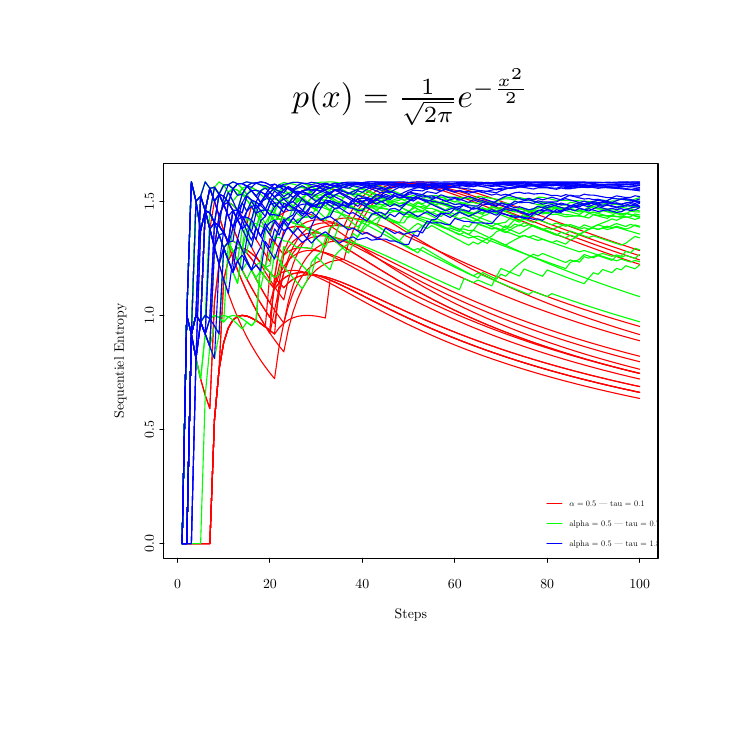
\begin{tikzpicture}[x=1pt,y=1pt]
\definecolor{fillColor}{RGB}{255,255,255}
\path[use as bounding box,fill=fillColor,fill opacity=0.00] (0,0) rectangle (252.94,252.94);
\begin{scope}
\path[clip] ( 49.20, 61.20) rectangle (227.75,203.75);
\definecolor{drawColor}{RGB}{255,0,0}

\path[draw=drawColor,line width= 0.4pt,line join=round,line cap=round] ( 55.81, 66.48) --
	( 57.48, 66.48) --
	( 59.15,142.23) --
	( 60.82,148.97) --
	( 62.49,146.57) --
	( 64.16,186.85) --
	( 65.83,194.89) --
	( 67.50,195.27) --
	( 69.17,192.73) --
	( 70.84,189.02) --
	( 72.51,184.89) --
	( 74.18,180.68) --
	( 75.85,176.58) --
	( 77.52,172.65) --
	( 79.19,168.93) --
	( 80.86,165.42) --
	( 82.53,162.13) --
	( 84.20,159.04) --
	( 85.87,156.15) --
	( 87.54,153.43) --
	( 89.21,150.87) --
	( 90.88,158.71) --
	( 92.55,164.35) --
	( 94.22,168.48) --
	( 95.89,171.51) --
	( 97.56,173.73) --
	( 99.23,175.33) --
	(100.90,176.43) --
	(102.57,177.15) --
	(104.24,177.56) --
	(105.91,177.72) --
	(107.58,177.69) --
	(109.25,177.49) --
	(110.92,177.15) --
	(112.59,176.71) --
	(114.26,176.18) --
	(115.93,175.58) --
	(117.60,174.92) --
	(119.27,174.22) --
	(120.94,173.48) --
	(122.61,172.71) --
	(124.28,171.91) --
	(125.95,171.10) --
	(127.62,170.28) --
	(129.29,169.44) --
	(130.96,168.60) --
	(132.63,167.76) --
	(134.30,166.92) --
	(135.97,166.07) --
	(137.64,165.23) --
	(139.31,164.40) --
	(140.98,163.57) --
	(142.65,162.75) --
	(144.32,161.93) --
	(145.99,161.12) --
	(147.66,160.32) --
	(149.33,159.53) --
	(151.00,158.75) --
	(152.67,157.98) --
	(154.34,157.22) --
	(156.01,156.47) --
	(157.68,155.72) --
	(159.35,154.99) --
	(161.02,154.27) --
	(162.69,153.56) --
	(164.36,152.86) --
	(166.03,152.17) --
	(167.70,151.48) --
	(169.37,150.81) --
	(171.04,150.15) --
	(172.71,149.50) --
	(174.38,148.86) --
	(176.05,148.22) --
	(177.71,147.60) --
	(179.38,146.99) --
	(181.05,146.38) --
	(182.72,145.78) --
	(184.39,145.20) --
	(186.06,144.62) --
	(187.73,144.05) --
	(189.40,143.48) --
	(191.07,142.93) --
	(192.74,142.38) --
	(194.41,141.85) --
	(196.08,141.32) --
	(197.75,140.79) --
	(199.42,140.28) --
	(201.09,139.77) --
	(202.76,139.27) --
	(204.43,138.78) --
	(206.10,138.29) --
	(207.77,137.81) --
	(209.44,137.34) --
	(211.11,136.87) --
	(212.78,136.41) --
	(214.45,135.96) --
	(216.12,135.51) --
	(217.79,135.07) --
	(219.46,134.64) --
	(221.13,134.21);
\end{scope}
\begin{scope}
\path[clip] (  0.00,  0.00) rectangle (252.94,252.94);
\definecolor{drawColor}{RGB}{0,0,0}

\path[draw=drawColor,line width= 0.4pt,line join=round,line cap=round] ( 54.14, 61.20) -- (221.13, 61.20);

\path[draw=drawColor,line width= 0.4pt,line join=round,line cap=round] ( 54.14, 61.20) -- ( 54.14, 59.77);

\path[draw=drawColor,line width= 0.4pt,line join=round,line cap=round] ( 87.54, 61.20) -- ( 87.54, 59.77);

\path[draw=drawColor,line width= 0.4pt,line join=round,line cap=round] (120.94, 61.20) -- (120.94, 59.77);

\path[draw=drawColor,line width= 0.4pt,line join=round,line cap=round] (154.34, 61.20) -- (154.34, 59.77);

\path[draw=drawColor,line width= 0.4pt,line join=round,line cap=round] (187.73, 61.20) -- (187.73, 59.77);

\path[draw=drawColor,line width= 0.4pt,line join=round,line cap=round] (221.13, 61.20) -- (221.13, 59.77);

\node[text=drawColor,anchor=base,inner sep=0pt, outer sep=0pt, scale=  0.50] at ( 54.14, 50.40) {0};

\node[text=drawColor,anchor=base,inner sep=0pt, outer sep=0pt, scale=  0.50] at ( 87.54, 50.40) {20};

\node[text=drawColor,anchor=base,inner sep=0pt, outer sep=0pt, scale=  0.50] at (120.94, 50.40) {40};

\node[text=drawColor,anchor=base,inner sep=0pt, outer sep=0pt, scale=  0.50] at (154.34, 50.40) {60};

\node[text=drawColor,anchor=base,inner sep=0pt, outer sep=0pt, scale=  0.50] at (187.73, 50.40) {80};

\node[text=drawColor,anchor=base,inner sep=0pt, outer sep=0pt, scale=  0.50] at (221.13, 50.40) {100};

\path[draw=drawColor,line width= 0.4pt,line join=round,line cap=round] ( 49.20, 66.48) -- ( 49.20,190.22);

\path[draw=drawColor,line width= 0.4pt,line join=round,line cap=round] ( 49.20, 66.48) -- ( 47.77, 66.48);

\path[draw=drawColor,line width= 0.4pt,line join=round,line cap=round] ( 49.20,107.73) -- ( 47.77,107.73);

\path[draw=drawColor,line width= 0.4pt,line join=round,line cap=round] ( 49.20,148.97) -- ( 47.77,148.97);

\path[draw=drawColor,line width= 0.4pt,line join=round,line cap=round] ( 49.20,190.22) -- ( 47.77,190.22);

\node[text=drawColor,rotate= 90.00,anchor=base,inner sep=0pt, outer sep=0pt, scale=  0.50] at ( 45.60, 66.48) {0.0};

\node[text=drawColor,rotate= 90.00,anchor=base,inner sep=0pt, outer sep=0pt, scale=  0.50] at ( 45.60,107.73) {0.5};

\node[text=drawColor,rotate= 90.00,anchor=base,inner sep=0pt, outer sep=0pt, scale=  0.50] at ( 45.60,148.97) {1.0};

\node[text=drawColor,rotate= 90.00,anchor=base,inner sep=0pt, outer sep=0pt, scale=  0.50] at ( 45.60,190.22) {1.5};

\path[draw=drawColor,line width= 0.4pt,line join=round,line cap=round] ( 49.20, 61.20) --
	(227.75, 61.20) --
	(227.75,203.75) --
	( 49.20,203.75) --
	( 49.20, 61.20);
\end{scope}
\begin{scope}
\path[clip] (  0.00,  0.00) rectangle (252.94,252.94);
\definecolor{drawColor}{RGB}{0,0,0}

\node[text=drawColor,anchor=base,inner sep=0pt, outer sep=0pt, scale=  0.50] at (138.47, 39.60) {Steps};

\node[text=drawColor,rotate= 90.00,anchor=base,inner sep=0pt, outer sep=0pt, scale=  0.50] at ( 34.80,132.47) {Sequentiel Entropy};
\end{scope}
\begin{scope}
\path[clip] ( 49.20, 61.20) rectangle (227.75,203.75);
\definecolor{drawColor}{RGB}{255,0,0}

\path[draw=drawColor,line width= 0.4pt,line join=round,line cap=round] ( 55.81, 66.48) --
	( 57.48, 66.48) --
	( 59.15,142.23) --
	( 60.82,148.97) --
	( 62.49,146.57) --
	( 64.16,142.23) --
	( 65.83,137.68) --
	( 67.50,173.62) --
	( 69.17,184.90) --
	( 70.84,189.02) --
	( 72.51,189.80) --
	( 74.18,188.84) --
	( 75.85,186.96) --
	( 77.52,184.57) --
	( 79.19,181.93) --
	( 80.86,188.34) --
	( 82.53,185.82) --
	( 84.20,183.23) --
	( 85.87,180.63) --
	( 87.54,178.07) --
	( 89.21,182.79) --
	( 90.88,184.89) --
	( 92.55,186.17) --
	( 94.22,186.85) --
	( 95.89,187.07) --
	( 97.56,186.96) --
	( 99.23,186.58) --
	(100.90,185.99) --
	(102.57,185.26) --
	(104.24,184.40) --
	(105.91,183.45) --
	(107.58,182.43) --
	(109.25,181.36) --
	(110.92,180.26) --
	(112.59,179.13) --
	(114.26,177.98) --
	(115.93,176.82) --
	(117.60,175.66) --
	(119.27,174.50) --
	(120.94,173.34) --
	(122.61,172.20) --
	(124.28,171.06) --
	(125.95,169.93) --
	(127.62,168.82) --
	(129.29,167.73) --
	(130.96,166.65) --
	(132.63,165.58) --
	(134.30,164.54) --
	(135.97,163.51) --
	(137.64,162.50) --
	(139.31,161.50) --
	(140.98,160.53) --
	(142.65,159.57) --
	(144.32,158.63) --
	(145.99,157.71) --
	(147.66,156.80) --
	(149.33,155.91) --
	(151.00,155.04) --
	(152.67,154.18) --
	(154.34,153.34) --
	(156.01,152.52) --
	(157.68,151.71) --
	(159.35,150.91) --
	(161.02,150.13) --
	(162.69,149.37) --
	(164.36,148.62) --
	(166.03,147.88) --
	(167.70,147.16) --
	(169.37,146.45) --
	(171.04,145.75) --
	(172.71,145.06) --
	(174.38,144.39) --
	(176.05,143.73) --
	(177.71,143.08) --
	(179.38,142.44) --
	(181.05,141.82) --
	(182.72,141.20) --
	(184.39,140.60) --
	(186.06,140.00) --
	(187.73,139.42) --
	(189.40,138.84) --
	(191.07,138.28) --
	(192.74,137.72) --
	(194.41,137.17) --
	(196.08,136.64) --
	(197.75,136.11) --
	(199.42,135.59) --
	(201.09,135.07) --
	(202.76,134.57) --
	(204.43,134.07) --
	(206.10,133.59) --
	(207.77,133.11) --
	(209.44,132.63) --
	(211.11,132.17) --
	(212.78,131.71) --
	(214.45,131.25) --
	(216.12,130.81) --
	(217.79,130.37) --
	(219.46,129.94) --
	(221.13,129.51);

\path[draw=drawColor,line width= 0.4pt,line join=round,line cap=round] ( 55.81, 66.48) --
	( 57.48,148.97) --
	( 59.15,142.23) --
	( 60.82,133.40) --
	( 62.49,126.03) --
	( 64.16,120.10) --
	( 65.83,115.29) --
	( 67.50,154.03) --
	( 69.17,167.48) --
	( 70.84,173.34) --
	( 72.51,175.55) --
	( 74.18,175.78) --
	( 75.85,174.90) --
	( 77.52,173.37) --
	( 79.19,171.48) --
	( 80.86,169.39) --
	( 82.53,167.21) --
	( 84.20,164.99) --
	( 85.87,162.78) --
	( 87.54,160.61) --
	( 89.21,158.50) --
	( 90.88,160.79) --
	( 92.55,162.38) --
	( 94.22,163.43) --
	( 95.89,164.06) --
	( 97.56,164.37) --
	( 99.23,164.43) --
	(100.90,164.28) --
	(102.57,163.98) --
	(104.24,163.55) --
	(105.91,163.01) --
	(107.58,162.40) --
	(109.25,161.73) --
	(110.92,161.01) --
	(112.59,160.24) --
	(114.26,159.46) --
	(115.93,158.65) --
	(117.60,157.82) --
	(119.27,156.98) --
	(120.94,156.14) --
	(122.61,155.30) --
	(124.28,154.46) --
	(125.95,153.61) --
	(127.62,152.78) --
	(129.29,151.95) --
	(130.96,151.12) --
	(132.63,150.31) --
	(134.30,149.50) --
	(135.97,148.71) --
	(137.64,147.92) --
	(139.31,147.15) --
	(140.98,146.39) --
	(142.65,145.63) --
	(144.32,144.89) --
	(145.99,144.16) --
	(147.66,143.45) --
	(149.33,142.74) --
	(151.00,142.05) --
	(152.67,141.36) --
	(154.34,140.69) --
	(156.01,140.03) --
	(157.68,139.38) --
	(159.35,138.74) --
	(161.02,138.11) --
	(162.69,137.50) --
	(164.36,136.89) --
	(166.03,136.29) --
	(167.70,135.71) --
	(169.37,135.13) --
	(171.04,134.56) --
	(172.71,134.00) --
	(174.38,133.45) --
	(176.05,132.91) --
	(177.71,132.38) --
	(179.38,131.86) --
	(181.05,131.35) --
	(182.72,130.84) --
	(184.39,130.35) --
	(186.06,129.86) --
	(187.73,129.38) --
	(189.40,128.90) --
	(191.07,128.44) --
	(192.74,127.98) --
	(194.41,127.53) --
	(196.08,127.08) --
	(197.75,126.64) --
	(199.42,126.21) --
	(201.09,125.79) --
	(202.76,125.37) --
	(204.43,124.96) --
	(206.10,124.55) --
	(207.77,124.15) --
	(209.44,123.76) --
	(211.11,123.37) --
	(212.78,122.99) --
	(214.45,122.61) --
	(216.12,122.24) --
	(217.79,121.88) --
	(219.46,121.51) --
	(221.13,121.16);

\path[draw=drawColor,line width= 0.4pt,line join=round,line cap=round] ( 55.81, 66.48) --
	( 57.48, 66.48) --
	( 59.15,142.23) --
	( 60.82,148.97) --
	( 62.49,146.57) --
	( 64.16,186.85) --
	( 65.83,194.89) --
	( 67.50,190.22) --
	( 69.17,184.90) --
	( 70.84,179.57) --
	( 72.51,174.49) --
	( 74.18,169.73) --
	( 75.85,165.32) --
	( 77.52,161.25) --
	( 79.19,157.49) --
	( 80.86,154.03) --
	( 82.53,150.82) --
	( 84.20,147.85) --
	( 85.87,145.09) --
	( 87.54,142.53) --
	( 89.21,140.14) --
	( 90.88,137.91) --
	( 92.55,135.81) --
	( 94.22,144.07) --
	( 95.89,150.24) --
	( 97.56,154.97) --
	( 99.23,158.63) --
	(100.90,161.47) --
	(102.57,163.68) --
	(104.24,165.38) --
	(105.91,166.67) --
	(107.58,167.62) --
	(109.25,168.31) --
	(110.92,168.76) --
	(112.59,169.03) --
	(114.26,169.14) --
	(115.93,175.01) --
	(117.60,179.60) --
	(119.27,183.25) --
	(120.94,186.20) --
	(122.61,188.60) --
	(124.28,190.54) --
	(125.95,192.11) --
	(127.62,193.37) --
	(129.29,194.37) --
	(130.96,195.15) --
	(132.63,195.74) --
	(134.30,196.16) --
	(135.97,196.45) --
	(137.64,196.62) --
	(139.31,196.67) --
	(140.98,196.64) --
	(142.65,196.53) --
	(144.32,196.34) --
	(145.99,196.10) --
	(147.66,195.80) --
	(149.33,195.45) --
	(151.00,195.07) --
	(152.67,194.64) --
	(154.34,194.19) --
	(156.01,193.70) --
	(157.68,193.20) --
	(159.35,192.67) --
	(161.02,192.12) --
	(162.69,191.56) --
	(164.36,190.99) --
	(166.03,190.40) --
	(167.70,189.80) --
	(169.37,189.20) --
	(171.04,188.59) --
	(172.71,187.97) --
	(174.38,187.35) --
	(176.05,186.73) --
	(177.71,186.10) --
	(179.38,185.47) --
	(181.05,184.84) --
	(182.72,184.22) --
	(184.39,183.59) --
	(186.06,182.96) --
	(187.73,182.33) --
	(189.40,181.71) --
	(191.07,181.09) --
	(192.74,180.47) --
	(194.41,179.85) --
	(196.08,179.24) --
	(197.75,178.63) --
	(199.42,178.03) --
	(201.09,177.42) --
	(202.76,176.82) --
	(204.43,176.23) --
	(206.10,175.64) --
	(207.77,175.05) --
	(209.44,174.47) --
	(211.11,173.90) --
	(212.78,173.33) --
	(214.45,172.76) --
	(216.12,172.19) --
	(217.79,171.64) --
	(219.46,171.08) --
	(221.13,170.54);

\path[draw=drawColor,line width= 0.4pt,line join=round,line cap=round] ( 55.81, 66.48) --
	( 57.48, 66.48) --
	( 59.15, 66.48) --
	( 60.82, 66.48) --
	( 62.49, 66.48) --
	( 64.16, 66.48) --
	( 65.83, 66.48) --
	( 67.50,111.32) --
	( 69.17,129.52) --
	( 70.84,139.18) --
	( 72.51,144.49) --
	( 74.18,147.31) --
	( 75.85,148.62) --
	( 77.52,148.97) --
	( 79.19,148.71) --
	( 80.86,148.04) --
	( 82.53,147.11) --
	( 84.20,146.01) --
	( 85.87,144.80) --
	( 87.54,164.51) --
	( 89.21,162.65) --
	( 90.88,163.98) --
	( 92.55,164.78) --
	( 94.22,165.17) --
	( 95.89,165.26) --
	( 97.56,165.11) --
	( 99.23,164.77) --
	(100.90,164.28) --
	(102.57,163.68) --
	(104.24,163.00) --
	(105.91,162.24) --
	(107.58,161.44) --
	(109.25,160.59) --
	(110.92,159.72) --
	(112.59,158.82) --
	(114.26,157.92) --
	(115.93,157.00) --
	(117.60,156.08) --
	(119.27,155.17) --
	(120.94,154.25) --
	(122.61,153.34) --
	(124.28,152.44) --
	(125.95,151.55) --
	(127.62,150.66) --
	(129.29,149.79) --
	(130.96,148.93) --
	(132.63,148.08) --
	(134.30,147.25) --
	(135.97,146.43) --
	(137.64,145.62) --
	(139.31,144.83) --
	(140.98,144.05) --
	(142.65,143.28) --
	(144.32,142.53) --
	(145.99,141.79) --
	(147.66,141.06) --
	(149.33,140.34) --
	(151.00,139.64) --
	(152.67,138.96) --
	(154.34,138.28) --
	(156.01,137.62) --
	(157.68,136.96) --
	(159.35,136.32) --
	(161.02,135.70) --
	(162.69,135.08) --
	(164.36,134.47) --
	(166.03,133.88) --
	(167.70,133.29) --
	(169.37,132.72) --
	(171.04,132.16) --
	(172.71,131.60) --
	(174.38,131.06) --
	(176.05,130.52) --
	(177.71,130.00) --
	(179.38,129.48) --
	(181.05,128.97) --
	(182.72,128.47) --
	(184.39,127.98) --
	(186.06,127.50) --
	(187.73,127.03) --
	(189.40,126.56) --
	(191.07,126.10) --
	(192.74,125.65) --
	(194.41,125.20) --
	(196.08,124.77) --
	(197.75,124.34) --
	(199.42,123.91) --
	(201.09,123.50) --
	(202.76,123.09) --
	(204.43,122.68) --
	(206.10,122.28) --
	(207.77,121.89) --
	(209.44,121.51) --
	(211.11,121.13) --
	(212.78,120.75) --
	(214.45,120.38) --
	(216.12,120.02) --
	(217.79,119.66) --
	(219.46,119.31) --
	(221.13,118.96);

\path[draw=drawColor,line width= 0.4pt,line join=round,line cap=round] ( 55.81, 66.48) --
	( 57.48, 66.48) --
	( 59.15, 66.48) --
	( 60.82, 66.48) --
	( 62.49, 66.48) --
	( 64.16, 66.48) --
	( 65.83, 66.48) --
	( 67.50,111.32) --
	( 69.17,129.52) --
	( 70.84,139.18) --
	( 72.51,144.49) --
	( 74.18,147.31) --
	( 75.85,148.62) --
	( 77.52,148.97) --
	( 79.19,148.71) --
	( 80.86,148.04) --
	( 82.53,147.11) --
	( 84.20,146.01) --
	( 85.87,144.80) --
	( 87.54,143.53) --
	( 89.21,162.65) --
	( 90.88,160.79) --
	( 92.55,158.97) --
	( 94.22,160.78) --
	( 95.89,162.05) --
	( 97.56,162.90) --
	( 99.23,163.41) --
	(100.90,163.65) --
	(102.57,163.68) --
	(104.24,163.55) --
	(105.91,163.27) --
	(107.58,162.88) --
	(109.25,162.41) --
	(110.92,161.86) --
	(112.59,161.25) --
	(114.26,160.60) --
	(115.93,159.91) --
	(117.60,159.20) --
	(119.27,158.46) --
	(120.94,157.70) --
	(122.61,156.94) --
	(124.28,156.16) --
	(125.95,155.39) --
	(127.62,154.61) --
	(129.29,153.83) --
	(130.96,153.05) --
	(132.63,152.27) --
	(134.30,151.51) --
	(135.97,150.74) --
	(137.64,149.99) --
	(139.31,149.24) --
	(140.98,148.50) --
	(142.65,147.77) --
	(144.32,147.04) --
	(145.99,146.33) --
	(147.66,145.63) --
	(149.33,144.94) --
	(151.00,144.25) --
	(152.67,143.58) --
	(154.34,142.91) --
	(156.01,142.26) --
	(157.68,141.62) --
	(159.35,140.98) --
	(161.02,140.36) --
	(162.69,139.74) --
	(164.36,139.14) --
	(166.03,138.54) --
	(167.70,137.96) --
	(169.37,137.38) --
	(171.04,136.81) --
	(172.71,136.25) --
	(174.38,135.70) --
	(176.05,135.16) --
	(177.71,134.63) --
	(179.38,134.10) --
	(181.05,133.59) --
	(182.72,133.08) --
	(184.39,132.58) --
	(186.06,132.08) --
	(187.73,131.60) --
	(189.40,131.12) --
	(191.07,130.65) --
	(192.74,130.18) --
	(194.41,129.73) --
	(196.08,129.28) --
	(197.75,128.83) --
	(199.42,128.40) --
	(201.09,127.97) --
	(202.76,127.54) --
	(204.43,127.12) --
	(206.10,126.71) --
	(207.77,126.31) --
	(209.44,125.90) --
	(211.11,125.51) --
	(212.78,125.12) --
	(214.45,124.74) --
	(216.12,124.36) --
	(217.79,123.99) --
	(219.46,123.62) --
	(221.13,123.26);

\path[draw=drawColor,line width= 0.4pt,line join=round,line cap=round] ( 55.81, 66.48) --
	( 57.48, 66.48) --
	( 59.15,142.23) --
	( 60.82,190.22) --
	( 62.49,192.03) --
	( 64.16,186.85) --
	( 65.83,180.22) --
	( 67.50,182.43) --
	( 69.17,181.32) --
	( 70.84,178.75) --
	( 72.51,175.55) --
	( 74.18,172.12) --
	( 75.85,168.68) --
	( 77.52,165.31) --
	( 79.19,162.08) --
	( 80.86,159.01) --
	( 82.53,156.09) --
	( 84.20,153.34) --
	( 85.87,150.74) --
	( 87.54,148.29) --
	( 89.21,145.98) --
	( 90.88,156.87) --
	( 92.55,164.35) --
	( 94.22,169.73) --
	( 95.89,173.67) --
	( 97.56,176.58) --
	( 99.23,178.70) --
	(100.90,180.22) --
	(102.57,181.26) --
	(104.24,181.93) --
	(105.91,182.30) --
	(107.58,182.43) --
	(109.25,182.37) --
	(110.92,182.14) --
	(112.59,181.78) --
	(114.26,181.32) --
	(115.93,180.77) --
	(117.60,180.33) --
	(119.27,179.82) --
	(120.94,183.46) --
	(122.61,186.40) --
	(124.28,188.80) --
	(125.95,190.76) --
	(127.62,192.35) --
	(129.29,193.64) --
	(130.96,194.67) --
	(132.63,195.48) --
	(134.30,196.11) --
	(135.97,196.57) --
	(137.64,196.89) --
	(139.31,197.09) --
	(140.98,197.18) --
	(142.65,197.18) --
	(144.32,197.10) --
	(145.99,196.95) --
	(147.66,196.74) --
	(149.33,196.47) --
	(151.00,196.16) --
	(152.67,195.80) --
	(154.34,195.40) --
	(156.01,194.97) --
	(157.68,194.52) --
	(159.35,194.04) --
	(161.02,193.53) --
	(162.69,193.01) --
	(164.36,192.47) --
	(166.03,191.92) --
	(167.70,191.35) --
	(169.37,190.78) --
	(171.04,190.19) --
	(172.71,189.60) --
	(174.38,189.00) --
	(176.05,188.40) --
	(177.71,187.79) --
	(179.38,187.18) --
	(181.05,186.57) --
	(182.72,185.95) --
	(184.39,185.34) --
	(186.06,184.72) --
	(187.73,184.11) --
	(189.40,183.49) --
	(191.07,182.88) --
	(192.74,182.27) --
	(194.41,181.66) --
	(196.08,181.05) --
	(197.75,180.45) --
	(199.42,179.85) --
	(201.09,179.25) --
	(202.76,178.66) --
	(204.43,178.07) --
	(206.10,177.48) --
	(207.77,176.90) --
	(209.44,176.32) --
	(211.11,175.75) --
	(212.78,175.17) --
	(214.45,174.61) --
	(216.12,174.05) --
	(217.79,173.49) --
	(219.46,172.94) --
	(221.13,172.39);

\path[draw=drawColor,line width= 0.4pt,line join=round,line cap=round] ( 55.81, 66.48) --
	( 57.48, 66.48) --
	( 59.15, 66.48) --
	( 60.82, 66.48) --
	( 62.49, 66.48) --
	( 64.16, 66.48) --
	( 65.83, 66.48) --
	( 67.50,111.32) --
	( 69.17,129.52) --
	( 70.84,139.18) --
	( 72.51,144.49) --
	( 74.18,147.31) --
	( 75.85,148.62) --
	( 77.52,148.97) --
	( 79.19,148.71) --
	( 80.86,148.04) --
	( 82.53,147.11) --
	( 84.20,168.16) --
	( 85.87,166.36) --
	( 87.54,176.74) --
	( 89.21,174.77) --
	( 90.88,181.52) --
	( 92.55,186.17) --
	( 94.22,189.39) --
	( 95.89,191.59) --
	( 97.56,193.04) --
	( 99.23,193.92) --
	(100.90,194.89) --
	(102.57,195.43) --
	(104.24,195.63) --
	(105.91,195.56) --
	(107.58,195.27) --
	(109.25,194.82) --
	(110.92,194.22) --
	(112.59,193.52) --
	(114.26,192.73) --
	(115.93,191.87) --
	(117.60,190.96) --
	(119.27,190.01) --
	(120.94,189.02) --
	(122.61,188.01) --
	(124.28,186.98) --
	(125.95,185.93) --
	(127.62,184.89) --
	(129.29,183.83) --
	(130.96,182.78) --
	(132.63,181.73) --
	(134.30,180.68) --
	(135.97,179.64) --
	(137.64,178.61) --
	(139.31,177.59) --
	(140.98,176.58) --
	(142.65,175.58) --
	(144.32,174.59) --
	(145.99,173.61) --
	(147.66,172.65) --
	(149.33,171.70) --
	(151.00,170.76) --
	(152.67,169.84) --
	(154.34,168.93) --
	(156.01,168.03) --
	(157.68,167.15) --
	(159.35,166.28) --
	(161.02,165.42) --
	(162.69,164.58) --
	(164.36,163.75) --
	(166.03,162.94) --
	(167.70,162.13) --
	(169.37,161.34) --
	(171.04,160.56) --
	(172.71,159.80) --
	(174.38,159.04) --
	(176.05,158.30) --
	(177.71,157.57) --
	(179.38,156.85) --
	(181.05,156.15) --
	(182.72,155.45) --
	(184.39,154.77) --
	(186.06,154.09) --
	(187.73,153.43) --
	(189.40,152.77) --
	(191.07,152.13) --
	(192.74,151.50) --
	(194.41,150.87) --
	(196.08,150.26) --
	(197.75,149.65) --
	(199.42,149.05) --
	(201.09,148.47) --
	(202.76,147.89) --
	(204.43,147.32) --
	(206.10,146.76) --
	(207.77,146.20) --
	(209.44,145.66) --
	(211.11,145.12) --
	(212.78,144.59) --
	(214.45,144.07) --
	(216.12,143.55) --
	(217.79,143.05) --
	(219.46,142.54) --
	(221.13,142.05);

\path[draw=drawColor,line width= 0.4pt,line join=round,line cap=round] ( 55.81, 66.48) --
	( 57.48, 66.48) --
	( 59.15,142.23) --
	( 60.82,190.22) --
	( 62.49,192.03) --
	( 64.16,186.85) --
	( 65.83,180.22) --
	( 67.50,182.43) --
	( 69.17,181.32) --
	( 70.84,178.75) --
	( 72.51,175.55) --
	( 74.18,172.12) --
	( 75.85,168.68) --
	( 77.52,165.31) --
	( 79.19,162.08) --
	( 80.86,159.01) --
	( 82.53,156.09) --
	( 84.20,153.34) --
	( 85.87,150.74) --
	( 87.54,148.29) --
	( 89.21,159.32) --
	( 90.88,163.57) --
	( 92.55,166.65) --
	( 94.22,168.85) --
	( 95.89,170.40) --
	( 97.56,171.43) --
	( 99.23,172.07) --
	(100.90,172.39) --
	(102.57,172.46) --
	(104.24,172.34) --
	(105.91,172.05) --
	(107.58,171.64) --
	(109.25,171.12) --
	(110.92,170.52) --
	(112.59,169.86) --
	(114.26,169.14) --
	(115.93,168.38) --
	(117.60,167.59) --
	(119.27,166.78) --
	(120.94,165.95) --
	(122.61,165.10) --
	(124.28,164.25) --
	(125.95,163.39) --
	(127.62,162.52) --
	(129.29,161.66) --
	(130.96,160.80) --
	(132.63,159.95) --
	(134.30,159.10) --
	(135.97,158.26) --
	(137.64,157.43) --
	(139.31,156.60) --
	(140.98,155.78) --
	(142.65,154.98) --
	(144.32,154.18) --
	(145.99,153.40) --
	(147.66,152.62) --
	(149.33,151.86) --
	(151.00,151.10) --
	(152.67,150.36) --
	(154.34,149.63) --
	(156.01,148.91) --
	(157.68,148.20) --
	(159.35,147.51) --
	(161.02,146.82) --
	(162.69,146.14) --
	(164.36,145.48) --
	(166.03,144.82) --
	(167.70,144.18) --
	(169.37,143.55) --
	(171.04,142.92) --
	(172.71,142.31) --
	(174.38,141.70) --
	(176.05,141.11) --
	(177.71,140.52) --
	(179.38,139.95) --
	(181.05,139.38) --
	(182.72,138.82) --
	(184.39,138.27) --
	(186.06,137.73) --
	(187.73,137.20) --
	(189.40,136.67) --
	(191.07,136.16) --
	(192.74,135.65) --
	(194.41,135.15) --
	(196.08,134.65) --
	(197.75,134.17) --
	(199.42,133.69) --
	(201.09,133.22) --
	(202.76,132.75) --
	(204.43,132.29) --
	(206.10,131.84) --
	(207.77,131.40) --
	(209.44,130.96) --
	(211.11,130.53) --
	(212.78,130.10) --
	(214.45,129.68) --
	(216.12,129.27) --
	(217.79,128.86) --
	(219.46,128.46) --
	(221.13,128.06);

\path[draw=drawColor,line width= 0.4pt,line join=round,line cap=round] ( 55.81, 66.48) --
	( 57.48, 66.48) --
	( 59.15, 66.48) --
	( 60.82, 66.48) --
	( 62.49, 66.48) --
	( 64.16, 66.48) --
	( 65.83, 66.48) --
	( 67.50,111.32) --
	( 69.17,129.52) --
	( 70.84,139.18) --
	( 72.51,144.49) --
	( 74.18,147.31) --
	( 75.85,148.62) --
	( 77.52,148.97) --
	( 79.19,148.71) --
	( 80.86,148.04) --
	( 82.53,147.11) --
	( 84.20,146.01) --
	( 85.87,144.80) --
	( 87.54,143.53) --
	( 89.21,162.65) --
	( 90.88,160.79) --
	( 92.55,158.97) --
	( 94.22,160.78) --
	( 95.89,162.05) --
	( 97.56,162.90) --
	( 99.23,163.41) --
	(100.90,163.65) --
	(102.57,163.68) --
	(104.24,163.55) --
	(105.91,163.27) --
	(107.58,162.88) --
	(109.25,162.41) --
	(110.92,161.86) --
	(112.59,161.25) --
	(114.26,160.60) --
	(115.93,159.91) --
	(117.60,159.20) --
	(119.27,158.46) --
	(120.94,157.70) --
	(122.61,156.94) --
	(124.28,156.16) --
	(125.95,155.39) --
	(127.62,154.61) --
	(129.29,153.83) --
	(130.96,153.05) --
	(132.63,152.27) --
	(134.30,151.51) --
	(135.97,150.74) --
	(137.64,149.99) --
	(139.31,149.24) --
	(140.98,148.50) --
	(142.65,147.77) --
	(144.32,147.04) --
	(145.99,146.33) --
	(147.66,145.63) --
	(149.33,144.94) --
	(151.00,144.25) --
	(152.67,143.58) --
	(154.34,142.91) --
	(156.01,142.26) --
	(157.68,141.62) --
	(159.35,140.98) --
	(161.02,140.36) --
	(162.69,139.74) --
	(164.36,139.14) --
	(166.03,138.54) --
	(167.70,137.96) --
	(169.37,137.38) --
	(171.04,136.81) --
	(172.71,136.25) --
	(174.38,135.70) --
	(176.05,135.16) --
	(177.71,134.63) --
	(179.38,134.10) --
	(181.05,133.59) --
	(182.72,133.08) --
	(184.39,132.58) --
	(186.06,132.08) --
	(187.73,131.60) --
	(189.40,131.12) --
	(191.07,130.65) --
	(192.74,130.18) --
	(194.41,129.73) --
	(196.08,129.28) --
	(197.75,128.83) --
	(199.42,128.40) --
	(201.09,127.97) --
	(202.76,127.54) --
	(204.43,127.12) --
	(206.10,126.71) --
	(207.77,126.31) --
	(209.44,125.90) --
	(211.11,125.51) --
	(212.78,125.12) --
	(214.45,124.74) --
	(216.12,124.36) --
	(217.79,123.99) --
	(219.46,123.62) --
	(221.13,123.26);

\path[draw=drawColor,line width= 0.4pt,line join=round,line cap=round] ( 55.81, 66.48) --
	( 57.48, 66.48) --
	( 59.15,142.23) --
	( 60.82,148.97) --
	( 62.49,192.03) --
	( 64.16,186.85) --
	( 65.83,180.22) --
	( 67.50,173.62) --
	( 69.17,167.48) --
	( 70.84,161.90) --
	( 72.51,156.87) --
	( 74.18,152.34) --
	( 75.85,148.25) --
	( 77.52,144.55) --
	( 79.19,141.18) --
	( 80.86,138.11) --
	( 82.53,135.31) --
	( 84.20,132.73) --
	( 85.87,130.35) --
	( 87.54,128.15) --
	( 89.21,126.11) --
	( 90.88,137.91) --
	( 92.55,146.20) --
	( 94.22,152.34) --
	( 95.89,156.98) --
	( 97.56,160.53) --
	( 99.23,163.24) --
	(100.90,165.31) --
	(102.57,166.87) --
	(104.24,168.02) --
	(105.91,168.84) --
	(107.58,175.09) --
	(109.25,179.85) --
	(110.92,183.55) --
	(112.59,183.94) --
	(114.26,184.13) --
	(115.93,184.15) --
	(117.60,184.03) --
	(119.27,183.79) --
	(120.94,183.46) --
	(122.61,183.04) --
	(124.28,182.55) --
	(125.95,182.01) --
	(127.62,181.42) --
	(129.29,180.79) --
	(130.96,180.13) --
	(132.63,179.44) --
	(134.30,178.73) --
	(135.97,178.00) --
	(137.64,177.25) --
	(139.31,176.50) --
	(140.98,175.74) --
	(142.65,174.97) --
	(144.32,174.20) --
	(145.99,173.43) --
	(147.66,172.66) --
	(149.33,171.88) --
	(151.00,171.11) --
	(152.67,170.35) --
	(154.34,169.59) --
	(156.01,168.83) --
	(157.68,168.08) --
	(159.35,167.33) --
	(161.02,166.59) --
	(162.69,165.86) --
	(164.36,165.13) --
	(166.03,164.42) --
	(167.70,163.70) --
	(169.37,163.00) --
	(171.04,162.31) --
	(172.71,161.62) --
	(174.38,160.94) --
	(176.05,160.27) --
	(177.71,159.60) --
	(179.38,158.95) --
	(181.05,158.30) --
	(182.72,157.66) --
	(184.39,157.03) --
	(186.06,156.40) --
	(187.73,155.79) --
	(189.40,155.18) --
	(191.07,154.58) --
	(192.74,153.99) --
	(194.41,153.40) --
	(196.08,152.82) --
	(197.75,152.25) --
	(199.42,151.69) --
	(201.09,151.13) --
	(202.76,150.59) --
	(204.43,150.04) --
	(206.10,149.51) --
	(207.77,148.98) --
	(209.44,148.46) --
	(211.11,147.94) --
	(212.78,147.44) --
	(214.45,146.94) --
	(216.12,146.44) --
	(217.79,145.95) --
	(219.46,145.47) --
	(221.13,144.99);

\path[draw=drawColor,line width= 0.4pt,line join=round,line cap=round] ( 55.81, 66.48) --
	( 57.48,148.97) --
	( 59.15,142.23) --
	( 60.82,133.40) --
	( 62.49,126.03) --
	( 64.16,120.10) --
	( 65.83,115.29) --
	( 67.50,154.03) --
	( 69.17,167.48) --
	( 70.84,173.34) --
	( 72.51,175.55) --
	( 74.18,175.78) --
	( 75.85,174.90) --
	( 77.52,173.37) --
	( 79.19,171.48) --
	( 80.86,169.39) --
	( 82.53,167.21) --
	( 84.20,164.99) --
	( 85.87,162.78) --
	( 87.54,160.61) --
	( 89.21,158.50) --
	( 90.88,160.79) --
	( 92.55,162.38) --
	( 94.22,163.43) --
	( 95.89,164.06) --
	( 97.56,164.37) --
	( 99.23,164.43) --
	(100.90,164.28) --
	(102.57,163.98) --
	(104.24,163.55) --
	(105.91,163.01) --
	(107.58,162.40) --
	(109.25,161.73) --
	(110.92,161.01) --
	(112.59,160.24) --
	(114.26,159.46) --
	(115.93,158.65) --
	(117.60,157.82) --
	(119.27,156.98) --
	(120.94,156.14) --
	(122.61,155.30) --
	(124.28,154.46) --
	(125.95,153.61) --
	(127.62,152.78) --
	(129.29,151.95) --
	(130.96,151.12) --
	(132.63,150.31) --
	(134.30,149.50) --
	(135.97,148.71) --
	(137.64,147.92) --
	(139.31,147.15) --
	(140.98,146.39) --
	(142.65,145.63) --
	(144.32,144.89) --
	(145.99,144.16) --
	(147.66,143.45) --
	(149.33,142.74) --
	(151.00,142.05) --
	(152.67,141.36) --
	(154.34,140.69) --
	(156.01,140.03) --
	(157.68,139.38) --
	(159.35,138.74) --
	(161.02,138.11) --
	(162.69,137.50) --
	(164.36,136.89) --
	(166.03,136.29) --
	(167.70,135.71) --
	(169.37,135.13) --
	(171.04,134.56) --
	(172.71,134.00) --
	(174.38,133.45) --
	(176.05,132.91) --
	(177.71,132.38) --
	(179.38,131.86) --
	(181.05,131.35) --
	(182.72,130.84) --
	(184.39,130.35) --
	(186.06,129.86) --
	(187.73,129.38) --
	(189.40,128.90) --
	(191.07,128.44) --
	(192.74,127.98) --
	(194.41,127.53) --
	(196.08,127.08) --
	(197.75,126.64) --
	(199.42,126.21) --
	(201.09,125.79) --
	(202.76,125.37) --
	(204.43,124.96) --
	(206.10,124.55) --
	(207.77,124.15) --
	(209.44,123.76) --
	(211.11,123.37) --
	(212.78,122.99) --
	(214.45,122.61) --
	(216.12,122.24) --
	(217.79,121.88) --
	(219.46,121.51) --
	(221.13,121.16);

\path[draw=drawColor,line width= 0.4pt,line join=round,line cap=round] ( 55.81, 66.48) --
	( 57.48, 66.48) --
	( 59.15, 66.48) --
	( 60.82, 66.48) --
	( 62.49, 66.48) --
	( 64.16, 66.48) --
	( 65.83, 66.48) --
	( 67.50,111.32) --
	( 69.17,129.52) --
	( 70.84,139.18) --
	( 72.51,144.49) --
	( 74.18,147.31) --
	( 75.85,148.62) --
	( 77.52,148.97) --
	( 79.19,148.71) --
	( 80.86,148.04) --
	( 82.53,147.11) --
	( 84.20,146.01) --
	( 85.87,144.80) --
	( 87.54,143.53) --
	( 89.21,142.23) --
	( 90.88,160.79) --
	( 92.55,170.80) --
	( 94.22,172.12) --
	( 95.89,172.94) --
	( 97.56,173.37) --
	( 99.23,173.49) --
	(100.90,173.37) --
	(102.57,173.07) --
	(104.24,172.62) --
	(105.91,172.05) --
	(107.58,171.39) --
	(109.25,170.66) --
	(110.92,169.87) --
	(112.59,169.03) --
	(114.26,168.16) --
	(115.93,167.27) --
	(117.60,166.36) --
	(119.27,165.44) --
	(120.94,164.51) --
	(122.61,163.58) --
	(124.28,162.65) --
	(125.95,161.72) --
	(127.62,160.79) --
	(129.29,159.88) --
	(130.96,158.97) --
	(132.63,158.07) --
	(134.30,157.18) --
	(135.97,156.30) --
	(137.64,155.43) --
	(139.31,154.58) --
	(140.98,153.73) --
	(142.65,152.90) --
	(144.32,152.09) --
	(145.99,151.28) --
	(147.66,150.49) --
	(149.33,149.71) --
	(151.00,148.95) --
	(152.67,148.19) --
	(154.34,147.45) --
	(156.01,146.72) --
	(157.68,146.01) --
	(159.35,145.30) --
	(161.02,144.61) --
	(162.69,143.93) --
	(164.36,143.26) --
	(166.03,142.61) --
	(167.70,141.96) --
	(169.37,141.33) --
	(171.04,140.70) --
	(172.71,140.09) --
	(174.38,139.48) --
	(176.05,138.89) --
	(177.71,138.31) --
	(179.38,137.73) --
	(181.05,137.17) --
	(182.72,136.61) --
	(184.39,136.07) --
	(186.06,135.53) --
	(187.73,135.00) --
	(189.40,134.48) --
	(191.07,133.97) --
	(192.74,133.46) --
	(194.41,132.97) --
	(196.08,132.48) --
	(197.75,132.00) --
	(199.42,131.53) --
	(201.09,131.06) --
	(202.76,130.60) --
	(204.43,130.15) --
	(206.10,129.70) --
	(207.77,129.26) --
	(209.44,128.83) --
	(211.11,128.41) --
	(212.78,127.99) --
	(214.45,127.57) --
	(216.12,127.17) --
	(217.79,126.76) --
	(219.46,126.37) --
	(221.13,125.98);

\path[draw=drawColor,line width= 0.4pt,line join=round,line cap=round] ( 55.81, 66.48) --
	( 57.48, 66.48) --
	( 59.15,142.23) --
	( 60.82,148.97) --
	( 62.49,146.57) --
	( 64.16,186.85) --
	( 65.83,194.89) --
	( 67.50,195.27) --
	( 69.17,192.73) --
	( 70.84,189.02) --
	( 72.51,184.89) --
	( 74.18,180.68) --
	( 75.85,176.58) --
	( 77.52,172.65) --
	( 79.19,168.93) --
	( 80.86,165.42) --
	( 82.53,162.13) --
	( 84.20,159.04) --
	( 85.87,156.15) --
	( 87.54,153.43) --
	( 89.21,159.32) --
	( 90.88,156.87) --
	( 92.55,154.55) --
	( 94.22,162.02) --
	( 95.89,167.48) --
	( 97.56,171.54) --
	( 99.23,174.59) --
	(100.90,176.86) --
	(102.57,178.54) --
	(104.24,179.74) --
	(105.91,180.57) --
	(107.58,181.09) --
	(109.25,181.36) --
	(110.92,181.44) --
	(112.59,181.34) --
	(114.26,181.11) --
	(115.93,180.77) --
	(117.60,180.33) --
	(119.27,179.82) --
	(120.94,179.24) --
	(122.61,178.62) --
	(124.28,177.94) --
	(125.95,177.24) --
	(127.62,176.50) --
	(129.29,175.75) --
	(130.96,174.97) --
	(132.63,174.19) --
	(134.30,173.39) --
	(135.97,172.59) --
	(137.64,171.78) --
	(139.31,170.97) --
	(140.98,170.16) --
	(142.65,169.35) --
	(144.32,168.54) --
	(145.99,167.74) --
	(147.66,166.94) --
	(149.33,166.15) --
	(151.00,165.36) --
	(152.67,164.59) --
	(154.34,163.81) --
	(156.01,163.05) --
	(157.68,162.29) --
	(159.35,161.55) --
	(161.02,160.81) --
	(162.69,160.08) --
	(164.36,159.36) --
	(166.03,158.64) --
	(167.70,157.94) --
	(169.37,157.25) --
	(171.04,156.56) --
	(172.71,155.89) --
	(174.38,155.22) --
	(176.05,154.56) --
	(177.71,153.91) --
	(179.38,153.27) --
	(181.05,152.64) --
	(182.72,152.02) --
	(184.39,151.40) --
	(186.06,150.80) --
	(187.73,150.20) --
	(189.40,149.61) --
	(191.07,149.03) --
	(192.74,148.46) --
	(194.41,147.89) --
	(196.08,147.33) --
	(197.75,146.78) --
	(199.42,146.24) --
	(201.09,145.70) --
	(202.76,145.18) --
	(204.43,144.66) --
	(206.10,144.14) --
	(207.77,143.63) --
	(209.44,143.13) --
	(211.11,142.64) --
	(212.78,142.15) --
	(214.45,141.67) --
	(216.12,141.20) --
	(217.79,140.73) --
	(219.46,140.27) --
	(221.13,139.81);

\path[draw=drawColor,line width= 0.4pt,line join=round,line cap=round] ( 55.81, 66.48) --
	( 57.48, 66.48) --
	( 59.15, 66.48) --
	( 60.82, 66.48) --
	( 62.49, 66.48) --
	( 64.16, 66.48) --
	( 65.83, 66.48) --
	( 67.50,111.32) --
	( 69.17,129.52) --
	( 70.84,161.90) --
	( 72.51,168.82) --
	( 74.18,172.12) --
	( 75.85,173.37) --
	( 77.52,173.37) --
	( 79.19,172.62) --
	( 80.86,171.39) --
	( 82.53,169.87) --
	( 84.20,168.16) --
	( 85.87,166.36) --
	( 87.54,164.51) --
	( 89.21,162.65) --
	( 90.88,172.78) --
	( 92.55,179.56) --
	( 94.22,180.52) --
	( 95.89,181.00) --
	( 97.56,181.12) --
	( 99.23,180.95) --
	(100.90,180.57) --
	(102.57,180.02) --
	(104.24,179.34) --
	(105.91,178.55) --
	(107.58,177.69) --
	(109.25,176.76) --
	(110.92,175.79) --
	(112.59,174.79) --
	(114.26,173.76) --
	(115.93,172.72) --
	(117.60,171.66) --
	(119.27,170.60) --
	(120.94,169.55) --
	(122.61,168.49) --
	(124.28,167.44) --
	(125.95,166.40) --
	(127.62,165.37) --
	(129.29,164.35) --
	(130.96,163.35) --
	(132.63,162.35) --
	(134.30,161.37) --
	(135.97,160.41) --
	(137.64,159.46) --
	(139.31,158.53) --
	(140.98,157.61) --
	(142.65,156.71) --
	(144.32,155.82) --
	(145.99,154.95) --
	(147.66,154.09) --
	(149.33,153.25) --
	(151.00,152.42) --
	(152.67,151.61) --
	(154.34,150.81) --
	(156.01,150.03) --
	(157.68,149.26) --
	(159.35,148.50) --
	(161.02,147.76) --
	(162.69,147.03) --
	(164.36,146.32) --
	(166.03,145.61) --
	(167.70,144.92) --
	(169.37,144.25) --
	(171.04,143.58) --
	(172.71,142.93) --
	(174.38,142.28) --
	(176.05,141.65) --
	(177.71,141.03) --
	(179.38,140.42) --
	(181.05,139.82) --
	(182.72,139.23) --
	(184.39,138.65) --
	(186.06,138.08) --
	(187.73,137.52) --
	(189.40,136.97) --
	(191.07,136.42) --
	(192.74,135.89) --
	(194.41,135.37) --
	(196.08,134.85) --
	(197.75,134.34) --
	(199.42,133.84) --
	(201.09,133.35) --
	(202.76,132.86) --
	(204.43,132.39) --
	(206.10,131.92) --
	(207.77,131.45) --
	(209.44,131.00) --
	(211.11,130.55) --
	(212.78,130.11) --
	(214.45,129.67) --
	(216.12,129.24) --
	(217.79,128.82) --
	(219.46,128.40) --
	(221.13,127.99);

\path[draw=drawColor,line width= 0.4pt,line join=round,line cap=round] ( 55.81, 66.48) --
	( 57.48, 66.48) --
	( 59.15, 66.48) --
	( 60.82, 66.48) --
	( 62.49, 66.48) --
	( 64.16, 66.48) --
	( 65.83, 66.48) --
	( 67.50,111.32) --
	( 69.17,129.52) --
	( 70.84,161.90) --
	( 72.51,168.82) --
	( 74.18,172.12) --
	( 75.85,173.37) --
	( 77.52,173.37) --
	( 79.19,172.62) --
	( 80.86,171.39) --
	( 82.53,169.87) --
	( 84.20,168.16) --
	( 85.87,166.36) --
	( 87.54,164.51) --
	( 89.21,162.65) --
	( 90.88,172.78) --
	( 92.55,179.56) --
	( 94.22,180.52) --
	( 95.89,181.00) --
	( 97.56,181.12) --
	( 99.23,180.95) --
	(100.90,180.57) --
	(102.57,180.02) --
	(104.24,179.34) --
	(105.91,178.55) --
	(107.58,177.69) --
	(109.25,176.76) --
	(110.92,175.79) --
	(112.59,174.79) --
	(114.26,173.76) --
	(115.93,172.72) --
	(117.60,171.66) --
	(119.27,170.60) --
	(120.94,169.55) --
	(122.61,168.49) --
	(124.28,167.44) --
	(125.95,166.40) --
	(127.62,165.37) --
	(129.29,164.35) --
	(130.96,163.35) --
	(132.63,162.35) --
	(134.30,161.37) --
	(135.97,160.41) --
	(137.64,159.46) --
	(139.31,158.53) --
	(140.98,157.61) --
	(142.65,156.71) --
	(144.32,155.82) --
	(145.99,154.95) --
	(147.66,154.09) --
	(149.33,153.25) --
	(151.00,152.42) --
	(152.67,151.61) --
	(154.34,150.81) --
	(156.01,150.03) --
	(157.68,149.26) --
	(159.35,148.50) --
	(161.02,147.76) --
	(162.69,147.03) --
	(164.36,146.32) --
	(166.03,145.61) --
	(167.70,144.92) --
	(169.37,144.25) --
	(171.04,143.58) --
	(172.71,142.93) --
	(174.38,142.28) --
	(176.05,141.65) --
	(177.71,141.03) --
	(179.38,140.42) --
	(181.05,139.82) --
	(182.72,139.23) --
	(184.39,138.65) --
	(186.06,138.08) --
	(187.73,137.52) --
	(189.40,136.97) --
	(191.07,136.42) --
	(192.74,135.89) --
	(194.41,135.37) --
	(196.08,134.85) --
	(197.75,134.34) --
	(199.42,133.84) --
	(201.09,133.35) --
	(202.76,132.86) --
	(204.43,132.39) --
	(206.10,131.92) --
	(207.77,131.45) --
	(209.44,131.00) --
	(211.11,130.55) --
	(212.78,130.11) --
	(214.45,129.67) --
	(216.12,129.24) --
	(217.79,128.82) --
	(219.46,128.40) --
	(221.13,127.99);

\path[draw=drawColor,line width= 0.4pt,line join=round,line cap=round] ( 55.81, 66.48) --
	( 57.48, 66.48) --
	( 59.15, 66.48) --
	( 60.82, 66.48) --
	( 62.49, 66.48) --
	( 64.16, 66.48) --
	( 65.83, 66.48) --
	( 67.50,111.32) --
	( 69.17,129.52) --
	( 70.84,139.18) --
	( 72.51,144.49) --
	( 74.18,147.31) --
	( 75.85,148.62) --
	( 77.52,148.97) --
	( 79.19,148.71) --
	( 80.86,148.04) --
	( 82.53,147.11) --
	( 84.20,146.01) --
	( 85.87,144.80) --
	( 87.54,143.53) --
	( 89.21,142.23) --
	( 90.88,144.49) --
	( 92.55,146.14) --
	( 94.22,147.31) --
	( 95.89,148.11) --
	( 97.56,148.62) --
	( 99.23,148.89) --
	(100.90,148.97) --
	(102.57,148.90) --
	(104.24,148.71) --
	(105.91,148.41) --
	(107.58,148.04) --
	(109.25,161.73) --
	(110.92,161.01) --
	(112.59,160.24) --
	(114.26,159.46) --
	(115.93,158.65) --
	(117.60,157.82) --
	(119.27,156.98) --
	(120.94,156.14) --
	(122.61,155.30) --
	(124.28,154.46) --
	(125.95,153.61) --
	(127.62,152.78) --
	(129.29,151.95) --
	(130.96,151.12) --
	(132.63,150.31) --
	(134.30,149.50) --
	(135.97,148.71) --
	(137.64,147.92) --
	(139.31,147.15) --
	(140.98,146.39) --
	(142.65,145.63) --
	(144.32,144.89) --
	(145.99,144.16) --
	(147.66,143.45) --
	(149.33,142.74) --
	(151.00,142.05) --
	(152.67,141.36) --
	(154.34,140.69) --
	(156.01,140.03) --
	(157.68,139.38) --
	(159.35,138.74) --
	(161.02,138.11) --
	(162.69,137.50) --
	(164.36,136.89) --
	(166.03,136.29) --
	(167.70,135.71) --
	(169.37,135.13) --
	(171.04,134.56) --
	(172.71,134.00) --
	(174.38,133.45) --
	(176.05,132.91) --
	(177.71,132.38) --
	(179.38,131.86) --
	(181.05,131.35) --
	(182.72,130.84) --
	(184.39,130.35) --
	(186.06,129.86) --
	(187.73,129.38) --
	(189.40,128.90) --
	(191.07,128.44) --
	(192.74,127.98) --
	(194.41,127.53) --
	(196.08,127.08) --
	(197.75,126.64) --
	(199.42,126.21) --
	(201.09,125.79) --
	(202.76,125.37) --
	(204.43,124.96) --
	(206.10,124.55) --
	(207.77,124.15) --
	(209.44,123.76) --
	(211.11,123.37) --
	(212.78,122.99) --
	(214.45,122.61) --
	(216.12,122.24) --
	(217.79,121.88) --
	(219.46,121.51) --
	(221.13,121.16);

\path[draw=drawColor,line width= 0.4pt,line join=round,line cap=round] ( 55.81, 66.48) --
	( 57.48, 66.48) --
	( 59.15,142.23) --
	( 60.82,148.97) --
	( 62.49,146.57) --
	( 64.16,186.85) --
	( 65.83,194.89) --
	( 67.50,190.22) --
	( 69.17,184.90) --
	( 70.84,179.57) --
	( 72.51,174.49) --
	( 74.18,169.73) --
	( 75.85,165.32) --
	( 77.52,161.25) --
	( 79.19,157.49) --
	( 80.86,154.03) --
	( 82.53,150.82) --
	( 84.20,147.85) --
	( 85.87,145.09) --
	( 87.54,142.53) --
	( 89.21,150.87) --
	( 90.88,148.47) --
	( 92.55,146.20) --
	( 94.22,154.03) --
	( 95.89,159.80) --
	( 97.56,164.16) --
	( 99.23,167.48) --
	(100.90,170.01) --
	(102.57,171.92) --
	(104.24,173.34) --
	(105.91,174.38) --
	(107.58,175.09) --
	(109.25,175.55) --
	(110.92,175.79) --
	(112.59,175.86) --
	(114.26,175.78) --
	(115.93,180.38) --
	(117.60,184.03) --
	(119.27,186.96) --
	(120.94,189.32) --
	(122.61,191.22) --
	(124.28,192.74) --
	(125.95,193.95) --
	(127.62,194.90) --
	(129.29,195.63) --
	(130.96,196.16) --
	(132.63,196.54) --
	(134.30,196.77) --
	(135.97,196.88) --
	(137.64,196.89) --
	(139.31,196.80) --
	(140.98,196.64) --
	(142.65,196.41) --
	(144.32,196.12) --
	(145.99,195.77) --
	(147.66,195.38) --
	(149.33,194.95) --
	(151.00,194.49) --
	(152.67,193.99) --
	(154.34,193.47) --
	(156.01,192.93) --
	(157.68,192.37) --
	(159.35,191.79) --
	(161.02,191.19) --
	(162.69,190.59) --
	(164.36,189.97) --
	(166.03,189.35) --
	(167.70,188.71) --
	(169.37,188.08) --
	(171.04,187.43) --
	(172.71,186.79) --
	(174.38,186.14) --
	(176.05,185.49) --
	(177.71,184.84) --
	(179.38,184.19) --
	(181.05,183.54) --
	(182.72,182.89) --
	(184.39,182.25) --
	(186.06,181.60) --
	(187.73,180.96) --
	(189.40,180.33) --
	(191.07,179.69) --
	(192.74,179.06) --
	(194.41,178.43) --
	(196.08,177.81) --
	(197.75,177.19) --
	(199.42,176.57) --
	(201.09,175.96) --
	(202.76,175.36) --
	(204.43,174.75) --
	(206.10,174.16) --
	(207.77,173.57) --
	(209.44,172.98) --
	(211.11,172.40) --
	(212.78,171.82) --
	(214.45,171.25) --
	(216.12,170.68) --
	(217.79,170.12) --
	(219.46,169.56) --
	(221.13,169.01);

\path[draw=drawColor,line width= 0.4pt,line join=round,line cap=round] ( 55.81, 66.48) --
	( 57.48, 66.48) --
	( 59.15,142.23) --
	( 60.82,148.97) --
	( 62.49,146.57) --
	( 64.16,142.23) --
	( 65.83,137.68) --
	( 67.50,173.62) --
	( 69.17,184.90) --
	( 70.84,189.02) --
	( 72.51,189.80) --
	( 74.18,188.84) --
	( 75.85,186.96) --
	( 77.52,184.57) --
	( 79.19,181.93) --
	( 80.86,179.19) --
	( 82.53,176.43) --
	( 84.20,173.70) --
	( 85.87,171.03) --
	( 87.54,168.45) --
	( 89.21,175.56) --
	( 90.88,173.12) --
	( 92.55,170.76) --
	( 94.22,173.62) --
	( 95.89,175.65) --
	( 97.56,177.06) --
	( 99.23,177.98) --
	(100.90,178.52) --
	(102.57,178.75) --
	(104.24,178.75) --
	(105.91,178.55) --
	(107.58,178.20) --
	(109.25,177.73) --
	(110.92,177.15) --
	(112.59,176.50) --
	(114.26,175.78) --
	(115.93,175.01) --
	(117.60,174.21) --
	(119.27,173.37) --
	(120.94,172.50) --
	(122.61,171.62) --
	(124.28,170.73) --
	(125.95,169.83) --
	(127.62,168.93) --
	(129.29,168.02) --
	(130.96,167.12) --
	(132.63,166.22) --
	(134.30,165.32) --
	(135.97,164.43) --
	(137.64,163.55) --
	(139.31,162.67) --
	(140.98,161.81) --
	(142.65,160.95) --
	(144.32,160.10) --
	(145.99,159.27) --
	(147.66,158.45) --
	(149.33,157.63) --
	(151.00,156.83) --
	(152.67,156.04) --
	(154.34,155.26) --
	(156.01,154.50) --
	(157.68,153.74) --
	(159.35,153.00) --
	(161.02,152.27) --
	(162.69,151.55) --
	(164.36,150.84) --
	(166.03,150.14) --
	(167.70,149.45) --
	(169.37,148.77) --
	(171.04,148.11) --
	(172.71,147.45) --
	(174.38,146.81) --
	(176.05,146.17) --
	(177.71,145.55) --
	(179.38,144.93) --
	(181.05,144.33) --
	(182.72,143.73) --
	(184.39,143.14) --
	(186.06,142.57) --
	(187.73,142.00) --
	(189.40,141.44) --
	(191.07,140.88) --
	(192.74,140.34) --
	(194.41,139.80) --
	(196.08,139.28) --
	(197.75,138.76) --
	(199.42,138.25) --
	(201.09,137.74) --
	(202.76,137.25) --
	(204.43,136.76) --
	(206.10,136.27) --
	(207.77,135.80) --
	(209.44,135.33) --
	(211.11,134.87) --
	(212.78,134.41) --
	(214.45,133.96) --
	(216.12,133.52) --
	(217.79,133.09) --
	(219.46,132.66) --
	(221.13,132.23);

\path[draw=drawColor,line width= 0.4pt,line join=round,line cap=round] ( 55.81, 66.48) --
	( 57.48, 66.48) --
	( 59.15,142.23) --
	( 60.82,148.97) --
	( 62.49,146.57) --
	( 64.16,186.85) --
	( 65.83,180.22) --
	( 67.50,190.22) --
	( 69.17,192.73) --
	( 70.84,192.03) --
	( 72.51,189.80) --
	( 74.18,186.85) --
	( 75.85,183.58) --
	( 77.52,180.22) --
	( 79.19,176.88) --
	( 80.86,173.62) --
	( 82.53,170.48) --
	( 84.20,167.48) --
	( 85.87,164.62) --
	( 87.54,161.90) --
	( 89.21,159.32) --
	( 90.88,166.78) --
	( 92.55,172.06) --
	( 94.22,175.87) --
	( 95.89,178.61) --
	( 97.56,180.56) --
	( 99.23,181.90) --
	(100.90,182.77) --
	(102.57,183.27) --
	(104.24,183.48) --
	(105.91,183.45) --
	(107.58,183.23) --
	(109.25,182.86) --
	(110.92,182.37) --
	(112.59,181.78) --
	(114.26,181.11) --
	(115.93,184.75) --
	(117.60,187.66) --
	(119.27,189.98) --
	(120.94,191.84) --
	(122.61,193.32) --
	(124.28,194.47) --
	(125.95,195.37) --
	(127.62,196.04) --
	(129.29,196.52) --
	(130.96,196.83) --
	(132.63,197.01) --
	(134.30,197.07) --
	(135.97,197.02) --
	(137.64,196.89) --
	(139.31,196.67) --
	(140.98,196.39) --
	(142.65,196.05) --
	(144.32,195.66) --
	(145.99,195.23) --
	(147.66,194.76) --
	(149.33,194.25) --
	(151.00,193.72) --
	(152.67,193.16) --
	(154.34,192.58) --
	(156.01,191.98) --
	(157.68,191.36) --
	(159.35,190.74) --
	(161.02,190.10) --
	(162.69,189.45) --
	(164.36,188.80) --
	(166.03,188.14) --
	(167.70,187.47) --
	(169.37,186.81) --
	(171.04,186.14) --
	(172.71,185.47) --
	(174.38,184.79) --
	(176.05,184.12) --
	(177.71,183.45) --
	(179.38,182.78) --
	(181.05,182.12) --
	(182.72,181.45) --
	(184.39,180.79) --
	(186.06,180.13) --
	(187.73,179.48) --
	(189.40,178.83) --
	(191.07,178.18) --
	(192.74,177.54) --
	(194.41,176.90) --
	(196.08,176.27) --
	(197.75,175.64) --
	(199.42,175.02) --
	(201.09,174.40) --
	(202.76,173.79) --
	(204.43,173.18) --
	(206.10,172.58) --
	(207.77,171.98) --
	(209.44,171.39) --
	(211.11,170.81) --
	(212.78,170.23) --
	(214.45,169.65) --
	(216.12,169.08) --
	(217.79,168.52) --
	(219.46,167.96) --
	(221.13,167.41);
\definecolor{drawColor}{RGB}{0,255,0}

\path[draw=drawColor,line width= 0.4pt,line join=round,line cap=round] ( 55.81, 66.48) --
	( 57.48, 66.48) --
	( 59.15,142.23) --
	( 60.82,190.22) --
	( 62.49,192.03) --
	( 64.16,197.23) --
	( 65.83,194.89) --
	( 67.50,190.22) --
	( 69.17,192.73) --
	( 70.84,189.02) --
	( 72.51,193.47) --
	( 74.18,194.72) --
	( 75.85,194.22) --
	( 77.52,192.74) --
	( 79.19,190.70) --
	( 80.86,188.34) --
	( 82.53,185.82) --
	( 84.20,183.23) --
	( 85.87,180.63) --
	( 87.54,182.46) --
	( 89.21,186.98) --
	( 90.88,189.97) --
	( 92.55,191.03) --
	( 94.22,189.39) --
	( 95.89,191.59) --
	( 97.56,190.04) --
	( 99.23,191.66) --
	(100.90,192.72) --
	(102.57,193.33) --
	(104.24,192.20) --
	(105.91,192.63) --
	(107.58,191.57) --
	(109.25,191.86) --
	(110.92,190.87) --
	(112.59,189.82) --
	(114.26,190.12) --
	(115.93,189.15) --
	(117.60,189.36) --
	(119.27,189.41) --
	(120.94,189.32) --
	(122.61,188.60) --
	(124.28,188.48) --
	(125.95,188.26) --
	(127.62,187.96) --
	(129.29,187.58) --
	(130.96,187.14) --
	(132.63,186.64) --
	(134.30,186.35) --
	(135.97,185.88) --
	(137.64,185.37) --
	(139.31,184.82) --
	(140.98,184.25) --
	(142.65,183.65) --
	(144.32,183.02) --
	(145.99,182.39) --
	(147.66,181.73) --
	(149.33,181.07) --
	(151.00,180.39) --
	(152.67,179.71) --
	(154.34,179.02) --
	(156.01,178.33) --
	(157.68,177.64) --
	(159.35,176.94) --
	(161.02,177.32) --
	(162.69,177.62) --
	(164.36,176.99) --
	(166.03,176.36) --
	(167.70,175.73) --
	(169.37,175.10) --
	(171.04,174.46) --
	(172.71,173.83) --
	(174.38,173.20) --
	(176.05,172.57) --
	(177.71,171.94) --
	(179.38,171.32) --
	(181.05,170.70) --
	(182.72,170.08) --
	(184.39,169.47) --
	(186.06,168.86) --
	(187.73,168.25) --
	(189.40,167.65) --
	(191.07,167.06) --
	(192.74,166.47) --
	(194.41,165.88) --
	(196.08,168.10) --
	(197.75,168.77) --
	(199.42,168.20) --
	(201.09,170.20) --
	(202.76,169.63) --
	(204.43,170.26) --
	(206.10,170.83) --
	(207.77,171.34) --
	(209.44,170.82) --
	(211.11,170.31) --
	(212.78,170.81) --
	(214.45,170.31) --
	(216.12,172.08) --
	(217.79,171.58) --
	(219.46,173.21) --
	(221.13,172.72);

\path[draw=drawColor,line width= 0.4pt,line join=round,line cap=round] ( 55.81, 66.48) --
	( 57.48, 66.48) --
	( 59.15,142.23) --
	( 60.82,148.97) --
	( 62.49,146.57) --
	( 64.16,186.85) --
	( 65.83,194.89) --
	( 67.50,195.27) --
	( 69.17,192.73) --
	( 70.84,196.07) --
	( 72.51,196.21) --
	( 74.18,194.72) --
	( 75.85,196.54) --
	( 77.52,194.89) --
	( 79.19,195.63) --
	( 80.86,195.27) --
	( 82.53,194.22) --
	( 84.20,193.68) --
	( 85.87,195.85) --
	( 87.54,195.07) --
	( 89.21,193.94) --
	( 90.88,195.53) --
	( 92.55,195.61) --
	( 94.22,194.72) --
	( 95.89,193.62) --
	( 97.56,195.00) --
	( 99.23,195.80) --
	(100.90,194.89) --
	(102.57,193.85) --
	(104.24,194.54) --
	(105.91,194.89) --
	(107.58,194.03) --
	(109.25,195.00) --
	(110.92,195.28) --
	(112.59,195.34) --
	(114.26,195.21) --
	(115.93,194.93) --
	(117.60,194.53) --
	(119.27,194.02) --
	(120.94,193.43) --
	(122.61,192.77) --
	(124.28,192.05) --
	(125.95,191.29) --
	(127.62,190.49) --
	(129.29,190.70) --
	(130.96,189.94) --
	(132.63,190.09) --
	(134.30,189.37) --
	(135.97,189.48) --
	(137.64,188.79) --
	(139.31,188.87) --
	(140.98,188.22) --
	(142.65,188.26) --
	(144.32,187.64) --
	(145.99,187.66) --
	(147.66,187.07) --
	(149.33,186.45) --
	(151.00,185.83) --
	(152.67,185.18) --
	(154.34,184.53) --
	(156.01,186.21) --
	(157.68,186.39) --
	(159.35,185.78) --
	(161.02,185.16) --
	(162.69,184.53) --
	(164.36,183.90) --
	(166.03,183.26) --
	(167.70,182.62) --
	(169.37,181.98) --
	(171.04,182.32) --
	(172.71,182.61) --
	(174.38,184.16) --
	(176.05,184.39) --
	(177.71,184.56) --
	(179.38,184.69) --
	(181.05,184.77) --
	(182.72,184.82) --
	(184.39,186.21) --
	(186.06,186.22) --
	(187.73,186.20) --
	(189.40,186.15) --
	(191.07,186.07) --
	(192.74,185.72) --
	(194.41,185.36) --
	(196.08,185.30) --
	(197.75,184.95) --
	(199.42,184.89) --
	(201.09,184.55) --
	(202.76,185.84) --
	(204.43,185.50) --
	(206.10,185.15) --
	(207.77,185.13) --
	(209.44,184.79) --
	(211.11,184.75) --
	(212.78,184.70) --
	(214.45,184.39) --
	(216.12,185.59) --
	(217.79,186.68) --
	(219.46,186.37) --
	(221.13,186.34);

\path[draw=drawColor,line width= 0.4pt,line join=round,line cap=round] ( 55.81, 66.48) --
	( 57.48, 66.48) --
	( 59.15, 66.48) --
	( 60.82, 66.48) --
	( 62.49, 66.48) --
	( 64.16,120.10) --
	( 65.83,137.68) --
	( 67.50,145.21) --
	( 69.17,142.23) --
	( 70.84,173.34) --
	( 72.51,175.55) --
	( 74.18,175.78) --
	( 75.85,174.90) --
	( 77.52,173.37) --
	( 79.19,184.40) --
	( 80.86,182.43) --
	( 82.53,182.14) --
	( 84.20,181.32) --
	( 85.87,180.15) --
	( 87.54,178.75) --
	( 89.21,185.36) --
	( 90.88,183.84) --
	( 92.55,182.21) --
	( 94.22,180.52) --
	( 95.89,178.79) --
	( 97.56,183.58) --
	( 99.23,181.90) --
	(100.90,180.22) --
	(102.57,178.54) --
	(104.24,176.88) --
	(105.91,175.23) --
	(107.58,173.62) --
	(109.25,177.51) --
	(110.92,175.96) --
	(112.59,174.44) --
	(114.26,172.95) --
	(115.93,171.49) --
	(117.60,174.74) --
	(119.27,177.40) --
	(120.94,179.57) --
	(122.61,181.35) --
	(124.28,182.79) --
	(125.95,183.96) --
	(127.62,184.89) --
	(129.29,185.61) --
	(130.96,186.17) --
	(132.63,186.57) --
	(134.30,186.85) --
	(135.97,186.05) --
	(137.64,186.27) --
	(139.31,188.08) --
	(140.98,189.61) --
	(142.65,188.91) --
	(144.32,188.19) --
	(145.99,189.54) --
	(147.66,188.84) --
	(149.33,190.02) --
	(151.00,189.33) --
	(152.67,189.68) --
	(154.34,189.02) --
	(156.01,189.32) --
	(157.68,189.54) --
	(159.35,189.70) --
	(161.02,189.79) --
	(162.69,189.26) --
	(164.36,190.39) --
	(166.03,189.87) --
	(167.70,189.97) --
	(169.37,190.03) --
	(171.04,191.05) --
	(172.71,191.07) --
	(174.38,191.04) --
	(176.05,190.64) --
	(177.71,191.58) --
	(179.38,191.18) --
	(181.05,191.18) --
	(182.72,190.79) --
	(184.39,191.65) --
	(186.06,191.64) --
	(187.73,191.28) --
	(189.40,190.90) --
	(191.07,190.51) --
	(192.74,190.54) --
	(194.41,190.54) --
	(196.08,190.50) --
	(197.75,190.44) --
	(199.42,190.36) --
	(201.09,190.25) --
	(202.76,190.12) --
	(204.43,189.86) --
	(206.10,189.73) --
	(207.77,189.58) --
	(209.44,189.41) --
	(211.11,189.22) --
	(212.78,189.03) --
	(214.45,188.81) --
	(216.12,188.59) --
	(217.79,188.44) --
	(219.46,188.22) --
	(221.13,187.98);

\path[draw=drawColor,line width= 0.4pt,line join=round,line cap=round] ( 55.81, 66.48) --
	( 57.48,148.97) --
	( 59.15,142.23) --
	( 60.82,190.22) --
	( 62.49,179.57) --
	( 64.16,186.85) --
	( 65.83,194.89) --
	( 67.50,195.27) --
	( 69.17,192.73) --
	( 70.84,196.07) --
	( 72.51,193.47) --
	( 74.18,194.72) --
	( 75.85,194.22) --
	( 77.52,192.74) --
	( 79.19,192.03) --
	( 80.86,190.65) --
	( 82.53,188.87) --
	( 84.20,186.85) --
	( 85.87,187.07) --
	( 87.54,186.73) --
	( 89.21,185.99) --
	( 90.88,190.40) --
	( 92.55,193.35) --
	( 94.22,192.56) --
	( 95.89,191.55) --
	( 97.56,191.26) --
	( 99.23,190.72) --
	(100.90,189.99) --
	(102.57,189.46) --
	(104.24,188.76) --
	(105.91,188.24) --
	(107.58,187.59) --
	(109.25,186.83) --
	(110.92,186.47) --
	(112.59,185.99) --
	(114.26,185.41) --
	(115.93,184.75) --
	(117.60,184.03) --
	(119.27,183.25) --
	(120.94,182.43) --
	(122.61,181.58) --
	(124.28,180.70) --
	(125.95,179.81) --
	(127.62,178.90) --
	(129.29,177.98) --
	(130.96,177.05) --
	(132.63,176.12) --
	(134.30,175.19) --
	(135.97,174.27) --
	(137.64,173.34) --
	(139.31,172.43) --
	(140.98,173.14) --
	(142.65,172.27) --
	(144.32,171.41) --
	(145.99,170.56) --
	(147.66,169.71) --
	(149.33,168.87) --
	(151.00,168.03) --
	(152.67,167.21) --
	(154.34,166.39) --
	(156.01,165.59) --
	(157.68,164.79) --
	(159.35,164.00) --
	(161.02,163.23) --
	(162.69,164.24) --
	(164.36,163.49) --
	(166.03,162.76) --
	(167.70,162.03) --
	(169.37,161.32) --
	(171.04,160.61) --
	(172.71,159.91) --
	(174.38,159.22) --
	(176.05,158.54) --
	(177.71,157.87) --
	(179.38,157.20) --
	(181.05,156.55) --
	(182.72,157.66) --
	(184.39,157.03) --
	(186.06,156.40) --
	(187.73,155.79) --
	(189.40,156.85) --
	(191.07,156.25) --
	(192.74,155.66) --
	(194.41,155.08) --
	(196.08,154.51) --
	(197.75,153.94) --
	(199.42,153.38) --
	(201.09,152.82) --
	(202.76,152.28) --
	(204.43,151.74) --
	(206.10,151.20) --
	(207.77,150.67) --
	(209.44,150.15) --
	(211.11,149.64) --
	(212.78,149.13) --
	(214.45,148.63) --
	(216.12,148.13) --
	(217.79,147.64) --
	(219.46,147.16) --
	(221.13,146.68);

\path[draw=drawColor,line width= 0.4pt,line join=round,line cap=round] ( 55.81, 66.48) --
	( 57.48,148.97) --
	( 59.15,197.23) --
	( 60.82,190.22) --
	( 62.49,192.03) --
	( 64.16,186.85) --
	( 65.83,185.99) --
	( 67.50,182.43) --
	( 69.17,177.98) --
	( 70.84,173.34) --
	( 72.51,175.55) --
	( 74.18,172.12) --
	( 75.85,173.37) --
	( 77.52,173.37) --
	( 79.19,171.48) --
	( 80.86,182.43) --
	( 82.53,180.26) --
	( 84.20,186.85) --
	( 85.87,187.07) --
	( 87.54,186.73) --
	( 89.21,185.99) --
	( 90.88,184.98) --
	( 92.55,184.29) --
	( 94.22,183.38) --
	( 95.89,187.98) --
	( 97.56,186.96) --
	( 99.23,185.81) --
	(100.90,189.25) --
	(102.57,191.77) --
	(104.24,190.70) --
	(105.91,189.54) --
	(107.58,188.34) --
	(109.25,190.45) --
	(110.92,192.05) --
	(112.59,193.22) --
	(114.26,194.06) --
	(115.93,193.17) --
	(117.60,193.82) --
	(119.27,192.96) --
	(120.94,192.06) --
	(122.61,191.12) --
	(124.28,190.15) --
	(125.95,189.16) --
	(127.62,189.97) --
	(129.29,190.58) --
	(130.96,189.71) --
	(132.63,190.22) --
	(134.30,190.58) --
	(135.97,191.77) --
	(137.64,191.04) --
	(139.31,191.35) --
	(140.98,191.55) --
	(142.65,190.91) --
	(144.32,190.23) --
	(145.99,190.44) --
	(147.66,189.80) --
	(149.33,189.14) --
	(151.00,189.35) --
	(152.67,188.72) --
	(154.34,188.07) --
	(156.01,187.42) --
	(157.68,186.75) --
	(159.35,186.08) --
	(161.02,185.40) --
	(162.69,186.73) --
	(164.36,187.89) --
	(166.03,187.25) --
	(167.70,188.29) --
	(169.37,187.65) --
	(171.04,187.02) --
	(172.71,186.38) --
	(174.38,185.74) --
	(176.05,185.09) --
	(177.71,184.45) --
	(179.38,185.47) --
	(181.05,186.03) --
	(182.72,186.94) --
	(184.39,187.76) --
	(186.06,188.25) --
	(187.73,187.69) --
	(189.40,188.44) --
	(191.07,187.90) --
	(192.74,187.35) --
	(194.41,186.80) --
	(196.08,187.51) --
	(197.75,188.15) --
	(199.42,188.66) --
	(201.09,189.23) --
	(202.76,188.74) --
	(204.43,188.25) --
	(206.10,187.76) --
	(207.77,187.26) --
	(209.44,186.76) --
	(211.11,186.26) --
	(212.78,185.76) --
	(214.45,185.26) --
	(216.12,185.82) --
	(217.79,185.33) --
	(219.46,184.84) --
	(221.13,184.35);

\path[draw=drawColor,line width= 0.4pt,line join=round,line cap=round] ( 55.81, 66.48) --
	( 57.48,148.97) --
	( 59.15,142.23) --
	( 60.82,148.97) --
	( 62.49,146.57) --
	( 64.16,186.85) --
	( 65.83,185.99) --
	( 67.50,182.43) --
	( 69.17,177.98) --
	( 70.84,173.34) --
	( 72.51,175.55) --
	( 74.18,172.12) --
	( 75.85,168.68) --
	( 77.52,165.31) --
	( 79.19,162.08) --
	( 80.86,165.32) --
	( 82.53,162.67) --
	( 84.20,164.99) --
	( 85.87,162.78) --
	( 87.54,160.61) --
	( 89.21,171.06) --
	( 90.88,168.82) --
	( 92.55,166.65) --
	( 94.22,164.54) --
	( 95.89,162.50) --
	( 97.56,160.53) --
	( 99.23,158.63) --
	(100.90,161.47) --
	(102.57,168.21) --
	(104.24,170.26) --
	(105.91,171.82) --
	(107.58,176.71) --
	(109.25,180.51) --
	(110.92,181.57) --
	(112.59,184.53) --
	(114.26,186.86) --
	(115.93,188.70) --
	(117.60,187.53) --
	(119.27,186.35) --
	(120.94,187.30) --
	(122.61,188.01) --
	(124.28,188.51) --
	(125.95,188.85) --
	(127.62,189.04) --
	(129.29,189.11) --
	(130.96,189.07) --
	(132.63,188.93) --
	(134.30,188.72) --
	(135.97,188.44) --
	(137.64,190.19) --
	(139.31,191.67) --
	(140.98,191.37) --
	(142.65,191.02) --
	(144.32,190.62) --
	(145.99,190.18) --
	(147.66,189.71) --
	(149.33,189.21) --
	(151.00,188.68) --
	(152.67,188.14) --
	(154.34,188.13) --
	(156.01,187.60) --
	(157.68,187.06) --
	(159.35,186.50) --
	(161.02,185.93) --
	(162.69,186.02) --
	(164.36,185.47) --
	(166.03,186.98) --
	(167.70,186.43) --
	(169.37,185.87) --
	(171.04,187.23) --
	(172.71,187.37) --
	(174.38,186.85) --
	(176.05,186.32) --
	(177.71,187.55) --
	(179.38,187.02) --
	(181.05,186.49) --
	(182.72,186.69) --
	(184.39,186.18) --
	(186.06,185.66) --
	(187.73,185.86) --
	(189.40,185.36) --
	(191.07,185.54) --
	(192.74,185.06) --
	(194.41,184.57) --
	(196.08,184.75) --
	(197.75,184.90) --
	(199.42,185.01) --
	(201.09,184.58) --
	(202.76,184.14) --
	(204.43,185.33) --
	(206.10,184.90) --
	(207.77,184.46) --
	(209.44,184.02) --
	(211.11,185.13) --
	(212.78,184.69) --
	(214.45,184.87) --
	(216.12,184.45) --
	(217.79,184.61) --
	(219.46,185.64) --
	(221.13,185.24);

\path[draw=drawColor,line width= 0.4pt,line join=round,line cap=round] ( 55.81, 66.48) --
	( 57.48,148.97) --
	( 59.15,197.23) --
	( 60.82,190.22) --
	( 62.49,192.03) --
	( 64.16,186.85) --
	( 65.83,185.99) --
	( 67.50,182.43) --
	( 69.17,177.98) --
	( 70.84,178.75) --
	( 72.51,175.55) --
	( 74.18,172.12) --
	( 75.85,168.68) --
	( 77.52,165.31) --
	( 79.19,168.02) --
	( 80.86,165.32) --
	( 82.53,167.21) --
	( 84.20,168.16) --
	( 85.87,178.67) --
	( 87.54,185.32) --
	( 89.21,189.70) --
	( 90.88,189.80) --
	( 92.55,189.48) --
	( 94.22,188.35) --
	( 95.89,187.07) --
	( 97.56,185.70) --
	( 99.23,184.26) --
	(100.90,184.57) --
	(102.57,184.60) --
	(104.24,188.13) --
	(105.91,190.78) --
	(107.58,190.65) --
	(109.25,192.69) --
	(110.92,192.43) --
	(112.59,192.03) --
	(114.26,191.50) --
	(115.93,193.21) --
	(117.60,192.64) --
	(119.27,192.39) --
	(120.94,191.84) --
	(122.61,191.22) --
	(124.28,190.54) --
	(125.95,189.81) --
	(127.62,189.04) --
	(129.29,188.24) --
	(130.96,189.94) --
	(132.63,189.15) --
	(134.30,188.34) --
	(135.97,187.51) --
	(137.64,186.67) --
	(139.31,185.82) --
	(140.98,187.39) --
	(142.65,186.56) --
	(144.32,185.72) --
	(145.99,184.89) --
	(147.66,184.04) --
	(149.33,183.20) --
	(151.00,182.36) --
	(152.67,181.52) --
	(154.34,180.68) --
	(156.01,179.85) --
	(157.68,179.02) --
	(159.35,178.20) --
	(161.02,179.80) --
	(162.69,179.01) --
	(164.36,178.21) --
	(166.03,177.43) --
	(167.70,176.65) --
	(169.37,175.87) --
	(171.04,175.11) --
	(172.71,174.35) --
	(174.38,173.60) --
	(176.05,172.85) --
	(177.71,172.12) --
	(179.38,171.39) --
	(181.05,170.67) --
	(182.72,169.96) --
	(184.39,169.26) --
	(186.06,168.56) --
	(187.73,167.87) --
	(189.40,167.20) --
	(191.07,166.53) --
	(192.74,165.86) --
	(194.41,165.21) --
	(196.08,164.56) --
	(197.75,163.92) --
	(199.42,163.29) --
	(201.09,162.67) --
	(202.76,162.05) --
	(204.43,161.44) --
	(206.10,160.84) --
	(207.77,160.25) --
	(209.44,159.67) --
	(211.11,159.09) --
	(212.78,158.51) --
	(214.45,157.95) --
	(216.12,157.39) --
	(217.79,156.84) --
	(219.46,156.30) --
	(221.13,155.76);

\path[draw=drawColor,line width= 0.4pt,line join=round,line cap=round] ( 55.81, 66.48) --
	( 57.48,148.97) --
	( 59.15,142.23) --
	( 60.82,133.40) --
	( 62.49,126.03) --
	( 64.16,142.23) --
	( 65.83,147.75) --
	( 67.50,148.97) --
	( 69.17,148.23) --
	( 70.84,148.97) --
	( 72.51,148.48) --
	( 74.18,147.31) --
	( 75.85,145.77) --
	( 77.52,144.04) --
	( 79.19,146.57) --
	( 80.86,145.21) --
	( 82.53,147.11) --
	( 84.20,168.16) --
	( 85.87,166.36) --
	( 87.54,164.51) --
	( 89.21,162.65) --
	( 90.88,163.98) --
	( 92.55,173.85) --
	( 94.22,172.12) --
	( 95.89,170.40) --
	( 97.56,168.68) --
	( 99.23,166.98) --
	(100.90,165.31) --
	(102.57,163.68) --
	(104.24,170.26) --
	(105.91,168.63) --
	(107.58,167.03) --
	(109.25,165.48) --
	(110.92,170.48) --
	(112.59,172.28) --
	(114.26,173.70) --
	(115.93,174.81) --
	(117.60,178.60) --
	(119.27,177.37) --
	(120.94,180.47) --
	(122.61,183.00) --
	(124.28,185.07) --
	(125.95,186.77) --
	(127.62,188.15) --
	(129.29,189.27) --
	(130.96,190.16) --
	(132.63,190.86) --
	(134.30,191.38) --
	(135.97,190.60) --
	(137.64,191.04) --
	(139.31,191.35) --
	(140.98,191.55) --
	(142.65,190.91) --
	(144.32,191.99) --
	(145.99,191.35) --
	(147.66,191.57) --
	(149.33,191.71) --
	(151.00,191.77) --
	(152.67,191.76) --
	(154.34,191.69) --
	(156.01,191.57) --
	(157.68,191.40) --
	(159.35,191.19) --
	(161.02,190.94) --
	(162.69,192.03) --
	(164.36,191.75) --
	(166.03,191.52) --
	(167.70,191.25) --
	(169.37,190.96) --
	(171.04,190.75) --
	(172.71,191.78) --
	(174.38,191.56) --
	(176.05,191.31) --
	(177.71,191.04) --
	(179.38,190.74) --
	(181.05,190.58) --
	(182.72,190.29) --
	(184.39,189.98) --
	(186.06,189.84) --
	(187.73,189.68) --
	(189.40,189.40) --
	(191.07,189.11) --
	(192.74,188.97) --
	(194.41,188.80) --
	(196.08,189.83) --
	(197.75,189.58) --
	(199.42,189.42) --
	(201.09,189.17) --
	(202.76,190.12) --
	(204.43,189.86) --
	(206.10,190.73) --
	(207.77,190.60) --
	(209.44,190.46) --
	(211.11,191.26) --
	(212.78,191.11) --
	(214.45,190.94) --
	(216.12,190.75) --
	(217.79,190.58) --
	(219.46,190.39) --
	(221.13,190.19);

\path[draw=drawColor,line width= 0.4pt,line join=round,line cap=round] ( 55.81, 66.48) --
	( 57.48,148.97) --
	( 59.15,142.23) --
	( 60.82,133.40) --
	( 62.49,126.03) --
	( 64.16,142.23) --
	( 65.83,137.68) --
	( 67.50,173.62) --
	( 69.17,177.98) --
	( 70.84,178.75) --
	( 72.51,189.80) --
	( 74.18,186.85) --
	( 75.85,186.96) --
	( 77.52,192.74) --
	( 79.19,195.63) --
	( 80.86,196.77) --
	( 82.53,196.80) --
	( 84.20,196.12) --
	( 85.87,194.95) --
	( 87.54,195.07) --
	( 89.21,194.65) --
	( 90.88,196.21) --
	( 92.55,197.00) --
	( 94.22,196.60) --
	( 95.89,196.44) --
	( 97.56,195.96) --
	( 99.23,195.25) --
	(100.90,194.36) --
	(102.57,193.33) --
	(104.24,192.20) --
	(105.91,191.00) --
	(107.58,189.75) --
	(109.25,188.46) --
	(110.92,189.29) --
	(112.59,188.08) --
	(114.26,188.73) --
	(115.93,189.15) --
	(117.60,188.13) --
	(119.27,187.09) --
	(120.94,187.50) --
	(122.61,187.73) --
	(124.28,187.83) --
	(125.95,187.80) --
	(127.62,187.66) --
	(129.29,187.44) --
	(130.96,187.14) --
	(132.63,186.64) --
	(134.30,186.35) --
	(135.97,185.99) --
	(137.64,185.59) --
	(139.31,185.25) --
	(140.98,184.86) --
	(142.65,184.43) --
	(144.32,183.97) --
	(145.99,183.47) --
	(147.66,182.96) --
	(149.33,182.42) --
	(151.00,181.86) --
	(152.67,181.28) --
	(154.34,180.69) --
	(156.01,180.10) --
	(157.68,180.19) --
	(159.35,179.62) --
	(161.02,179.70) --
	(162.69,181.90) --
	(164.36,181.36) --
	(166.03,180.81) --
	(167.70,180.26) --
	(169.37,180.38) --
	(171.04,179.85) --
	(172.71,179.96) --
	(174.38,181.90) --
	(176.05,183.64) --
	(177.71,183.14) --
	(179.38,184.69) --
	(181.05,186.08) --
	(182.72,187.33) --
	(184.39,188.45) --
	(186.06,188.54) --
	(187.73,188.09) --
	(189.40,188.17) --
	(191.07,187.73) --
	(192.74,187.29) --
	(194.41,186.85) --
	(196.08,186.39) --
	(197.75,185.93) --
	(199.42,185.47) --
	(201.09,186.55) --
	(202.76,186.09) --
	(204.43,186.27) --
	(206.10,185.83) --
	(207.77,186.83) --
	(209.44,186.39) --
	(211.11,185.94) --
	(212.78,186.87) --
	(214.45,186.43) --
	(216.12,187.29) --
	(217.79,187.51) --
	(219.46,188.30) --
	(221.13,187.89);

\path[draw=drawColor,line width= 0.4pt,line join=round,line cap=round] ( 55.81, 66.48) --
	( 57.48,148.97) --
	( 59.15,197.23) --
	( 60.82,190.22) --
	( 62.49,192.03) --
	( 64.16,186.85) --
	( 65.83,180.22) --
	( 67.50,173.62) --
	( 69.17,177.98) --
	( 70.84,173.34) --
	( 72.51,168.82) --
	( 74.18,164.54) --
	( 75.85,160.53) --
	( 77.52,172.65) --
	( 79.19,168.93) --
	( 80.86,165.42) --
	( 82.53,162.13) --
	( 84.20,159.04) --
	( 85.87,166.75) --
	( 87.54,171.98) --
	( 89.21,176.99) --
	( 90.88,180.44) --
	( 92.55,182.78) --
	( 94.22,184.31) --
	( 95.89,182.44) --
	( 97.56,183.58) --
	( 99.23,184.26) --
	(100.90,184.57) --
	(102.57,184.60) --
	(104.24,184.40) --
	(105.91,184.02) --
	(107.58,183.23) --
	(109.25,186.83) --
	(110.92,189.62) --
	(112.59,189.29) --
	(114.26,188.84) --
	(115.93,188.29) --
	(117.60,187.85) --
	(119.27,187.33) --
	(120.94,186.90) --
	(122.61,186.40) --
	(124.28,185.84) --
	(125.95,185.22) --
	(127.62,184.55) --
	(129.29,184.40) --
	(130.96,183.77) --
	(132.63,183.12) --
	(134.30,182.43) --
	(135.97,184.95) --
	(137.64,184.25) --
	(139.31,186.40) --
	(140.98,186.43) --
	(142.65,186.40) --
	(144.32,188.23) --
	(145.99,189.80) --
	(147.66,189.71) --
	(149.33,189.57) --
	(151.00,190.94) --
	(152.67,190.50) --
	(154.34,190.04) --
	(156.01,189.94) --
	(157.68,189.50) --
	(159.35,189.03) --
	(161.02,188.54) --
	(162.69,188.03) --
	(164.36,187.51) --
	(166.03,186.98) --
	(167.70,188.30) --
	(169.37,187.77) --
	(171.04,187.88) --
	(172.71,187.37) --
	(174.38,186.85) --
	(176.05,188.06) --
	(177.71,187.55) --
	(179.38,187.70) --
	(181.05,187.20) --
	(182.72,186.69) --
	(184.39,186.85) --
	(186.06,186.36) --
	(187.73,187.50) --
	(189.40,187.01) --
	(191.07,188.05) --
	(192.74,187.57) --
	(194.41,187.08) --
	(196.08,187.29) --
	(197.75,186.82) --
	(199.42,187.00) --
	(201.09,186.55) --
	(202.76,187.53) --
	(204.43,188.42) --
	(206.10,188.59) --
	(207.77,188.73) --
	(209.44,189.54) --
	(211.11,190.29) --
	(212.78,190.40) --
	(214.45,191.08) --
	(216.12,190.72) --
	(217.79,190.35) --
	(219.46,190.98) --
	(221.13,191.56);

\path[draw=drawColor,line width= 0.4pt,line join=round,line cap=round] ( 55.81, 66.48) --
	( 57.48,148.97) --
	( 59.15,197.23) --
	( 60.82,190.22) --
	( 62.49,192.03) --
	( 64.16,186.85) --
	( 65.83,194.89) --
	( 67.50,190.22) --
	( 69.17,192.73) --
	( 70.84,189.02) --
	( 72.51,193.47) --
	( 74.18,190.22) --
	( 75.85,192.38) --
	( 77.52,194.89) --
	( 79.19,192.70) --
	( 80.86,190.22) --
	( 82.53,187.58) --
	( 84.20,189.85) --
	( 85.87,190.96) --
	( 87.54,193.47) --
	( 89.21,191.79) --
	( 90.88,193.47) --
	( 92.55,194.38) --
	( 94.22,193.05) --
	( 95.89,194.31) --
	( 97.56,195.00) --
	( 99.23,195.25) --
	(100.90,195.17) --
	(102.57,196.21) --
	(104.24,196.83) --
	(105.91,197.10) --
	(107.58,197.11) --
	(109.25,197.23) --
	(110.92,197.12) --
	(112.59,196.84) --
	(114.26,196.95) --
	(115.93,196.87) --
	(117.60,196.64) --
	(119.27,196.50) --
	(120.94,196.23) --
	(122.61,195.86) --
	(124.28,195.39) --
	(125.95,194.85) --
	(127.62,194.24) --
	(129.29,193.59) --
	(130.96,192.89) --
	(132.63,192.15) --
	(134.30,191.38) --
	(135.97,190.60) --
	(137.64,189.79) --
	(139.31,188.96) --
	(140.98,190.04) --
	(142.65,189.24) --
	(144.32,190.18) --
	(145.99,189.41) --
	(147.66,188.63) --
	(149.33,187.84) --
	(151.00,187.05) --
	(152.67,187.97) --
	(154.34,187.20) --
	(156.01,186.44) --
	(157.68,185.67) --
	(159.35,184.90) --
	(161.02,184.13) --
	(162.69,183.36) --
	(164.36,182.60) --
	(166.03,181.83) --
	(167.70,181.07) --
	(169.37,182.09) --
	(171.04,181.36) --
	(172.71,180.63) --
	(174.38,179.90) --
	(176.05,180.87) --
	(177.71,181.72) --
	(179.38,181.04) --
	(181.05,181.82) --
	(182.72,181.16) --
	(184.39,180.50) --
	(186.06,179.85) --
	(187.73,180.60) --
	(189.40,179.97) --
	(191.07,180.66) --
	(192.74,181.28) --
	(194.41,181.84) --
	(196.08,181.26) --
	(197.75,180.68) --
	(199.42,180.10) --
	(201.09,180.65) --
	(202.76,180.09) --
	(204.43,180.59) --
	(206.10,180.05) --
	(207.77,180.52) --
	(209.44,180.00) --
	(211.11,180.43) --
	(212.78,180.83) --
	(214.45,180.33) --
	(216.12,179.84) --
	(217.79,179.34) --
	(219.46,178.85) --
	(221.13,178.36);

\path[draw=drawColor,line width= 0.4pt,line join=round,line cap=round] ( 55.81, 66.48) --
	( 57.48, 66.48) --
	( 59.15,142.23) --
	( 60.82,148.97) --
	( 62.49,146.57) --
	( 64.16,148.97) --
	( 65.83,185.99) --
	( 67.50,195.27) --
	( 69.17,192.73) --
	( 70.84,196.07) --
	( 72.51,196.21) --
	( 74.18,194.72) --
	( 75.85,192.38) --
	( 77.52,192.74) --
	( 79.19,190.70) --
	( 80.86,188.34) --
	( 82.53,185.82) --
	( 84.20,186.85) --
	( 85.87,187.07) --
	( 87.54,185.32) --
	( 89.21,183.45) --
	( 90.88,183.84) --
	( 92.55,183.77) --
	( 94.22,183.38) --
	( 95.89,182.31) --
	( 97.56,181.91) --
	( 99.23,181.32) --
	(100.90,180.57) --
	(102.57,180.02) --
	(104.24,179.34) --
	(105.91,178.55) --
	(107.58,177.69) --
	(109.25,176.76) --
	(110.92,176.70) --
	(112.59,176.50) --
	(114.26,176.18) --
	(115.93,175.77) --
	(117.60,175.28) --
	(119.27,174.73) --
	(120.94,174.12) --
	(122.61,173.48) --
	(124.28,172.79) --
	(125.95,172.08) --
	(127.62,171.34) --
	(129.29,170.59) --
	(130.96,169.83) --
	(132.63,169.05) --
	(134.30,168.27) --
	(135.97,167.49) --
	(137.64,166.70) --
	(139.31,165.91) --
	(140.98,165.12) --
	(142.65,164.34) --
	(144.32,163.56) --
	(145.99,162.78) --
	(147.66,162.01) --
	(149.33,161.25) --
	(151.00,160.49) --
	(152.67,159.74) --
	(154.34,159.00) --
	(156.01,158.27) --
	(157.68,162.29) --
	(159.35,161.55) --
	(161.02,160.81) --
	(162.69,161.75) --
	(164.36,161.04) --
	(166.03,160.34) --
	(167.70,159.65) --
	(169.37,163.00) --
	(171.04,165.94) --
	(172.71,165.23) --
	(174.38,164.54) --
	(176.05,163.85) --
	(177.71,163.17) --
	(179.38,165.75) --
	(181.05,165.08) --
	(182.72,164.41) --
	(184.39,163.75) --
	(186.06,163.09) --
	(187.73,165.40) --
	(189.40,164.75) --
	(191.07,164.11) --
	(192.74,163.48) --
	(194.41,162.85) --
	(196.08,162.23) --
	(197.75,161.62) --
	(199.42,161.01) --
	(201.09,160.42) --
	(202.76,162.50) --
	(204.43,164.40) --
	(206.10,163.80) --
	(207.77,165.55) --
	(209.44,164.96) --
	(211.11,164.39) --
	(212.78,165.99) --
	(214.45,165.42) --
	(216.12,166.91) --
	(217.79,166.35) --
	(219.46,165.80) --
	(221.13,167.18);

\path[draw=drawColor,line width= 0.4pt,line join=round,line cap=round] ( 55.81, 66.48) --
	( 57.48, 66.48) --
	( 59.15,142.23) --
	( 60.82,148.97) --
	( 62.49,192.03) --
	( 64.16,197.23) --
	( 65.83,194.89) --
	( 67.50,195.27) --
	( 69.17,197.23) --
	( 70.84,196.07) --
	( 72.51,196.21) --
	( 74.18,194.72) --
	( 75.85,196.54) --
	( 77.52,194.89) --
	( 79.19,192.70) --
	( 80.86,194.03) --
	( 82.53,192.05) --
	( 84.20,194.06) --
	( 85.87,194.95) --
	( 87.54,195.07) --
	( 89.21,194.65) --
	( 90.88,196.21) --
	( 92.55,195.61) --
	( 94.22,196.60) --
	( 95.89,197.04) --
	( 97.56,197.05) --
	( 99.23,196.73) --
	(100.90,196.18) --
	(102.57,195.43) --
	(104.24,194.54) --
	(105.91,193.54) --
	(107.58,192.45) --
	(109.25,191.31) --
	(110.92,190.11) --
	(112.59,188.89) --
	(114.26,187.64) --
	(115.93,188.70) --
	(117.60,187.53) --
	(119.27,186.35) --
	(120.94,185.16) --
	(122.61,183.98) --
	(124.28,182.79) --
	(125.95,181.61) --
	(127.62,180.44) --
	(129.29,179.28) --
	(130.96,178.13) --
	(132.63,176.99) --
	(134.30,175.87) --
	(135.97,174.76) --
	(137.64,173.67) --
	(139.31,172.60) --
	(140.98,171.54) --
	(142.65,173.65) --
	(144.32,172.63) --
	(145.99,171.63) --
	(147.66,170.64) --
	(149.33,169.67) --
	(151.00,168.72) --
	(152.67,167.78) --
	(154.34,166.85) --
	(156.01,165.94) --
	(157.68,165.05) --
	(159.35,164.17) --
	(161.02,163.30) --
	(162.69,162.45) --
	(164.36,164.48) --
	(166.03,163.65) --
	(167.70,162.84) --
	(169.37,162.04) --
	(171.04,163.89) --
	(172.71,163.11) --
	(174.38,164.78) --
	(176.05,166.30) --
	(177.71,167.68) --
	(179.38,168.93) --
	(181.05,170.06) --
	(182.72,171.09) --
	(184.39,170.40) --
	(186.06,171.34) --
	(187.73,170.68) --
	(189.40,170.02) --
	(191.07,169.37) --
	(192.74,168.72) --
	(194.41,168.09) --
	(196.08,169.02) --
	(197.75,168.40) --
	(199.42,169.27) --
	(201.09,170.96) --
	(202.76,170.37) --
	(204.43,169.78) --
	(206.10,170.58) --
	(207.77,170.01) --
	(209.44,169.44) --
	(211.11,168.87) --
	(212.78,170.43) --
	(214.45,169.88) --
	(216.12,170.65) --
	(217.79,170.11) --
	(219.46,169.57) --
	(221.13,171.01);

\path[draw=drawColor,line width= 0.4pt,line join=round,line cap=round] ( 55.81, 66.48) --
	( 57.48,148.97) --
	( 59.15,142.23) --
	( 60.82,133.40) --
	( 62.49,146.57) --
	( 64.16,142.23) --
	( 65.83,137.68) --
	( 67.50,133.40) --
	( 69.17,142.23) --
	( 70.84,173.34) --
	( 72.51,168.82) --
	( 74.18,180.68) --
	( 75.85,186.69) --
	( 77.52,189.61) --
	( 79.19,186.63) --
	( 80.86,190.22) --
	( 82.53,187.58) --
	( 84.20,189.85) --
	( 85.87,192.22) --
	( 87.54,193.47) --
	( 89.21,194.89) --
	( 90.88,193.47) --
	( 92.55,191.90) --
	( 94.22,190.22) --
	( 95.89,188.47) --
	( 97.56,190.04) --
	( 99.23,191.66) --
	(100.90,190.22) --
	(102.57,188.72) --
	(104.24,187.20) --
	(105.91,185.67) --
	(107.58,184.13) --
	(109.25,185.85) --
	(110.92,187.58) --
	(112.59,186.24) --
	(114.26,184.90) --
	(115.93,183.55) --
	(117.60,182.21) --
	(119.27,180.89) --
	(120.94,182.60) --
	(122.61,183.98) --
	(124.28,182.79) --
	(125.95,181.61) --
	(127.62,180.44) --
	(129.29,179.28) --
	(130.96,178.13) --
	(132.63,176.99) --
	(134.30,175.87) --
	(135.97,177.87) --
	(137.64,179.57) --
	(139.31,181.02) --
	(140.98,182.25) --
	(142.65,181.28) --
	(144.32,180.33) --
	(145.99,181.44) --
	(147.66,180.53) --
	(149.33,179.62) --
	(151.00,178.71) --
	(152.67,177.82) --
	(154.34,176.93) --
	(156.01,176.06) --
	(157.68,175.19) --
	(159.35,174.33) --
	(161.02,175.52) --
	(162.69,174.70) --
	(164.36,175.78) --
	(166.03,174.98) --
	(167.70,176.65) --
	(169.37,175.87) --
	(171.04,175.11) --
	(172.71,174.35) --
	(174.38,175.38) --
	(176.05,176.30) --
	(177.71,177.12) --
	(179.38,177.86) --
	(181.05,177.19) --
	(182.72,177.86) --
	(184.39,177.21) --
	(186.06,176.57) --
	(187.73,175.93) --
	(189.40,175.29) --
	(191.07,175.97) --
	(192.74,175.35) --
	(194.41,174.74) --
	(196.08,176.26) --
	(197.75,176.89) --
	(199.42,178.27) --
	(201.09,177.69) --
	(202.76,177.11) --
	(204.43,177.71) --
	(206.10,177.15) --
	(207.77,176.59) --
	(209.44,176.04) --
	(211.11,175.49) --
	(212.78,174.94) --
	(214.45,174.40) --
	(216.12,175.02) --
	(217.79,176.32) --
	(219.46,177.51) --
	(221.13,176.99);

\path[draw=drawColor,line width= 0.4pt,line join=round,line cap=round] ( 55.81, 66.48) --
	( 57.48,148.97) --
	( 59.15,142.23) --
	( 60.82,148.97) --
	( 62.49,146.57) --
	( 64.16,148.97) --
	( 65.83,147.75) --
	( 67.50,148.97) --
	( 69.17,148.23) --
	( 70.84,146.57) --
	( 72.51,148.48) --
	( 74.18,148.97) --
	( 75.85,148.62) --
	( 77.52,147.75) --
	( 79.19,146.57) --
	( 80.86,145.21) --
	( 82.53,147.11) --
	( 84.20,168.16) --
	( 85.87,166.36) --
	( 87.54,167.06) --
	( 89.21,177.19) --
	( 90.88,177.18) --
	( 92.55,175.85) --
	( 94.22,175.78) --
	( 95.89,174.61) --
	( 97.56,173.37) --
	( 99.23,173.49) --
	(100.90,173.37) --
	(102.57,173.07) --
	(104.24,179.34) --
	(105.91,178.55) --
	(107.58,178.20) --
	(109.25,177.73) --
	(110.92,177.15) --
	(112.59,181.78) --
	(114.26,181.11) --
	(115.93,180.77) --
	(117.60,180.33) --
	(119.27,179.82) --
	(120.94,183.46) --
	(122.61,182.88) --
	(124.28,182.25) --
	(125.95,181.57) --
	(127.62,184.55) --
	(129.29,183.85) --
	(130.96,183.12) --
	(132.63,182.37) --
	(134.30,182.43) --
	(135.97,182.41) --
	(137.64,184.92) --
	(139.31,184.29) --
	(140.98,183.63) --
	(142.65,182.96) --
	(144.32,182.27) --
	(145.99,182.39) --
	(147.66,181.73) --
	(149.33,181.07) --
	(151.00,180.39) --
	(152.67,180.58) --
	(154.34,179.94) --
	(156.01,179.29) --
	(157.68,181.51) --
	(159.35,180.86) --
	(161.02,182.82) --
	(162.69,182.17) --
	(164.36,181.52) --
	(166.03,180.87) --
	(167.70,180.22) --
	(169.37,180.57) --
	(171.04,179.94) --
	(172.71,179.32) --
	(174.38,178.69) --
	(176.05,178.06) --
	(177.71,177.43) --
	(179.38,177.85) --
	(181.05,177.25) --
	(182.72,176.65) --
	(184.39,176.05) --
	(186.06,176.48) --
	(187.73,175.90) --
	(189.40,175.33) --
	(191.07,174.75) --
	(192.74,174.18) --
	(194.41,173.61) --
	(196.08,173.05) --
	(197.75,172.48) --
	(199.42,171.92) --
	(201.09,172.44) --
	(202.76,171.90) --
	(204.43,171.36) --
	(206.10,170.83) --
	(207.77,170.29) --
	(209.44,169.76) --
	(211.11,169.24) --
	(212.78,168.71) --
	(214.45,169.28) --
	(216.12,168.78) --
	(217.79,168.27) --
	(219.46,168.82) --
	(221.13,168.34);

\path[draw=drawColor,line width= 0.4pt,line join=round,line cap=round] ( 55.81, 66.48) --
	( 57.48,148.97) --
	( 59.15,197.23) --
	( 60.82,190.22) --
	( 62.49,179.57) --
	( 64.16,186.85) --
	( 65.83,185.99) --
	( 67.50,195.27) --
	( 69.17,192.73) --
	( 70.84,189.02) --
	( 72.51,193.47) --
	( 74.18,194.72) --
	( 75.85,192.38) --
	( 77.52,194.89) --
	( 79.19,192.70) --
	( 80.86,194.03) --
	( 82.53,192.05) --
	( 84.20,189.85) --
	( 85.87,192.22) --
	( 87.54,193.47) --
	( 89.21,191.79) --
	( 90.88,189.97) --
	( 92.55,191.03) --
	( 94.22,191.51) --
	( 95.89,193.62) --
	( 97.56,193.77) --
	( 99.23,193.57) --
	(100.90,193.13) --
	(102.57,192.49) --
	(104.24,191.69) --
	(105.91,190.78) --
	(107.58,192.77) --
	(109.25,194.24) --
	(110.92,195.28) --
	(112.59,195.99) --
	(114.26,196.12) --
	(115.93,196.06) --
	(117.60,195.63) --
	(119.27,195.09) --
	(120.94,194.48) --
	(122.61,193.79) --
	(124.28,193.05) --
	(125.95,192.26) --
	(127.62,191.44) --
	(129.29,191.82) --
	(130.96,191.03) --
	(132.63,192.15) --
	(134.30,191.38) --
	(135.97,191.77) --
	(137.64,192.03) --
	(139.31,191.35) --
	(140.98,191.55) --
	(142.65,192.60) --
	(144.32,191.99) --
	(145.99,192.17) --
	(147.66,192.26) --
	(149.33,191.71) --
	(151.00,191.14) --
	(152.67,190.55) --
	(154.34,189.94) --
	(156.01,191.00) --
	(157.68,191.19) --
	(159.35,191.32) --
	(161.02,191.38) --
	(162.69,190.89) --
	(164.36,190.39) --
	(166.03,189.87) --
	(167.70,189.97) --
	(169.37,189.47) --
	(171.04,189.56) --
	(172.71,189.59) --
	(174.38,189.14) --
	(176.05,190.20) --
	(177.71,189.74) --
	(179.38,189.80) --
	(181.05,189.82) --
	(182.72,189.40) --
	(184.39,188.98) --
	(186.06,189.01) --
	(187.73,188.59) --
	(189.40,188.17) --
	(191.07,188.21) --
	(192.74,187.80) --
	(194.41,187.83) --
	(196.08,187.43) --
	(197.75,187.02) --
	(199.42,187.06) --
	(201.09,187.08) --
	(202.76,188.14) --
	(204.43,187.77) --
	(206.10,187.40) --
	(207.77,187.42) --
	(209.44,187.42) --
	(211.11,187.08) --
	(212.78,187.07) --
	(214.45,188.07) --
	(216.12,187.74) --
	(217.79,187.40) --
	(219.46,187.05) --
	(221.13,186.70);

\path[draw=drawColor,line width= 0.4pt,line join=round,line cap=round] ( 55.81, 66.48) --
	( 57.48,148.97) --
	( 59.15,142.23) --
	( 60.82,190.22) --
	( 62.49,192.03) --
	( 64.16,186.85) --
	( 65.83,180.22) --
	( 67.50,173.62) --
	( 69.17,167.48) --
	( 70.84,173.34) --
	( 72.51,168.82) --
	( 74.18,164.54) --
	( 75.85,160.53) --
	( 77.52,172.65) --
	( 79.19,179.57) --
	( 80.86,183.60) --
	( 82.53,187.58) --
	( 84.20,184.90) --
	( 85.87,187.53) --
	( 87.54,190.22) --
	( 89.21,188.12) --
	( 90.88,189.97) --
	( 92.55,191.90) --
	( 94.22,193.05) --
	( 95.89,193.62) --
	( 97.56,192.38) --
	( 99.23,191.03) --
	(100.90,189.61) --
	(102.57,191.43) --
	(104.24,190.08) --
	(105.91,191.48) --
	(107.58,192.45) --
	(109.25,193.47) --
	(110.92,194.15) --
	(112.59,194.89) --
	(114.26,194.06) --
	(115.93,193.17) --
	(117.60,192.22) --
	(119.27,191.23) --
	(120.94,190.22) --
	(122.61,189.18) --
	(124.28,188.12) --
	(125.95,187.05) --
	(127.62,185.97) --
	(129.29,184.90) --
	(130.96,183.82) --
	(132.63,182.75) --
	(134.30,181.68) --
	(135.97,180.62) --
	(137.64,179.57) --
	(139.31,178.53) --
	(140.98,180.02) --
	(142.65,181.28) --
	(144.32,182.36) --
	(145.99,183.28) --
	(147.66,182.39) --
	(149.33,181.52) --
	(151.00,180.64) --
	(152.67,179.77) --
	(154.34,178.91) --
	(156.01,178.05) --
	(157.68,179.02) --
	(159.35,178.20) --
	(161.02,177.39) --
	(162.69,176.58) --
	(164.36,175.78) --
	(166.03,176.73) --
	(167.70,177.58) --
	(169.37,179.20) --
	(171.04,179.94) --
	(172.71,181.38) --
	(174.38,180.68) --
	(176.05,181.98) --
	(177.71,181.30) --
	(179.38,182.48) --
	(181.05,181.82) --
	(182.72,181.16) --
	(184.39,180.50) --
	(186.06,179.85) --
	(187.73,179.20) --
	(189.40,178.55) --
	(191.07,177.91) --
	(192.74,179.06) --
	(194.41,178.43) --
	(196.08,179.49) --
	(197.75,178.88) --
	(199.42,178.27) --
	(201.09,179.10) --
	(202.76,180.08) --
	(204.43,180.98) --
	(206.10,181.72) --
	(207.77,181.17) --
	(209.44,180.61) --
	(211.11,181.45) --
	(212.78,182.15) --
	(214.45,181.62) --
	(216.12,181.09) --
	(217.79,181.87) --
	(219.46,181.36) --
	(221.13,180.84);

\path[draw=drawColor,line width= 0.4pt,line join=round,line cap=round] ( 55.81, 66.48) --
	( 57.48,148.97) --
	( 59.15,142.23) --
	( 60.82,190.22) --
	( 62.49,179.57) --
	( 64.16,186.85) --
	( 65.83,180.22) --
	( 67.50,182.43) --
	( 69.17,181.32) --
	( 70.84,192.03) --
	( 72.51,189.80) --
	( 74.18,188.84) --
	( 75.85,186.96) --
	( 77.52,192.74) --
	( 79.19,192.03) --
	( 80.86,195.27) --
	( 82.53,194.22) --
	( 84.20,192.73) --
	( 85.87,190.96) --
	( 87.54,191.28) --
	( 89.21,191.04) --
	( 90.88,190.40) --
	( 92.55,189.48) --
	( 94.22,188.84) --
	( 95.89,187.98) --
	( 97.56,191.26) --
	( 99.23,190.32) --
	(100.90,189.25) --
	(102.57,188.08) --
	(104.24,186.85) --
	(105.91,189.54) --
	(107.58,188.34) --
	(109.25,187.09) --
	(110.92,189.29) --
	(112.59,189.82) --
	(114.26,191.54) --
	(115.93,192.85) --
	(117.60,193.22) --
	(119.27,192.38) --
	(120.94,193.47) --
	(122.61,192.65) --
	(124.28,191.79) --
	(125.95,190.89) --
	(127.62,191.44) --
	(129.29,190.58) --
	(130.96,189.71) --
	(132.63,188.82) --
	(134.30,189.39) --
	(135.97,189.81) --
	(137.64,189.02) --
	(139.31,188.21) --
	(140.98,187.39) --
	(142.65,186.56) --
	(144.32,185.72) --
	(145.99,186.28) --
	(147.66,185.48) --
	(149.33,184.68) --
	(151.00,186.13) --
	(152.67,185.35) --
	(154.34,184.57) --
	(156.01,183.79) --
	(157.68,184.42) --
	(159.35,183.67) --
	(161.02,182.92) --
	(162.69,183.52) --
	(164.36,184.89) --
	(166.03,185.39) --
	(167.70,186.59) --
	(169.37,185.94) --
	(171.04,185.28) --
	(172.71,184.62) --
	(174.38,183.96) --
	(176.05,183.30) --
	(177.71,182.64) --
	(179.38,183.80) --
	(181.05,183.16) --
	(182.72,182.52) --
	(184.39,183.59) --
	(186.06,182.96) --
	(187.73,182.33) --
	(189.40,181.71) --
	(191.07,182.38) --
	(192.74,181.78) --
	(194.41,181.17) --
	(196.08,181.81) --
	(197.75,181.22) --
	(199.42,180.64) --
	(201.09,181.68) --
	(202.76,181.11) --
	(204.43,180.55) --
	(206.10,179.98) --
	(207.77,180.62) --
	(209.44,181.20) --
	(211.11,180.66) --
	(212.78,181.21) --
	(214.45,180.68) --
	(216.12,180.16) --
	(217.79,180.68) --
	(219.46,181.67) --
	(221.13,181.17);

\path[draw=drawColor,line width= 0.4pt,line join=round,line cap=round] ( 55.81, 66.48) --
	( 57.48,148.97) --
	( 59.15,142.23) --
	( 60.82,190.22) --
	( 62.49,192.03) --
	( 64.16,186.85) --
	( 65.83,185.99) --
	( 67.50,182.43) --
	( 69.17,192.73) --
	( 70.84,196.07) --
	( 72.51,196.21) --
	( 74.18,197.23) --
	( 75.85,196.54) --
	( 77.52,196.60) --
	( 79.19,197.23) --
	( 80.86,196.77) --
	( 82.53,196.80) --
	( 84.20,196.12) --
	( 85.87,194.95) --
	( 87.54,195.07) --
	( 89.21,194.65) --
	( 90.88,193.85) --
	( 92.55,195.61) --
	( 94.22,196.60) --
	( 95.89,197.04) --
	( 97.56,197.05) --
	( 99.23,196.73) --
	(100.90,196.18) --
	(102.57,195.43) --
	(104.24,194.54) --
	(105.91,193.54) --
	(107.58,194.44) --
	(109.25,195.00) --
	(110.92,195.63) --
	(112.59,194.89) --
	(114.26,194.06) --
	(115.93,193.17) --
	(117.60,193.82) --
	(119.27,194.52) --
	(120.94,194.99) --
	(122.61,194.30) --
	(124.28,193.54) --
	(125.95,192.74) --
	(127.62,191.91) --
	(129.29,191.05) --
	(130.96,190.16) --
	(132.63,189.26) --
	(134.30,188.34) --
	(135.97,187.42) --
	(137.64,186.48) --
	(139.31,187.58) --
	(140.98,188.50) --
	(142.65,187.65) --
	(144.32,186.79) --
	(145.99,185.93) --
	(147.66,186.97) --
	(149.33,186.14) --
	(151.00,187.05) --
	(152.67,186.26) --
	(154.34,185.46) --
	(156.01,186.44) --
	(157.68,185.67) --
	(159.35,184.90) --
	(161.02,185.79) --
	(162.69,186.69) --
	(164.36,185.97) --
	(166.03,186.78) --
	(167.70,187.47) --
	(169.37,186.81) --
	(171.04,187.43) --
	(172.71,186.79) --
	(174.38,187.35) --
	(176.05,186.73) --
	(177.71,186.10) --
	(179.38,186.63) --
	(181.05,187.09) --
	(182.72,187.49) --
	(184.39,187.83) --
	(186.06,188.11) --
	(187.73,187.59) --
	(189.40,187.84) --
	(191.07,187.34) --
	(192.74,187.57) --
	(194.41,187.75) --
	(196.08,187.29) --
	(197.75,186.82) --
	(199.42,186.35) --
	(201.09,186.55) --
	(202.76,186.09) --
	(204.43,186.27) --
	(206.10,185.83) --
	(207.77,185.38) --
	(209.44,184.93) --
	(211.11,185.13) --
	(212.78,186.14) --
	(214.45,185.71) --
	(216.12,185.90) --
	(217.79,185.48) --
	(219.46,185.05) --
	(221.13,184.63);

\path[draw=drawColor,line width= 0.4pt,line join=round,line cap=round] ( 55.81, 66.48) --
	( 57.48, 66.48) --
	( 59.15,142.23) --
	( 60.82,148.97) --
	( 62.49,146.57) --
	( 64.16,148.97) --
	( 65.83,147.75) --
	( 67.50,148.97) --
	( 69.17,148.23) --
	( 70.84,146.57) --
	( 72.51,175.55) --
	( 74.18,172.12) --
	( 75.85,168.68) --
	( 77.52,180.22) --
	( 79.19,176.88) --
	( 80.86,173.62) --
	( 82.53,180.57) --
	( 84.20,184.90) --
	( 85.87,182.21) --
	( 87.54,185.16) --
	( 89.21,182.79) --
	( 90.88,185.97) --
	( 92.55,188.08) --
	( 94.22,189.39) --
	( 95.89,191.59) --
	( 97.56,190.04) --
	( 99.23,191.03) --
	(100.90,192.72) --
	(102.57,193.85) --
	(104.24,194.54) --
	(105.91,194.89) --
	(107.58,194.96) --
	(109.25,195.91) --
	(110.92,195.84) --
	(112.59,195.34) --
	(114.26,196.12) --
	(115.93,196.62) --
	(117.60,196.90) --
	(119.27,196.99) --
	(120.94,196.92) --
	(122.61,196.72) --
	(124.28,196.41) --
	(125.95,196.01) --
	(127.62,195.53) --
	(129.29,194.98) --
	(130.96,194.38) --
	(132.63,193.73) --
	(134.30,193.05) --
	(135.97,192.33) --
	(137.64,191.59) --
	(139.31,192.39) --
	(140.98,191.67) --
	(142.65,192.36) --
	(144.32,191.66) --
	(145.99,190.95) --
	(147.66,190.22) --
	(149.33,189.47) --
	(151.00,188.72) --
	(152.67,187.97) --
	(154.34,187.20) --
	(156.01,186.44) --
	(157.68,185.67) --
	(159.35,184.90) --
	(161.02,184.13) --
	(162.69,183.36) --
	(164.36,182.60) --
	(166.03,181.83) --
	(167.70,181.07) --
	(169.37,180.32) --
	(171.04,179.57) --
	(172.71,178.83) --
	(174.38,179.90) --
	(176.05,179.18) --
	(177.71,178.47) --
	(179.38,179.47) --
	(181.05,180.56) --
	(182.72,181.55) --
	(184.39,180.89) --
	(186.06,180.23) --
	(187.73,179.57) --
	(189.40,178.92) --
	(191.07,178.27) --
	(192.74,177.63) --
	(194.41,176.99) --
	(196.08,177.98) --
	(197.75,177.36) --
	(199.42,178.35) --
	(201.09,179.25) --
	(202.76,180.15) --
	(204.43,180.98) --
	(206.10,181.72) --
	(207.77,182.41) --
	(209.44,183.03) --
	(211.11,183.84) --
	(212.78,183.32) --
	(214.45,184.07) --
	(216.12,184.64) --
	(217.79,184.14) --
	(219.46,183.65) --
	(221.13,184.19);
\definecolor{drawColor}{RGB}{0,0,255}

\path[draw=drawColor,line width= 0.4pt,line join=round,line cap=round] ( 55.81, 66.48) --
	( 57.48,148.97) --
	( 59.15,142.23) --
	( 60.82,148.97) --
	( 62.49,192.03) --
	( 64.16,186.85) --
	( 65.83,180.22) --
	( 67.50,173.62) --
	( 69.17,177.98) --
	( 70.84,173.34) --
	( 72.51,168.82) --
	( 74.18,164.54) --
	( 75.85,168.68) --
	( 77.52,170.73) --
	( 79.19,168.02) --
	( 80.86,165.32) --
	( 82.53,167.21) --
	( 84.20,164.99) --
	( 85.87,175.66) --
	( 87.54,173.34) --
	( 89.21,180.22) --
	( 90.88,177.98) --
	( 92.55,182.78) --
	( 94.22,180.68) --
	( 95.89,178.61) --
	( 97.56,180.56) --
	( 99.23,178.70) --
	(100.90,176.86) --
	(102.57,175.06) --
	(104.24,176.88) --
	(105.91,178.22) --
	(107.58,179.19) --
	(109.25,177.81) --
	(110.92,176.43) --
	(112.59,175.05) --
	(114.26,176.07) --
	(115.93,176.82) --
	(117.60,177.36) --
	(119.27,176.29) --
	(120.94,176.74) --
	(122.61,177.04) --
	(124.28,176.14) --
	(125.95,176.38) --
	(127.62,176.50) --
	(129.29,176.53) --
	(130.96,175.85) --
	(132.63,175.85) --
	(134.30,175.22) --
	(135.97,174.56) --
	(137.64,174.61) --
	(139.31,178.14) --
	(140.98,177.51) --
	(142.65,180.49) --
	(144.32,183.02) --
	(145.99,182.39) --
	(147.66,182.43) --
	(149.33,182.42) --
	(151.00,181.86) --
	(152.67,181.83) --
	(154.34,184.02) --
	(156.01,183.49) --
	(157.68,182.95) --
	(159.35,182.95) --
	(161.02,182.43) --
	(162.69,182.42) --
	(164.36,182.37) --
	(166.03,182.27) --
	(167.70,182.14) --
	(169.37,184.06) --
	(171.04,185.77) --
	(172.71,185.39) --
	(174.38,184.99) --
	(176.05,184.89) --
	(177.71,184.75) --
	(179.38,184.40) --
	(181.05,184.03) --
	(182.72,185.57) --
	(184.39,186.96) --
	(186.06,186.86) --
	(187.73,186.73) --
	(189.40,186.58) --
	(191.07,186.40) --
	(192.74,186.21) --
	(194.41,187.47) --
	(196.08,188.62) --
	(197.75,188.38) --
	(199.42,188.19) --
	(201.09,189.24) --
	(202.76,189.01) --
	(204.43,189.97) --
	(206.10,189.80) --
	(207.77,189.61) --
	(209.44,190.49) --
	(211.11,191.30) --
	(212.78,191.11) --
	(214.45,190.94) --
	(216.12,190.75) --
	(217.79,190.58) --
	(219.46,190.39) --
	(221.13,190.19);

\path[draw=drawColor,line width= 0.4pt,line join=round,line cap=round] ( 55.81, 66.48) --
	( 57.48,148.97) --
	( 59.15,142.23) --
	( 60.82,133.40) --
	( 62.49,146.57) --
	( 64.16,142.23) --
	( 65.83,147.75) --
	( 67.50,145.21) --
	( 69.17,142.23) --
	( 70.84,173.34) --
	( 72.51,168.82) --
	( 74.18,164.54) --
	( 75.85,176.58) --
	( 77.52,183.11) --
	( 79.19,186.63) --
	( 80.86,188.34) --
	( 82.53,188.87) --
	( 84.20,186.85) --
	( 85.87,187.07) --
	( 87.54,191.28) --
	( 89.21,189.70) --
	( 90.88,187.98) --
	( 92.55,188.38) --
	( 94.22,186.85) --
	( 95.89,187.07) --
	( 97.56,186.96) --
	( 99.23,186.58) --
	(100.90,189.99) --
	(102.57,189.11) --
	(104.24,188.13) --
	(105.91,187.95) --
	(107.58,190.65) --
	(109.25,190.33) --
	(110.92,189.87) --
	(112.59,189.29) --
	(114.26,188.84) --
	(115.93,188.29) --
	(117.60,190.58) --
	(119.27,192.39) --
	(120.94,191.84) --
	(122.61,191.57) --
	(124.28,191.04) --
	(125.95,192.60) --
	(127.62,192.35) --
	(129.29,192.03) --
	(130.96,191.62) --
	(132.63,192.98) --
	(134.30,192.56) --
	(135.97,192.32) --
	(137.64,193.50) --
	(139.31,193.23) --
	(140.98,192.90) --
	(142.65,192.63) --
	(144.32,193.68) --
	(145.99,193.38) --
	(147.66,193.03) --
	(149.33,193.96) --
	(151.00,194.74) --
	(152.67,195.38) --
	(154.34,195.90) --
	(156.01,195.62) --
	(157.68,196.06) --
	(159.35,196.02) --
	(161.02,196.40) --
	(162.69,196.68) --
	(164.36,196.90) --
	(166.03,197.04) --
	(167.70,196.89) --
	(169.37,197.00) --
	(171.04,196.84) --
	(172.71,196.65) --
	(174.38,196.75) --
	(176.05,196.55) --
	(177.71,196.62) --
	(179.38,196.41) --
	(181.05,196.17) --
	(182.72,196.25) --
	(184.39,196.01) --
	(186.06,196.06) --
	(187.73,196.08) --
	(189.40,196.06) --
	(191.07,196.34) --
	(192.74,196.30) --
	(194.41,196.23) --
	(196.08,196.13) --
	(197.75,196.01) --
	(199.42,195.90) --
	(201.09,195.77) --
	(202.76,195.66) --
	(204.43,195.52) --
	(206.10,195.36) --
	(207.77,195.19) --
	(209.44,195.10) --
	(211.11,195.00) --
	(212.78,194.87) --
	(214.45,194.73) --
	(216.12,194.56) --
	(217.79,194.38) --
	(219.46,194.82) --
	(221.13,194.63);

\path[draw=drawColor,line width= 0.4pt,line join=round,line cap=round] ( 55.81, 66.48) --
	( 57.48,148.97) --
	( 59.15,197.23) --
	( 60.82,190.22) --
	( 62.49,179.57) --
	( 64.16,186.85) --
	( 65.83,185.99) --
	( 67.50,182.43) --
	( 69.17,181.32) --
	( 70.84,178.75) --
	( 72.51,175.55) --
	( 74.18,186.85) --
	( 75.85,183.58) --
	( 77.52,189.61) --
	( 79.19,192.70) --
	( 80.86,194.03) --
	( 82.53,192.05) --
	( 84.20,189.85) --
	( 85.87,190.96) --
	( 87.54,193.47) --
	( 89.21,191.79) --
	( 90.88,192.57) --
	( 92.55,194.38) --
	( 94.22,195.43) --
	( 95.89,194.31) --
	( 97.56,195.00) --
	( 99.23,195.80) --
	(100.90,194.89) --
	(102.57,193.85) --
	(104.24,194.54) --
	(105.91,195.31) --
	(107.58,195.75) --
	(109.25,195.00) --
	(110.92,195.63) --
	(112.59,194.89) --
	(114.26,195.35) --
	(115.93,195.88) --
	(117.60,196.17) --
	(119.27,196.28) --
	(120.94,196.23) --
	(122.61,196.05) --
	(124.28,195.76) --
	(125.95,195.54) --
	(127.62,195.23) --
	(129.29,194.84) --
	(130.96,195.61) --
	(132.63,196.19) --
	(134.30,196.60) --
	(135.97,196.57) --
	(137.64,196.31) --
	(139.31,196.24) --
	(140.98,196.08) --
	(142.65,195.86) --
	(144.32,195.69) --
	(145.99,196.21) --
	(147.66,196.01) --
	(149.33,195.85) --
	(151.00,195.64) --
	(152.67,195.38) --
	(154.34,195.25) --
	(156.01,195.07) --
	(157.68,194.84) --
	(159.35,194.65) --
	(161.02,194.42) --
	(162.69,194.15) --
	(164.36,193.99) --
	(166.03,193.79) --
	(167.70,193.55) --
	(169.37,193.29) --
	(171.04,194.03) --
	(172.71,194.66) --
	(174.38,195.21) --
	(176.05,194.97) --
	(177.71,195.45) --
	(179.38,195.20) --
	(181.05,194.93) --
	(182.72,194.63) --
	(184.39,195.09) --
	(186.06,195.10) --
	(187.73,195.07) --
	(189.40,194.82) --
	(191.07,194.54) --
	(192.74,195.00) --
	(194.41,194.72) --
	(196.08,194.73) --
	(197.75,195.15) --
	(199.42,195.14) --
	(201.09,195.52) --
	(202.76,195.84) --
	(204.43,195.63) --
	(206.10,195.92) --
	(207.77,196.16) --
	(209.44,196.37) --
	(211.11,196.18) --
	(212.78,196.23) --
	(214.45,196.25) --
	(216.12,196.46) --
	(217.79,196.29) --
	(219.46,196.11) --
	(221.13,195.91);

\path[draw=drawColor,line width= 0.4pt,line join=round,line cap=round] ( 55.81, 66.48) --
	( 57.48, 66.48) --
	( 59.15,142.23) --
	( 60.82,148.97) --
	( 62.49,146.57) --
	( 64.16,186.85) --
	( 65.83,194.89) --
	( 67.50,195.27) --
	( 69.17,192.73) --
	( 70.84,189.02) --
	( 72.51,193.47) --
	( 74.18,190.22) --
	( 75.85,186.69) --
	( 77.52,189.61) --
	( 79.19,186.63) --
	( 80.86,188.34) --
	( 82.53,185.82) --
	( 84.20,189.85) --
	( 85.87,192.22) --
	( 87.54,190.22) --
	( 89.21,188.12) --
	( 90.88,189.97) --
	( 92.55,188.08) --
	( 94.22,189.39) --
	( 95.89,191.59) --
	( 97.56,193.04) --
	( 99.23,193.92) --
	(100.90,192.72) --
	(102.57,191.43) --
	(104.24,192.70) --
	(105.91,193.54) --
	(107.58,194.44) --
	(109.25,195.00) --
	(110.92,195.63) --
	(112.59,195.99) --
	(114.26,196.12) --
	(115.93,196.06) --
	(117.60,196.64) --
	(119.27,196.50) --
	(120.94,196.92) --
	(122.61,197.15) --
	(124.28,197.23) --
	(125.95,197.16) --
	(127.62,196.98) --
	(129.29,196.71) --
	(130.96,196.35) --
	(132.63,196.54) --
	(134.30,196.16) --
	(135.97,196.45) --
	(137.64,196.07) --
	(139.31,195.63) --
	(140.98,195.15) --
	(142.65,195.46) --
	(144.32,194.98) --
	(145.99,195.37) --
	(147.66,194.89) --
	(149.33,195.21) --
	(151.00,194.74) --
	(152.67,194.24) --
	(154.34,193.71) --
	(156.01,194.16) --
	(157.68,193.65) --
	(159.35,193.11) --
	(161.02,193.53) --
	(162.69,193.97) --
	(164.36,193.47) --
	(166.03,192.96) --
	(167.70,192.44) --
	(169.37,192.87) --
	(171.04,192.36) --
	(172.71,192.74) --
	(174.38,192.24) --
	(176.05,191.73) --
	(177.71,191.20) --
	(179.38,190.67) --
	(181.05,191.24) --
	(182.72,190.72) --
	(184.39,191.23) --
	(186.06,190.73) --
	(187.73,191.19) --
	(189.40,191.66) --
	(191.07,191.19) --
	(192.74,190.70) --
	(194.41,191.15) --
	(196.08,190.68) --
	(197.75,190.20) --
	(199.42,189.72) --
	(201.09,189.23) --
	(202.76,189.68) --
	(204.43,190.20) --
	(206.10,190.61) --
	(207.77,190.16) --
	(209.44,189.71) --
	(211.11,189.26) --
	(212.78,189.66) --
	(214.45,189.21) --
	(216.12,189.58) --
	(217.79,189.91) --
	(219.46,190.19) --
	(221.13,189.79);

\path[draw=drawColor,line width= 0.4pt,line join=round,line cap=round] ( 55.81, 66.48) --
	( 57.48,148.97) --
	( 59.15,142.23) --
	( 60.82,133.40) --
	( 62.49,146.57) --
	( 64.16,142.23) --
	( 65.83,137.68) --
	( 67.50,173.62) --
	( 69.17,184.90) --
	( 70.84,189.02) --
	( 72.51,184.89) --
	( 74.18,180.68) --
	( 75.85,186.69) --
	( 77.52,183.11) --
	( 79.19,179.57) --
	( 80.86,176.15) --
	( 82.53,180.57) --
	( 84.20,177.61) --
	( 85.87,182.21) --
	( 87.54,179.57) --
	( 89.21,182.79) --
	( 90.88,180.44) --
	( 92.55,183.82) --
	( 94.22,181.68) --
	( 95.89,184.19) --
	( 97.56,182.25) --
	( 99.23,184.16) --
	(100.90,185.48) --
	(102.57,183.88) --
	(104.24,184.90) --
	(105.91,183.44) --
	(107.58,184.25) --
	(109.25,184.75) --
	(110.92,183.55) --
	(112.59,182.32) --
	(114.26,181.09) --
	(115.93,179.84) --
	(117.60,180.56) --
	(119.27,179.42) --
	(120.94,178.27) --
	(122.61,178.95) --
	(124.28,177.89) --
	(125.95,176.82) --
	(127.62,177.48) --
	(129.29,180.55) --
	(130.96,179.56) --
	(132.63,178.58) --
	(134.30,179.19) --
	(135.97,178.27) --
	(137.64,178.79) --
	(139.31,179.20) --
	(140.98,179.51) --
	(142.65,178.75) --
	(144.32,181.31) --
	(145.99,183.52) --
	(147.66,183.76) --
	(149.33,185.66) --
	(151.00,185.83) --
	(152.67,185.92) --
	(154.34,187.57) --
	(156.01,186.98) --
	(157.68,187.06) --
	(159.35,186.50) --
	(161.02,187.97) --
	(162.69,187.42) --
	(164.36,186.85) --
	(166.03,186.27) --
	(167.70,186.43) --
	(169.37,186.54) --
	(171.04,186.01) --
	(172.71,185.48) --
	(174.38,184.94) --
	(176.05,184.39) --
	(177.71,184.56) --
	(179.38,184.04) --
	(181.05,184.19) --
	(182.72,183.68) --
	(184.39,183.82) --
	(186.06,183.33) --
	(187.73,184.74) --
	(189.40,186.02) --
	(191.07,187.17) --
	(192.74,186.70) --
	(194.41,187.75) --
	(196.08,188.70) --
	(197.75,188.25) --
	(199.42,189.11) --
	(201.09,188.67) --
	(202.76,188.21) --
	(204.43,189.02) --
	(206.10,189.23) --
	(207.77,189.96) --
	(209.44,189.54) --
	(211.11,189.74) --
	(212.78,190.42) --
	(214.45,191.03) --
	(216.12,191.20) --
	(217.79,190.83) --
	(219.46,190.45) --
	(221.13,191.04);

\path[draw=drawColor,line width= 0.4pt,line join=round,line cap=round] ( 55.81, 66.48) --
	( 57.48, 66.48) --
	( 59.15,142.23) --
	( 60.82,148.97) --
	( 62.49,146.57) --
	( 64.16,186.85) --
	( 65.83,180.22) --
	( 67.50,182.43) --
	( 69.17,181.32) --
	( 70.84,178.75) --
	( 72.51,189.80) --
	( 74.18,194.72) --
	( 75.85,196.54) --
	( 77.52,196.60) --
	( 79.19,197.23) --
	( 80.86,196.77) --
	( 82.53,196.80) --
	( 84.20,197.23) --
	( 85.87,196.90) --
	( 87.54,196.07) --
	( 89.21,194.89) --
	( 90.88,195.53) --
	( 92.55,194.38) --
	( 94.22,195.43) --
	( 95.89,194.31) --
	( 97.56,193.04) --
	( 99.23,193.92) --
	(100.90,194.36) --
	(102.57,195.43) --
	(104.24,195.63) --
	(105.91,194.89) --
	(107.58,194.03) --
	(109.25,193.07) --
	(110.92,194.15) --
	(112.59,194.55) --
	(114.26,195.35) --
	(115.93,195.88) --
	(117.60,196.17) --
	(119.27,196.28) --
	(120.94,196.71) --
	(122.61,196.72) --
	(124.28,196.41) --
	(125.95,196.78) --
	(127.62,196.98) --
	(129.29,197.05) --
	(130.96,197.00) --
	(132.63,196.84) --
	(134.30,196.60) --
	(135.97,196.29) --
	(137.64,195.91) --
	(139.31,195.98) --
	(140.98,195.60) --
	(142.65,195.17) --
	(144.32,195.25) --
	(145.99,194.82) --
	(147.66,194.36) --
	(149.33,193.86) --
	(151.00,194.49) --
	(152.67,193.99) --
	(154.34,193.47) --
	(156.01,194.05) --
	(157.68,193.54) --
	(159.35,193.82) --
	(161.02,193.32) --
	(162.69,193.87) --
	(164.36,193.37) --
	(166.03,193.85) --
	(167.70,194.24) --
	(169.37,194.56) --
	(171.04,194.89) --
	(172.71,195.15) --
	(174.38,194.77) --
	(176.05,195.08) --
	(177.71,195.31) --
	(179.38,195.50) --
	(181.05,195.77) --
	(182.72,195.98) --
	(184.39,196.14) --
	(186.06,196.31) --
	(187.73,196.07) --
	(189.40,196.22) --
	(191.07,195.97) --
	(192.74,196.09) --
	(194.41,196.18) --
	(196.08,195.95) --
	(197.75,196.01) --
	(199.42,196.04) --
	(201.09,195.83) --
	(202.76,195.59) --
	(204.43,195.63) --
	(206.10,195.40) --
	(207.77,195.42) --
	(209.44,195.18) --
	(211.11,195.19) --
	(212.78,194.96) --
	(214.45,194.96) --
	(216.12,194.73) --
	(217.79,194.49) --
	(219.46,194.24) --
	(221.13,193.97);

\path[draw=drawColor,line width= 0.4pt,line join=round,line cap=round] ( 55.81, 66.48) --
	( 57.48,148.97) --
	( 59.15,197.23) --
	( 60.82,190.22) --
	( 62.49,192.03) --
	( 64.16,197.23) --
	( 65.83,194.89) --
	( 67.50,190.22) --
	( 69.17,184.90) --
	( 70.84,189.02) --
	( 72.51,189.80) --
	( 74.18,186.85) --
	( 75.85,183.58) --
	( 77.52,184.57) --
	( 79.19,181.93) --
	( 80.86,179.19) --
	( 82.53,176.43) --
	( 84.20,183.23) --
	( 85.87,184.69) --
	( 87.54,189.02) --
	( 89.21,191.79) --
	( 90.88,193.47) --
	( 92.55,191.90) --
	( 94.22,193.05) --
	( 95.89,191.59) --
	( 97.56,193.04) --
	( 99.23,193.92) --
	(100.90,192.72) --
	(102.57,191.43) --
	(104.24,190.08) --
	(105.91,191.48) --
	(107.58,192.45) --
	(109.25,191.31) --
	(110.92,192.44) --
	(112.59,193.22) --
	(114.26,192.24) --
	(115.93,191.20) --
	(117.60,190.13) --
	(119.27,190.93) --
	(120.94,189.92) --
	(122.61,188.88) --
	(124.28,189.61) --
	(125.95,190.89) --
	(127.62,189.97) --
	(129.29,190.58) --
	(130.96,191.68) --
	(132.63,192.15) --
	(134.30,191.38) --
	(135.97,191.77) --
	(137.64,192.74) --
	(139.31,193.02) --
	(140.98,192.38) --
	(142.65,191.72) --
	(144.32,191.99) --
	(145.99,191.35) --
	(147.66,191.57) --
	(149.33,190.96) --
	(151.00,190.33) --
	(152.67,189.68) --
	(154.34,189.02) --
	(156.01,189.32) --
	(157.68,188.69) --
	(159.35,188.04) --
	(161.02,187.39) --
	(162.69,187.72) --
	(164.36,188.87) --
	(166.03,189.13) --
	(167.70,189.33) --
	(169.37,190.35) --
	(171.04,191.25) --
	(172.71,192.03) --
	(174.38,192.71) --
	(176.05,193.30) --
	(177.71,193.49) --
	(179.38,193.06) --
	(181.05,193.22) --
	(182.72,192.81) --
	(184.39,192.95) --
	(186.06,193.04) --
	(187.73,192.66) --
	(189.40,192.26) --
	(191.07,192.36) --
	(192.74,191.97) --
	(194.41,192.61) --
	(196.08,192.23) --
	(197.75,191.84) --
	(199.42,191.43) --
	(201.09,191.02) --
	(202.76,191.19) --
	(204.43,190.79) --
	(206.10,190.93) --
	(207.77,190.54) --
	(209.44,190.14) --
	(211.11,189.74) --
	(212.78,189.33) --
	(214.45,188.92) --
	(216.12,189.62) --
	(217.79,189.81) --
	(219.46,189.42) --
	(221.13,190.07);

\path[draw=drawColor,line width= 0.4pt,line join=round,line cap=round] ( 55.81, 66.48) --
	( 57.48, 66.48) --
	( 59.15, 66.48) --
	( 60.82,133.40) --
	( 62.49,146.57) --
	( 64.16,186.85) --
	( 65.83,185.99) --
	( 67.50,195.27) --
	( 69.17,192.73) --
	( 70.84,192.03) --
	( 72.51,189.80) --
	( 74.18,194.72) --
	( 75.85,192.38) --
	( 77.52,192.74) --
	( 79.19,195.63) --
	( 80.86,196.77) --
	( 82.53,196.80) --
	( 84.20,196.12) --
	( 85.87,195.85) --
	( 87.54,195.07) --
	( 89.21,196.41) --
	( 90.88,195.53) --
	( 92.55,194.38) --
	( 94.22,195.43) --
	( 95.89,194.31) --
	( 97.56,193.04) --
	( 99.23,193.92) --
	(100.90,194.36) --
	(102.57,194.46) --
	(104.24,194.29) --
	(105.91,193.91) --
	(107.58,195.27) --
	(109.25,194.82) --
	(110.92,195.84) --
	(112.59,196.53) --
	(114.26,196.95) --
	(115.93,197.14) --
	(117.60,197.14) --
	(119.27,196.99) --
	(120.94,196.92) --
	(122.61,197.15) --
	(124.28,197.23) --
	(125.95,197.16) --
	(127.62,197.16) --
	(129.29,197.23) --
	(130.96,197.17) --
	(132.63,197.17) --
	(134.30,197.23) --
	(135.97,197.18) --
	(137.64,197.04) --
	(139.31,197.09) --
	(140.98,197.18) --
	(142.65,197.18) --
	(144.32,197.10) --
	(145.99,197.19) --
	(147.66,197.19) --
	(149.33,197.12) --
	(151.00,197.19) --
	(152.67,197.19) --
	(154.34,197.23) --
	(156.01,197.19) --
	(157.68,197.19) --
	(159.35,197.14) --
	(161.02,197.11) --
	(162.69,197.03) --
	(164.36,196.98) --
	(166.03,196.88) --
	(167.70,196.73) --
	(169.37,196.69) --
	(171.04,196.53) --
	(172.71,196.77) --
	(174.38,196.73) --
	(176.05,196.59) --
	(177.71,196.53) --
	(179.38,196.77) --
	(181.05,196.64) --
	(182.72,196.48) --
	(184.39,196.28) --
	(186.06,196.52) --
	(187.73,196.71) --
	(189.40,196.85) --
	(191.07,196.95) --
	(192.74,197.00) --
	(194.41,197.02) --
	(196.08,196.91) --
	(197.75,196.92) --
	(199.42,196.89) --
	(201.09,196.83) --
	(202.76,196.75) --
	(204.43,196.64) --
	(206.10,196.82) --
	(207.77,196.96) --
	(209.44,196.93) --
	(211.11,196.88) --
	(212.78,196.81) --
	(214.45,196.95) --
	(216.12,197.06) --
	(217.79,197.14) --
	(219.46,197.19) --
	(221.13,197.21);

\path[draw=drawColor,line width= 0.4pt,line join=round,line cap=round] ( 55.81, 66.48) --
	( 57.48, 66.48) --
	( 59.15,142.23) --
	( 60.82,190.22) --
	( 62.49,179.57) --
	( 64.16,186.85) --
	( 65.83,180.22) --
	( 67.50,173.62) --
	( 69.17,177.98) --
	( 70.84,178.75) --
	( 72.51,189.80) --
	( 74.18,186.85) --
	( 75.85,183.58) --
	( 77.52,180.22) --
	( 79.19,186.63) --
	( 80.86,190.22) --
	( 82.53,187.58) --
	( 84.20,189.85) --
	( 85.87,192.22) --
	( 87.54,193.47) --
	( 89.21,191.79) --
	( 90.88,189.97) --
	( 92.55,188.08) --
	( 94.22,189.39) --
	( 95.89,190.11) --
	( 97.56,188.62) --
	( 99.23,187.07) --
	(100.90,185.48) --
	(102.57,186.35) --
	(104.24,184.90) --
	(105.91,187.66) --
	(107.58,189.75) --
	(109.25,190.45) --
	(110.92,189.29) --
	(112.59,188.08) --
	(114.26,189.85) --
	(115.93,188.70) --
	(117.60,189.47) --
	(119.27,188.39) --
	(120.94,189.92) --
	(122.61,191.12) --
	(124.28,190.15) --
	(125.95,189.16) --
	(127.62,190.22) --
	(129.29,189.27) --
	(130.96,188.31) --
	(132.63,189.26) --
	(134.30,188.34) --
	(135.97,189.15) --
	(137.64,190.17) --
	(139.31,191.00) --
	(140.98,191.67) --
	(142.65,190.93) --
	(144.32,190.18) --
	(145.99,190.79) --
	(147.66,191.58) --
	(149.33,190.89) --
	(151.00,190.18) --
	(152.67,190.76) --
	(154.34,191.24) --
	(156.01,190.59) --
	(157.68,191.36) --
	(159.35,192.02) --
	(161.02,191.42) --
	(162.69,190.81) --
	(164.36,191.31) --
	(166.03,190.71) --
	(167.70,190.11) --
	(169.37,189.50) --
	(171.04,188.89) --
	(172.71,188.27) --
	(174.38,187.64) --
	(176.05,187.02) --
	(177.71,186.39) --
	(179.38,185.75) --
	(181.05,185.12) --
	(182.72,185.95) --
	(184.39,186.69) --
	(186.06,187.35) --
	(187.73,187.93) --
	(189.40,188.44) --
	(191.07,188.88) --
	(192.74,189.55) --
	(194.41,189.05) --
	(196.08,188.53) --
	(197.75,189.16) --
	(199.42,189.72) --
	(201.09,190.22) --
	(202.76,189.75) --
	(204.43,189.27) --
	(206.10,188.79) --
	(207.77,188.31) --
	(209.44,188.81) --
	(211.11,188.34) --
	(212.78,187.87) --
	(214.45,188.34) --
	(216.12,188.87) --
	(217.79,189.35) --
	(219.46,188.91) --
	(221.13,188.47);

\path[draw=drawColor,line width= 0.4pt,line join=round,line cap=round] ( 55.81, 66.48) --
	( 57.48, 66.48) --
	( 59.15,142.23) --
	( 60.82,133.40) --
	( 62.49,146.57) --
	( 64.16,142.23) --
	( 65.83,180.22) --
	( 67.50,173.62) --
	( 69.17,167.48) --
	( 70.84,173.34) --
	( 72.51,168.82) --
	( 74.18,164.54) --
	( 75.85,168.68) --
	( 77.52,165.31) --
	( 79.19,176.88) --
	( 80.86,173.62) --
	( 82.53,180.57) --
	( 84.20,177.61) --
	( 85.87,180.63) --
	( 87.54,182.46) --
	( 89.21,183.45) --
	( 90.88,181.52) --
	( 92.55,179.56) --
	( 94.22,180.52) --
	( 95.89,178.79) --
	( 97.56,177.06) --
	( 99.23,175.33) --
	(100.90,176.43) --
	(102.57,181.26) --
	(104.24,184.90) --
	(105.91,183.44) --
	(107.58,184.25) --
	(109.25,184.75) --
	(110.92,187.60) --
	(112.59,187.88) --
	(114.26,190.12) --
	(115.93,189.15) --
	(117.60,190.96) --
	(119.27,190.01) --
	(120.94,190.34) --
	(122.61,190.51) --
	(124.28,189.70) --
	(125.95,191.29) --
	(127.62,191.42) --
	(129.29,192.73) --
	(130.96,192.05) --
	(132.63,192.16) --
	(134.30,191.51) --
	(135.97,191.58) --
	(137.64,191.55) --
	(139.31,191.44) --
	(140.98,191.26) --
	(142.65,190.81) --
	(144.32,190.62) --
	(145.99,190.18) --
	(147.66,189.99) --
	(149.33,189.57) --
	(151.00,189.11) --
	(152.67,188.63) --
	(154.34,188.13) --
	(156.01,187.60) --
	(157.68,189.04) --
	(159.35,188.52) --
	(161.02,188.54) --
	(162.69,188.51) --
	(164.36,189.80) --
	(166.03,189.34) --
	(167.70,188.87) --
	(169.37,188.38) --
	(171.04,189.56) --
	(172.71,189.07) --
	(174.38,189.14) --
	(176.05,190.20) --
	(177.71,189.74) --
	(179.38,189.80) --
	(181.05,189.82) --
	(182.72,189.40) --
	(184.39,190.38) --
	(186.06,189.97) --
	(187.73,190.01) --
	(189.40,190.01) --
	(191.07,189.97) --
	(192.74,190.88) --
	(194.41,191.70) --
	(196.08,192.43) --
	(197.75,192.11) --
	(199.42,192.09) --
	(201.09,192.76) --
	(202.76,192.46) --
	(204.43,192.44) --
	(206.10,192.14) --
	(207.77,191.83) --
	(209.44,191.51) --
	(211.11,191.51) --
	(212.78,192.17) --
	(214.45,191.87) --
	(216.12,191.55) --
	(217.79,191.58) --
	(219.46,192.20) --
	(221.13,191.90);

\path[draw=drawColor,line width= 0.4pt,line join=round,line cap=round] ( 55.81, 66.48) --
	( 57.48,148.97) --
	( 59.15,142.23) --
	( 60.82,148.97) --
	( 62.49,146.57) --
	( 64.16,142.23) --
	( 65.83,147.75) --
	( 67.50,182.43) --
	( 69.17,192.73) --
	( 70.84,196.07) --
	( 72.51,196.21) --
	( 74.18,194.72) --
	( 75.85,196.54) --
	( 77.52,196.60) --
	( 79.19,195.63) --
	( 80.86,194.03) --
	( 82.53,194.22) --
	( 84.20,193.68) --
	( 85.87,192.64) --
	( 87.54,191.28) --
	( 89.21,193.94) --
	( 90.88,192.57) --
	( 92.55,191.03) --
	( 94.22,189.39) --
	( 95.89,187.67) --
	( 97.56,188.62) --
	( 99.23,191.03) --
	(100.90,189.61) --
	(102.57,188.14) --
	(104.24,189.02) --
	(105.91,189.54) --
	(107.58,189.79) --
	(109.25,188.72) --
	(110.92,187.60) --
	(112.59,187.88) --
	(114.26,186.85) --
	(115.93,185.78) --
	(117.60,186.08) --
	(119.27,185.09) --
	(120.94,184.08) --
	(122.61,183.05) --
	(124.28,185.53) --
	(125.95,185.93) --
	(127.62,186.19) --
	(129.29,185.33) --
	(130.96,187.42) --
	(132.63,187.63) --
	(134.30,186.85) --
	(135.97,188.62) --
	(137.64,190.11) --
	(139.31,191.35) --
	(140.98,192.38) --
	(142.65,192.60) --
	(144.32,191.99) --
	(145.99,192.17) --
	(147.66,191.57) --
	(149.33,192.53) --
	(151.00,191.95) --
	(152.67,191.34) --
	(154.34,191.58) --
	(156.01,191.00) --
	(157.68,190.40) --
	(159.35,189.79) --
	(161.02,190.74) --
	(162.69,190.14) --
	(164.36,190.45) --
	(166.03,189.87) --
	(167.70,189.29) --
	(169.37,188.69) --
	(171.04,189.61) --
	(172.71,189.02) --
	(174.38,188.43) --
	(176.05,187.84) --
	(177.71,188.25) --
	(179.38,187.67) --
	(181.05,187.09) --
	(182.72,187.49) --
	(184.39,188.39) --
	(186.06,187.85) --
	(187.73,188.67) --
	(189.40,189.03) --
	(191.07,188.52) --
	(192.74,188.00) --
	(194.41,187.48) --
	(196.08,187.85) --
	(197.75,188.63) --
	(199.42,188.95) --
	(201.09,189.23) --
	(202.76,189.46) --
	(204.43,189.65) --
	(206.10,189.23) --
	(207.77,188.80) --
	(209.44,188.99) --
	(211.11,188.57) --
	(212.78,188.15) --
	(214.45,188.34) --
	(216.12,188.49) --
	(217.79,188.62) --
	(219.46,188.72) --
	(221.13,189.50);

\path[draw=drawColor,line width= 0.4pt,line join=round,line cap=round] ( 55.81, 66.48) --
	( 57.48, 66.48) --
	( 59.15,142.23) --
	( 60.82,148.97) --
	( 62.49,192.03) --
	( 64.16,186.85) --
	( 65.83,194.89) --
	( 67.50,190.22) --
	( 69.17,192.73) --
	( 70.84,189.02) --
	( 72.51,184.89) --
	( 74.18,186.85) --
	( 75.85,186.96) --
	( 77.52,185.99) --
	( 79.19,192.03) --
	( 80.86,190.65) --
	( 82.53,189.87) --
	( 84.20,188.62) --
	( 85.87,187.07) --
	( 87.54,185.32) --
	( 89.21,185.36) --
	( 90.88,184.98) --
	( 92.55,189.48) --
	( 94.22,188.84) --
	( 95.89,187.98) --
	( 97.56,186.96) --
	( 99.23,185.81) --
	(100.90,185.64) --
	(102.57,189.11) --
	(104.24,188.13) --
	(105.91,190.78) --
	(107.58,192.77) --
	(109.25,192.69) --
	(110.92,191.91) --
	(112.59,191.05) --
	(114.26,190.12) --
	(115.93,189.15) --
	(117.60,189.36) --
	(119.27,191.20) --
	(120.94,191.28) --
	(122.61,191.22) --
	(124.28,190.54) --
	(125.95,190.44) --
	(127.62,192.04) --
	(129.29,191.44) --
	(130.96,190.78) --
	(132.63,192.16) --
	(134.30,192.16) --
	(135.97,192.08) --
	(137.64,193.25) --
	(139.31,194.22) --
	(140.98,194.11) --
	(142.65,193.93) --
	(144.32,194.77) --
	(145.99,195.46) --
	(147.66,195.27) --
	(149.33,195.03) --
	(151.00,195.64) --
	(152.67,195.38) --
	(154.34,195.90) --
	(156.01,196.31) --
	(157.68,196.06) --
	(159.35,195.78) --
	(161.02,196.15) --
	(162.69,196.17) --
	(164.36,196.49) --
	(166.03,196.72) --
	(167.70,196.73) --
	(169.37,196.69) --
	(171.04,196.53) --
	(172.71,196.34) --
	(174.38,196.60) --
	(176.05,196.80) --
	(177.71,196.95) --
	(179.38,197.04) --
	(181.05,197.08) --
	(182.72,197.15) --
	(184.39,197.17) --
	(186.06,197.21) --
	(187.73,197.15) --
	(189.40,197.17) --
	(191.07,197.21) --
	(192.74,197.16) --
	(194.41,197.17) --
	(196.08,197.16) --
	(197.75,197.21) --
	(199.42,197.18) --
	(201.09,197.16) --
	(202.76,197.12) --
	(204.43,197.09) --
	(206.10,197.04) --
	(207.77,196.96) --
	(209.44,196.93) --
	(211.11,196.88) --
	(212.78,196.81) --
	(214.45,196.75) --
	(216.12,196.90) --
	(217.79,196.83) --
	(219.46,196.74) --
	(221.13,196.70);

\path[draw=drawColor,line width= 0.4pt,line join=round,line cap=round] ( 55.81, 66.48) --
	( 57.48, 66.48) --
	( 59.15, 66.48) --
	( 60.82,133.40) --
	( 62.49,146.57) --
	( 64.16,142.23) --
	( 65.83,137.68) --
	( 67.50,133.40) --
	( 69.17,167.48) --
	( 70.84,179.57) --
	( 72.51,174.49) --
	( 74.18,180.68) --
	( 75.85,183.58) --
	( 77.52,180.22) --
	( 79.19,176.88) --
	( 80.86,183.60) --
	( 82.53,180.57) --
	( 84.20,177.61) --
	( 85.87,174.74) --
	( 87.54,171.98) --
	( 89.21,169.32) --
	( 90.88,174.49) --
	( 92.55,178.13) --
	( 94.22,181.68) --
	( 95.89,184.19) --
	( 97.56,186.69) --
	( 99.23,184.90) --
	(100.90,186.80) --
	(102.57,188.72) --
	(104.24,190.08) --
	(105.91,191.48) --
	(107.58,192.45) --
	(109.25,193.47) --
	(110.92,194.15) --
	(112.59,194.55) --
	(114.26,193.73) --
	(115.93,192.85) --
	(117.60,193.82) --
	(119.27,194.52) --
	(120.94,194.99) --
	(122.61,195.27) --
	(124.28,195.84) --
	(125.95,196.01) --
	(127.62,196.44) --
	(129.29,196.02) --
	(130.96,196.16) --
	(132.63,195.74) --
	(134.30,195.82) --
	(135.97,195.80) --
	(137.64,195.43) --
	(139.31,195.98) --
	(140.98,196.39) --
	(142.65,196.41) --
	(144.32,196.34) --
	(145.99,196.10) --
	(147.66,196.50) --
	(149.33,196.78) --
	(151.00,196.76) --
	(152.67,196.66) --
	(154.34,196.51) --
	(156.01,196.80) --
	(157.68,196.72) --
	(159.35,196.58) --
	(161.02,196.48) --
	(162.69,196.33) --
	(164.36,196.13) --
	(166.03,195.90) --
	(167.70,195.84) --
	(169.37,195.74) --
	(171.04,196.15) --
	(172.71,196.47) --
	(174.38,196.37) --
	(176.05,196.23) --
	(177.71,196.06) --
	(179.38,195.86) --
	(181.05,196.20) --
	(182.72,195.99) --
	(184.39,196.28) --
	(186.06,196.52) --
	(187.73,196.53) --
	(189.40,196.35) --
	(191.07,196.34) --
	(192.74,196.30) --
	(194.41,196.55) --
	(196.08,196.41) --
	(197.75,196.62) --
	(199.42,196.47) --
	(201.09,196.29) --
	(202.76,196.49) --
	(204.43,196.31) --
	(206.10,196.11) --
	(207.77,196.30) --
	(209.44,196.10) --
	(211.11,196.27) --
	(212.78,196.40) --
	(214.45,196.21) --
	(216.12,196.32) --
	(217.79,196.45) --
	(219.46,196.55) --
	(221.13,196.38);

\path[draw=drawColor,line width= 0.4pt,line join=round,line cap=round] ( 55.81, 66.48) --
	( 57.48, 66.48) --
	( 59.15,142.23) --
	( 60.82,148.97) --
	( 62.49,146.57) --
	( 64.16,148.97) --
	( 65.83,147.75) --
	( 67.50,182.43) --
	( 69.17,177.98) --
	( 70.84,173.34) --
	( 72.51,175.55) --
	( 74.18,186.85) --
	( 75.85,186.96) --
	( 77.52,185.99) --
	( 79.19,192.03) --
	( 80.86,190.65) --
	( 82.53,189.87) --
	( 84.20,193.68) --
	( 85.87,192.64) --
	( 87.54,195.07) --
	( 89.21,194.65) --
	( 90.88,196.21) --
	( 92.55,195.61) --
	( 94.22,194.72) --
	( 95.89,193.62) --
	( 97.56,193.77) --
	( 99.23,192.73) --
	(100.90,192.74) --
	(102.57,192.49) --
	(104.24,194.29) --
	(105.91,193.91) --
	(107.58,193.37) --
	(109.25,192.97) --
	(110.92,194.49) --
	(112.59,194.03) --
	(114.26,193.68) --
	(115.93,193.21) --
	(117.60,192.64) --
	(119.27,194.02) --
	(120.94,193.43) --
	(122.61,194.54) --
	(124.28,195.39) --
	(125.95,194.85) --
	(127.62,194.90) --
	(129.29,194.37) --
	(130.96,193.78) --
	(132.63,193.15) --
	(134.30,192.47) --
	(135.97,193.40) --
	(137.64,194.14) --
	(139.31,194.71) --
	(140.98,195.15) --
	(142.65,195.46) --
	(144.32,195.80) --
	(145.99,196.04) --
	(147.66,196.30) --
	(149.33,196.47) --
	(151.00,196.56) --
	(152.67,196.28) --
	(154.34,195.96) --
	(156.01,196.05) --
	(157.68,196.06) --
	(159.35,195.78) --
	(161.02,195.45) --
	(162.69,195.86) --
	(164.36,195.53) --
	(166.03,195.17) --
	(167.70,194.79) --
	(169.37,194.38) --
	(171.04,194.55) --
	(172.71,194.66) --
	(174.38,195.11) --
	(176.05,195.49) --
	(177.71,195.58) --
	(179.38,195.63) --
	(181.05,195.97) --
	(182.72,195.99) --
	(184.39,195.96) --
	(186.06,195.75) --
	(187.73,195.71) --
	(189.40,196.06) --
	(191.07,196.00) --
	(192.74,195.82) --
	(194.41,195.62) --
	(196.08,195.57) --
	(197.75,195.50) --
	(199.42,195.40) --
	(201.09,195.23) --
	(202.76,195.12) --
	(204.43,195.52) --
	(206.10,195.87) --
	(207.77,195.72) --
	(209.44,195.56) --
	(211.11,195.37) --
	(212.78,195.18) --
	(214.45,194.96) --
	(216.12,194.73) --
	(217.79,194.49) --
	(219.46,194.24) --
	(221.13,194.63);

\path[draw=drawColor,line width= 0.4pt,line join=round,line cap=round] ( 55.81, 66.48) --
	( 57.48, 66.48) --
	( 59.15,142.23) --
	( 60.82,148.97) --
	( 62.49,192.03) --
	( 64.16,186.85) --
	( 65.83,185.99) --
	( 67.50,182.43) --
	( 69.17,181.32) --
	( 70.84,178.75) --
	( 72.51,175.55) --
	( 74.18,186.85) --
	( 75.85,186.96) --
	( 77.52,192.74) --
	( 79.19,195.63) --
	( 80.86,194.03) --
	( 82.53,192.05) --
	( 84.20,189.85) --
	( 85.87,187.53) --
	( 87.54,185.16) --
	( 89.21,188.12) --
	( 90.88,189.97) --
	( 92.55,191.03) --
	( 94.22,191.51) --
	( 95.89,193.62) --
	( 97.56,193.77) --
	( 99.23,193.57) --
	(100.90,193.13) --
	(102.57,192.49) --
	(104.24,194.29) --
	(105.91,195.56) --
	(107.58,196.40) --
	(109.25,196.21) --
	(110.92,196.80) --
	(112.59,196.53) --
	(114.26,196.95) --
	(115.93,196.62) --
	(117.60,196.64) --
	(119.27,196.28) --
	(120.94,195.82) --
	(122.61,195.27) --
	(124.28,194.65) --
	(125.95,193.98) --
	(127.62,193.25) --
	(129.29,193.59) --
	(130.96,193.78) --
	(132.63,193.15) --
	(134.30,192.47) --
	(135.97,191.77) --
	(137.64,191.04) --
	(139.31,190.28) --
	(140.98,191.33) --
	(142.65,190.60) --
	(144.32,189.85) --
	(145.99,189.09) --
	(147.66,188.31) --
	(149.33,187.53) --
	(151.00,186.75) --
	(152.67,187.39) --
	(154.34,187.92) --
	(156.01,188.35) --
	(157.68,188.69) --
	(159.35,188.04) --
	(161.02,187.39) --
	(162.69,187.72) --
	(164.36,187.09) --
	(166.03,186.46) --
	(167.70,185.82) --
	(169.37,185.17) --
	(171.04,186.39) --
	(172.71,187.48) --
	(174.38,186.86) --
	(176.05,187.27) --
	(177.71,186.68) --
	(179.38,186.08) --
	(181.05,185.49) --
	(182.72,185.90) --
	(184.39,185.32) --
	(186.06,186.36) --
	(187.73,187.30) --
	(189.40,186.74) --
	(191.07,186.19) --
	(192.74,186.61) --
	(194.41,186.98) --
	(196.08,187.29) --
	(197.75,186.79) --
	(199.42,187.67) --
	(201.09,187.18) --
	(202.76,186.69) --
	(204.43,187.51) --
	(206.10,188.26) --
	(207.77,187.78) --
	(209.44,187.30) --
	(211.11,187.66) --
	(212.78,187.20) --
	(214.45,187.53) --
	(216.12,187.07) --
	(217.79,187.80) --
	(219.46,188.11) --
	(221.13,188.38);

\path[draw=drawColor,line width= 0.4pt,line join=round,line cap=round] ( 55.81, 66.48) --
	( 57.48, 66.48) --
	( 59.15,142.23) --
	( 60.82,133.40) --
	( 62.49,179.57) --
	( 64.16,186.85) --
	( 65.83,194.89) --
	( 67.50,190.22) --
	( 69.17,192.73) --
	( 70.84,189.02) --
	( 72.51,184.89) --
	( 74.18,180.68) --
	( 75.85,183.58) --
	( 77.52,180.22) --
	( 79.19,181.93) --
	( 80.86,179.19) --
	( 82.53,185.82) --
	( 84.20,186.85) --
	( 85.87,184.69) --
	( 87.54,189.02) --
	( 89.21,189.70) --
	( 90.88,187.98) --
	( 92.55,186.17) --
	( 94.22,189.39) --
	( 95.89,190.11) --
	( 97.56,192.38) --
	( 99.23,193.92) --
	(100.90,194.36) --
	(102.57,195.43) --
	(104.24,195.63) --
	(105.91,196.37) --
	(107.58,196.40) --
	(109.25,196.21) --
	(110.92,195.84) --
	(112.59,195.60) --
	(114.26,195.21) --
	(115.93,194.93) --
	(117.60,195.85) --
	(119.27,195.52) --
	(120.94,195.07) --
	(122.61,195.86) --
	(124.28,195.39) --
	(125.95,194.85) --
	(127.62,194.24) --
	(129.29,194.37) --
	(130.96,195.15) --
	(132.63,195.19) --
	(134.30,195.82) --
	(135.97,196.29) --
	(137.64,196.31) --
	(139.31,196.24) --
	(140.98,196.64) --
	(142.65,196.53) --
	(144.32,196.85) --
	(145.99,196.70) --
	(147.66,196.60) --
	(149.33,196.44) --
	(151.00,196.21) --
	(152.67,196.57) --
	(154.34,196.83) --
	(156.01,197.00) --
	(157.68,197.10) --
	(159.35,197.14) --
	(161.02,197.11) --
	(162.69,197.03) --
	(164.36,196.98) --
	(166.03,196.88) --
	(167.70,196.80) --
	(169.37,197.00) --
	(171.04,197.13) --
	(172.71,197.20) --
	(174.38,197.23) --
	(176.05,197.20) --
	(177.71,197.20) --
	(179.38,197.16) --
	(181.05,197.14) --
	(182.72,197.08) --
	(184.39,196.99) --
	(186.06,196.97) --
	(187.73,197.09) --
	(189.40,197.01) --
	(191.07,196.99) --
	(192.74,196.89) --
	(194.41,196.86) --
	(196.08,196.80) --
	(197.75,196.96) --
	(199.42,196.89) --
	(201.09,197.02) --
	(202.76,196.94) --
	(204.43,196.91) --
	(206.10,197.04) --
	(207.77,197.00) --
	(209.44,197.10) --
	(211.11,197.05) --
	(212.78,197.13) --
	(214.45,197.19) --
	(216.12,197.17) --
	(217.79,197.14) --
	(219.46,197.11) --
	(221.13,197.07);

\path[draw=drawColor,line width= 0.4pt,line join=round,line cap=round] ( 55.81, 66.48) --
	( 57.48,148.97) --
	( 59.15,197.23) --
	( 60.82,190.22) --
	( 62.49,179.57) --
	( 64.16,186.85) --
	( 65.83,185.99) --
	( 67.50,182.43) --
	( 69.17,192.73) --
	( 70.84,192.03) --
	( 72.51,196.21) --
	( 74.18,197.23) --
	( 75.85,196.54) --
	( 77.52,196.60) --
	( 79.19,195.63) --
	( 80.86,194.03) --
	( 82.53,192.05) --
	( 84.20,194.06) --
	( 85.87,194.95) --
	( 87.54,193.47) --
	( 89.21,194.89) --
	( 90.88,195.53) --
	( 92.55,196.35) --
	( 94.22,196.60) --
	( 95.89,197.04) --
	( 97.56,197.05) --
	( 99.23,196.73) --
	(100.90,196.60) --
	(102.57,196.21) --
	(104.24,195.99) --
	(105.91,195.56) --
	(107.58,196.40) --
	(109.25,195.91) --
	(110.92,195.84) --
	(112.59,195.60) --
	(114.26,196.37) --
	(115.93,196.06) --
	(117.60,196.64) --
	(119.27,196.50) --
	(120.94,196.23) --
	(122.61,196.05) --
	(124.28,196.60) --
	(125.95,196.37) --
	(127.62,196.79) --
	(129.29,196.52) --
	(130.96,196.48) --
	(132.63,196.34) --
	(134.30,196.11) --
	(135.97,195.80) --
	(137.64,195.43) --
	(139.31,195.38) --
	(140.98,195.24) --
	(142.65,194.92) --
	(144.32,194.55) --
	(145.99,195.25) --
	(147.66,195.80) --
	(149.33,195.45) --
	(151.00,195.92) --
	(152.67,196.28) --
	(154.34,195.96) --
	(156.01,196.05) --
	(157.68,196.06) --
	(159.35,196.02) --
	(161.02,196.40) --
	(162.69,196.68) --
	(164.36,196.64) --
	(166.03,196.47) --
	(167.70,196.40) --
	(169.37,196.30) --
	(171.04,196.15) --
	(172.71,196.47) --
	(174.38,196.31) --
	(176.05,196.23) --
	(177.71,196.06) --
	(179.38,195.97) --
	(181.05,195.85) --
	(182.72,195.70) --
	(184.39,195.57) --
	(186.06,195.41) --
	(187.73,195.22) --
	(189.40,195.01) --
	(191.07,194.92) --
	(192.74,195.37) --
	(194.41,195.26) --
	(196.08,195.13) --
	(197.75,194.97) --
	(199.42,195.40) --
	(201.09,195.77) --
	(202.76,195.62) --
	(204.43,195.95) --
	(206.10,196.23) --
	(207.77,196.09) --
	(209.44,196.34) --
	(211.11,196.19) --
	(212.78,196.01) --
	(214.45,195.82) --
	(216.12,195.62) --
	(217.79,195.40) --
	(219.46,195.43) --
	(221.13,195.21);

\path[draw=drawColor,line width= 0.4pt,line join=round,line cap=round] ( 55.81, 66.48) --
	( 57.48, 66.48) --
	( 59.15, 66.48) --
	( 60.82,133.40) --
	( 62.49,179.57) --
	( 64.16,186.85) --
	( 65.83,185.99) --
	( 67.50,182.43) --
	( 69.17,181.32) --
	( 70.84,178.75) --
	( 72.51,175.55) --
	( 74.18,175.78) --
	( 75.85,186.96) --
	( 77.52,184.57) --
	( 79.19,184.40) --
	( 80.86,183.50) --
	( 82.53,189.87) --
	( 84.20,188.62) --
	( 85.87,192.64) --
	( 87.54,195.07) --
	( 89.21,194.65) --
	( 90.88,193.85) --
	( 92.55,193.35) --
	( 94.22,195.27) --
	( 95.89,194.63) --
	( 97.56,195.96) --
	( 99.23,196.73) --
	(100.90,196.60) --
	(102.57,197.08) --
	(104.24,196.83) --
	(105.91,196.37) --
	(107.58,196.77) --
	(109.25,196.27) --
	(110.92,196.51) --
	(112.59,196.53) --
	(114.26,196.95) --
	(115.93,196.62) --
	(117.60,196.64) --
	(119.27,196.28) --
	(120.94,196.23) --
	(122.61,196.05) --
	(124.28,195.76) --
	(125.95,196.37) --
	(127.62,196.79) --
	(129.29,196.52) --
	(130.96,196.16) --
	(132.63,195.74) --
	(134.30,195.25) --
	(135.97,195.73) --
	(137.64,195.91) --
	(139.31,195.98) --
	(140.98,196.39) --
	(142.65,196.41) --
	(144.32,196.12) --
	(145.99,195.77) --
	(147.66,195.80) --
	(149.33,195.45) --
	(151.00,195.07) --
	(152.67,195.10) --
	(154.34,195.63) --
	(156.01,196.05) --
	(157.68,195.72) --
	(159.35,195.36) --
	(161.02,195.75) --
	(162.69,195.86) --
	(164.36,195.53) --
	(166.03,195.88) --
	(167.70,195.54) --
	(169.37,195.84) --
	(171.04,195.51) --
	(172.71,195.76) --
	(174.38,195.95) --
	(176.05,195.65) --
	(177.71,195.88) --
	(179.38,196.05) --
	(181.05,195.77) --
	(182.72,195.91) --
	(184.39,195.63) --
	(186.06,195.75) --
	(187.73,196.01) --
	(189.40,195.74) --
	(191.07,195.97) --
	(192.74,195.70) --
	(194.41,195.84) --
	(196.08,195.58) --
	(197.75,195.80) --
	(199.42,195.99) --
	(201.09,195.74) --
	(202.76,195.47) --
	(204.43,195.19) --
	(206.10,194.89) --
	(207.77,195.10) --
	(209.44,195.31) --
	(211.11,195.03) --
	(212.78,195.23) --
	(214.45,195.43) --
	(216.12,195.60) --
	(217.79,195.73) --
	(219.46,195.84) --
	(221.13,196.03);

\path[draw=drawColor,line width= 0.4pt,line join=round,line cap=round] ( 55.81, 66.48) --
	( 57.48, 66.48) --
	( 59.15,142.23) --
	( 60.82,148.97) --
	( 62.49,146.57) --
	( 64.16,142.23) --
	( 65.83,180.22) --
	( 67.50,173.62) --
	( 69.17,167.48) --
	( 70.84,161.90) --
	( 72.51,156.87) --
	( 74.18,169.73) --
	( 75.85,176.58) --
	( 77.52,172.65) --
	( 79.19,168.93) --
	( 80.86,165.42) --
	( 82.53,170.48) --
	( 84.20,173.70) --
	( 85.87,180.63) --
	( 87.54,178.07) --
	( 89.21,175.56) --
	( 90.88,180.44) --
	( 92.55,182.78) --
	( 94.22,184.31) --
	( 95.89,185.24) --
	( 97.56,188.62) --
	( 99.23,189.11) --
	(100.90,189.25) --
	(102.57,189.11) --
	(104.24,188.13) --
	(105.91,190.78) --
	(107.58,192.77) --
	(109.25,192.69) --
	(110.92,194.22) --
	(112.59,193.52) --
	(114.26,192.73) --
	(115.93,191.87) --
	(117.60,190.96) --
	(119.27,190.01) --
	(120.94,189.02) --
	(122.61,188.01) --
	(124.28,186.98) --
	(125.95,185.93) --
	(127.62,184.89) --
	(129.29,183.83) --
	(130.96,185.62) --
	(132.63,184.61) --
	(134.30,186.14) --
	(135.97,185.17) --
	(137.64,186.48) --
	(139.31,185.55) --
	(140.98,184.61) --
	(142.65,185.61) --
	(144.32,186.44) --
	(145.99,185.58) --
	(147.66,184.73) --
	(149.33,185.98) --
	(151.00,185.15) --
	(152.67,184.33) --
	(154.34,185.46) --
	(156.01,186.30) --
	(157.68,185.53) --
	(159.35,184.76) --
	(161.02,185.54) --
	(162.69,186.20) --
	(164.36,187.24) --
	(166.03,186.55) --
	(167.70,187.15) --
	(169.37,186.48) --
	(171.04,187.02) --
	(172.71,187.97) --
	(174.38,188.81) --
	(176.05,189.28) --
	(177.71,190.02) --
	(179.38,190.42) --
	(181.05,190.76) --
	(182.72,190.25) --
	(184.39,189.73) --
	(186.06,189.20) --
	(187.73,189.54) --
	(189.40,189.83) --
	(191.07,189.34) --
	(192.74,188.85) --
	(194.41,189.13) --
	(196.08,188.65) --
	(197.75,188.16) --
	(199.42,187.67) --
	(201.09,187.18) --
	(202.76,187.49) --
	(204.43,187.01) --
	(206.10,186.53) --
	(207.77,186.83) --
	(209.44,187.09) --
	(211.11,186.63) --
	(212.78,186.18) --
	(214.45,186.43) --
	(216.12,187.29) --
	(217.79,186.86) --
	(219.46,187.09) --
	(221.13,187.89);

\path[draw=drawColor,line width= 0.4pt,line join=round,line cap=round] ( 55.81, 66.48) --
	( 57.48,148.97) --
	( 59.15,197.23) --
	( 60.82,190.22) --
	( 62.49,192.03) --
	( 64.16,186.85) --
	( 65.83,180.22) --
	( 67.50,182.43) --
	( 69.17,181.32) --
	( 70.84,192.03) --
	( 72.51,189.80) --
	( 74.18,194.72) --
	( 75.85,196.54) --
	( 77.52,196.60) --
	( 79.19,195.63) --
	( 80.86,195.27) --
	( 82.53,196.80) --
	( 84.20,197.23) --
	( 85.87,196.90) --
	( 87.54,196.07) --
	( 89.21,196.41) --
	( 90.88,195.53) --
	( 92.55,195.61) --
	( 94.22,194.72) --
	( 95.89,193.62) --
	( 97.56,192.38) --
	( 99.23,191.03) --
	(100.90,189.61) --
	(102.57,188.14) --
	(104.24,189.02) --
	(105.91,189.54) --
	(107.58,189.79) --
	(109.25,189.80) --
	(110.92,188.87) --
	(112.59,188.82) --
	(114.26,188.62) --
	(115.93,187.88) --
	(117.60,187.66) --
	(119.27,186.96) --
	(120.94,186.73) --
	(122.61,189.11) --
	(124.28,191.04) --
	(125.95,192.60) --
	(127.62,192.35) --
	(129.29,193.64) --
	(130.96,193.35) --
	(132.63,194.42) --
	(134.30,195.27) --
	(135.97,194.98) --
	(137.64,195.69) --
	(139.31,195.38) --
	(140.98,195.96) --
	(142.65,195.63) --
	(144.32,196.12) --
	(145.99,195.77) --
	(147.66,196.18) --
	(149.33,195.82) --
	(151.00,196.16) --
	(152.67,196.39) --
	(154.34,196.54) --
	(156.01,196.72) --
	(157.68,196.47) --
	(159.35,196.18) --
	(161.02,196.34) --
	(162.69,196.54) --
	(164.36,196.66) --
	(166.03,196.81) --
	(167.70,196.89) --
	(169.37,197.00) --
	(171.04,197.06) --
	(172.71,196.92) --
	(174.38,197.02) --
	(176.05,197.07) --
	(177.71,197.07) --
	(179.38,197.16) --
	(181.05,197.08) --
	(182.72,196.97) --
	(184.39,196.82) --
	(186.06,196.86) --
	(187.73,196.87) --
	(189.40,196.84) --
	(191.07,196.72) --
	(192.74,196.68) --
	(194.41,196.60) --
	(196.08,196.50) --
	(197.75,196.37) --
	(199.42,196.21) --
	(201.09,196.04) --
	(202.76,195.84) --
	(204.43,196.12) --
	(206.10,196.12) --
	(207.77,195.93) --
	(209.44,195.73) --
	(211.11,195.73) --
	(212.78,195.71) --
	(214.45,195.52) --
	(216.12,195.49) --
	(217.79,195.43) --
	(219.46,195.76) --
	(221.13,196.04);
\definecolor{drawColor}{RGB}{255,0,0}

\path[draw=drawColor,line width= 0.4pt,line join=round,line cap=round] (187.64, 81.00) -- (193.04, 81.00);
\definecolor{drawColor}{RGB}{0,255,0}

\path[draw=drawColor,line width= 0.4pt,line join=round,line cap=round] (187.64, 73.80) -- (193.04, 73.80);
\definecolor{drawColor}{RGB}{0,0,255}

\path[draw=drawColor,line width= 0.4pt,line join=round,line cap=round] (187.64, 66.60) -- (193.04, 66.60);
\definecolor{drawColor}{RGB}{0,0,0}

\node[text=drawColor,anchor=base west,inner sep=0pt, outer sep=0pt, scale=  0.30] at (195.74, 79.97) {$\alpha = 0.5$ | tau = 0.1};

\node[text=drawColor,anchor=base west,inner sep=0pt, outer sep=0pt, scale=  0.30] at (195.74, 72.77) {alpha = 0.5 | tau = 0.7};

\node[text=drawColor,anchor=base west,inner sep=0pt, outer sep=0pt, scale=  0.30] at (195.74, 65.57) { alpha = 0.5 | tau = 1.8};
\end{scope}
\begin{scope}
\path[clip] (  0.00,  0.00) rectangle (252.94,252.94);
\definecolor{drawColor}{RGB}{0,0,0}

\node[text=drawColor,anchor=base,inner sep=0pt, outer sep=0pt, scale=  1.20] at (138.47,224.20) {\bfseries $p(x)=\frac{1}{\sqrt{2\pi}}e^{-\frac{x^2}{2}}$};
\end{scope}
\end{tikzpicture}
 &  % Created by tikzDevice version 0.10.1 on 2016-06-03 17:10:08
% !TEX encoding = UTF-8 Unicode
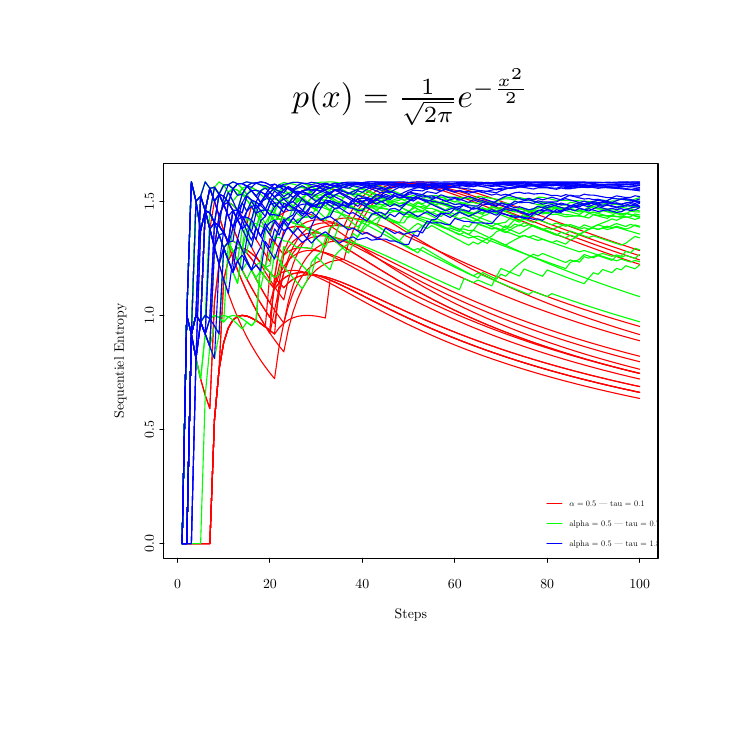
\begin{tikzpicture}[x=1pt,y=1pt]
\definecolor{fillColor}{RGB}{255,255,255}
\path[use as bounding box,fill=fillColor,fill opacity=0.00] (0,0) rectangle (252.94,252.94);
\begin{scope}
\path[clip] ( 49.20, 61.20) rectangle (227.75,203.75);
\definecolor{drawColor}{RGB}{255,0,0}

\path[draw=drawColor,line width= 0.4pt,line join=round,line cap=round] ( 55.81, 66.48) --
	( 57.48, 66.48) --
	( 59.15,142.23) --
	( 60.82,148.97) --
	( 62.49,146.57) --
	( 64.16,186.85) --
	( 65.83,194.89) --
	( 67.50,195.27) --
	( 69.17,192.73) --
	( 70.84,189.02) --
	( 72.51,184.89) --
	( 74.18,180.68) --
	( 75.85,176.58) --
	( 77.52,172.65) --
	( 79.19,168.93) --
	( 80.86,165.42) --
	( 82.53,162.13) --
	( 84.20,159.04) --
	( 85.87,156.15) --
	( 87.54,153.43) --
	( 89.21,150.87) --
	( 90.88,158.71) --
	( 92.55,164.35) --
	( 94.22,168.48) --
	( 95.89,171.51) --
	( 97.56,173.73) --
	( 99.23,175.33) --
	(100.90,176.43) --
	(102.57,177.15) --
	(104.24,177.56) --
	(105.91,177.72) --
	(107.58,177.69) --
	(109.25,177.49) --
	(110.92,177.15) --
	(112.59,176.71) --
	(114.26,176.18) --
	(115.93,175.58) --
	(117.60,174.92) --
	(119.27,174.22) --
	(120.94,173.48) --
	(122.61,172.71) --
	(124.28,171.91) --
	(125.95,171.10) --
	(127.62,170.28) --
	(129.29,169.44) --
	(130.96,168.60) --
	(132.63,167.76) --
	(134.30,166.92) --
	(135.97,166.07) --
	(137.64,165.23) --
	(139.31,164.40) --
	(140.98,163.57) --
	(142.65,162.75) --
	(144.32,161.93) --
	(145.99,161.12) --
	(147.66,160.32) --
	(149.33,159.53) --
	(151.00,158.75) --
	(152.67,157.98) --
	(154.34,157.22) --
	(156.01,156.47) --
	(157.68,155.72) --
	(159.35,154.99) --
	(161.02,154.27) --
	(162.69,153.56) --
	(164.36,152.86) --
	(166.03,152.17) --
	(167.70,151.48) --
	(169.37,150.81) --
	(171.04,150.15) --
	(172.71,149.50) --
	(174.38,148.86) --
	(176.05,148.22) --
	(177.71,147.60) --
	(179.38,146.99) --
	(181.05,146.38) --
	(182.72,145.78) --
	(184.39,145.20) --
	(186.06,144.62) --
	(187.73,144.05) --
	(189.40,143.48) --
	(191.07,142.93) --
	(192.74,142.38) --
	(194.41,141.85) --
	(196.08,141.32) --
	(197.75,140.79) --
	(199.42,140.28) --
	(201.09,139.77) --
	(202.76,139.27) --
	(204.43,138.78) --
	(206.10,138.29) --
	(207.77,137.81) --
	(209.44,137.34) --
	(211.11,136.87) --
	(212.78,136.41) --
	(214.45,135.96) --
	(216.12,135.51) --
	(217.79,135.07) --
	(219.46,134.64) --
	(221.13,134.21);
\end{scope}
\begin{scope}
\path[clip] (  0.00,  0.00) rectangle (252.94,252.94);
\definecolor{drawColor}{RGB}{0,0,0}

\path[draw=drawColor,line width= 0.4pt,line join=round,line cap=round] ( 54.14, 61.20) -- (221.13, 61.20);

\path[draw=drawColor,line width= 0.4pt,line join=round,line cap=round] ( 54.14, 61.20) -- ( 54.14, 59.77);

\path[draw=drawColor,line width= 0.4pt,line join=round,line cap=round] ( 87.54, 61.20) -- ( 87.54, 59.77);

\path[draw=drawColor,line width= 0.4pt,line join=round,line cap=round] (120.94, 61.20) -- (120.94, 59.77);

\path[draw=drawColor,line width= 0.4pt,line join=round,line cap=round] (154.34, 61.20) -- (154.34, 59.77);

\path[draw=drawColor,line width= 0.4pt,line join=round,line cap=round] (187.73, 61.20) -- (187.73, 59.77);

\path[draw=drawColor,line width= 0.4pt,line join=round,line cap=round] (221.13, 61.20) -- (221.13, 59.77);

\node[text=drawColor,anchor=base,inner sep=0pt, outer sep=0pt, scale=  0.50] at ( 54.14, 50.40) {0};

\node[text=drawColor,anchor=base,inner sep=0pt, outer sep=0pt, scale=  0.50] at ( 87.54, 50.40) {20};

\node[text=drawColor,anchor=base,inner sep=0pt, outer sep=0pt, scale=  0.50] at (120.94, 50.40) {40};

\node[text=drawColor,anchor=base,inner sep=0pt, outer sep=0pt, scale=  0.50] at (154.34, 50.40) {60};

\node[text=drawColor,anchor=base,inner sep=0pt, outer sep=0pt, scale=  0.50] at (187.73, 50.40) {80};

\node[text=drawColor,anchor=base,inner sep=0pt, outer sep=0pt, scale=  0.50] at (221.13, 50.40) {100};

\path[draw=drawColor,line width= 0.4pt,line join=round,line cap=round] ( 49.20, 66.48) -- ( 49.20,190.22);

\path[draw=drawColor,line width= 0.4pt,line join=round,line cap=round] ( 49.20, 66.48) -- ( 47.77, 66.48);

\path[draw=drawColor,line width= 0.4pt,line join=round,line cap=round] ( 49.20,107.73) -- ( 47.77,107.73);

\path[draw=drawColor,line width= 0.4pt,line join=round,line cap=round] ( 49.20,148.97) -- ( 47.77,148.97);

\path[draw=drawColor,line width= 0.4pt,line join=round,line cap=round] ( 49.20,190.22) -- ( 47.77,190.22);

\node[text=drawColor,rotate= 90.00,anchor=base,inner sep=0pt, outer sep=0pt, scale=  0.50] at ( 45.60, 66.48) {0.0};

\node[text=drawColor,rotate= 90.00,anchor=base,inner sep=0pt, outer sep=0pt, scale=  0.50] at ( 45.60,107.73) {0.5};

\node[text=drawColor,rotate= 90.00,anchor=base,inner sep=0pt, outer sep=0pt, scale=  0.50] at ( 45.60,148.97) {1.0};

\node[text=drawColor,rotate= 90.00,anchor=base,inner sep=0pt, outer sep=0pt, scale=  0.50] at ( 45.60,190.22) {1.5};

\path[draw=drawColor,line width= 0.4pt,line join=round,line cap=round] ( 49.20, 61.20) --
	(227.75, 61.20) --
	(227.75,203.75) --
	( 49.20,203.75) --
	( 49.20, 61.20);
\end{scope}
\begin{scope}
\path[clip] (  0.00,  0.00) rectangle (252.94,252.94);
\definecolor{drawColor}{RGB}{0,0,0}

\node[text=drawColor,anchor=base,inner sep=0pt, outer sep=0pt, scale=  0.50] at (138.47, 39.60) {Steps};

\node[text=drawColor,rotate= 90.00,anchor=base,inner sep=0pt, outer sep=0pt, scale=  0.50] at ( 34.80,132.47) {Sequentiel Entropy};
\end{scope}
\begin{scope}
\path[clip] ( 49.20, 61.20) rectangle (227.75,203.75);
\definecolor{drawColor}{RGB}{255,0,0}

\path[draw=drawColor,line width= 0.4pt,line join=round,line cap=round] ( 55.81, 66.48) --
	( 57.48, 66.48) --
	( 59.15,142.23) --
	( 60.82,148.97) --
	( 62.49,146.57) --
	( 64.16,142.23) --
	( 65.83,137.68) --
	( 67.50,173.62) --
	( 69.17,184.90) --
	( 70.84,189.02) --
	( 72.51,189.80) --
	( 74.18,188.84) --
	( 75.85,186.96) --
	( 77.52,184.57) --
	( 79.19,181.93) --
	( 80.86,188.34) --
	( 82.53,185.82) --
	( 84.20,183.23) --
	( 85.87,180.63) --
	( 87.54,178.07) --
	( 89.21,182.79) --
	( 90.88,184.89) --
	( 92.55,186.17) --
	( 94.22,186.85) --
	( 95.89,187.07) --
	( 97.56,186.96) --
	( 99.23,186.58) --
	(100.90,185.99) --
	(102.57,185.26) --
	(104.24,184.40) --
	(105.91,183.45) --
	(107.58,182.43) --
	(109.25,181.36) --
	(110.92,180.26) --
	(112.59,179.13) --
	(114.26,177.98) --
	(115.93,176.82) --
	(117.60,175.66) --
	(119.27,174.50) --
	(120.94,173.34) --
	(122.61,172.20) --
	(124.28,171.06) --
	(125.95,169.93) --
	(127.62,168.82) --
	(129.29,167.73) --
	(130.96,166.65) --
	(132.63,165.58) --
	(134.30,164.54) --
	(135.97,163.51) --
	(137.64,162.50) --
	(139.31,161.50) --
	(140.98,160.53) --
	(142.65,159.57) --
	(144.32,158.63) --
	(145.99,157.71) --
	(147.66,156.80) --
	(149.33,155.91) --
	(151.00,155.04) --
	(152.67,154.18) --
	(154.34,153.34) --
	(156.01,152.52) --
	(157.68,151.71) --
	(159.35,150.91) --
	(161.02,150.13) --
	(162.69,149.37) --
	(164.36,148.62) --
	(166.03,147.88) --
	(167.70,147.16) --
	(169.37,146.45) --
	(171.04,145.75) --
	(172.71,145.06) --
	(174.38,144.39) --
	(176.05,143.73) --
	(177.71,143.08) --
	(179.38,142.44) --
	(181.05,141.82) --
	(182.72,141.20) --
	(184.39,140.60) --
	(186.06,140.00) --
	(187.73,139.42) --
	(189.40,138.84) --
	(191.07,138.28) --
	(192.74,137.72) --
	(194.41,137.17) --
	(196.08,136.64) --
	(197.75,136.11) --
	(199.42,135.59) --
	(201.09,135.07) --
	(202.76,134.57) --
	(204.43,134.07) --
	(206.10,133.59) --
	(207.77,133.11) --
	(209.44,132.63) --
	(211.11,132.17) --
	(212.78,131.71) --
	(214.45,131.25) --
	(216.12,130.81) --
	(217.79,130.37) --
	(219.46,129.94) --
	(221.13,129.51);

\path[draw=drawColor,line width= 0.4pt,line join=round,line cap=round] ( 55.81, 66.48) --
	( 57.48,148.97) --
	( 59.15,142.23) --
	( 60.82,133.40) --
	( 62.49,126.03) --
	( 64.16,120.10) --
	( 65.83,115.29) --
	( 67.50,154.03) --
	( 69.17,167.48) --
	( 70.84,173.34) --
	( 72.51,175.55) --
	( 74.18,175.78) --
	( 75.85,174.90) --
	( 77.52,173.37) --
	( 79.19,171.48) --
	( 80.86,169.39) --
	( 82.53,167.21) --
	( 84.20,164.99) --
	( 85.87,162.78) --
	( 87.54,160.61) --
	( 89.21,158.50) --
	( 90.88,160.79) --
	( 92.55,162.38) --
	( 94.22,163.43) --
	( 95.89,164.06) --
	( 97.56,164.37) --
	( 99.23,164.43) --
	(100.90,164.28) --
	(102.57,163.98) --
	(104.24,163.55) --
	(105.91,163.01) --
	(107.58,162.40) --
	(109.25,161.73) --
	(110.92,161.01) --
	(112.59,160.24) --
	(114.26,159.46) --
	(115.93,158.65) --
	(117.60,157.82) --
	(119.27,156.98) --
	(120.94,156.14) --
	(122.61,155.30) --
	(124.28,154.46) --
	(125.95,153.61) --
	(127.62,152.78) --
	(129.29,151.95) --
	(130.96,151.12) --
	(132.63,150.31) --
	(134.30,149.50) --
	(135.97,148.71) --
	(137.64,147.92) --
	(139.31,147.15) --
	(140.98,146.39) --
	(142.65,145.63) --
	(144.32,144.89) --
	(145.99,144.16) --
	(147.66,143.45) --
	(149.33,142.74) --
	(151.00,142.05) --
	(152.67,141.36) --
	(154.34,140.69) --
	(156.01,140.03) --
	(157.68,139.38) --
	(159.35,138.74) --
	(161.02,138.11) --
	(162.69,137.50) --
	(164.36,136.89) --
	(166.03,136.29) --
	(167.70,135.71) --
	(169.37,135.13) --
	(171.04,134.56) --
	(172.71,134.00) --
	(174.38,133.45) --
	(176.05,132.91) --
	(177.71,132.38) --
	(179.38,131.86) --
	(181.05,131.35) --
	(182.72,130.84) --
	(184.39,130.35) --
	(186.06,129.86) --
	(187.73,129.38) --
	(189.40,128.90) --
	(191.07,128.44) --
	(192.74,127.98) --
	(194.41,127.53) --
	(196.08,127.08) --
	(197.75,126.64) --
	(199.42,126.21) --
	(201.09,125.79) --
	(202.76,125.37) --
	(204.43,124.96) --
	(206.10,124.55) --
	(207.77,124.15) --
	(209.44,123.76) --
	(211.11,123.37) --
	(212.78,122.99) --
	(214.45,122.61) --
	(216.12,122.24) --
	(217.79,121.88) --
	(219.46,121.51) --
	(221.13,121.16);

\path[draw=drawColor,line width= 0.4pt,line join=round,line cap=round] ( 55.81, 66.48) --
	( 57.48, 66.48) --
	( 59.15,142.23) --
	( 60.82,148.97) --
	( 62.49,146.57) --
	( 64.16,186.85) --
	( 65.83,194.89) --
	( 67.50,190.22) --
	( 69.17,184.90) --
	( 70.84,179.57) --
	( 72.51,174.49) --
	( 74.18,169.73) --
	( 75.85,165.32) --
	( 77.52,161.25) --
	( 79.19,157.49) --
	( 80.86,154.03) --
	( 82.53,150.82) --
	( 84.20,147.85) --
	( 85.87,145.09) --
	( 87.54,142.53) --
	( 89.21,140.14) --
	( 90.88,137.91) --
	( 92.55,135.81) --
	( 94.22,144.07) --
	( 95.89,150.24) --
	( 97.56,154.97) --
	( 99.23,158.63) --
	(100.90,161.47) --
	(102.57,163.68) --
	(104.24,165.38) --
	(105.91,166.67) --
	(107.58,167.62) --
	(109.25,168.31) --
	(110.92,168.76) --
	(112.59,169.03) --
	(114.26,169.14) --
	(115.93,175.01) --
	(117.60,179.60) --
	(119.27,183.25) --
	(120.94,186.20) --
	(122.61,188.60) --
	(124.28,190.54) --
	(125.95,192.11) --
	(127.62,193.37) --
	(129.29,194.37) --
	(130.96,195.15) --
	(132.63,195.74) --
	(134.30,196.16) --
	(135.97,196.45) --
	(137.64,196.62) --
	(139.31,196.67) --
	(140.98,196.64) --
	(142.65,196.53) --
	(144.32,196.34) --
	(145.99,196.10) --
	(147.66,195.80) --
	(149.33,195.45) --
	(151.00,195.07) --
	(152.67,194.64) --
	(154.34,194.19) --
	(156.01,193.70) --
	(157.68,193.20) --
	(159.35,192.67) --
	(161.02,192.12) --
	(162.69,191.56) --
	(164.36,190.99) --
	(166.03,190.40) --
	(167.70,189.80) --
	(169.37,189.20) --
	(171.04,188.59) --
	(172.71,187.97) --
	(174.38,187.35) --
	(176.05,186.73) --
	(177.71,186.10) --
	(179.38,185.47) --
	(181.05,184.84) --
	(182.72,184.22) --
	(184.39,183.59) --
	(186.06,182.96) --
	(187.73,182.33) --
	(189.40,181.71) --
	(191.07,181.09) --
	(192.74,180.47) --
	(194.41,179.85) --
	(196.08,179.24) --
	(197.75,178.63) --
	(199.42,178.03) --
	(201.09,177.42) --
	(202.76,176.82) --
	(204.43,176.23) --
	(206.10,175.64) --
	(207.77,175.05) --
	(209.44,174.47) --
	(211.11,173.90) --
	(212.78,173.33) --
	(214.45,172.76) --
	(216.12,172.19) --
	(217.79,171.64) --
	(219.46,171.08) --
	(221.13,170.54);

\path[draw=drawColor,line width= 0.4pt,line join=round,line cap=round] ( 55.81, 66.48) --
	( 57.48, 66.48) --
	( 59.15, 66.48) --
	( 60.82, 66.48) --
	( 62.49, 66.48) --
	( 64.16, 66.48) --
	( 65.83, 66.48) --
	( 67.50,111.32) --
	( 69.17,129.52) --
	( 70.84,139.18) --
	( 72.51,144.49) --
	( 74.18,147.31) --
	( 75.85,148.62) --
	( 77.52,148.97) --
	( 79.19,148.71) --
	( 80.86,148.04) --
	( 82.53,147.11) --
	( 84.20,146.01) --
	( 85.87,144.80) --
	( 87.54,164.51) --
	( 89.21,162.65) --
	( 90.88,163.98) --
	( 92.55,164.78) --
	( 94.22,165.17) --
	( 95.89,165.26) --
	( 97.56,165.11) --
	( 99.23,164.77) --
	(100.90,164.28) --
	(102.57,163.68) --
	(104.24,163.00) --
	(105.91,162.24) --
	(107.58,161.44) --
	(109.25,160.59) --
	(110.92,159.72) --
	(112.59,158.82) --
	(114.26,157.92) --
	(115.93,157.00) --
	(117.60,156.08) --
	(119.27,155.17) --
	(120.94,154.25) --
	(122.61,153.34) --
	(124.28,152.44) --
	(125.95,151.55) --
	(127.62,150.66) --
	(129.29,149.79) --
	(130.96,148.93) --
	(132.63,148.08) --
	(134.30,147.25) --
	(135.97,146.43) --
	(137.64,145.62) --
	(139.31,144.83) --
	(140.98,144.05) --
	(142.65,143.28) --
	(144.32,142.53) --
	(145.99,141.79) --
	(147.66,141.06) --
	(149.33,140.34) --
	(151.00,139.64) --
	(152.67,138.96) --
	(154.34,138.28) --
	(156.01,137.62) --
	(157.68,136.96) --
	(159.35,136.32) --
	(161.02,135.70) --
	(162.69,135.08) --
	(164.36,134.47) --
	(166.03,133.88) --
	(167.70,133.29) --
	(169.37,132.72) --
	(171.04,132.16) --
	(172.71,131.60) --
	(174.38,131.06) --
	(176.05,130.52) --
	(177.71,130.00) --
	(179.38,129.48) --
	(181.05,128.97) --
	(182.72,128.47) --
	(184.39,127.98) --
	(186.06,127.50) --
	(187.73,127.03) --
	(189.40,126.56) --
	(191.07,126.10) --
	(192.74,125.65) --
	(194.41,125.20) --
	(196.08,124.77) --
	(197.75,124.34) --
	(199.42,123.91) --
	(201.09,123.50) --
	(202.76,123.09) --
	(204.43,122.68) --
	(206.10,122.28) --
	(207.77,121.89) --
	(209.44,121.51) --
	(211.11,121.13) --
	(212.78,120.75) --
	(214.45,120.38) --
	(216.12,120.02) --
	(217.79,119.66) --
	(219.46,119.31) --
	(221.13,118.96);

\path[draw=drawColor,line width= 0.4pt,line join=round,line cap=round] ( 55.81, 66.48) --
	( 57.48, 66.48) --
	( 59.15, 66.48) --
	( 60.82, 66.48) --
	( 62.49, 66.48) --
	( 64.16, 66.48) --
	( 65.83, 66.48) --
	( 67.50,111.32) --
	( 69.17,129.52) --
	( 70.84,139.18) --
	( 72.51,144.49) --
	( 74.18,147.31) --
	( 75.85,148.62) --
	( 77.52,148.97) --
	( 79.19,148.71) --
	( 80.86,148.04) --
	( 82.53,147.11) --
	( 84.20,146.01) --
	( 85.87,144.80) --
	( 87.54,143.53) --
	( 89.21,162.65) --
	( 90.88,160.79) --
	( 92.55,158.97) --
	( 94.22,160.78) --
	( 95.89,162.05) --
	( 97.56,162.90) --
	( 99.23,163.41) --
	(100.90,163.65) --
	(102.57,163.68) --
	(104.24,163.55) --
	(105.91,163.27) --
	(107.58,162.88) --
	(109.25,162.41) --
	(110.92,161.86) --
	(112.59,161.25) --
	(114.26,160.60) --
	(115.93,159.91) --
	(117.60,159.20) --
	(119.27,158.46) --
	(120.94,157.70) --
	(122.61,156.94) --
	(124.28,156.16) --
	(125.95,155.39) --
	(127.62,154.61) --
	(129.29,153.83) --
	(130.96,153.05) --
	(132.63,152.27) --
	(134.30,151.51) --
	(135.97,150.74) --
	(137.64,149.99) --
	(139.31,149.24) --
	(140.98,148.50) --
	(142.65,147.77) --
	(144.32,147.04) --
	(145.99,146.33) --
	(147.66,145.63) --
	(149.33,144.94) --
	(151.00,144.25) --
	(152.67,143.58) --
	(154.34,142.91) --
	(156.01,142.26) --
	(157.68,141.62) --
	(159.35,140.98) --
	(161.02,140.36) --
	(162.69,139.74) --
	(164.36,139.14) --
	(166.03,138.54) --
	(167.70,137.96) --
	(169.37,137.38) --
	(171.04,136.81) --
	(172.71,136.25) --
	(174.38,135.70) --
	(176.05,135.16) --
	(177.71,134.63) --
	(179.38,134.10) --
	(181.05,133.59) --
	(182.72,133.08) --
	(184.39,132.58) --
	(186.06,132.08) --
	(187.73,131.60) --
	(189.40,131.12) --
	(191.07,130.65) --
	(192.74,130.18) --
	(194.41,129.73) --
	(196.08,129.28) --
	(197.75,128.83) --
	(199.42,128.40) --
	(201.09,127.97) --
	(202.76,127.54) --
	(204.43,127.12) --
	(206.10,126.71) --
	(207.77,126.31) --
	(209.44,125.90) --
	(211.11,125.51) --
	(212.78,125.12) --
	(214.45,124.74) --
	(216.12,124.36) --
	(217.79,123.99) --
	(219.46,123.62) --
	(221.13,123.26);

\path[draw=drawColor,line width= 0.4pt,line join=round,line cap=round] ( 55.81, 66.48) --
	( 57.48, 66.48) --
	( 59.15,142.23) --
	( 60.82,190.22) --
	( 62.49,192.03) --
	( 64.16,186.85) --
	( 65.83,180.22) --
	( 67.50,182.43) --
	( 69.17,181.32) --
	( 70.84,178.75) --
	( 72.51,175.55) --
	( 74.18,172.12) --
	( 75.85,168.68) --
	( 77.52,165.31) --
	( 79.19,162.08) --
	( 80.86,159.01) --
	( 82.53,156.09) --
	( 84.20,153.34) --
	( 85.87,150.74) --
	( 87.54,148.29) --
	( 89.21,145.98) --
	( 90.88,156.87) --
	( 92.55,164.35) --
	( 94.22,169.73) --
	( 95.89,173.67) --
	( 97.56,176.58) --
	( 99.23,178.70) --
	(100.90,180.22) --
	(102.57,181.26) --
	(104.24,181.93) --
	(105.91,182.30) --
	(107.58,182.43) --
	(109.25,182.37) --
	(110.92,182.14) --
	(112.59,181.78) --
	(114.26,181.32) --
	(115.93,180.77) --
	(117.60,180.33) --
	(119.27,179.82) --
	(120.94,183.46) --
	(122.61,186.40) --
	(124.28,188.80) --
	(125.95,190.76) --
	(127.62,192.35) --
	(129.29,193.64) --
	(130.96,194.67) --
	(132.63,195.48) --
	(134.30,196.11) --
	(135.97,196.57) --
	(137.64,196.89) --
	(139.31,197.09) --
	(140.98,197.18) --
	(142.65,197.18) --
	(144.32,197.10) --
	(145.99,196.95) --
	(147.66,196.74) --
	(149.33,196.47) --
	(151.00,196.16) --
	(152.67,195.80) --
	(154.34,195.40) --
	(156.01,194.97) --
	(157.68,194.52) --
	(159.35,194.04) --
	(161.02,193.53) --
	(162.69,193.01) --
	(164.36,192.47) --
	(166.03,191.92) --
	(167.70,191.35) --
	(169.37,190.78) --
	(171.04,190.19) --
	(172.71,189.60) --
	(174.38,189.00) --
	(176.05,188.40) --
	(177.71,187.79) --
	(179.38,187.18) --
	(181.05,186.57) --
	(182.72,185.95) --
	(184.39,185.34) --
	(186.06,184.72) --
	(187.73,184.11) --
	(189.40,183.49) --
	(191.07,182.88) --
	(192.74,182.27) --
	(194.41,181.66) --
	(196.08,181.05) --
	(197.75,180.45) --
	(199.42,179.85) --
	(201.09,179.25) --
	(202.76,178.66) --
	(204.43,178.07) --
	(206.10,177.48) --
	(207.77,176.90) --
	(209.44,176.32) --
	(211.11,175.75) --
	(212.78,175.17) --
	(214.45,174.61) --
	(216.12,174.05) --
	(217.79,173.49) --
	(219.46,172.94) --
	(221.13,172.39);

\path[draw=drawColor,line width= 0.4pt,line join=round,line cap=round] ( 55.81, 66.48) --
	( 57.48, 66.48) --
	( 59.15, 66.48) --
	( 60.82, 66.48) --
	( 62.49, 66.48) --
	( 64.16, 66.48) --
	( 65.83, 66.48) --
	( 67.50,111.32) --
	( 69.17,129.52) --
	( 70.84,139.18) --
	( 72.51,144.49) --
	( 74.18,147.31) --
	( 75.85,148.62) --
	( 77.52,148.97) --
	( 79.19,148.71) --
	( 80.86,148.04) --
	( 82.53,147.11) --
	( 84.20,168.16) --
	( 85.87,166.36) --
	( 87.54,176.74) --
	( 89.21,174.77) --
	( 90.88,181.52) --
	( 92.55,186.17) --
	( 94.22,189.39) --
	( 95.89,191.59) --
	( 97.56,193.04) --
	( 99.23,193.92) --
	(100.90,194.89) --
	(102.57,195.43) --
	(104.24,195.63) --
	(105.91,195.56) --
	(107.58,195.27) --
	(109.25,194.82) --
	(110.92,194.22) --
	(112.59,193.52) --
	(114.26,192.73) --
	(115.93,191.87) --
	(117.60,190.96) --
	(119.27,190.01) --
	(120.94,189.02) --
	(122.61,188.01) --
	(124.28,186.98) --
	(125.95,185.93) --
	(127.62,184.89) --
	(129.29,183.83) --
	(130.96,182.78) --
	(132.63,181.73) --
	(134.30,180.68) --
	(135.97,179.64) --
	(137.64,178.61) --
	(139.31,177.59) --
	(140.98,176.58) --
	(142.65,175.58) --
	(144.32,174.59) --
	(145.99,173.61) --
	(147.66,172.65) --
	(149.33,171.70) --
	(151.00,170.76) --
	(152.67,169.84) --
	(154.34,168.93) --
	(156.01,168.03) --
	(157.68,167.15) --
	(159.35,166.28) --
	(161.02,165.42) --
	(162.69,164.58) --
	(164.36,163.75) --
	(166.03,162.94) --
	(167.70,162.13) --
	(169.37,161.34) --
	(171.04,160.56) --
	(172.71,159.80) --
	(174.38,159.04) --
	(176.05,158.30) --
	(177.71,157.57) --
	(179.38,156.85) --
	(181.05,156.15) --
	(182.72,155.45) --
	(184.39,154.77) --
	(186.06,154.09) --
	(187.73,153.43) --
	(189.40,152.77) --
	(191.07,152.13) --
	(192.74,151.50) --
	(194.41,150.87) --
	(196.08,150.26) --
	(197.75,149.65) --
	(199.42,149.05) --
	(201.09,148.47) --
	(202.76,147.89) --
	(204.43,147.32) --
	(206.10,146.76) --
	(207.77,146.20) --
	(209.44,145.66) --
	(211.11,145.12) --
	(212.78,144.59) --
	(214.45,144.07) --
	(216.12,143.55) --
	(217.79,143.05) --
	(219.46,142.54) --
	(221.13,142.05);

\path[draw=drawColor,line width= 0.4pt,line join=round,line cap=round] ( 55.81, 66.48) --
	( 57.48, 66.48) --
	( 59.15,142.23) --
	( 60.82,190.22) --
	( 62.49,192.03) --
	( 64.16,186.85) --
	( 65.83,180.22) --
	( 67.50,182.43) --
	( 69.17,181.32) --
	( 70.84,178.75) --
	( 72.51,175.55) --
	( 74.18,172.12) --
	( 75.85,168.68) --
	( 77.52,165.31) --
	( 79.19,162.08) --
	( 80.86,159.01) --
	( 82.53,156.09) --
	( 84.20,153.34) --
	( 85.87,150.74) --
	( 87.54,148.29) --
	( 89.21,159.32) --
	( 90.88,163.57) --
	( 92.55,166.65) --
	( 94.22,168.85) --
	( 95.89,170.40) --
	( 97.56,171.43) --
	( 99.23,172.07) --
	(100.90,172.39) --
	(102.57,172.46) --
	(104.24,172.34) --
	(105.91,172.05) --
	(107.58,171.64) --
	(109.25,171.12) --
	(110.92,170.52) --
	(112.59,169.86) --
	(114.26,169.14) --
	(115.93,168.38) --
	(117.60,167.59) --
	(119.27,166.78) --
	(120.94,165.95) --
	(122.61,165.10) --
	(124.28,164.25) --
	(125.95,163.39) --
	(127.62,162.52) --
	(129.29,161.66) --
	(130.96,160.80) --
	(132.63,159.95) --
	(134.30,159.10) --
	(135.97,158.26) --
	(137.64,157.43) --
	(139.31,156.60) --
	(140.98,155.78) --
	(142.65,154.98) --
	(144.32,154.18) --
	(145.99,153.40) --
	(147.66,152.62) --
	(149.33,151.86) --
	(151.00,151.10) --
	(152.67,150.36) --
	(154.34,149.63) --
	(156.01,148.91) --
	(157.68,148.20) --
	(159.35,147.51) --
	(161.02,146.82) --
	(162.69,146.14) --
	(164.36,145.48) --
	(166.03,144.82) --
	(167.70,144.18) --
	(169.37,143.55) --
	(171.04,142.92) --
	(172.71,142.31) --
	(174.38,141.70) --
	(176.05,141.11) --
	(177.71,140.52) --
	(179.38,139.95) --
	(181.05,139.38) --
	(182.72,138.82) --
	(184.39,138.27) --
	(186.06,137.73) --
	(187.73,137.20) --
	(189.40,136.67) --
	(191.07,136.16) --
	(192.74,135.65) --
	(194.41,135.15) --
	(196.08,134.65) --
	(197.75,134.17) --
	(199.42,133.69) --
	(201.09,133.22) --
	(202.76,132.75) --
	(204.43,132.29) --
	(206.10,131.84) --
	(207.77,131.40) --
	(209.44,130.96) --
	(211.11,130.53) --
	(212.78,130.10) --
	(214.45,129.68) --
	(216.12,129.27) --
	(217.79,128.86) --
	(219.46,128.46) --
	(221.13,128.06);

\path[draw=drawColor,line width= 0.4pt,line join=round,line cap=round] ( 55.81, 66.48) --
	( 57.48, 66.48) --
	( 59.15, 66.48) --
	( 60.82, 66.48) --
	( 62.49, 66.48) --
	( 64.16, 66.48) --
	( 65.83, 66.48) --
	( 67.50,111.32) --
	( 69.17,129.52) --
	( 70.84,139.18) --
	( 72.51,144.49) --
	( 74.18,147.31) --
	( 75.85,148.62) --
	( 77.52,148.97) --
	( 79.19,148.71) --
	( 80.86,148.04) --
	( 82.53,147.11) --
	( 84.20,146.01) --
	( 85.87,144.80) --
	( 87.54,143.53) --
	( 89.21,162.65) --
	( 90.88,160.79) --
	( 92.55,158.97) --
	( 94.22,160.78) --
	( 95.89,162.05) --
	( 97.56,162.90) --
	( 99.23,163.41) --
	(100.90,163.65) --
	(102.57,163.68) --
	(104.24,163.55) --
	(105.91,163.27) --
	(107.58,162.88) --
	(109.25,162.41) --
	(110.92,161.86) --
	(112.59,161.25) --
	(114.26,160.60) --
	(115.93,159.91) --
	(117.60,159.20) --
	(119.27,158.46) --
	(120.94,157.70) --
	(122.61,156.94) --
	(124.28,156.16) --
	(125.95,155.39) --
	(127.62,154.61) --
	(129.29,153.83) --
	(130.96,153.05) --
	(132.63,152.27) --
	(134.30,151.51) --
	(135.97,150.74) --
	(137.64,149.99) --
	(139.31,149.24) --
	(140.98,148.50) --
	(142.65,147.77) --
	(144.32,147.04) --
	(145.99,146.33) --
	(147.66,145.63) --
	(149.33,144.94) --
	(151.00,144.25) --
	(152.67,143.58) --
	(154.34,142.91) --
	(156.01,142.26) --
	(157.68,141.62) --
	(159.35,140.98) --
	(161.02,140.36) --
	(162.69,139.74) --
	(164.36,139.14) --
	(166.03,138.54) --
	(167.70,137.96) --
	(169.37,137.38) --
	(171.04,136.81) --
	(172.71,136.25) --
	(174.38,135.70) --
	(176.05,135.16) --
	(177.71,134.63) --
	(179.38,134.10) --
	(181.05,133.59) --
	(182.72,133.08) --
	(184.39,132.58) --
	(186.06,132.08) --
	(187.73,131.60) --
	(189.40,131.12) --
	(191.07,130.65) --
	(192.74,130.18) --
	(194.41,129.73) --
	(196.08,129.28) --
	(197.75,128.83) --
	(199.42,128.40) --
	(201.09,127.97) --
	(202.76,127.54) --
	(204.43,127.12) --
	(206.10,126.71) --
	(207.77,126.31) --
	(209.44,125.90) --
	(211.11,125.51) --
	(212.78,125.12) --
	(214.45,124.74) --
	(216.12,124.36) --
	(217.79,123.99) --
	(219.46,123.62) --
	(221.13,123.26);

\path[draw=drawColor,line width= 0.4pt,line join=round,line cap=round] ( 55.81, 66.48) --
	( 57.48, 66.48) --
	( 59.15,142.23) --
	( 60.82,148.97) --
	( 62.49,192.03) --
	( 64.16,186.85) --
	( 65.83,180.22) --
	( 67.50,173.62) --
	( 69.17,167.48) --
	( 70.84,161.90) --
	( 72.51,156.87) --
	( 74.18,152.34) --
	( 75.85,148.25) --
	( 77.52,144.55) --
	( 79.19,141.18) --
	( 80.86,138.11) --
	( 82.53,135.31) --
	( 84.20,132.73) --
	( 85.87,130.35) --
	( 87.54,128.15) --
	( 89.21,126.11) --
	( 90.88,137.91) --
	( 92.55,146.20) --
	( 94.22,152.34) --
	( 95.89,156.98) --
	( 97.56,160.53) --
	( 99.23,163.24) --
	(100.90,165.31) --
	(102.57,166.87) --
	(104.24,168.02) --
	(105.91,168.84) --
	(107.58,175.09) --
	(109.25,179.85) --
	(110.92,183.55) --
	(112.59,183.94) --
	(114.26,184.13) --
	(115.93,184.15) --
	(117.60,184.03) --
	(119.27,183.79) --
	(120.94,183.46) --
	(122.61,183.04) --
	(124.28,182.55) --
	(125.95,182.01) --
	(127.62,181.42) --
	(129.29,180.79) --
	(130.96,180.13) --
	(132.63,179.44) --
	(134.30,178.73) --
	(135.97,178.00) --
	(137.64,177.25) --
	(139.31,176.50) --
	(140.98,175.74) --
	(142.65,174.97) --
	(144.32,174.20) --
	(145.99,173.43) --
	(147.66,172.66) --
	(149.33,171.88) --
	(151.00,171.11) --
	(152.67,170.35) --
	(154.34,169.59) --
	(156.01,168.83) --
	(157.68,168.08) --
	(159.35,167.33) --
	(161.02,166.59) --
	(162.69,165.86) --
	(164.36,165.13) --
	(166.03,164.42) --
	(167.70,163.70) --
	(169.37,163.00) --
	(171.04,162.31) --
	(172.71,161.62) --
	(174.38,160.94) --
	(176.05,160.27) --
	(177.71,159.60) --
	(179.38,158.95) --
	(181.05,158.30) --
	(182.72,157.66) --
	(184.39,157.03) --
	(186.06,156.40) --
	(187.73,155.79) --
	(189.40,155.18) --
	(191.07,154.58) --
	(192.74,153.99) --
	(194.41,153.40) --
	(196.08,152.82) --
	(197.75,152.25) --
	(199.42,151.69) --
	(201.09,151.13) --
	(202.76,150.59) --
	(204.43,150.04) --
	(206.10,149.51) --
	(207.77,148.98) --
	(209.44,148.46) --
	(211.11,147.94) --
	(212.78,147.44) --
	(214.45,146.94) --
	(216.12,146.44) --
	(217.79,145.95) --
	(219.46,145.47) --
	(221.13,144.99);

\path[draw=drawColor,line width= 0.4pt,line join=round,line cap=round] ( 55.81, 66.48) --
	( 57.48,148.97) --
	( 59.15,142.23) --
	( 60.82,133.40) --
	( 62.49,126.03) --
	( 64.16,120.10) --
	( 65.83,115.29) --
	( 67.50,154.03) --
	( 69.17,167.48) --
	( 70.84,173.34) --
	( 72.51,175.55) --
	( 74.18,175.78) --
	( 75.85,174.90) --
	( 77.52,173.37) --
	( 79.19,171.48) --
	( 80.86,169.39) --
	( 82.53,167.21) --
	( 84.20,164.99) --
	( 85.87,162.78) --
	( 87.54,160.61) --
	( 89.21,158.50) --
	( 90.88,160.79) --
	( 92.55,162.38) --
	( 94.22,163.43) --
	( 95.89,164.06) --
	( 97.56,164.37) --
	( 99.23,164.43) --
	(100.90,164.28) --
	(102.57,163.98) --
	(104.24,163.55) --
	(105.91,163.01) --
	(107.58,162.40) --
	(109.25,161.73) --
	(110.92,161.01) --
	(112.59,160.24) --
	(114.26,159.46) --
	(115.93,158.65) --
	(117.60,157.82) --
	(119.27,156.98) --
	(120.94,156.14) --
	(122.61,155.30) --
	(124.28,154.46) --
	(125.95,153.61) --
	(127.62,152.78) --
	(129.29,151.95) --
	(130.96,151.12) --
	(132.63,150.31) --
	(134.30,149.50) --
	(135.97,148.71) --
	(137.64,147.92) --
	(139.31,147.15) --
	(140.98,146.39) --
	(142.65,145.63) --
	(144.32,144.89) --
	(145.99,144.16) --
	(147.66,143.45) --
	(149.33,142.74) --
	(151.00,142.05) --
	(152.67,141.36) --
	(154.34,140.69) --
	(156.01,140.03) --
	(157.68,139.38) --
	(159.35,138.74) --
	(161.02,138.11) --
	(162.69,137.50) --
	(164.36,136.89) --
	(166.03,136.29) --
	(167.70,135.71) --
	(169.37,135.13) --
	(171.04,134.56) --
	(172.71,134.00) --
	(174.38,133.45) --
	(176.05,132.91) --
	(177.71,132.38) --
	(179.38,131.86) --
	(181.05,131.35) --
	(182.72,130.84) --
	(184.39,130.35) --
	(186.06,129.86) --
	(187.73,129.38) --
	(189.40,128.90) --
	(191.07,128.44) --
	(192.74,127.98) --
	(194.41,127.53) --
	(196.08,127.08) --
	(197.75,126.64) --
	(199.42,126.21) --
	(201.09,125.79) --
	(202.76,125.37) --
	(204.43,124.96) --
	(206.10,124.55) --
	(207.77,124.15) --
	(209.44,123.76) --
	(211.11,123.37) --
	(212.78,122.99) --
	(214.45,122.61) --
	(216.12,122.24) --
	(217.79,121.88) --
	(219.46,121.51) --
	(221.13,121.16);

\path[draw=drawColor,line width= 0.4pt,line join=round,line cap=round] ( 55.81, 66.48) --
	( 57.48, 66.48) --
	( 59.15, 66.48) --
	( 60.82, 66.48) --
	( 62.49, 66.48) --
	( 64.16, 66.48) --
	( 65.83, 66.48) --
	( 67.50,111.32) --
	( 69.17,129.52) --
	( 70.84,139.18) --
	( 72.51,144.49) --
	( 74.18,147.31) --
	( 75.85,148.62) --
	( 77.52,148.97) --
	( 79.19,148.71) --
	( 80.86,148.04) --
	( 82.53,147.11) --
	( 84.20,146.01) --
	( 85.87,144.80) --
	( 87.54,143.53) --
	( 89.21,142.23) --
	( 90.88,160.79) --
	( 92.55,170.80) --
	( 94.22,172.12) --
	( 95.89,172.94) --
	( 97.56,173.37) --
	( 99.23,173.49) --
	(100.90,173.37) --
	(102.57,173.07) --
	(104.24,172.62) --
	(105.91,172.05) --
	(107.58,171.39) --
	(109.25,170.66) --
	(110.92,169.87) --
	(112.59,169.03) --
	(114.26,168.16) --
	(115.93,167.27) --
	(117.60,166.36) --
	(119.27,165.44) --
	(120.94,164.51) --
	(122.61,163.58) --
	(124.28,162.65) --
	(125.95,161.72) --
	(127.62,160.79) --
	(129.29,159.88) --
	(130.96,158.97) --
	(132.63,158.07) --
	(134.30,157.18) --
	(135.97,156.30) --
	(137.64,155.43) --
	(139.31,154.58) --
	(140.98,153.73) --
	(142.65,152.90) --
	(144.32,152.09) --
	(145.99,151.28) --
	(147.66,150.49) --
	(149.33,149.71) --
	(151.00,148.95) --
	(152.67,148.19) --
	(154.34,147.45) --
	(156.01,146.72) --
	(157.68,146.01) --
	(159.35,145.30) --
	(161.02,144.61) --
	(162.69,143.93) --
	(164.36,143.26) --
	(166.03,142.61) --
	(167.70,141.96) --
	(169.37,141.33) --
	(171.04,140.70) --
	(172.71,140.09) --
	(174.38,139.48) --
	(176.05,138.89) --
	(177.71,138.31) --
	(179.38,137.73) --
	(181.05,137.17) --
	(182.72,136.61) --
	(184.39,136.07) --
	(186.06,135.53) --
	(187.73,135.00) --
	(189.40,134.48) --
	(191.07,133.97) --
	(192.74,133.46) --
	(194.41,132.97) --
	(196.08,132.48) --
	(197.75,132.00) --
	(199.42,131.53) --
	(201.09,131.06) --
	(202.76,130.60) --
	(204.43,130.15) --
	(206.10,129.70) --
	(207.77,129.26) --
	(209.44,128.83) --
	(211.11,128.41) --
	(212.78,127.99) --
	(214.45,127.57) --
	(216.12,127.17) --
	(217.79,126.76) --
	(219.46,126.37) --
	(221.13,125.98);

\path[draw=drawColor,line width= 0.4pt,line join=round,line cap=round] ( 55.81, 66.48) --
	( 57.48, 66.48) --
	( 59.15,142.23) --
	( 60.82,148.97) --
	( 62.49,146.57) --
	( 64.16,186.85) --
	( 65.83,194.89) --
	( 67.50,195.27) --
	( 69.17,192.73) --
	( 70.84,189.02) --
	( 72.51,184.89) --
	( 74.18,180.68) --
	( 75.85,176.58) --
	( 77.52,172.65) --
	( 79.19,168.93) --
	( 80.86,165.42) --
	( 82.53,162.13) --
	( 84.20,159.04) --
	( 85.87,156.15) --
	( 87.54,153.43) --
	( 89.21,159.32) --
	( 90.88,156.87) --
	( 92.55,154.55) --
	( 94.22,162.02) --
	( 95.89,167.48) --
	( 97.56,171.54) --
	( 99.23,174.59) --
	(100.90,176.86) --
	(102.57,178.54) --
	(104.24,179.74) --
	(105.91,180.57) --
	(107.58,181.09) --
	(109.25,181.36) --
	(110.92,181.44) --
	(112.59,181.34) --
	(114.26,181.11) --
	(115.93,180.77) --
	(117.60,180.33) --
	(119.27,179.82) --
	(120.94,179.24) --
	(122.61,178.62) --
	(124.28,177.94) --
	(125.95,177.24) --
	(127.62,176.50) --
	(129.29,175.75) --
	(130.96,174.97) --
	(132.63,174.19) --
	(134.30,173.39) --
	(135.97,172.59) --
	(137.64,171.78) --
	(139.31,170.97) --
	(140.98,170.16) --
	(142.65,169.35) --
	(144.32,168.54) --
	(145.99,167.74) --
	(147.66,166.94) --
	(149.33,166.15) --
	(151.00,165.36) --
	(152.67,164.59) --
	(154.34,163.81) --
	(156.01,163.05) --
	(157.68,162.29) --
	(159.35,161.55) --
	(161.02,160.81) --
	(162.69,160.08) --
	(164.36,159.36) --
	(166.03,158.64) --
	(167.70,157.94) --
	(169.37,157.25) --
	(171.04,156.56) --
	(172.71,155.89) --
	(174.38,155.22) --
	(176.05,154.56) --
	(177.71,153.91) --
	(179.38,153.27) --
	(181.05,152.64) --
	(182.72,152.02) --
	(184.39,151.40) --
	(186.06,150.80) --
	(187.73,150.20) --
	(189.40,149.61) --
	(191.07,149.03) --
	(192.74,148.46) --
	(194.41,147.89) --
	(196.08,147.33) --
	(197.75,146.78) --
	(199.42,146.24) --
	(201.09,145.70) --
	(202.76,145.18) --
	(204.43,144.66) --
	(206.10,144.14) --
	(207.77,143.63) --
	(209.44,143.13) --
	(211.11,142.64) --
	(212.78,142.15) --
	(214.45,141.67) --
	(216.12,141.20) --
	(217.79,140.73) --
	(219.46,140.27) --
	(221.13,139.81);

\path[draw=drawColor,line width= 0.4pt,line join=round,line cap=round] ( 55.81, 66.48) --
	( 57.48, 66.48) --
	( 59.15, 66.48) --
	( 60.82, 66.48) --
	( 62.49, 66.48) --
	( 64.16, 66.48) --
	( 65.83, 66.48) --
	( 67.50,111.32) --
	( 69.17,129.52) --
	( 70.84,161.90) --
	( 72.51,168.82) --
	( 74.18,172.12) --
	( 75.85,173.37) --
	( 77.52,173.37) --
	( 79.19,172.62) --
	( 80.86,171.39) --
	( 82.53,169.87) --
	( 84.20,168.16) --
	( 85.87,166.36) --
	( 87.54,164.51) --
	( 89.21,162.65) --
	( 90.88,172.78) --
	( 92.55,179.56) --
	( 94.22,180.52) --
	( 95.89,181.00) --
	( 97.56,181.12) --
	( 99.23,180.95) --
	(100.90,180.57) --
	(102.57,180.02) --
	(104.24,179.34) --
	(105.91,178.55) --
	(107.58,177.69) --
	(109.25,176.76) --
	(110.92,175.79) --
	(112.59,174.79) --
	(114.26,173.76) --
	(115.93,172.72) --
	(117.60,171.66) --
	(119.27,170.60) --
	(120.94,169.55) --
	(122.61,168.49) --
	(124.28,167.44) --
	(125.95,166.40) --
	(127.62,165.37) --
	(129.29,164.35) --
	(130.96,163.35) --
	(132.63,162.35) --
	(134.30,161.37) --
	(135.97,160.41) --
	(137.64,159.46) --
	(139.31,158.53) --
	(140.98,157.61) --
	(142.65,156.71) --
	(144.32,155.82) --
	(145.99,154.95) --
	(147.66,154.09) --
	(149.33,153.25) --
	(151.00,152.42) --
	(152.67,151.61) --
	(154.34,150.81) --
	(156.01,150.03) --
	(157.68,149.26) --
	(159.35,148.50) --
	(161.02,147.76) --
	(162.69,147.03) --
	(164.36,146.32) --
	(166.03,145.61) --
	(167.70,144.92) --
	(169.37,144.25) --
	(171.04,143.58) --
	(172.71,142.93) --
	(174.38,142.28) --
	(176.05,141.65) --
	(177.71,141.03) --
	(179.38,140.42) --
	(181.05,139.82) --
	(182.72,139.23) --
	(184.39,138.65) --
	(186.06,138.08) --
	(187.73,137.52) --
	(189.40,136.97) --
	(191.07,136.42) --
	(192.74,135.89) --
	(194.41,135.37) --
	(196.08,134.85) --
	(197.75,134.34) --
	(199.42,133.84) --
	(201.09,133.35) --
	(202.76,132.86) --
	(204.43,132.39) --
	(206.10,131.92) --
	(207.77,131.45) --
	(209.44,131.00) --
	(211.11,130.55) --
	(212.78,130.11) --
	(214.45,129.67) --
	(216.12,129.24) --
	(217.79,128.82) --
	(219.46,128.40) --
	(221.13,127.99);

\path[draw=drawColor,line width= 0.4pt,line join=round,line cap=round] ( 55.81, 66.48) --
	( 57.48, 66.48) --
	( 59.15, 66.48) --
	( 60.82, 66.48) --
	( 62.49, 66.48) --
	( 64.16, 66.48) --
	( 65.83, 66.48) --
	( 67.50,111.32) --
	( 69.17,129.52) --
	( 70.84,161.90) --
	( 72.51,168.82) --
	( 74.18,172.12) --
	( 75.85,173.37) --
	( 77.52,173.37) --
	( 79.19,172.62) --
	( 80.86,171.39) --
	( 82.53,169.87) --
	( 84.20,168.16) --
	( 85.87,166.36) --
	( 87.54,164.51) --
	( 89.21,162.65) --
	( 90.88,172.78) --
	( 92.55,179.56) --
	( 94.22,180.52) --
	( 95.89,181.00) --
	( 97.56,181.12) --
	( 99.23,180.95) --
	(100.90,180.57) --
	(102.57,180.02) --
	(104.24,179.34) --
	(105.91,178.55) --
	(107.58,177.69) --
	(109.25,176.76) --
	(110.92,175.79) --
	(112.59,174.79) --
	(114.26,173.76) --
	(115.93,172.72) --
	(117.60,171.66) --
	(119.27,170.60) --
	(120.94,169.55) --
	(122.61,168.49) --
	(124.28,167.44) --
	(125.95,166.40) --
	(127.62,165.37) --
	(129.29,164.35) --
	(130.96,163.35) --
	(132.63,162.35) --
	(134.30,161.37) --
	(135.97,160.41) --
	(137.64,159.46) --
	(139.31,158.53) --
	(140.98,157.61) --
	(142.65,156.71) --
	(144.32,155.82) --
	(145.99,154.95) --
	(147.66,154.09) --
	(149.33,153.25) --
	(151.00,152.42) --
	(152.67,151.61) --
	(154.34,150.81) --
	(156.01,150.03) --
	(157.68,149.26) --
	(159.35,148.50) --
	(161.02,147.76) --
	(162.69,147.03) --
	(164.36,146.32) --
	(166.03,145.61) --
	(167.70,144.92) --
	(169.37,144.25) --
	(171.04,143.58) --
	(172.71,142.93) --
	(174.38,142.28) --
	(176.05,141.65) --
	(177.71,141.03) --
	(179.38,140.42) --
	(181.05,139.82) --
	(182.72,139.23) --
	(184.39,138.65) --
	(186.06,138.08) --
	(187.73,137.52) --
	(189.40,136.97) --
	(191.07,136.42) --
	(192.74,135.89) --
	(194.41,135.37) --
	(196.08,134.85) --
	(197.75,134.34) --
	(199.42,133.84) --
	(201.09,133.35) --
	(202.76,132.86) --
	(204.43,132.39) --
	(206.10,131.92) --
	(207.77,131.45) --
	(209.44,131.00) --
	(211.11,130.55) --
	(212.78,130.11) --
	(214.45,129.67) --
	(216.12,129.24) --
	(217.79,128.82) --
	(219.46,128.40) --
	(221.13,127.99);

\path[draw=drawColor,line width= 0.4pt,line join=round,line cap=round] ( 55.81, 66.48) --
	( 57.48, 66.48) --
	( 59.15, 66.48) --
	( 60.82, 66.48) --
	( 62.49, 66.48) --
	( 64.16, 66.48) --
	( 65.83, 66.48) --
	( 67.50,111.32) --
	( 69.17,129.52) --
	( 70.84,139.18) --
	( 72.51,144.49) --
	( 74.18,147.31) --
	( 75.85,148.62) --
	( 77.52,148.97) --
	( 79.19,148.71) --
	( 80.86,148.04) --
	( 82.53,147.11) --
	( 84.20,146.01) --
	( 85.87,144.80) --
	( 87.54,143.53) --
	( 89.21,142.23) --
	( 90.88,144.49) --
	( 92.55,146.14) --
	( 94.22,147.31) --
	( 95.89,148.11) --
	( 97.56,148.62) --
	( 99.23,148.89) --
	(100.90,148.97) --
	(102.57,148.90) --
	(104.24,148.71) --
	(105.91,148.41) --
	(107.58,148.04) --
	(109.25,161.73) --
	(110.92,161.01) --
	(112.59,160.24) --
	(114.26,159.46) --
	(115.93,158.65) --
	(117.60,157.82) --
	(119.27,156.98) --
	(120.94,156.14) --
	(122.61,155.30) --
	(124.28,154.46) --
	(125.95,153.61) --
	(127.62,152.78) --
	(129.29,151.95) --
	(130.96,151.12) --
	(132.63,150.31) --
	(134.30,149.50) --
	(135.97,148.71) --
	(137.64,147.92) --
	(139.31,147.15) --
	(140.98,146.39) --
	(142.65,145.63) --
	(144.32,144.89) --
	(145.99,144.16) --
	(147.66,143.45) --
	(149.33,142.74) --
	(151.00,142.05) --
	(152.67,141.36) --
	(154.34,140.69) --
	(156.01,140.03) --
	(157.68,139.38) --
	(159.35,138.74) --
	(161.02,138.11) --
	(162.69,137.50) --
	(164.36,136.89) --
	(166.03,136.29) --
	(167.70,135.71) --
	(169.37,135.13) --
	(171.04,134.56) --
	(172.71,134.00) --
	(174.38,133.45) --
	(176.05,132.91) --
	(177.71,132.38) --
	(179.38,131.86) --
	(181.05,131.35) --
	(182.72,130.84) --
	(184.39,130.35) --
	(186.06,129.86) --
	(187.73,129.38) --
	(189.40,128.90) --
	(191.07,128.44) --
	(192.74,127.98) --
	(194.41,127.53) --
	(196.08,127.08) --
	(197.75,126.64) --
	(199.42,126.21) --
	(201.09,125.79) --
	(202.76,125.37) --
	(204.43,124.96) --
	(206.10,124.55) --
	(207.77,124.15) --
	(209.44,123.76) --
	(211.11,123.37) --
	(212.78,122.99) --
	(214.45,122.61) --
	(216.12,122.24) --
	(217.79,121.88) --
	(219.46,121.51) --
	(221.13,121.16);

\path[draw=drawColor,line width= 0.4pt,line join=round,line cap=round] ( 55.81, 66.48) --
	( 57.48, 66.48) --
	( 59.15,142.23) --
	( 60.82,148.97) --
	( 62.49,146.57) --
	( 64.16,186.85) --
	( 65.83,194.89) --
	( 67.50,190.22) --
	( 69.17,184.90) --
	( 70.84,179.57) --
	( 72.51,174.49) --
	( 74.18,169.73) --
	( 75.85,165.32) --
	( 77.52,161.25) --
	( 79.19,157.49) --
	( 80.86,154.03) --
	( 82.53,150.82) --
	( 84.20,147.85) --
	( 85.87,145.09) --
	( 87.54,142.53) --
	( 89.21,150.87) --
	( 90.88,148.47) --
	( 92.55,146.20) --
	( 94.22,154.03) --
	( 95.89,159.80) --
	( 97.56,164.16) --
	( 99.23,167.48) --
	(100.90,170.01) --
	(102.57,171.92) --
	(104.24,173.34) --
	(105.91,174.38) --
	(107.58,175.09) --
	(109.25,175.55) --
	(110.92,175.79) --
	(112.59,175.86) --
	(114.26,175.78) --
	(115.93,180.38) --
	(117.60,184.03) --
	(119.27,186.96) --
	(120.94,189.32) --
	(122.61,191.22) --
	(124.28,192.74) --
	(125.95,193.95) --
	(127.62,194.90) --
	(129.29,195.63) --
	(130.96,196.16) --
	(132.63,196.54) --
	(134.30,196.77) --
	(135.97,196.88) --
	(137.64,196.89) --
	(139.31,196.80) --
	(140.98,196.64) --
	(142.65,196.41) --
	(144.32,196.12) --
	(145.99,195.77) --
	(147.66,195.38) --
	(149.33,194.95) --
	(151.00,194.49) --
	(152.67,193.99) --
	(154.34,193.47) --
	(156.01,192.93) --
	(157.68,192.37) --
	(159.35,191.79) --
	(161.02,191.19) --
	(162.69,190.59) --
	(164.36,189.97) --
	(166.03,189.35) --
	(167.70,188.71) --
	(169.37,188.08) --
	(171.04,187.43) --
	(172.71,186.79) --
	(174.38,186.14) --
	(176.05,185.49) --
	(177.71,184.84) --
	(179.38,184.19) --
	(181.05,183.54) --
	(182.72,182.89) --
	(184.39,182.25) --
	(186.06,181.60) --
	(187.73,180.96) --
	(189.40,180.33) --
	(191.07,179.69) --
	(192.74,179.06) --
	(194.41,178.43) --
	(196.08,177.81) --
	(197.75,177.19) --
	(199.42,176.57) --
	(201.09,175.96) --
	(202.76,175.36) --
	(204.43,174.75) --
	(206.10,174.16) --
	(207.77,173.57) --
	(209.44,172.98) --
	(211.11,172.40) --
	(212.78,171.82) --
	(214.45,171.25) --
	(216.12,170.68) --
	(217.79,170.12) --
	(219.46,169.56) --
	(221.13,169.01);

\path[draw=drawColor,line width= 0.4pt,line join=round,line cap=round] ( 55.81, 66.48) --
	( 57.48, 66.48) --
	( 59.15,142.23) --
	( 60.82,148.97) --
	( 62.49,146.57) --
	( 64.16,142.23) --
	( 65.83,137.68) --
	( 67.50,173.62) --
	( 69.17,184.90) --
	( 70.84,189.02) --
	( 72.51,189.80) --
	( 74.18,188.84) --
	( 75.85,186.96) --
	( 77.52,184.57) --
	( 79.19,181.93) --
	( 80.86,179.19) --
	( 82.53,176.43) --
	( 84.20,173.70) --
	( 85.87,171.03) --
	( 87.54,168.45) --
	( 89.21,175.56) --
	( 90.88,173.12) --
	( 92.55,170.76) --
	( 94.22,173.62) --
	( 95.89,175.65) --
	( 97.56,177.06) --
	( 99.23,177.98) --
	(100.90,178.52) --
	(102.57,178.75) --
	(104.24,178.75) --
	(105.91,178.55) --
	(107.58,178.20) --
	(109.25,177.73) --
	(110.92,177.15) --
	(112.59,176.50) --
	(114.26,175.78) --
	(115.93,175.01) --
	(117.60,174.21) --
	(119.27,173.37) --
	(120.94,172.50) --
	(122.61,171.62) --
	(124.28,170.73) --
	(125.95,169.83) --
	(127.62,168.93) --
	(129.29,168.02) --
	(130.96,167.12) --
	(132.63,166.22) --
	(134.30,165.32) --
	(135.97,164.43) --
	(137.64,163.55) --
	(139.31,162.67) --
	(140.98,161.81) --
	(142.65,160.95) --
	(144.32,160.10) --
	(145.99,159.27) --
	(147.66,158.45) --
	(149.33,157.63) --
	(151.00,156.83) --
	(152.67,156.04) --
	(154.34,155.26) --
	(156.01,154.50) --
	(157.68,153.74) --
	(159.35,153.00) --
	(161.02,152.27) --
	(162.69,151.55) --
	(164.36,150.84) --
	(166.03,150.14) --
	(167.70,149.45) --
	(169.37,148.77) --
	(171.04,148.11) --
	(172.71,147.45) --
	(174.38,146.81) --
	(176.05,146.17) --
	(177.71,145.55) --
	(179.38,144.93) --
	(181.05,144.33) --
	(182.72,143.73) --
	(184.39,143.14) --
	(186.06,142.57) --
	(187.73,142.00) --
	(189.40,141.44) --
	(191.07,140.88) --
	(192.74,140.34) --
	(194.41,139.80) --
	(196.08,139.28) --
	(197.75,138.76) --
	(199.42,138.25) --
	(201.09,137.74) --
	(202.76,137.25) --
	(204.43,136.76) --
	(206.10,136.27) --
	(207.77,135.80) --
	(209.44,135.33) --
	(211.11,134.87) --
	(212.78,134.41) --
	(214.45,133.96) --
	(216.12,133.52) --
	(217.79,133.09) --
	(219.46,132.66) --
	(221.13,132.23);

\path[draw=drawColor,line width= 0.4pt,line join=round,line cap=round] ( 55.81, 66.48) --
	( 57.48, 66.48) --
	( 59.15,142.23) --
	( 60.82,148.97) --
	( 62.49,146.57) --
	( 64.16,186.85) --
	( 65.83,180.22) --
	( 67.50,190.22) --
	( 69.17,192.73) --
	( 70.84,192.03) --
	( 72.51,189.80) --
	( 74.18,186.85) --
	( 75.85,183.58) --
	( 77.52,180.22) --
	( 79.19,176.88) --
	( 80.86,173.62) --
	( 82.53,170.48) --
	( 84.20,167.48) --
	( 85.87,164.62) --
	( 87.54,161.90) --
	( 89.21,159.32) --
	( 90.88,166.78) --
	( 92.55,172.06) --
	( 94.22,175.87) --
	( 95.89,178.61) --
	( 97.56,180.56) --
	( 99.23,181.90) --
	(100.90,182.77) --
	(102.57,183.27) --
	(104.24,183.48) --
	(105.91,183.45) --
	(107.58,183.23) --
	(109.25,182.86) --
	(110.92,182.37) --
	(112.59,181.78) --
	(114.26,181.11) --
	(115.93,184.75) --
	(117.60,187.66) --
	(119.27,189.98) --
	(120.94,191.84) --
	(122.61,193.32) --
	(124.28,194.47) --
	(125.95,195.37) --
	(127.62,196.04) --
	(129.29,196.52) --
	(130.96,196.83) --
	(132.63,197.01) --
	(134.30,197.07) --
	(135.97,197.02) --
	(137.64,196.89) --
	(139.31,196.67) --
	(140.98,196.39) --
	(142.65,196.05) --
	(144.32,195.66) --
	(145.99,195.23) --
	(147.66,194.76) --
	(149.33,194.25) --
	(151.00,193.72) --
	(152.67,193.16) --
	(154.34,192.58) --
	(156.01,191.98) --
	(157.68,191.36) --
	(159.35,190.74) --
	(161.02,190.10) --
	(162.69,189.45) --
	(164.36,188.80) --
	(166.03,188.14) --
	(167.70,187.47) --
	(169.37,186.81) --
	(171.04,186.14) --
	(172.71,185.47) --
	(174.38,184.79) --
	(176.05,184.12) --
	(177.71,183.45) --
	(179.38,182.78) --
	(181.05,182.12) --
	(182.72,181.45) --
	(184.39,180.79) --
	(186.06,180.13) --
	(187.73,179.48) --
	(189.40,178.83) --
	(191.07,178.18) --
	(192.74,177.54) --
	(194.41,176.90) --
	(196.08,176.27) --
	(197.75,175.64) --
	(199.42,175.02) --
	(201.09,174.40) --
	(202.76,173.79) --
	(204.43,173.18) --
	(206.10,172.58) --
	(207.77,171.98) --
	(209.44,171.39) --
	(211.11,170.81) --
	(212.78,170.23) --
	(214.45,169.65) --
	(216.12,169.08) --
	(217.79,168.52) --
	(219.46,167.96) --
	(221.13,167.41);
\definecolor{drawColor}{RGB}{0,255,0}

\path[draw=drawColor,line width= 0.4pt,line join=round,line cap=round] ( 55.81, 66.48) --
	( 57.48, 66.48) --
	( 59.15,142.23) --
	( 60.82,190.22) --
	( 62.49,192.03) --
	( 64.16,197.23) --
	( 65.83,194.89) --
	( 67.50,190.22) --
	( 69.17,192.73) --
	( 70.84,189.02) --
	( 72.51,193.47) --
	( 74.18,194.72) --
	( 75.85,194.22) --
	( 77.52,192.74) --
	( 79.19,190.70) --
	( 80.86,188.34) --
	( 82.53,185.82) --
	( 84.20,183.23) --
	( 85.87,180.63) --
	( 87.54,182.46) --
	( 89.21,186.98) --
	( 90.88,189.97) --
	( 92.55,191.03) --
	( 94.22,189.39) --
	( 95.89,191.59) --
	( 97.56,190.04) --
	( 99.23,191.66) --
	(100.90,192.72) --
	(102.57,193.33) --
	(104.24,192.20) --
	(105.91,192.63) --
	(107.58,191.57) --
	(109.25,191.86) --
	(110.92,190.87) --
	(112.59,189.82) --
	(114.26,190.12) --
	(115.93,189.15) --
	(117.60,189.36) --
	(119.27,189.41) --
	(120.94,189.32) --
	(122.61,188.60) --
	(124.28,188.48) --
	(125.95,188.26) --
	(127.62,187.96) --
	(129.29,187.58) --
	(130.96,187.14) --
	(132.63,186.64) --
	(134.30,186.35) --
	(135.97,185.88) --
	(137.64,185.37) --
	(139.31,184.82) --
	(140.98,184.25) --
	(142.65,183.65) --
	(144.32,183.02) --
	(145.99,182.39) --
	(147.66,181.73) --
	(149.33,181.07) --
	(151.00,180.39) --
	(152.67,179.71) --
	(154.34,179.02) --
	(156.01,178.33) --
	(157.68,177.64) --
	(159.35,176.94) --
	(161.02,177.32) --
	(162.69,177.62) --
	(164.36,176.99) --
	(166.03,176.36) --
	(167.70,175.73) --
	(169.37,175.10) --
	(171.04,174.46) --
	(172.71,173.83) --
	(174.38,173.20) --
	(176.05,172.57) --
	(177.71,171.94) --
	(179.38,171.32) --
	(181.05,170.70) --
	(182.72,170.08) --
	(184.39,169.47) --
	(186.06,168.86) --
	(187.73,168.25) --
	(189.40,167.65) --
	(191.07,167.06) --
	(192.74,166.47) --
	(194.41,165.88) --
	(196.08,168.10) --
	(197.75,168.77) --
	(199.42,168.20) --
	(201.09,170.20) --
	(202.76,169.63) --
	(204.43,170.26) --
	(206.10,170.83) --
	(207.77,171.34) --
	(209.44,170.82) --
	(211.11,170.31) --
	(212.78,170.81) --
	(214.45,170.31) --
	(216.12,172.08) --
	(217.79,171.58) --
	(219.46,173.21) --
	(221.13,172.72);

\path[draw=drawColor,line width= 0.4pt,line join=round,line cap=round] ( 55.81, 66.48) --
	( 57.48, 66.48) --
	( 59.15,142.23) --
	( 60.82,148.97) --
	( 62.49,146.57) --
	( 64.16,186.85) --
	( 65.83,194.89) --
	( 67.50,195.27) --
	( 69.17,192.73) --
	( 70.84,196.07) --
	( 72.51,196.21) --
	( 74.18,194.72) --
	( 75.85,196.54) --
	( 77.52,194.89) --
	( 79.19,195.63) --
	( 80.86,195.27) --
	( 82.53,194.22) --
	( 84.20,193.68) --
	( 85.87,195.85) --
	( 87.54,195.07) --
	( 89.21,193.94) --
	( 90.88,195.53) --
	( 92.55,195.61) --
	( 94.22,194.72) --
	( 95.89,193.62) --
	( 97.56,195.00) --
	( 99.23,195.80) --
	(100.90,194.89) --
	(102.57,193.85) --
	(104.24,194.54) --
	(105.91,194.89) --
	(107.58,194.03) --
	(109.25,195.00) --
	(110.92,195.28) --
	(112.59,195.34) --
	(114.26,195.21) --
	(115.93,194.93) --
	(117.60,194.53) --
	(119.27,194.02) --
	(120.94,193.43) --
	(122.61,192.77) --
	(124.28,192.05) --
	(125.95,191.29) --
	(127.62,190.49) --
	(129.29,190.70) --
	(130.96,189.94) --
	(132.63,190.09) --
	(134.30,189.37) --
	(135.97,189.48) --
	(137.64,188.79) --
	(139.31,188.87) --
	(140.98,188.22) --
	(142.65,188.26) --
	(144.32,187.64) --
	(145.99,187.66) --
	(147.66,187.07) --
	(149.33,186.45) --
	(151.00,185.83) --
	(152.67,185.18) --
	(154.34,184.53) --
	(156.01,186.21) --
	(157.68,186.39) --
	(159.35,185.78) --
	(161.02,185.16) --
	(162.69,184.53) --
	(164.36,183.90) --
	(166.03,183.26) --
	(167.70,182.62) --
	(169.37,181.98) --
	(171.04,182.32) --
	(172.71,182.61) --
	(174.38,184.16) --
	(176.05,184.39) --
	(177.71,184.56) --
	(179.38,184.69) --
	(181.05,184.77) --
	(182.72,184.82) --
	(184.39,186.21) --
	(186.06,186.22) --
	(187.73,186.20) --
	(189.40,186.15) --
	(191.07,186.07) --
	(192.74,185.72) --
	(194.41,185.36) --
	(196.08,185.30) --
	(197.75,184.95) --
	(199.42,184.89) --
	(201.09,184.55) --
	(202.76,185.84) --
	(204.43,185.50) --
	(206.10,185.15) --
	(207.77,185.13) --
	(209.44,184.79) --
	(211.11,184.75) --
	(212.78,184.70) --
	(214.45,184.39) --
	(216.12,185.59) --
	(217.79,186.68) --
	(219.46,186.37) --
	(221.13,186.34);

\path[draw=drawColor,line width= 0.4pt,line join=round,line cap=round] ( 55.81, 66.48) --
	( 57.48, 66.48) --
	( 59.15, 66.48) --
	( 60.82, 66.48) --
	( 62.49, 66.48) --
	( 64.16,120.10) --
	( 65.83,137.68) --
	( 67.50,145.21) --
	( 69.17,142.23) --
	( 70.84,173.34) --
	( 72.51,175.55) --
	( 74.18,175.78) --
	( 75.85,174.90) --
	( 77.52,173.37) --
	( 79.19,184.40) --
	( 80.86,182.43) --
	( 82.53,182.14) --
	( 84.20,181.32) --
	( 85.87,180.15) --
	( 87.54,178.75) --
	( 89.21,185.36) --
	( 90.88,183.84) --
	( 92.55,182.21) --
	( 94.22,180.52) --
	( 95.89,178.79) --
	( 97.56,183.58) --
	( 99.23,181.90) --
	(100.90,180.22) --
	(102.57,178.54) --
	(104.24,176.88) --
	(105.91,175.23) --
	(107.58,173.62) --
	(109.25,177.51) --
	(110.92,175.96) --
	(112.59,174.44) --
	(114.26,172.95) --
	(115.93,171.49) --
	(117.60,174.74) --
	(119.27,177.40) --
	(120.94,179.57) --
	(122.61,181.35) --
	(124.28,182.79) --
	(125.95,183.96) --
	(127.62,184.89) --
	(129.29,185.61) --
	(130.96,186.17) --
	(132.63,186.57) --
	(134.30,186.85) --
	(135.97,186.05) --
	(137.64,186.27) --
	(139.31,188.08) --
	(140.98,189.61) --
	(142.65,188.91) --
	(144.32,188.19) --
	(145.99,189.54) --
	(147.66,188.84) --
	(149.33,190.02) --
	(151.00,189.33) --
	(152.67,189.68) --
	(154.34,189.02) --
	(156.01,189.32) --
	(157.68,189.54) --
	(159.35,189.70) --
	(161.02,189.79) --
	(162.69,189.26) --
	(164.36,190.39) --
	(166.03,189.87) --
	(167.70,189.97) --
	(169.37,190.03) --
	(171.04,191.05) --
	(172.71,191.07) --
	(174.38,191.04) --
	(176.05,190.64) --
	(177.71,191.58) --
	(179.38,191.18) --
	(181.05,191.18) --
	(182.72,190.79) --
	(184.39,191.65) --
	(186.06,191.64) --
	(187.73,191.28) --
	(189.40,190.90) --
	(191.07,190.51) --
	(192.74,190.54) --
	(194.41,190.54) --
	(196.08,190.50) --
	(197.75,190.44) --
	(199.42,190.36) --
	(201.09,190.25) --
	(202.76,190.12) --
	(204.43,189.86) --
	(206.10,189.73) --
	(207.77,189.58) --
	(209.44,189.41) --
	(211.11,189.22) --
	(212.78,189.03) --
	(214.45,188.81) --
	(216.12,188.59) --
	(217.79,188.44) --
	(219.46,188.22) --
	(221.13,187.98);

\path[draw=drawColor,line width= 0.4pt,line join=round,line cap=round] ( 55.81, 66.48) --
	( 57.48,148.97) --
	( 59.15,142.23) --
	( 60.82,190.22) --
	( 62.49,179.57) --
	( 64.16,186.85) --
	( 65.83,194.89) --
	( 67.50,195.27) --
	( 69.17,192.73) --
	( 70.84,196.07) --
	( 72.51,193.47) --
	( 74.18,194.72) --
	( 75.85,194.22) --
	( 77.52,192.74) --
	( 79.19,192.03) --
	( 80.86,190.65) --
	( 82.53,188.87) --
	( 84.20,186.85) --
	( 85.87,187.07) --
	( 87.54,186.73) --
	( 89.21,185.99) --
	( 90.88,190.40) --
	( 92.55,193.35) --
	( 94.22,192.56) --
	( 95.89,191.55) --
	( 97.56,191.26) --
	( 99.23,190.72) --
	(100.90,189.99) --
	(102.57,189.46) --
	(104.24,188.76) --
	(105.91,188.24) --
	(107.58,187.59) --
	(109.25,186.83) --
	(110.92,186.47) --
	(112.59,185.99) --
	(114.26,185.41) --
	(115.93,184.75) --
	(117.60,184.03) --
	(119.27,183.25) --
	(120.94,182.43) --
	(122.61,181.58) --
	(124.28,180.70) --
	(125.95,179.81) --
	(127.62,178.90) --
	(129.29,177.98) --
	(130.96,177.05) --
	(132.63,176.12) --
	(134.30,175.19) --
	(135.97,174.27) --
	(137.64,173.34) --
	(139.31,172.43) --
	(140.98,173.14) --
	(142.65,172.27) --
	(144.32,171.41) --
	(145.99,170.56) --
	(147.66,169.71) --
	(149.33,168.87) --
	(151.00,168.03) --
	(152.67,167.21) --
	(154.34,166.39) --
	(156.01,165.59) --
	(157.68,164.79) --
	(159.35,164.00) --
	(161.02,163.23) --
	(162.69,164.24) --
	(164.36,163.49) --
	(166.03,162.76) --
	(167.70,162.03) --
	(169.37,161.32) --
	(171.04,160.61) --
	(172.71,159.91) --
	(174.38,159.22) --
	(176.05,158.54) --
	(177.71,157.87) --
	(179.38,157.20) --
	(181.05,156.55) --
	(182.72,157.66) --
	(184.39,157.03) --
	(186.06,156.40) --
	(187.73,155.79) --
	(189.40,156.85) --
	(191.07,156.25) --
	(192.74,155.66) --
	(194.41,155.08) --
	(196.08,154.51) --
	(197.75,153.94) --
	(199.42,153.38) --
	(201.09,152.82) --
	(202.76,152.28) --
	(204.43,151.74) --
	(206.10,151.20) --
	(207.77,150.67) --
	(209.44,150.15) --
	(211.11,149.64) --
	(212.78,149.13) --
	(214.45,148.63) --
	(216.12,148.13) --
	(217.79,147.64) --
	(219.46,147.16) --
	(221.13,146.68);

\path[draw=drawColor,line width= 0.4pt,line join=round,line cap=round] ( 55.81, 66.48) --
	( 57.48,148.97) --
	( 59.15,197.23) --
	( 60.82,190.22) --
	( 62.49,192.03) --
	( 64.16,186.85) --
	( 65.83,185.99) --
	( 67.50,182.43) --
	( 69.17,177.98) --
	( 70.84,173.34) --
	( 72.51,175.55) --
	( 74.18,172.12) --
	( 75.85,173.37) --
	( 77.52,173.37) --
	( 79.19,171.48) --
	( 80.86,182.43) --
	( 82.53,180.26) --
	( 84.20,186.85) --
	( 85.87,187.07) --
	( 87.54,186.73) --
	( 89.21,185.99) --
	( 90.88,184.98) --
	( 92.55,184.29) --
	( 94.22,183.38) --
	( 95.89,187.98) --
	( 97.56,186.96) --
	( 99.23,185.81) --
	(100.90,189.25) --
	(102.57,191.77) --
	(104.24,190.70) --
	(105.91,189.54) --
	(107.58,188.34) --
	(109.25,190.45) --
	(110.92,192.05) --
	(112.59,193.22) --
	(114.26,194.06) --
	(115.93,193.17) --
	(117.60,193.82) --
	(119.27,192.96) --
	(120.94,192.06) --
	(122.61,191.12) --
	(124.28,190.15) --
	(125.95,189.16) --
	(127.62,189.97) --
	(129.29,190.58) --
	(130.96,189.71) --
	(132.63,190.22) --
	(134.30,190.58) --
	(135.97,191.77) --
	(137.64,191.04) --
	(139.31,191.35) --
	(140.98,191.55) --
	(142.65,190.91) --
	(144.32,190.23) --
	(145.99,190.44) --
	(147.66,189.80) --
	(149.33,189.14) --
	(151.00,189.35) --
	(152.67,188.72) --
	(154.34,188.07) --
	(156.01,187.42) --
	(157.68,186.75) --
	(159.35,186.08) --
	(161.02,185.40) --
	(162.69,186.73) --
	(164.36,187.89) --
	(166.03,187.25) --
	(167.70,188.29) --
	(169.37,187.65) --
	(171.04,187.02) --
	(172.71,186.38) --
	(174.38,185.74) --
	(176.05,185.09) --
	(177.71,184.45) --
	(179.38,185.47) --
	(181.05,186.03) --
	(182.72,186.94) --
	(184.39,187.76) --
	(186.06,188.25) --
	(187.73,187.69) --
	(189.40,188.44) --
	(191.07,187.90) --
	(192.74,187.35) --
	(194.41,186.80) --
	(196.08,187.51) --
	(197.75,188.15) --
	(199.42,188.66) --
	(201.09,189.23) --
	(202.76,188.74) --
	(204.43,188.25) --
	(206.10,187.76) --
	(207.77,187.26) --
	(209.44,186.76) --
	(211.11,186.26) --
	(212.78,185.76) --
	(214.45,185.26) --
	(216.12,185.82) --
	(217.79,185.33) --
	(219.46,184.84) --
	(221.13,184.35);

\path[draw=drawColor,line width= 0.4pt,line join=round,line cap=round] ( 55.81, 66.48) --
	( 57.48,148.97) --
	( 59.15,142.23) --
	( 60.82,148.97) --
	( 62.49,146.57) --
	( 64.16,186.85) --
	( 65.83,185.99) --
	( 67.50,182.43) --
	( 69.17,177.98) --
	( 70.84,173.34) --
	( 72.51,175.55) --
	( 74.18,172.12) --
	( 75.85,168.68) --
	( 77.52,165.31) --
	( 79.19,162.08) --
	( 80.86,165.32) --
	( 82.53,162.67) --
	( 84.20,164.99) --
	( 85.87,162.78) --
	( 87.54,160.61) --
	( 89.21,171.06) --
	( 90.88,168.82) --
	( 92.55,166.65) --
	( 94.22,164.54) --
	( 95.89,162.50) --
	( 97.56,160.53) --
	( 99.23,158.63) --
	(100.90,161.47) --
	(102.57,168.21) --
	(104.24,170.26) --
	(105.91,171.82) --
	(107.58,176.71) --
	(109.25,180.51) --
	(110.92,181.57) --
	(112.59,184.53) --
	(114.26,186.86) --
	(115.93,188.70) --
	(117.60,187.53) --
	(119.27,186.35) --
	(120.94,187.30) --
	(122.61,188.01) --
	(124.28,188.51) --
	(125.95,188.85) --
	(127.62,189.04) --
	(129.29,189.11) --
	(130.96,189.07) --
	(132.63,188.93) --
	(134.30,188.72) --
	(135.97,188.44) --
	(137.64,190.19) --
	(139.31,191.67) --
	(140.98,191.37) --
	(142.65,191.02) --
	(144.32,190.62) --
	(145.99,190.18) --
	(147.66,189.71) --
	(149.33,189.21) --
	(151.00,188.68) --
	(152.67,188.14) --
	(154.34,188.13) --
	(156.01,187.60) --
	(157.68,187.06) --
	(159.35,186.50) --
	(161.02,185.93) --
	(162.69,186.02) --
	(164.36,185.47) --
	(166.03,186.98) --
	(167.70,186.43) --
	(169.37,185.87) --
	(171.04,187.23) --
	(172.71,187.37) --
	(174.38,186.85) --
	(176.05,186.32) --
	(177.71,187.55) --
	(179.38,187.02) --
	(181.05,186.49) --
	(182.72,186.69) --
	(184.39,186.18) --
	(186.06,185.66) --
	(187.73,185.86) --
	(189.40,185.36) --
	(191.07,185.54) --
	(192.74,185.06) --
	(194.41,184.57) --
	(196.08,184.75) --
	(197.75,184.90) --
	(199.42,185.01) --
	(201.09,184.58) --
	(202.76,184.14) --
	(204.43,185.33) --
	(206.10,184.90) --
	(207.77,184.46) --
	(209.44,184.02) --
	(211.11,185.13) --
	(212.78,184.69) --
	(214.45,184.87) --
	(216.12,184.45) --
	(217.79,184.61) --
	(219.46,185.64) --
	(221.13,185.24);

\path[draw=drawColor,line width= 0.4pt,line join=round,line cap=round] ( 55.81, 66.48) --
	( 57.48,148.97) --
	( 59.15,197.23) --
	( 60.82,190.22) --
	( 62.49,192.03) --
	( 64.16,186.85) --
	( 65.83,185.99) --
	( 67.50,182.43) --
	( 69.17,177.98) --
	( 70.84,178.75) --
	( 72.51,175.55) --
	( 74.18,172.12) --
	( 75.85,168.68) --
	( 77.52,165.31) --
	( 79.19,168.02) --
	( 80.86,165.32) --
	( 82.53,167.21) --
	( 84.20,168.16) --
	( 85.87,178.67) --
	( 87.54,185.32) --
	( 89.21,189.70) --
	( 90.88,189.80) --
	( 92.55,189.48) --
	( 94.22,188.35) --
	( 95.89,187.07) --
	( 97.56,185.70) --
	( 99.23,184.26) --
	(100.90,184.57) --
	(102.57,184.60) --
	(104.24,188.13) --
	(105.91,190.78) --
	(107.58,190.65) --
	(109.25,192.69) --
	(110.92,192.43) --
	(112.59,192.03) --
	(114.26,191.50) --
	(115.93,193.21) --
	(117.60,192.64) --
	(119.27,192.39) --
	(120.94,191.84) --
	(122.61,191.22) --
	(124.28,190.54) --
	(125.95,189.81) --
	(127.62,189.04) --
	(129.29,188.24) --
	(130.96,189.94) --
	(132.63,189.15) --
	(134.30,188.34) --
	(135.97,187.51) --
	(137.64,186.67) --
	(139.31,185.82) --
	(140.98,187.39) --
	(142.65,186.56) --
	(144.32,185.72) --
	(145.99,184.89) --
	(147.66,184.04) --
	(149.33,183.20) --
	(151.00,182.36) --
	(152.67,181.52) --
	(154.34,180.68) --
	(156.01,179.85) --
	(157.68,179.02) --
	(159.35,178.20) --
	(161.02,179.80) --
	(162.69,179.01) --
	(164.36,178.21) --
	(166.03,177.43) --
	(167.70,176.65) --
	(169.37,175.87) --
	(171.04,175.11) --
	(172.71,174.35) --
	(174.38,173.60) --
	(176.05,172.85) --
	(177.71,172.12) --
	(179.38,171.39) --
	(181.05,170.67) --
	(182.72,169.96) --
	(184.39,169.26) --
	(186.06,168.56) --
	(187.73,167.87) --
	(189.40,167.20) --
	(191.07,166.53) --
	(192.74,165.86) --
	(194.41,165.21) --
	(196.08,164.56) --
	(197.75,163.92) --
	(199.42,163.29) --
	(201.09,162.67) --
	(202.76,162.05) --
	(204.43,161.44) --
	(206.10,160.84) --
	(207.77,160.25) --
	(209.44,159.67) --
	(211.11,159.09) --
	(212.78,158.51) --
	(214.45,157.95) --
	(216.12,157.39) --
	(217.79,156.84) --
	(219.46,156.30) --
	(221.13,155.76);

\path[draw=drawColor,line width= 0.4pt,line join=round,line cap=round] ( 55.81, 66.48) --
	( 57.48,148.97) --
	( 59.15,142.23) --
	( 60.82,133.40) --
	( 62.49,126.03) --
	( 64.16,142.23) --
	( 65.83,147.75) --
	( 67.50,148.97) --
	( 69.17,148.23) --
	( 70.84,148.97) --
	( 72.51,148.48) --
	( 74.18,147.31) --
	( 75.85,145.77) --
	( 77.52,144.04) --
	( 79.19,146.57) --
	( 80.86,145.21) --
	( 82.53,147.11) --
	( 84.20,168.16) --
	( 85.87,166.36) --
	( 87.54,164.51) --
	( 89.21,162.65) --
	( 90.88,163.98) --
	( 92.55,173.85) --
	( 94.22,172.12) --
	( 95.89,170.40) --
	( 97.56,168.68) --
	( 99.23,166.98) --
	(100.90,165.31) --
	(102.57,163.68) --
	(104.24,170.26) --
	(105.91,168.63) --
	(107.58,167.03) --
	(109.25,165.48) --
	(110.92,170.48) --
	(112.59,172.28) --
	(114.26,173.70) --
	(115.93,174.81) --
	(117.60,178.60) --
	(119.27,177.37) --
	(120.94,180.47) --
	(122.61,183.00) --
	(124.28,185.07) --
	(125.95,186.77) --
	(127.62,188.15) --
	(129.29,189.27) --
	(130.96,190.16) --
	(132.63,190.86) --
	(134.30,191.38) --
	(135.97,190.60) --
	(137.64,191.04) --
	(139.31,191.35) --
	(140.98,191.55) --
	(142.65,190.91) --
	(144.32,191.99) --
	(145.99,191.35) --
	(147.66,191.57) --
	(149.33,191.71) --
	(151.00,191.77) --
	(152.67,191.76) --
	(154.34,191.69) --
	(156.01,191.57) --
	(157.68,191.40) --
	(159.35,191.19) --
	(161.02,190.94) --
	(162.69,192.03) --
	(164.36,191.75) --
	(166.03,191.52) --
	(167.70,191.25) --
	(169.37,190.96) --
	(171.04,190.75) --
	(172.71,191.78) --
	(174.38,191.56) --
	(176.05,191.31) --
	(177.71,191.04) --
	(179.38,190.74) --
	(181.05,190.58) --
	(182.72,190.29) --
	(184.39,189.98) --
	(186.06,189.84) --
	(187.73,189.68) --
	(189.40,189.40) --
	(191.07,189.11) --
	(192.74,188.97) --
	(194.41,188.80) --
	(196.08,189.83) --
	(197.75,189.58) --
	(199.42,189.42) --
	(201.09,189.17) --
	(202.76,190.12) --
	(204.43,189.86) --
	(206.10,190.73) --
	(207.77,190.60) --
	(209.44,190.46) --
	(211.11,191.26) --
	(212.78,191.11) --
	(214.45,190.94) --
	(216.12,190.75) --
	(217.79,190.58) --
	(219.46,190.39) --
	(221.13,190.19);

\path[draw=drawColor,line width= 0.4pt,line join=round,line cap=round] ( 55.81, 66.48) --
	( 57.48,148.97) --
	( 59.15,142.23) --
	( 60.82,133.40) --
	( 62.49,126.03) --
	( 64.16,142.23) --
	( 65.83,137.68) --
	( 67.50,173.62) --
	( 69.17,177.98) --
	( 70.84,178.75) --
	( 72.51,189.80) --
	( 74.18,186.85) --
	( 75.85,186.96) --
	( 77.52,192.74) --
	( 79.19,195.63) --
	( 80.86,196.77) --
	( 82.53,196.80) --
	( 84.20,196.12) --
	( 85.87,194.95) --
	( 87.54,195.07) --
	( 89.21,194.65) --
	( 90.88,196.21) --
	( 92.55,197.00) --
	( 94.22,196.60) --
	( 95.89,196.44) --
	( 97.56,195.96) --
	( 99.23,195.25) --
	(100.90,194.36) --
	(102.57,193.33) --
	(104.24,192.20) --
	(105.91,191.00) --
	(107.58,189.75) --
	(109.25,188.46) --
	(110.92,189.29) --
	(112.59,188.08) --
	(114.26,188.73) --
	(115.93,189.15) --
	(117.60,188.13) --
	(119.27,187.09) --
	(120.94,187.50) --
	(122.61,187.73) --
	(124.28,187.83) --
	(125.95,187.80) --
	(127.62,187.66) --
	(129.29,187.44) --
	(130.96,187.14) --
	(132.63,186.64) --
	(134.30,186.35) --
	(135.97,185.99) --
	(137.64,185.59) --
	(139.31,185.25) --
	(140.98,184.86) --
	(142.65,184.43) --
	(144.32,183.97) --
	(145.99,183.47) --
	(147.66,182.96) --
	(149.33,182.42) --
	(151.00,181.86) --
	(152.67,181.28) --
	(154.34,180.69) --
	(156.01,180.10) --
	(157.68,180.19) --
	(159.35,179.62) --
	(161.02,179.70) --
	(162.69,181.90) --
	(164.36,181.36) --
	(166.03,180.81) --
	(167.70,180.26) --
	(169.37,180.38) --
	(171.04,179.85) --
	(172.71,179.96) --
	(174.38,181.90) --
	(176.05,183.64) --
	(177.71,183.14) --
	(179.38,184.69) --
	(181.05,186.08) --
	(182.72,187.33) --
	(184.39,188.45) --
	(186.06,188.54) --
	(187.73,188.09) --
	(189.40,188.17) --
	(191.07,187.73) --
	(192.74,187.29) --
	(194.41,186.85) --
	(196.08,186.39) --
	(197.75,185.93) --
	(199.42,185.47) --
	(201.09,186.55) --
	(202.76,186.09) --
	(204.43,186.27) --
	(206.10,185.83) --
	(207.77,186.83) --
	(209.44,186.39) --
	(211.11,185.94) --
	(212.78,186.87) --
	(214.45,186.43) --
	(216.12,187.29) --
	(217.79,187.51) --
	(219.46,188.30) --
	(221.13,187.89);

\path[draw=drawColor,line width= 0.4pt,line join=round,line cap=round] ( 55.81, 66.48) --
	( 57.48,148.97) --
	( 59.15,197.23) --
	( 60.82,190.22) --
	( 62.49,192.03) --
	( 64.16,186.85) --
	( 65.83,180.22) --
	( 67.50,173.62) --
	( 69.17,177.98) --
	( 70.84,173.34) --
	( 72.51,168.82) --
	( 74.18,164.54) --
	( 75.85,160.53) --
	( 77.52,172.65) --
	( 79.19,168.93) --
	( 80.86,165.42) --
	( 82.53,162.13) --
	( 84.20,159.04) --
	( 85.87,166.75) --
	( 87.54,171.98) --
	( 89.21,176.99) --
	( 90.88,180.44) --
	( 92.55,182.78) --
	( 94.22,184.31) --
	( 95.89,182.44) --
	( 97.56,183.58) --
	( 99.23,184.26) --
	(100.90,184.57) --
	(102.57,184.60) --
	(104.24,184.40) --
	(105.91,184.02) --
	(107.58,183.23) --
	(109.25,186.83) --
	(110.92,189.62) --
	(112.59,189.29) --
	(114.26,188.84) --
	(115.93,188.29) --
	(117.60,187.85) --
	(119.27,187.33) --
	(120.94,186.90) --
	(122.61,186.40) --
	(124.28,185.84) --
	(125.95,185.22) --
	(127.62,184.55) --
	(129.29,184.40) --
	(130.96,183.77) --
	(132.63,183.12) --
	(134.30,182.43) --
	(135.97,184.95) --
	(137.64,184.25) --
	(139.31,186.40) --
	(140.98,186.43) --
	(142.65,186.40) --
	(144.32,188.23) --
	(145.99,189.80) --
	(147.66,189.71) --
	(149.33,189.57) --
	(151.00,190.94) --
	(152.67,190.50) --
	(154.34,190.04) --
	(156.01,189.94) --
	(157.68,189.50) --
	(159.35,189.03) --
	(161.02,188.54) --
	(162.69,188.03) --
	(164.36,187.51) --
	(166.03,186.98) --
	(167.70,188.30) --
	(169.37,187.77) --
	(171.04,187.88) --
	(172.71,187.37) --
	(174.38,186.85) --
	(176.05,188.06) --
	(177.71,187.55) --
	(179.38,187.70) --
	(181.05,187.20) --
	(182.72,186.69) --
	(184.39,186.85) --
	(186.06,186.36) --
	(187.73,187.50) --
	(189.40,187.01) --
	(191.07,188.05) --
	(192.74,187.57) --
	(194.41,187.08) --
	(196.08,187.29) --
	(197.75,186.82) --
	(199.42,187.00) --
	(201.09,186.55) --
	(202.76,187.53) --
	(204.43,188.42) --
	(206.10,188.59) --
	(207.77,188.73) --
	(209.44,189.54) --
	(211.11,190.29) --
	(212.78,190.40) --
	(214.45,191.08) --
	(216.12,190.72) --
	(217.79,190.35) --
	(219.46,190.98) --
	(221.13,191.56);

\path[draw=drawColor,line width= 0.4pt,line join=round,line cap=round] ( 55.81, 66.48) --
	( 57.48,148.97) --
	( 59.15,197.23) --
	( 60.82,190.22) --
	( 62.49,192.03) --
	( 64.16,186.85) --
	( 65.83,194.89) --
	( 67.50,190.22) --
	( 69.17,192.73) --
	( 70.84,189.02) --
	( 72.51,193.47) --
	( 74.18,190.22) --
	( 75.85,192.38) --
	( 77.52,194.89) --
	( 79.19,192.70) --
	( 80.86,190.22) --
	( 82.53,187.58) --
	( 84.20,189.85) --
	( 85.87,190.96) --
	( 87.54,193.47) --
	( 89.21,191.79) --
	( 90.88,193.47) --
	( 92.55,194.38) --
	( 94.22,193.05) --
	( 95.89,194.31) --
	( 97.56,195.00) --
	( 99.23,195.25) --
	(100.90,195.17) --
	(102.57,196.21) --
	(104.24,196.83) --
	(105.91,197.10) --
	(107.58,197.11) --
	(109.25,197.23) --
	(110.92,197.12) --
	(112.59,196.84) --
	(114.26,196.95) --
	(115.93,196.87) --
	(117.60,196.64) --
	(119.27,196.50) --
	(120.94,196.23) --
	(122.61,195.86) --
	(124.28,195.39) --
	(125.95,194.85) --
	(127.62,194.24) --
	(129.29,193.59) --
	(130.96,192.89) --
	(132.63,192.15) --
	(134.30,191.38) --
	(135.97,190.60) --
	(137.64,189.79) --
	(139.31,188.96) --
	(140.98,190.04) --
	(142.65,189.24) --
	(144.32,190.18) --
	(145.99,189.41) --
	(147.66,188.63) --
	(149.33,187.84) --
	(151.00,187.05) --
	(152.67,187.97) --
	(154.34,187.20) --
	(156.01,186.44) --
	(157.68,185.67) --
	(159.35,184.90) --
	(161.02,184.13) --
	(162.69,183.36) --
	(164.36,182.60) --
	(166.03,181.83) --
	(167.70,181.07) --
	(169.37,182.09) --
	(171.04,181.36) --
	(172.71,180.63) --
	(174.38,179.90) --
	(176.05,180.87) --
	(177.71,181.72) --
	(179.38,181.04) --
	(181.05,181.82) --
	(182.72,181.16) --
	(184.39,180.50) --
	(186.06,179.85) --
	(187.73,180.60) --
	(189.40,179.97) --
	(191.07,180.66) --
	(192.74,181.28) --
	(194.41,181.84) --
	(196.08,181.26) --
	(197.75,180.68) --
	(199.42,180.10) --
	(201.09,180.65) --
	(202.76,180.09) --
	(204.43,180.59) --
	(206.10,180.05) --
	(207.77,180.52) --
	(209.44,180.00) --
	(211.11,180.43) --
	(212.78,180.83) --
	(214.45,180.33) --
	(216.12,179.84) --
	(217.79,179.34) --
	(219.46,178.85) --
	(221.13,178.36);

\path[draw=drawColor,line width= 0.4pt,line join=round,line cap=round] ( 55.81, 66.48) --
	( 57.48, 66.48) --
	( 59.15,142.23) --
	( 60.82,148.97) --
	( 62.49,146.57) --
	( 64.16,148.97) --
	( 65.83,185.99) --
	( 67.50,195.27) --
	( 69.17,192.73) --
	( 70.84,196.07) --
	( 72.51,196.21) --
	( 74.18,194.72) --
	( 75.85,192.38) --
	( 77.52,192.74) --
	( 79.19,190.70) --
	( 80.86,188.34) --
	( 82.53,185.82) --
	( 84.20,186.85) --
	( 85.87,187.07) --
	( 87.54,185.32) --
	( 89.21,183.45) --
	( 90.88,183.84) --
	( 92.55,183.77) --
	( 94.22,183.38) --
	( 95.89,182.31) --
	( 97.56,181.91) --
	( 99.23,181.32) --
	(100.90,180.57) --
	(102.57,180.02) --
	(104.24,179.34) --
	(105.91,178.55) --
	(107.58,177.69) --
	(109.25,176.76) --
	(110.92,176.70) --
	(112.59,176.50) --
	(114.26,176.18) --
	(115.93,175.77) --
	(117.60,175.28) --
	(119.27,174.73) --
	(120.94,174.12) --
	(122.61,173.48) --
	(124.28,172.79) --
	(125.95,172.08) --
	(127.62,171.34) --
	(129.29,170.59) --
	(130.96,169.83) --
	(132.63,169.05) --
	(134.30,168.27) --
	(135.97,167.49) --
	(137.64,166.70) --
	(139.31,165.91) --
	(140.98,165.12) --
	(142.65,164.34) --
	(144.32,163.56) --
	(145.99,162.78) --
	(147.66,162.01) --
	(149.33,161.25) --
	(151.00,160.49) --
	(152.67,159.74) --
	(154.34,159.00) --
	(156.01,158.27) --
	(157.68,162.29) --
	(159.35,161.55) --
	(161.02,160.81) --
	(162.69,161.75) --
	(164.36,161.04) --
	(166.03,160.34) --
	(167.70,159.65) --
	(169.37,163.00) --
	(171.04,165.94) --
	(172.71,165.23) --
	(174.38,164.54) --
	(176.05,163.85) --
	(177.71,163.17) --
	(179.38,165.75) --
	(181.05,165.08) --
	(182.72,164.41) --
	(184.39,163.75) --
	(186.06,163.09) --
	(187.73,165.40) --
	(189.40,164.75) --
	(191.07,164.11) --
	(192.74,163.48) --
	(194.41,162.85) --
	(196.08,162.23) --
	(197.75,161.62) --
	(199.42,161.01) --
	(201.09,160.42) --
	(202.76,162.50) --
	(204.43,164.40) --
	(206.10,163.80) --
	(207.77,165.55) --
	(209.44,164.96) --
	(211.11,164.39) --
	(212.78,165.99) --
	(214.45,165.42) --
	(216.12,166.91) --
	(217.79,166.35) --
	(219.46,165.80) --
	(221.13,167.18);

\path[draw=drawColor,line width= 0.4pt,line join=round,line cap=round] ( 55.81, 66.48) --
	( 57.48, 66.48) --
	( 59.15,142.23) --
	( 60.82,148.97) --
	( 62.49,192.03) --
	( 64.16,197.23) --
	( 65.83,194.89) --
	( 67.50,195.27) --
	( 69.17,197.23) --
	( 70.84,196.07) --
	( 72.51,196.21) --
	( 74.18,194.72) --
	( 75.85,196.54) --
	( 77.52,194.89) --
	( 79.19,192.70) --
	( 80.86,194.03) --
	( 82.53,192.05) --
	( 84.20,194.06) --
	( 85.87,194.95) --
	( 87.54,195.07) --
	( 89.21,194.65) --
	( 90.88,196.21) --
	( 92.55,195.61) --
	( 94.22,196.60) --
	( 95.89,197.04) --
	( 97.56,197.05) --
	( 99.23,196.73) --
	(100.90,196.18) --
	(102.57,195.43) --
	(104.24,194.54) --
	(105.91,193.54) --
	(107.58,192.45) --
	(109.25,191.31) --
	(110.92,190.11) --
	(112.59,188.89) --
	(114.26,187.64) --
	(115.93,188.70) --
	(117.60,187.53) --
	(119.27,186.35) --
	(120.94,185.16) --
	(122.61,183.98) --
	(124.28,182.79) --
	(125.95,181.61) --
	(127.62,180.44) --
	(129.29,179.28) --
	(130.96,178.13) --
	(132.63,176.99) --
	(134.30,175.87) --
	(135.97,174.76) --
	(137.64,173.67) --
	(139.31,172.60) --
	(140.98,171.54) --
	(142.65,173.65) --
	(144.32,172.63) --
	(145.99,171.63) --
	(147.66,170.64) --
	(149.33,169.67) --
	(151.00,168.72) --
	(152.67,167.78) --
	(154.34,166.85) --
	(156.01,165.94) --
	(157.68,165.05) --
	(159.35,164.17) --
	(161.02,163.30) --
	(162.69,162.45) --
	(164.36,164.48) --
	(166.03,163.65) --
	(167.70,162.84) --
	(169.37,162.04) --
	(171.04,163.89) --
	(172.71,163.11) --
	(174.38,164.78) --
	(176.05,166.30) --
	(177.71,167.68) --
	(179.38,168.93) --
	(181.05,170.06) --
	(182.72,171.09) --
	(184.39,170.40) --
	(186.06,171.34) --
	(187.73,170.68) --
	(189.40,170.02) --
	(191.07,169.37) --
	(192.74,168.72) --
	(194.41,168.09) --
	(196.08,169.02) --
	(197.75,168.40) --
	(199.42,169.27) --
	(201.09,170.96) --
	(202.76,170.37) --
	(204.43,169.78) --
	(206.10,170.58) --
	(207.77,170.01) --
	(209.44,169.44) --
	(211.11,168.87) --
	(212.78,170.43) --
	(214.45,169.88) --
	(216.12,170.65) --
	(217.79,170.11) --
	(219.46,169.57) --
	(221.13,171.01);

\path[draw=drawColor,line width= 0.4pt,line join=round,line cap=round] ( 55.81, 66.48) --
	( 57.48,148.97) --
	( 59.15,142.23) --
	( 60.82,133.40) --
	( 62.49,146.57) --
	( 64.16,142.23) --
	( 65.83,137.68) --
	( 67.50,133.40) --
	( 69.17,142.23) --
	( 70.84,173.34) --
	( 72.51,168.82) --
	( 74.18,180.68) --
	( 75.85,186.69) --
	( 77.52,189.61) --
	( 79.19,186.63) --
	( 80.86,190.22) --
	( 82.53,187.58) --
	( 84.20,189.85) --
	( 85.87,192.22) --
	( 87.54,193.47) --
	( 89.21,194.89) --
	( 90.88,193.47) --
	( 92.55,191.90) --
	( 94.22,190.22) --
	( 95.89,188.47) --
	( 97.56,190.04) --
	( 99.23,191.66) --
	(100.90,190.22) --
	(102.57,188.72) --
	(104.24,187.20) --
	(105.91,185.67) --
	(107.58,184.13) --
	(109.25,185.85) --
	(110.92,187.58) --
	(112.59,186.24) --
	(114.26,184.90) --
	(115.93,183.55) --
	(117.60,182.21) --
	(119.27,180.89) --
	(120.94,182.60) --
	(122.61,183.98) --
	(124.28,182.79) --
	(125.95,181.61) --
	(127.62,180.44) --
	(129.29,179.28) --
	(130.96,178.13) --
	(132.63,176.99) --
	(134.30,175.87) --
	(135.97,177.87) --
	(137.64,179.57) --
	(139.31,181.02) --
	(140.98,182.25) --
	(142.65,181.28) --
	(144.32,180.33) --
	(145.99,181.44) --
	(147.66,180.53) --
	(149.33,179.62) --
	(151.00,178.71) --
	(152.67,177.82) --
	(154.34,176.93) --
	(156.01,176.06) --
	(157.68,175.19) --
	(159.35,174.33) --
	(161.02,175.52) --
	(162.69,174.70) --
	(164.36,175.78) --
	(166.03,174.98) --
	(167.70,176.65) --
	(169.37,175.87) --
	(171.04,175.11) --
	(172.71,174.35) --
	(174.38,175.38) --
	(176.05,176.30) --
	(177.71,177.12) --
	(179.38,177.86) --
	(181.05,177.19) --
	(182.72,177.86) --
	(184.39,177.21) --
	(186.06,176.57) --
	(187.73,175.93) --
	(189.40,175.29) --
	(191.07,175.97) --
	(192.74,175.35) --
	(194.41,174.74) --
	(196.08,176.26) --
	(197.75,176.89) --
	(199.42,178.27) --
	(201.09,177.69) --
	(202.76,177.11) --
	(204.43,177.71) --
	(206.10,177.15) --
	(207.77,176.59) --
	(209.44,176.04) --
	(211.11,175.49) --
	(212.78,174.94) --
	(214.45,174.40) --
	(216.12,175.02) --
	(217.79,176.32) --
	(219.46,177.51) --
	(221.13,176.99);

\path[draw=drawColor,line width= 0.4pt,line join=round,line cap=round] ( 55.81, 66.48) --
	( 57.48,148.97) --
	( 59.15,142.23) --
	( 60.82,148.97) --
	( 62.49,146.57) --
	( 64.16,148.97) --
	( 65.83,147.75) --
	( 67.50,148.97) --
	( 69.17,148.23) --
	( 70.84,146.57) --
	( 72.51,148.48) --
	( 74.18,148.97) --
	( 75.85,148.62) --
	( 77.52,147.75) --
	( 79.19,146.57) --
	( 80.86,145.21) --
	( 82.53,147.11) --
	( 84.20,168.16) --
	( 85.87,166.36) --
	( 87.54,167.06) --
	( 89.21,177.19) --
	( 90.88,177.18) --
	( 92.55,175.85) --
	( 94.22,175.78) --
	( 95.89,174.61) --
	( 97.56,173.37) --
	( 99.23,173.49) --
	(100.90,173.37) --
	(102.57,173.07) --
	(104.24,179.34) --
	(105.91,178.55) --
	(107.58,178.20) --
	(109.25,177.73) --
	(110.92,177.15) --
	(112.59,181.78) --
	(114.26,181.11) --
	(115.93,180.77) --
	(117.60,180.33) --
	(119.27,179.82) --
	(120.94,183.46) --
	(122.61,182.88) --
	(124.28,182.25) --
	(125.95,181.57) --
	(127.62,184.55) --
	(129.29,183.85) --
	(130.96,183.12) --
	(132.63,182.37) --
	(134.30,182.43) --
	(135.97,182.41) --
	(137.64,184.92) --
	(139.31,184.29) --
	(140.98,183.63) --
	(142.65,182.96) --
	(144.32,182.27) --
	(145.99,182.39) --
	(147.66,181.73) --
	(149.33,181.07) --
	(151.00,180.39) --
	(152.67,180.58) --
	(154.34,179.94) --
	(156.01,179.29) --
	(157.68,181.51) --
	(159.35,180.86) --
	(161.02,182.82) --
	(162.69,182.17) --
	(164.36,181.52) --
	(166.03,180.87) --
	(167.70,180.22) --
	(169.37,180.57) --
	(171.04,179.94) --
	(172.71,179.32) --
	(174.38,178.69) --
	(176.05,178.06) --
	(177.71,177.43) --
	(179.38,177.85) --
	(181.05,177.25) --
	(182.72,176.65) --
	(184.39,176.05) --
	(186.06,176.48) --
	(187.73,175.90) --
	(189.40,175.33) --
	(191.07,174.75) --
	(192.74,174.18) --
	(194.41,173.61) --
	(196.08,173.05) --
	(197.75,172.48) --
	(199.42,171.92) --
	(201.09,172.44) --
	(202.76,171.90) --
	(204.43,171.36) --
	(206.10,170.83) --
	(207.77,170.29) --
	(209.44,169.76) --
	(211.11,169.24) --
	(212.78,168.71) --
	(214.45,169.28) --
	(216.12,168.78) --
	(217.79,168.27) --
	(219.46,168.82) --
	(221.13,168.34);

\path[draw=drawColor,line width= 0.4pt,line join=round,line cap=round] ( 55.81, 66.48) --
	( 57.48,148.97) --
	( 59.15,197.23) --
	( 60.82,190.22) --
	( 62.49,179.57) --
	( 64.16,186.85) --
	( 65.83,185.99) --
	( 67.50,195.27) --
	( 69.17,192.73) --
	( 70.84,189.02) --
	( 72.51,193.47) --
	( 74.18,194.72) --
	( 75.85,192.38) --
	( 77.52,194.89) --
	( 79.19,192.70) --
	( 80.86,194.03) --
	( 82.53,192.05) --
	( 84.20,189.85) --
	( 85.87,192.22) --
	( 87.54,193.47) --
	( 89.21,191.79) --
	( 90.88,189.97) --
	( 92.55,191.03) --
	( 94.22,191.51) --
	( 95.89,193.62) --
	( 97.56,193.77) --
	( 99.23,193.57) --
	(100.90,193.13) --
	(102.57,192.49) --
	(104.24,191.69) --
	(105.91,190.78) --
	(107.58,192.77) --
	(109.25,194.24) --
	(110.92,195.28) --
	(112.59,195.99) --
	(114.26,196.12) --
	(115.93,196.06) --
	(117.60,195.63) --
	(119.27,195.09) --
	(120.94,194.48) --
	(122.61,193.79) --
	(124.28,193.05) --
	(125.95,192.26) --
	(127.62,191.44) --
	(129.29,191.82) --
	(130.96,191.03) --
	(132.63,192.15) --
	(134.30,191.38) --
	(135.97,191.77) --
	(137.64,192.03) --
	(139.31,191.35) --
	(140.98,191.55) --
	(142.65,192.60) --
	(144.32,191.99) --
	(145.99,192.17) --
	(147.66,192.26) --
	(149.33,191.71) --
	(151.00,191.14) --
	(152.67,190.55) --
	(154.34,189.94) --
	(156.01,191.00) --
	(157.68,191.19) --
	(159.35,191.32) --
	(161.02,191.38) --
	(162.69,190.89) --
	(164.36,190.39) --
	(166.03,189.87) --
	(167.70,189.97) --
	(169.37,189.47) --
	(171.04,189.56) --
	(172.71,189.59) --
	(174.38,189.14) --
	(176.05,190.20) --
	(177.71,189.74) --
	(179.38,189.80) --
	(181.05,189.82) --
	(182.72,189.40) --
	(184.39,188.98) --
	(186.06,189.01) --
	(187.73,188.59) --
	(189.40,188.17) --
	(191.07,188.21) --
	(192.74,187.80) --
	(194.41,187.83) --
	(196.08,187.43) --
	(197.75,187.02) --
	(199.42,187.06) --
	(201.09,187.08) --
	(202.76,188.14) --
	(204.43,187.77) --
	(206.10,187.40) --
	(207.77,187.42) --
	(209.44,187.42) --
	(211.11,187.08) --
	(212.78,187.07) --
	(214.45,188.07) --
	(216.12,187.74) --
	(217.79,187.40) --
	(219.46,187.05) --
	(221.13,186.70);

\path[draw=drawColor,line width= 0.4pt,line join=round,line cap=round] ( 55.81, 66.48) --
	( 57.48,148.97) --
	( 59.15,142.23) --
	( 60.82,190.22) --
	( 62.49,192.03) --
	( 64.16,186.85) --
	( 65.83,180.22) --
	( 67.50,173.62) --
	( 69.17,167.48) --
	( 70.84,173.34) --
	( 72.51,168.82) --
	( 74.18,164.54) --
	( 75.85,160.53) --
	( 77.52,172.65) --
	( 79.19,179.57) --
	( 80.86,183.60) --
	( 82.53,187.58) --
	( 84.20,184.90) --
	( 85.87,187.53) --
	( 87.54,190.22) --
	( 89.21,188.12) --
	( 90.88,189.97) --
	( 92.55,191.90) --
	( 94.22,193.05) --
	( 95.89,193.62) --
	( 97.56,192.38) --
	( 99.23,191.03) --
	(100.90,189.61) --
	(102.57,191.43) --
	(104.24,190.08) --
	(105.91,191.48) --
	(107.58,192.45) --
	(109.25,193.47) --
	(110.92,194.15) --
	(112.59,194.89) --
	(114.26,194.06) --
	(115.93,193.17) --
	(117.60,192.22) --
	(119.27,191.23) --
	(120.94,190.22) --
	(122.61,189.18) --
	(124.28,188.12) --
	(125.95,187.05) --
	(127.62,185.97) --
	(129.29,184.90) --
	(130.96,183.82) --
	(132.63,182.75) --
	(134.30,181.68) --
	(135.97,180.62) --
	(137.64,179.57) --
	(139.31,178.53) --
	(140.98,180.02) --
	(142.65,181.28) --
	(144.32,182.36) --
	(145.99,183.28) --
	(147.66,182.39) --
	(149.33,181.52) --
	(151.00,180.64) --
	(152.67,179.77) --
	(154.34,178.91) --
	(156.01,178.05) --
	(157.68,179.02) --
	(159.35,178.20) --
	(161.02,177.39) --
	(162.69,176.58) --
	(164.36,175.78) --
	(166.03,176.73) --
	(167.70,177.58) --
	(169.37,179.20) --
	(171.04,179.94) --
	(172.71,181.38) --
	(174.38,180.68) --
	(176.05,181.98) --
	(177.71,181.30) --
	(179.38,182.48) --
	(181.05,181.82) --
	(182.72,181.16) --
	(184.39,180.50) --
	(186.06,179.85) --
	(187.73,179.20) --
	(189.40,178.55) --
	(191.07,177.91) --
	(192.74,179.06) --
	(194.41,178.43) --
	(196.08,179.49) --
	(197.75,178.88) --
	(199.42,178.27) --
	(201.09,179.10) --
	(202.76,180.08) --
	(204.43,180.98) --
	(206.10,181.72) --
	(207.77,181.17) --
	(209.44,180.61) --
	(211.11,181.45) --
	(212.78,182.15) --
	(214.45,181.62) --
	(216.12,181.09) --
	(217.79,181.87) --
	(219.46,181.36) --
	(221.13,180.84);

\path[draw=drawColor,line width= 0.4pt,line join=round,line cap=round] ( 55.81, 66.48) --
	( 57.48,148.97) --
	( 59.15,142.23) --
	( 60.82,190.22) --
	( 62.49,179.57) --
	( 64.16,186.85) --
	( 65.83,180.22) --
	( 67.50,182.43) --
	( 69.17,181.32) --
	( 70.84,192.03) --
	( 72.51,189.80) --
	( 74.18,188.84) --
	( 75.85,186.96) --
	( 77.52,192.74) --
	( 79.19,192.03) --
	( 80.86,195.27) --
	( 82.53,194.22) --
	( 84.20,192.73) --
	( 85.87,190.96) --
	( 87.54,191.28) --
	( 89.21,191.04) --
	( 90.88,190.40) --
	( 92.55,189.48) --
	( 94.22,188.84) --
	( 95.89,187.98) --
	( 97.56,191.26) --
	( 99.23,190.32) --
	(100.90,189.25) --
	(102.57,188.08) --
	(104.24,186.85) --
	(105.91,189.54) --
	(107.58,188.34) --
	(109.25,187.09) --
	(110.92,189.29) --
	(112.59,189.82) --
	(114.26,191.54) --
	(115.93,192.85) --
	(117.60,193.22) --
	(119.27,192.38) --
	(120.94,193.47) --
	(122.61,192.65) --
	(124.28,191.79) --
	(125.95,190.89) --
	(127.62,191.44) --
	(129.29,190.58) --
	(130.96,189.71) --
	(132.63,188.82) --
	(134.30,189.39) --
	(135.97,189.81) --
	(137.64,189.02) --
	(139.31,188.21) --
	(140.98,187.39) --
	(142.65,186.56) --
	(144.32,185.72) --
	(145.99,186.28) --
	(147.66,185.48) --
	(149.33,184.68) --
	(151.00,186.13) --
	(152.67,185.35) --
	(154.34,184.57) --
	(156.01,183.79) --
	(157.68,184.42) --
	(159.35,183.67) --
	(161.02,182.92) --
	(162.69,183.52) --
	(164.36,184.89) --
	(166.03,185.39) --
	(167.70,186.59) --
	(169.37,185.94) --
	(171.04,185.28) --
	(172.71,184.62) --
	(174.38,183.96) --
	(176.05,183.30) --
	(177.71,182.64) --
	(179.38,183.80) --
	(181.05,183.16) --
	(182.72,182.52) --
	(184.39,183.59) --
	(186.06,182.96) --
	(187.73,182.33) --
	(189.40,181.71) --
	(191.07,182.38) --
	(192.74,181.78) --
	(194.41,181.17) --
	(196.08,181.81) --
	(197.75,181.22) --
	(199.42,180.64) --
	(201.09,181.68) --
	(202.76,181.11) --
	(204.43,180.55) --
	(206.10,179.98) --
	(207.77,180.62) --
	(209.44,181.20) --
	(211.11,180.66) --
	(212.78,181.21) --
	(214.45,180.68) --
	(216.12,180.16) --
	(217.79,180.68) --
	(219.46,181.67) --
	(221.13,181.17);

\path[draw=drawColor,line width= 0.4pt,line join=round,line cap=round] ( 55.81, 66.48) --
	( 57.48,148.97) --
	( 59.15,142.23) --
	( 60.82,190.22) --
	( 62.49,192.03) --
	( 64.16,186.85) --
	( 65.83,185.99) --
	( 67.50,182.43) --
	( 69.17,192.73) --
	( 70.84,196.07) --
	( 72.51,196.21) --
	( 74.18,197.23) --
	( 75.85,196.54) --
	( 77.52,196.60) --
	( 79.19,197.23) --
	( 80.86,196.77) --
	( 82.53,196.80) --
	( 84.20,196.12) --
	( 85.87,194.95) --
	( 87.54,195.07) --
	( 89.21,194.65) --
	( 90.88,193.85) --
	( 92.55,195.61) --
	( 94.22,196.60) --
	( 95.89,197.04) --
	( 97.56,197.05) --
	( 99.23,196.73) --
	(100.90,196.18) --
	(102.57,195.43) --
	(104.24,194.54) --
	(105.91,193.54) --
	(107.58,194.44) --
	(109.25,195.00) --
	(110.92,195.63) --
	(112.59,194.89) --
	(114.26,194.06) --
	(115.93,193.17) --
	(117.60,193.82) --
	(119.27,194.52) --
	(120.94,194.99) --
	(122.61,194.30) --
	(124.28,193.54) --
	(125.95,192.74) --
	(127.62,191.91) --
	(129.29,191.05) --
	(130.96,190.16) --
	(132.63,189.26) --
	(134.30,188.34) --
	(135.97,187.42) --
	(137.64,186.48) --
	(139.31,187.58) --
	(140.98,188.50) --
	(142.65,187.65) --
	(144.32,186.79) --
	(145.99,185.93) --
	(147.66,186.97) --
	(149.33,186.14) --
	(151.00,187.05) --
	(152.67,186.26) --
	(154.34,185.46) --
	(156.01,186.44) --
	(157.68,185.67) --
	(159.35,184.90) --
	(161.02,185.79) --
	(162.69,186.69) --
	(164.36,185.97) --
	(166.03,186.78) --
	(167.70,187.47) --
	(169.37,186.81) --
	(171.04,187.43) --
	(172.71,186.79) --
	(174.38,187.35) --
	(176.05,186.73) --
	(177.71,186.10) --
	(179.38,186.63) --
	(181.05,187.09) --
	(182.72,187.49) --
	(184.39,187.83) --
	(186.06,188.11) --
	(187.73,187.59) --
	(189.40,187.84) --
	(191.07,187.34) --
	(192.74,187.57) --
	(194.41,187.75) --
	(196.08,187.29) --
	(197.75,186.82) --
	(199.42,186.35) --
	(201.09,186.55) --
	(202.76,186.09) --
	(204.43,186.27) --
	(206.10,185.83) --
	(207.77,185.38) --
	(209.44,184.93) --
	(211.11,185.13) --
	(212.78,186.14) --
	(214.45,185.71) --
	(216.12,185.90) --
	(217.79,185.48) --
	(219.46,185.05) --
	(221.13,184.63);

\path[draw=drawColor,line width= 0.4pt,line join=round,line cap=round] ( 55.81, 66.48) --
	( 57.48, 66.48) --
	( 59.15,142.23) --
	( 60.82,148.97) --
	( 62.49,146.57) --
	( 64.16,148.97) --
	( 65.83,147.75) --
	( 67.50,148.97) --
	( 69.17,148.23) --
	( 70.84,146.57) --
	( 72.51,175.55) --
	( 74.18,172.12) --
	( 75.85,168.68) --
	( 77.52,180.22) --
	( 79.19,176.88) --
	( 80.86,173.62) --
	( 82.53,180.57) --
	( 84.20,184.90) --
	( 85.87,182.21) --
	( 87.54,185.16) --
	( 89.21,182.79) --
	( 90.88,185.97) --
	( 92.55,188.08) --
	( 94.22,189.39) --
	( 95.89,191.59) --
	( 97.56,190.04) --
	( 99.23,191.03) --
	(100.90,192.72) --
	(102.57,193.85) --
	(104.24,194.54) --
	(105.91,194.89) --
	(107.58,194.96) --
	(109.25,195.91) --
	(110.92,195.84) --
	(112.59,195.34) --
	(114.26,196.12) --
	(115.93,196.62) --
	(117.60,196.90) --
	(119.27,196.99) --
	(120.94,196.92) --
	(122.61,196.72) --
	(124.28,196.41) --
	(125.95,196.01) --
	(127.62,195.53) --
	(129.29,194.98) --
	(130.96,194.38) --
	(132.63,193.73) --
	(134.30,193.05) --
	(135.97,192.33) --
	(137.64,191.59) --
	(139.31,192.39) --
	(140.98,191.67) --
	(142.65,192.36) --
	(144.32,191.66) --
	(145.99,190.95) --
	(147.66,190.22) --
	(149.33,189.47) --
	(151.00,188.72) --
	(152.67,187.97) --
	(154.34,187.20) --
	(156.01,186.44) --
	(157.68,185.67) --
	(159.35,184.90) --
	(161.02,184.13) --
	(162.69,183.36) --
	(164.36,182.60) --
	(166.03,181.83) --
	(167.70,181.07) --
	(169.37,180.32) --
	(171.04,179.57) --
	(172.71,178.83) --
	(174.38,179.90) --
	(176.05,179.18) --
	(177.71,178.47) --
	(179.38,179.47) --
	(181.05,180.56) --
	(182.72,181.55) --
	(184.39,180.89) --
	(186.06,180.23) --
	(187.73,179.57) --
	(189.40,178.92) --
	(191.07,178.27) --
	(192.74,177.63) --
	(194.41,176.99) --
	(196.08,177.98) --
	(197.75,177.36) --
	(199.42,178.35) --
	(201.09,179.25) --
	(202.76,180.15) --
	(204.43,180.98) --
	(206.10,181.72) --
	(207.77,182.41) --
	(209.44,183.03) --
	(211.11,183.84) --
	(212.78,183.32) --
	(214.45,184.07) --
	(216.12,184.64) --
	(217.79,184.14) --
	(219.46,183.65) --
	(221.13,184.19);
\definecolor{drawColor}{RGB}{0,0,255}

\path[draw=drawColor,line width= 0.4pt,line join=round,line cap=round] ( 55.81, 66.48) --
	( 57.48,148.97) --
	( 59.15,142.23) --
	( 60.82,148.97) --
	( 62.49,192.03) --
	( 64.16,186.85) --
	( 65.83,180.22) --
	( 67.50,173.62) --
	( 69.17,177.98) --
	( 70.84,173.34) --
	( 72.51,168.82) --
	( 74.18,164.54) --
	( 75.85,168.68) --
	( 77.52,170.73) --
	( 79.19,168.02) --
	( 80.86,165.32) --
	( 82.53,167.21) --
	( 84.20,164.99) --
	( 85.87,175.66) --
	( 87.54,173.34) --
	( 89.21,180.22) --
	( 90.88,177.98) --
	( 92.55,182.78) --
	( 94.22,180.68) --
	( 95.89,178.61) --
	( 97.56,180.56) --
	( 99.23,178.70) --
	(100.90,176.86) --
	(102.57,175.06) --
	(104.24,176.88) --
	(105.91,178.22) --
	(107.58,179.19) --
	(109.25,177.81) --
	(110.92,176.43) --
	(112.59,175.05) --
	(114.26,176.07) --
	(115.93,176.82) --
	(117.60,177.36) --
	(119.27,176.29) --
	(120.94,176.74) --
	(122.61,177.04) --
	(124.28,176.14) --
	(125.95,176.38) --
	(127.62,176.50) --
	(129.29,176.53) --
	(130.96,175.85) --
	(132.63,175.85) --
	(134.30,175.22) --
	(135.97,174.56) --
	(137.64,174.61) --
	(139.31,178.14) --
	(140.98,177.51) --
	(142.65,180.49) --
	(144.32,183.02) --
	(145.99,182.39) --
	(147.66,182.43) --
	(149.33,182.42) --
	(151.00,181.86) --
	(152.67,181.83) --
	(154.34,184.02) --
	(156.01,183.49) --
	(157.68,182.95) --
	(159.35,182.95) --
	(161.02,182.43) --
	(162.69,182.42) --
	(164.36,182.37) --
	(166.03,182.27) --
	(167.70,182.14) --
	(169.37,184.06) --
	(171.04,185.77) --
	(172.71,185.39) --
	(174.38,184.99) --
	(176.05,184.89) --
	(177.71,184.75) --
	(179.38,184.40) --
	(181.05,184.03) --
	(182.72,185.57) --
	(184.39,186.96) --
	(186.06,186.86) --
	(187.73,186.73) --
	(189.40,186.58) --
	(191.07,186.40) --
	(192.74,186.21) --
	(194.41,187.47) --
	(196.08,188.62) --
	(197.75,188.38) --
	(199.42,188.19) --
	(201.09,189.24) --
	(202.76,189.01) --
	(204.43,189.97) --
	(206.10,189.80) --
	(207.77,189.61) --
	(209.44,190.49) --
	(211.11,191.30) --
	(212.78,191.11) --
	(214.45,190.94) --
	(216.12,190.75) --
	(217.79,190.58) --
	(219.46,190.39) --
	(221.13,190.19);

\path[draw=drawColor,line width= 0.4pt,line join=round,line cap=round] ( 55.81, 66.48) --
	( 57.48,148.97) --
	( 59.15,142.23) --
	( 60.82,133.40) --
	( 62.49,146.57) --
	( 64.16,142.23) --
	( 65.83,147.75) --
	( 67.50,145.21) --
	( 69.17,142.23) --
	( 70.84,173.34) --
	( 72.51,168.82) --
	( 74.18,164.54) --
	( 75.85,176.58) --
	( 77.52,183.11) --
	( 79.19,186.63) --
	( 80.86,188.34) --
	( 82.53,188.87) --
	( 84.20,186.85) --
	( 85.87,187.07) --
	( 87.54,191.28) --
	( 89.21,189.70) --
	( 90.88,187.98) --
	( 92.55,188.38) --
	( 94.22,186.85) --
	( 95.89,187.07) --
	( 97.56,186.96) --
	( 99.23,186.58) --
	(100.90,189.99) --
	(102.57,189.11) --
	(104.24,188.13) --
	(105.91,187.95) --
	(107.58,190.65) --
	(109.25,190.33) --
	(110.92,189.87) --
	(112.59,189.29) --
	(114.26,188.84) --
	(115.93,188.29) --
	(117.60,190.58) --
	(119.27,192.39) --
	(120.94,191.84) --
	(122.61,191.57) --
	(124.28,191.04) --
	(125.95,192.60) --
	(127.62,192.35) --
	(129.29,192.03) --
	(130.96,191.62) --
	(132.63,192.98) --
	(134.30,192.56) --
	(135.97,192.32) --
	(137.64,193.50) --
	(139.31,193.23) --
	(140.98,192.90) --
	(142.65,192.63) --
	(144.32,193.68) --
	(145.99,193.38) --
	(147.66,193.03) --
	(149.33,193.96) --
	(151.00,194.74) --
	(152.67,195.38) --
	(154.34,195.90) --
	(156.01,195.62) --
	(157.68,196.06) --
	(159.35,196.02) --
	(161.02,196.40) --
	(162.69,196.68) --
	(164.36,196.90) --
	(166.03,197.04) --
	(167.70,196.89) --
	(169.37,197.00) --
	(171.04,196.84) --
	(172.71,196.65) --
	(174.38,196.75) --
	(176.05,196.55) --
	(177.71,196.62) --
	(179.38,196.41) --
	(181.05,196.17) --
	(182.72,196.25) --
	(184.39,196.01) --
	(186.06,196.06) --
	(187.73,196.08) --
	(189.40,196.06) --
	(191.07,196.34) --
	(192.74,196.30) --
	(194.41,196.23) --
	(196.08,196.13) --
	(197.75,196.01) --
	(199.42,195.90) --
	(201.09,195.77) --
	(202.76,195.66) --
	(204.43,195.52) --
	(206.10,195.36) --
	(207.77,195.19) --
	(209.44,195.10) --
	(211.11,195.00) --
	(212.78,194.87) --
	(214.45,194.73) --
	(216.12,194.56) --
	(217.79,194.38) --
	(219.46,194.82) --
	(221.13,194.63);

\path[draw=drawColor,line width= 0.4pt,line join=round,line cap=round] ( 55.81, 66.48) --
	( 57.48,148.97) --
	( 59.15,197.23) --
	( 60.82,190.22) --
	( 62.49,179.57) --
	( 64.16,186.85) --
	( 65.83,185.99) --
	( 67.50,182.43) --
	( 69.17,181.32) --
	( 70.84,178.75) --
	( 72.51,175.55) --
	( 74.18,186.85) --
	( 75.85,183.58) --
	( 77.52,189.61) --
	( 79.19,192.70) --
	( 80.86,194.03) --
	( 82.53,192.05) --
	( 84.20,189.85) --
	( 85.87,190.96) --
	( 87.54,193.47) --
	( 89.21,191.79) --
	( 90.88,192.57) --
	( 92.55,194.38) --
	( 94.22,195.43) --
	( 95.89,194.31) --
	( 97.56,195.00) --
	( 99.23,195.80) --
	(100.90,194.89) --
	(102.57,193.85) --
	(104.24,194.54) --
	(105.91,195.31) --
	(107.58,195.75) --
	(109.25,195.00) --
	(110.92,195.63) --
	(112.59,194.89) --
	(114.26,195.35) --
	(115.93,195.88) --
	(117.60,196.17) --
	(119.27,196.28) --
	(120.94,196.23) --
	(122.61,196.05) --
	(124.28,195.76) --
	(125.95,195.54) --
	(127.62,195.23) --
	(129.29,194.84) --
	(130.96,195.61) --
	(132.63,196.19) --
	(134.30,196.60) --
	(135.97,196.57) --
	(137.64,196.31) --
	(139.31,196.24) --
	(140.98,196.08) --
	(142.65,195.86) --
	(144.32,195.69) --
	(145.99,196.21) --
	(147.66,196.01) --
	(149.33,195.85) --
	(151.00,195.64) --
	(152.67,195.38) --
	(154.34,195.25) --
	(156.01,195.07) --
	(157.68,194.84) --
	(159.35,194.65) --
	(161.02,194.42) --
	(162.69,194.15) --
	(164.36,193.99) --
	(166.03,193.79) --
	(167.70,193.55) --
	(169.37,193.29) --
	(171.04,194.03) --
	(172.71,194.66) --
	(174.38,195.21) --
	(176.05,194.97) --
	(177.71,195.45) --
	(179.38,195.20) --
	(181.05,194.93) --
	(182.72,194.63) --
	(184.39,195.09) --
	(186.06,195.10) --
	(187.73,195.07) --
	(189.40,194.82) --
	(191.07,194.54) --
	(192.74,195.00) --
	(194.41,194.72) --
	(196.08,194.73) --
	(197.75,195.15) --
	(199.42,195.14) --
	(201.09,195.52) --
	(202.76,195.84) --
	(204.43,195.63) --
	(206.10,195.92) --
	(207.77,196.16) --
	(209.44,196.37) --
	(211.11,196.18) --
	(212.78,196.23) --
	(214.45,196.25) --
	(216.12,196.46) --
	(217.79,196.29) --
	(219.46,196.11) --
	(221.13,195.91);

\path[draw=drawColor,line width= 0.4pt,line join=round,line cap=round] ( 55.81, 66.48) --
	( 57.48, 66.48) --
	( 59.15,142.23) --
	( 60.82,148.97) --
	( 62.49,146.57) --
	( 64.16,186.85) --
	( 65.83,194.89) --
	( 67.50,195.27) --
	( 69.17,192.73) --
	( 70.84,189.02) --
	( 72.51,193.47) --
	( 74.18,190.22) --
	( 75.85,186.69) --
	( 77.52,189.61) --
	( 79.19,186.63) --
	( 80.86,188.34) --
	( 82.53,185.82) --
	( 84.20,189.85) --
	( 85.87,192.22) --
	( 87.54,190.22) --
	( 89.21,188.12) --
	( 90.88,189.97) --
	( 92.55,188.08) --
	( 94.22,189.39) --
	( 95.89,191.59) --
	( 97.56,193.04) --
	( 99.23,193.92) --
	(100.90,192.72) --
	(102.57,191.43) --
	(104.24,192.70) --
	(105.91,193.54) --
	(107.58,194.44) --
	(109.25,195.00) --
	(110.92,195.63) --
	(112.59,195.99) --
	(114.26,196.12) --
	(115.93,196.06) --
	(117.60,196.64) --
	(119.27,196.50) --
	(120.94,196.92) --
	(122.61,197.15) --
	(124.28,197.23) --
	(125.95,197.16) --
	(127.62,196.98) --
	(129.29,196.71) --
	(130.96,196.35) --
	(132.63,196.54) --
	(134.30,196.16) --
	(135.97,196.45) --
	(137.64,196.07) --
	(139.31,195.63) --
	(140.98,195.15) --
	(142.65,195.46) --
	(144.32,194.98) --
	(145.99,195.37) --
	(147.66,194.89) --
	(149.33,195.21) --
	(151.00,194.74) --
	(152.67,194.24) --
	(154.34,193.71) --
	(156.01,194.16) --
	(157.68,193.65) --
	(159.35,193.11) --
	(161.02,193.53) --
	(162.69,193.97) --
	(164.36,193.47) --
	(166.03,192.96) --
	(167.70,192.44) --
	(169.37,192.87) --
	(171.04,192.36) --
	(172.71,192.74) --
	(174.38,192.24) --
	(176.05,191.73) --
	(177.71,191.20) --
	(179.38,190.67) --
	(181.05,191.24) --
	(182.72,190.72) --
	(184.39,191.23) --
	(186.06,190.73) --
	(187.73,191.19) --
	(189.40,191.66) --
	(191.07,191.19) --
	(192.74,190.70) --
	(194.41,191.15) --
	(196.08,190.68) --
	(197.75,190.20) --
	(199.42,189.72) --
	(201.09,189.23) --
	(202.76,189.68) --
	(204.43,190.20) --
	(206.10,190.61) --
	(207.77,190.16) --
	(209.44,189.71) --
	(211.11,189.26) --
	(212.78,189.66) --
	(214.45,189.21) --
	(216.12,189.58) --
	(217.79,189.91) --
	(219.46,190.19) --
	(221.13,189.79);

\path[draw=drawColor,line width= 0.4pt,line join=round,line cap=round] ( 55.81, 66.48) --
	( 57.48,148.97) --
	( 59.15,142.23) --
	( 60.82,133.40) --
	( 62.49,146.57) --
	( 64.16,142.23) --
	( 65.83,137.68) --
	( 67.50,173.62) --
	( 69.17,184.90) --
	( 70.84,189.02) --
	( 72.51,184.89) --
	( 74.18,180.68) --
	( 75.85,186.69) --
	( 77.52,183.11) --
	( 79.19,179.57) --
	( 80.86,176.15) --
	( 82.53,180.57) --
	( 84.20,177.61) --
	( 85.87,182.21) --
	( 87.54,179.57) --
	( 89.21,182.79) --
	( 90.88,180.44) --
	( 92.55,183.82) --
	( 94.22,181.68) --
	( 95.89,184.19) --
	( 97.56,182.25) --
	( 99.23,184.16) --
	(100.90,185.48) --
	(102.57,183.88) --
	(104.24,184.90) --
	(105.91,183.44) --
	(107.58,184.25) --
	(109.25,184.75) --
	(110.92,183.55) --
	(112.59,182.32) --
	(114.26,181.09) --
	(115.93,179.84) --
	(117.60,180.56) --
	(119.27,179.42) --
	(120.94,178.27) --
	(122.61,178.95) --
	(124.28,177.89) --
	(125.95,176.82) --
	(127.62,177.48) --
	(129.29,180.55) --
	(130.96,179.56) --
	(132.63,178.58) --
	(134.30,179.19) --
	(135.97,178.27) --
	(137.64,178.79) --
	(139.31,179.20) --
	(140.98,179.51) --
	(142.65,178.75) --
	(144.32,181.31) --
	(145.99,183.52) --
	(147.66,183.76) --
	(149.33,185.66) --
	(151.00,185.83) --
	(152.67,185.92) --
	(154.34,187.57) --
	(156.01,186.98) --
	(157.68,187.06) --
	(159.35,186.50) --
	(161.02,187.97) --
	(162.69,187.42) --
	(164.36,186.85) --
	(166.03,186.27) --
	(167.70,186.43) --
	(169.37,186.54) --
	(171.04,186.01) --
	(172.71,185.48) --
	(174.38,184.94) --
	(176.05,184.39) --
	(177.71,184.56) --
	(179.38,184.04) --
	(181.05,184.19) --
	(182.72,183.68) --
	(184.39,183.82) --
	(186.06,183.33) --
	(187.73,184.74) --
	(189.40,186.02) --
	(191.07,187.17) --
	(192.74,186.70) --
	(194.41,187.75) --
	(196.08,188.70) --
	(197.75,188.25) --
	(199.42,189.11) --
	(201.09,188.67) --
	(202.76,188.21) --
	(204.43,189.02) --
	(206.10,189.23) --
	(207.77,189.96) --
	(209.44,189.54) --
	(211.11,189.74) --
	(212.78,190.42) --
	(214.45,191.03) --
	(216.12,191.20) --
	(217.79,190.83) --
	(219.46,190.45) --
	(221.13,191.04);

\path[draw=drawColor,line width= 0.4pt,line join=round,line cap=round] ( 55.81, 66.48) --
	( 57.48, 66.48) --
	( 59.15,142.23) --
	( 60.82,148.97) --
	( 62.49,146.57) --
	( 64.16,186.85) --
	( 65.83,180.22) --
	( 67.50,182.43) --
	( 69.17,181.32) --
	( 70.84,178.75) --
	( 72.51,189.80) --
	( 74.18,194.72) --
	( 75.85,196.54) --
	( 77.52,196.60) --
	( 79.19,197.23) --
	( 80.86,196.77) --
	( 82.53,196.80) --
	( 84.20,197.23) --
	( 85.87,196.90) --
	( 87.54,196.07) --
	( 89.21,194.89) --
	( 90.88,195.53) --
	( 92.55,194.38) --
	( 94.22,195.43) --
	( 95.89,194.31) --
	( 97.56,193.04) --
	( 99.23,193.92) --
	(100.90,194.36) --
	(102.57,195.43) --
	(104.24,195.63) --
	(105.91,194.89) --
	(107.58,194.03) --
	(109.25,193.07) --
	(110.92,194.15) --
	(112.59,194.55) --
	(114.26,195.35) --
	(115.93,195.88) --
	(117.60,196.17) --
	(119.27,196.28) --
	(120.94,196.71) --
	(122.61,196.72) --
	(124.28,196.41) --
	(125.95,196.78) --
	(127.62,196.98) --
	(129.29,197.05) --
	(130.96,197.00) --
	(132.63,196.84) --
	(134.30,196.60) --
	(135.97,196.29) --
	(137.64,195.91) --
	(139.31,195.98) --
	(140.98,195.60) --
	(142.65,195.17) --
	(144.32,195.25) --
	(145.99,194.82) --
	(147.66,194.36) --
	(149.33,193.86) --
	(151.00,194.49) --
	(152.67,193.99) --
	(154.34,193.47) --
	(156.01,194.05) --
	(157.68,193.54) --
	(159.35,193.82) --
	(161.02,193.32) --
	(162.69,193.87) --
	(164.36,193.37) --
	(166.03,193.85) --
	(167.70,194.24) --
	(169.37,194.56) --
	(171.04,194.89) --
	(172.71,195.15) --
	(174.38,194.77) --
	(176.05,195.08) --
	(177.71,195.31) --
	(179.38,195.50) --
	(181.05,195.77) --
	(182.72,195.98) --
	(184.39,196.14) --
	(186.06,196.31) --
	(187.73,196.07) --
	(189.40,196.22) --
	(191.07,195.97) --
	(192.74,196.09) --
	(194.41,196.18) --
	(196.08,195.95) --
	(197.75,196.01) --
	(199.42,196.04) --
	(201.09,195.83) --
	(202.76,195.59) --
	(204.43,195.63) --
	(206.10,195.40) --
	(207.77,195.42) --
	(209.44,195.18) --
	(211.11,195.19) --
	(212.78,194.96) --
	(214.45,194.96) --
	(216.12,194.73) --
	(217.79,194.49) --
	(219.46,194.24) --
	(221.13,193.97);

\path[draw=drawColor,line width= 0.4pt,line join=round,line cap=round] ( 55.81, 66.48) --
	( 57.48,148.97) --
	( 59.15,197.23) --
	( 60.82,190.22) --
	( 62.49,192.03) --
	( 64.16,197.23) --
	( 65.83,194.89) --
	( 67.50,190.22) --
	( 69.17,184.90) --
	( 70.84,189.02) --
	( 72.51,189.80) --
	( 74.18,186.85) --
	( 75.85,183.58) --
	( 77.52,184.57) --
	( 79.19,181.93) --
	( 80.86,179.19) --
	( 82.53,176.43) --
	( 84.20,183.23) --
	( 85.87,184.69) --
	( 87.54,189.02) --
	( 89.21,191.79) --
	( 90.88,193.47) --
	( 92.55,191.90) --
	( 94.22,193.05) --
	( 95.89,191.59) --
	( 97.56,193.04) --
	( 99.23,193.92) --
	(100.90,192.72) --
	(102.57,191.43) --
	(104.24,190.08) --
	(105.91,191.48) --
	(107.58,192.45) --
	(109.25,191.31) --
	(110.92,192.44) --
	(112.59,193.22) --
	(114.26,192.24) --
	(115.93,191.20) --
	(117.60,190.13) --
	(119.27,190.93) --
	(120.94,189.92) --
	(122.61,188.88) --
	(124.28,189.61) --
	(125.95,190.89) --
	(127.62,189.97) --
	(129.29,190.58) --
	(130.96,191.68) --
	(132.63,192.15) --
	(134.30,191.38) --
	(135.97,191.77) --
	(137.64,192.74) --
	(139.31,193.02) --
	(140.98,192.38) --
	(142.65,191.72) --
	(144.32,191.99) --
	(145.99,191.35) --
	(147.66,191.57) --
	(149.33,190.96) --
	(151.00,190.33) --
	(152.67,189.68) --
	(154.34,189.02) --
	(156.01,189.32) --
	(157.68,188.69) --
	(159.35,188.04) --
	(161.02,187.39) --
	(162.69,187.72) --
	(164.36,188.87) --
	(166.03,189.13) --
	(167.70,189.33) --
	(169.37,190.35) --
	(171.04,191.25) --
	(172.71,192.03) --
	(174.38,192.71) --
	(176.05,193.30) --
	(177.71,193.49) --
	(179.38,193.06) --
	(181.05,193.22) --
	(182.72,192.81) --
	(184.39,192.95) --
	(186.06,193.04) --
	(187.73,192.66) --
	(189.40,192.26) --
	(191.07,192.36) --
	(192.74,191.97) --
	(194.41,192.61) --
	(196.08,192.23) --
	(197.75,191.84) --
	(199.42,191.43) --
	(201.09,191.02) --
	(202.76,191.19) --
	(204.43,190.79) --
	(206.10,190.93) --
	(207.77,190.54) --
	(209.44,190.14) --
	(211.11,189.74) --
	(212.78,189.33) --
	(214.45,188.92) --
	(216.12,189.62) --
	(217.79,189.81) --
	(219.46,189.42) --
	(221.13,190.07);

\path[draw=drawColor,line width= 0.4pt,line join=round,line cap=round] ( 55.81, 66.48) --
	( 57.48, 66.48) --
	( 59.15, 66.48) --
	( 60.82,133.40) --
	( 62.49,146.57) --
	( 64.16,186.85) --
	( 65.83,185.99) --
	( 67.50,195.27) --
	( 69.17,192.73) --
	( 70.84,192.03) --
	( 72.51,189.80) --
	( 74.18,194.72) --
	( 75.85,192.38) --
	( 77.52,192.74) --
	( 79.19,195.63) --
	( 80.86,196.77) --
	( 82.53,196.80) --
	( 84.20,196.12) --
	( 85.87,195.85) --
	( 87.54,195.07) --
	( 89.21,196.41) --
	( 90.88,195.53) --
	( 92.55,194.38) --
	( 94.22,195.43) --
	( 95.89,194.31) --
	( 97.56,193.04) --
	( 99.23,193.92) --
	(100.90,194.36) --
	(102.57,194.46) --
	(104.24,194.29) --
	(105.91,193.91) --
	(107.58,195.27) --
	(109.25,194.82) --
	(110.92,195.84) --
	(112.59,196.53) --
	(114.26,196.95) --
	(115.93,197.14) --
	(117.60,197.14) --
	(119.27,196.99) --
	(120.94,196.92) --
	(122.61,197.15) --
	(124.28,197.23) --
	(125.95,197.16) --
	(127.62,197.16) --
	(129.29,197.23) --
	(130.96,197.17) --
	(132.63,197.17) --
	(134.30,197.23) --
	(135.97,197.18) --
	(137.64,197.04) --
	(139.31,197.09) --
	(140.98,197.18) --
	(142.65,197.18) --
	(144.32,197.10) --
	(145.99,197.19) --
	(147.66,197.19) --
	(149.33,197.12) --
	(151.00,197.19) --
	(152.67,197.19) --
	(154.34,197.23) --
	(156.01,197.19) --
	(157.68,197.19) --
	(159.35,197.14) --
	(161.02,197.11) --
	(162.69,197.03) --
	(164.36,196.98) --
	(166.03,196.88) --
	(167.70,196.73) --
	(169.37,196.69) --
	(171.04,196.53) --
	(172.71,196.77) --
	(174.38,196.73) --
	(176.05,196.59) --
	(177.71,196.53) --
	(179.38,196.77) --
	(181.05,196.64) --
	(182.72,196.48) --
	(184.39,196.28) --
	(186.06,196.52) --
	(187.73,196.71) --
	(189.40,196.85) --
	(191.07,196.95) --
	(192.74,197.00) --
	(194.41,197.02) --
	(196.08,196.91) --
	(197.75,196.92) --
	(199.42,196.89) --
	(201.09,196.83) --
	(202.76,196.75) --
	(204.43,196.64) --
	(206.10,196.82) --
	(207.77,196.96) --
	(209.44,196.93) --
	(211.11,196.88) --
	(212.78,196.81) --
	(214.45,196.95) --
	(216.12,197.06) --
	(217.79,197.14) --
	(219.46,197.19) --
	(221.13,197.21);

\path[draw=drawColor,line width= 0.4pt,line join=round,line cap=round] ( 55.81, 66.48) --
	( 57.48, 66.48) --
	( 59.15,142.23) --
	( 60.82,190.22) --
	( 62.49,179.57) --
	( 64.16,186.85) --
	( 65.83,180.22) --
	( 67.50,173.62) --
	( 69.17,177.98) --
	( 70.84,178.75) --
	( 72.51,189.80) --
	( 74.18,186.85) --
	( 75.85,183.58) --
	( 77.52,180.22) --
	( 79.19,186.63) --
	( 80.86,190.22) --
	( 82.53,187.58) --
	( 84.20,189.85) --
	( 85.87,192.22) --
	( 87.54,193.47) --
	( 89.21,191.79) --
	( 90.88,189.97) --
	( 92.55,188.08) --
	( 94.22,189.39) --
	( 95.89,190.11) --
	( 97.56,188.62) --
	( 99.23,187.07) --
	(100.90,185.48) --
	(102.57,186.35) --
	(104.24,184.90) --
	(105.91,187.66) --
	(107.58,189.75) --
	(109.25,190.45) --
	(110.92,189.29) --
	(112.59,188.08) --
	(114.26,189.85) --
	(115.93,188.70) --
	(117.60,189.47) --
	(119.27,188.39) --
	(120.94,189.92) --
	(122.61,191.12) --
	(124.28,190.15) --
	(125.95,189.16) --
	(127.62,190.22) --
	(129.29,189.27) --
	(130.96,188.31) --
	(132.63,189.26) --
	(134.30,188.34) --
	(135.97,189.15) --
	(137.64,190.17) --
	(139.31,191.00) --
	(140.98,191.67) --
	(142.65,190.93) --
	(144.32,190.18) --
	(145.99,190.79) --
	(147.66,191.58) --
	(149.33,190.89) --
	(151.00,190.18) --
	(152.67,190.76) --
	(154.34,191.24) --
	(156.01,190.59) --
	(157.68,191.36) --
	(159.35,192.02) --
	(161.02,191.42) --
	(162.69,190.81) --
	(164.36,191.31) --
	(166.03,190.71) --
	(167.70,190.11) --
	(169.37,189.50) --
	(171.04,188.89) --
	(172.71,188.27) --
	(174.38,187.64) --
	(176.05,187.02) --
	(177.71,186.39) --
	(179.38,185.75) --
	(181.05,185.12) --
	(182.72,185.95) --
	(184.39,186.69) --
	(186.06,187.35) --
	(187.73,187.93) --
	(189.40,188.44) --
	(191.07,188.88) --
	(192.74,189.55) --
	(194.41,189.05) --
	(196.08,188.53) --
	(197.75,189.16) --
	(199.42,189.72) --
	(201.09,190.22) --
	(202.76,189.75) --
	(204.43,189.27) --
	(206.10,188.79) --
	(207.77,188.31) --
	(209.44,188.81) --
	(211.11,188.34) --
	(212.78,187.87) --
	(214.45,188.34) --
	(216.12,188.87) --
	(217.79,189.35) --
	(219.46,188.91) --
	(221.13,188.47);

\path[draw=drawColor,line width= 0.4pt,line join=round,line cap=round] ( 55.81, 66.48) --
	( 57.48, 66.48) --
	( 59.15,142.23) --
	( 60.82,133.40) --
	( 62.49,146.57) --
	( 64.16,142.23) --
	( 65.83,180.22) --
	( 67.50,173.62) --
	( 69.17,167.48) --
	( 70.84,173.34) --
	( 72.51,168.82) --
	( 74.18,164.54) --
	( 75.85,168.68) --
	( 77.52,165.31) --
	( 79.19,176.88) --
	( 80.86,173.62) --
	( 82.53,180.57) --
	( 84.20,177.61) --
	( 85.87,180.63) --
	( 87.54,182.46) --
	( 89.21,183.45) --
	( 90.88,181.52) --
	( 92.55,179.56) --
	( 94.22,180.52) --
	( 95.89,178.79) --
	( 97.56,177.06) --
	( 99.23,175.33) --
	(100.90,176.43) --
	(102.57,181.26) --
	(104.24,184.90) --
	(105.91,183.44) --
	(107.58,184.25) --
	(109.25,184.75) --
	(110.92,187.60) --
	(112.59,187.88) --
	(114.26,190.12) --
	(115.93,189.15) --
	(117.60,190.96) --
	(119.27,190.01) --
	(120.94,190.34) --
	(122.61,190.51) --
	(124.28,189.70) --
	(125.95,191.29) --
	(127.62,191.42) --
	(129.29,192.73) --
	(130.96,192.05) --
	(132.63,192.16) --
	(134.30,191.51) --
	(135.97,191.58) --
	(137.64,191.55) --
	(139.31,191.44) --
	(140.98,191.26) --
	(142.65,190.81) --
	(144.32,190.62) --
	(145.99,190.18) --
	(147.66,189.99) --
	(149.33,189.57) --
	(151.00,189.11) --
	(152.67,188.63) --
	(154.34,188.13) --
	(156.01,187.60) --
	(157.68,189.04) --
	(159.35,188.52) --
	(161.02,188.54) --
	(162.69,188.51) --
	(164.36,189.80) --
	(166.03,189.34) --
	(167.70,188.87) --
	(169.37,188.38) --
	(171.04,189.56) --
	(172.71,189.07) --
	(174.38,189.14) --
	(176.05,190.20) --
	(177.71,189.74) --
	(179.38,189.80) --
	(181.05,189.82) --
	(182.72,189.40) --
	(184.39,190.38) --
	(186.06,189.97) --
	(187.73,190.01) --
	(189.40,190.01) --
	(191.07,189.97) --
	(192.74,190.88) --
	(194.41,191.70) --
	(196.08,192.43) --
	(197.75,192.11) --
	(199.42,192.09) --
	(201.09,192.76) --
	(202.76,192.46) --
	(204.43,192.44) --
	(206.10,192.14) --
	(207.77,191.83) --
	(209.44,191.51) --
	(211.11,191.51) --
	(212.78,192.17) --
	(214.45,191.87) --
	(216.12,191.55) --
	(217.79,191.58) --
	(219.46,192.20) --
	(221.13,191.90);

\path[draw=drawColor,line width= 0.4pt,line join=round,line cap=round] ( 55.81, 66.48) --
	( 57.48,148.97) --
	( 59.15,142.23) --
	( 60.82,148.97) --
	( 62.49,146.57) --
	( 64.16,142.23) --
	( 65.83,147.75) --
	( 67.50,182.43) --
	( 69.17,192.73) --
	( 70.84,196.07) --
	( 72.51,196.21) --
	( 74.18,194.72) --
	( 75.85,196.54) --
	( 77.52,196.60) --
	( 79.19,195.63) --
	( 80.86,194.03) --
	( 82.53,194.22) --
	( 84.20,193.68) --
	( 85.87,192.64) --
	( 87.54,191.28) --
	( 89.21,193.94) --
	( 90.88,192.57) --
	( 92.55,191.03) --
	( 94.22,189.39) --
	( 95.89,187.67) --
	( 97.56,188.62) --
	( 99.23,191.03) --
	(100.90,189.61) --
	(102.57,188.14) --
	(104.24,189.02) --
	(105.91,189.54) --
	(107.58,189.79) --
	(109.25,188.72) --
	(110.92,187.60) --
	(112.59,187.88) --
	(114.26,186.85) --
	(115.93,185.78) --
	(117.60,186.08) --
	(119.27,185.09) --
	(120.94,184.08) --
	(122.61,183.05) --
	(124.28,185.53) --
	(125.95,185.93) --
	(127.62,186.19) --
	(129.29,185.33) --
	(130.96,187.42) --
	(132.63,187.63) --
	(134.30,186.85) --
	(135.97,188.62) --
	(137.64,190.11) --
	(139.31,191.35) --
	(140.98,192.38) --
	(142.65,192.60) --
	(144.32,191.99) --
	(145.99,192.17) --
	(147.66,191.57) --
	(149.33,192.53) --
	(151.00,191.95) --
	(152.67,191.34) --
	(154.34,191.58) --
	(156.01,191.00) --
	(157.68,190.40) --
	(159.35,189.79) --
	(161.02,190.74) --
	(162.69,190.14) --
	(164.36,190.45) --
	(166.03,189.87) --
	(167.70,189.29) --
	(169.37,188.69) --
	(171.04,189.61) --
	(172.71,189.02) --
	(174.38,188.43) --
	(176.05,187.84) --
	(177.71,188.25) --
	(179.38,187.67) --
	(181.05,187.09) --
	(182.72,187.49) --
	(184.39,188.39) --
	(186.06,187.85) --
	(187.73,188.67) --
	(189.40,189.03) --
	(191.07,188.52) --
	(192.74,188.00) --
	(194.41,187.48) --
	(196.08,187.85) --
	(197.75,188.63) --
	(199.42,188.95) --
	(201.09,189.23) --
	(202.76,189.46) --
	(204.43,189.65) --
	(206.10,189.23) --
	(207.77,188.80) --
	(209.44,188.99) --
	(211.11,188.57) --
	(212.78,188.15) --
	(214.45,188.34) --
	(216.12,188.49) --
	(217.79,188.62) --
	(219.46,188.72) --
	(221.13,189.50);

\path[draw=drawColor,line width= 0.4pt,line join=round,line cap=round] ( 55.81, 66.48) --
	( 57.48, 66.48) --
	( 59.15,142.23) --
	( 60.82,148.97) --
	( 62.49,192.03) --
	( 64.16,186.85) --
	( 65.83,194.89) --
	( 67.50,190.22) --
	( 69.17,192.73) --
	( 70.84,189.02) --
	( 72.51,184.89) --
	( 74.18,186.85) --
	( 75.85,186.96) --
	( 77.52,185.99) --
	( 79.19,192.03) --
	( 80.86,190.65) --
	( 82.53,189.87) --
	( 84.20,188.62) --
	( 85.87,187.07) --
	( 87.54,185.32) --
	( 89.21,185.36) --
	( 90.88,184.98) --
	( 92.55,189.48) --
	( 94.22,188.84) --
	( 95.89,187.98) --
	( 97.56,186.96) --
	( 99.23,185.81) --
	(100.90,185.64) --
	(102.57,189.11) --
	(104.24,188.13) --
	(105.91,190.78) --
	(107.58,192.77) --
	(109.25,192.69) --
	(110.92,191.91) --
	(112.59,191.05) --
	(114.26,190.12) --
	(115.93,189.15) --
	(117.60,189.36) --
	(119.27,191.20) --
	(120.94,191.28) --
	(122.61,191.22) --
	(124.28,190.54) --
	(125.95,190.44) --
	(127.62,192.04) --
	(129.29,191.44) --
	(130.96,190.78) --
	(132.63,192.16) --
	(134.30,192.16) --
	(135.97,192.08) --
	(137.64,193.25) --
	(139.31,194.22) --
	(140.98,194.11) --
	(142.65,193.93) --
	(144.32,194.77) --
	(145.99,195.46) --
	(147.66,195.27) --
	(149.33,195.03) --
	(151.00,195.64) --
	(152.67,195.38) --
	(154.34,195.90) --
	(156.01,196.31) --
	(157.68,196.06) --
	(159.35,195.78) --
	(161.02,196.15) --
	(162.69,196.17) --
	(164.36,196.49) --
	(166.03,196.72) --
	(167.70,196.73) --
	(169.37,196.69) --
	(171.04,196.53) --
	(172.71,196.34) --
	(174.38,196.60) --
	(176.05,196.80) --
	(177.71,196.95) --
	(179.38,197.04) --
	(181.05,197.08) --
	(182.72,197.15) --
	(184.39,197.17) --
	(186.06,197.21) --
	(187.73,197.15) --
	(189.40,197.17) --
	(191.07,197.21) --
	(192.74,197.16) --
	(194.41,197.17) --
	(196.08,197.16) --
	(197.75,197.21) --
	(199.42,197.18) --
	(201.09,197.16) --
	(202.76,197.12) --
	(204.43,197.09) --
	(206.10,197.04) --
	(207.77,196.96) --
	(209.44,196.93) --
	(211.11,196.88) --
	(212.78,196.81) --
	(214.45,196.75) --
	(216.12,196.90) --
	(217.79,196.83) --
	(219.46,196.74) --
	(221.13,196.70);

\path[draw=drawColor,line width= 0.4pt,line join=round,line cap=round] ( 55.81, 66.48) --
	( 57.48, 66.48) --
	( 59.15, 66.48) --
	( 60.82,133.40) --
	( 62.49,146.57) --
	( 64.16,142.23) --
	( 65.83,137.68) --
	( 67.50,133.40) --
	( 69.17,167.48) --
	( 70.84,179.57) --
	( 72.51,174.49) --
	( 74.18,180.68) --
	( 75.85,183.58) --
	( 77.52,180.22) --
	( 79.19,176.88) --
	( 80.86,183.60) --
	( 82.53,180.57) --
	( 84.20,177.61) --
	( 85.87,174.74) --
	( 87.54,171.98) --
	( 89.21,169.32) --
	( 90.88,174.49) --
	( 92.55,178.13) --
	( 94.22,181.68) --
	( 95.89,184.19) --
	( 97.56,186.69) --
	( 99.23,184.90) --
	(100.90,186.80) --
	(102.57,188.72) --
	(104.24,190.08) --
	(105.91,191.48) --
	(107.58,192.45) --
	(109.25,193.47) --
	(110.92,194.15) --
	(112.59,194.55) --
	(114.26,193.73) --
	(115.93,192.85) --
	(117.60,193.82) --
	(119.27,194.52) --
	(120.94,194.99) --
	(122.61,195.27) --
	(124.28,195.84) --
	(125.95,196.01) --
	(127.62,196.44) --
	(129.29,196.02) --
	(130.96,196.16) --
	(132.63,195.74) --
	(134.30,195.82) --
	(135.97,195.80) --
	(137.64,195.43) --
	(139.31,195.98) --
	(140.98,196.39) --
	(142.65,196.41) --
	(144.32,196.34) --
	(145.99,196.10) --
	(147.66,196.50) --
	(149.33,196.78) --
	(151.00,196.76) --
	(152.67,196.66) --
	(154.34,196.51) --
	(156.01,196.80) --
	(157.68,196.72) --
	(159.35,196.58) --
	(161.02,196.48) --
	(162.69,196.33) --
	(164.36,196.13) --
	(166.03,195.90) --
	(167.70,195.84) --
	(169.37,195.74) --
	(171.04,196.15) --
	(172.71,196.47) --
	(174.38,196.37) --
	(176.05,196.23) --
	(177.71,196.06) --
	(179.38,195.86) --
	(181.05,196.20) --
	(182.72,195.99) --
	(184.39,196.28) --
	(186.06,196.52) --
	(187.73,196.53) --
	(189.40,196.35) --
	(191.07,196.34) --
	(192.74,196.30) --
	(194.41,196.55) --
	(196.08,196.41) --
	(197.75,196.62) --
	(199.42,196.47) --
	(201.09,196.29) --
	(202.76,196.49) --
	(204.43,196.31) --
	(206.10,196.11) --
	(207.77,196.30) --
	(209.44,196.10) --
	(211.11,196.27) --
	(212.78,196.40) --
	(214.45,196.21) --
	(216.12,196.32) --
	(217.79,196.45) --
	(219.46,196.55) --
	(221.13,196.38);

\path[draw=drawColor,line width= 0.4pt,line join=round,line cap=round] ( 55.81, 66.48) --
	( 57.48, 66.48) --
	( 59.15,142.23) --
	( 60.82,148.97) --
	( 62.49,146.57) --
	( 64.16,148.97) --
	( 65.83,147.75) --
	( 67.50,182.43) --
	( 69.17,177.98) --
	( 70.84,173.34) --
	( 72.51,175.55) --
	( 74.18,186.85) --
	( 75.85,186.96) --
	( 77.52,185.99) --
	( 79.19,192.03) --
	( 80.86,190.65) --
	( 82.53,189.87) --
	( 84.20,193.68) --
	( 85.87,192.64) --
	( 87.54,195.07) --
	( 89.21,194.65) --
	( 90.88,196.21) --
	( 92.55,195.61) --
	( 94.22,194.72) --
	( 95.89,193.62) --
	( 97.56,193.77) --
	( 99.23,192.73) --
	(100.90,192.74) --
	(102.57,192.49) --
	(104.24,194.29) --
	(105.91,193.91) --
	(107.58,193.37) --
	(109.25,192.97) --
	(110.92,194.49) --
	(112.59,194.03) --
	(114.26,193.68) --
	(115.93,193.21) --
	(117.60,192.64) --
	(119.27,194.02) --
	(120.94,193.43) --
	(122.61,194.54) --
	(124.28,195.39) --
	(125.95,194.85) --
	(127.62,194.90) --
	(129.29,194.37) --
	(130.96,193.78) --
	(132.63,193.15) --
	(134.30,192.47) --
	(135.97,193.40) --
	(137.64,194.14) --
	(139.31,194.71) --
	(140.98,195.15) --
	(142.65,195.46) --
	(144.32,195.80) --
	(145.99,196.04) --
	(147.66,196.30) --
	(149.33,196.47) --
	(151.00,196.56) --
	(152.67,196.28) --
	(154.34,195.96) --
	(156.01,196.05) --
	(157.68,196.06) --
	(159.35,195.78) --
	(161.02,195.45) --
	(162.69,195.86) --
	(164.36,195.53) --
	(166.03,195.17) --
	(167.70,194.79) --
	(169.37,194.38) --
	(171.04,194.55) --
	(172.71,194.66) --
	(174.38,195.11) --
	(176.05,195.49) --
	(177.71,195.58) --
	(179.38,195.63) --
	(181.05,195.97) --
	(182.72,195.99) --
	(184.39,195.96) --
	(186.06,195.75) --
	(187.73,195.71) --
	(189.40,196.06) --
	(191.07,196.00) --
	(192.74,195.82) --
	(194.41,195.62) --
	(196.08,195.57) --
	(197.75,195.50) --
	(199.42,195.40) --
	(201.09,195.23) --
	(202.76,195.12) --
	(204.43,195.52) --
	(206.10,195.87) --
	(207.77,195.72) --
	(209.44,195.56) --
	(211.11,195.37) --
	(212.78,195.18) --
	(214.45,194.96) --
	(216.12,194.73) --
	(217.79,194.49) --
	(219.46,194.24) --
	(221.13,194.63);

\path[draw=drawColor,line width= 0.4pt,line join=round,line cap=round] ( 55.81, 66.48) --
	( 57.48, 66.48) --
	( 59.15,142.23) --
	( 60.82,148.97) --
	( 62.49,192.03) --
	( 64.16,186.85) --
	( 65.83,185.99) --
	( 67.50,182.43) --
	( 69.17,181.32) --
	( 70.84,178.75) --
	( 72.51,175.55) --
	( 74.18,186.85) --
	( 75.85,186.96) --
	( 77.52,192.74) --
	( 79.19,195.63) --
	( 80.86,194.03) --
	( 82.53,192.05) --
	( 84.20,189.85) --
	( 85.87,187.53) --
	( 87.54,185.16) --
	( 89.21,188.12) --
	( 90.88,189.97) --
	( 92.55,191.03) --
	( 94.22,191.51) --
	( 95.89,193.62) --
	( 97.56,193.77) --
	( 99.23,193.57) --
	(100.90,193.13) --
	(102.57,192.49) --
	(104.24,194.29) --
	(105.91,195.56) --
	(107.58,196.40) --
	(109.25,196.21) --
	(110.92,196.80) --
	(112.59,196.53) --
	(114.26,196.95) --
	(115.93,196.62) --
	(117.60,196.64) --
	(119.27,196.28) --
	(120.94,195.82) --
	(122.61,195.27) --
	(124.28,194.65) --
	(125.95,193.98) --
	(127.62,193.25) --
	(129.29,193.59) --
	(130.96,193.78) --
	(132.63,193.15) --
	(134.30,192.47) --
	(135.97,191.77) --
	(137.64,191.04) --
	(139.31,190.28) --
	(140.98,191.33) --
	(142.65,190.60) --
	(144.32,189.85) --
	(145.99,189.09) --
	(147.66,188.31) --
	(149.33,187.53) --
	(151.00,186.75) --
	(152.67,187.39) --
	(154.34,187.92) --
	(156.01,188.35) --
	(157.68,188.69) --
	(159.35,188.04) --
	(161.02,187.39) --
	(162.69,187.72) --
	(164.36,187.09) --
	(166.03,186.46) --
	(167.70,185.82) --
	(169.37,185.17) --
	(171.04,186.39) --
	(172.71,187.48) --
	(174.38,186.86) --
	(176.05,187.27) --
	(177.71,186.68) --
	(179.38,186.08) --
	(181.05,185.49) --
	(182.72,185.90) --
	(184.39,185.32) --
	(186.06,186.36) --
	(187.73,187.30) --
	(189.40,186.74) --
	(191.07,186.19) --
	(192.74,186.61) --
	(194.41,186.98) --
	(196.08,187.29) --
	(197.75,186.79) --
	(199.42,187.67) --
	(201.09,187.18) --
	(202.76,186.69) --
	(204.43,187.51) --
	(206.10,188.26) --
	(207.77,187.78) --
	(209.44,187.30) --
	(211.11,187.66) --
	(212.78,187.20) --
	(214.45,187.53) --
	(216.12,187.07) --
	(217.79,187.80) --
	(219.46,188.11) --
	(221.13,188.38);

\path[draw=drawColor,line width= 0.4pt,line join=round,line cap=round] ( 55.81, 66.48) --
	( 57.48, 66.48) --
	( 59.15,142.23) --
	( 60.82,133.40) --
	( 62.49,179.57) --
	( 64.16,186.85) --
	( 65.83,194.89) --
	( 67.50,190.22) --
	( 69.17,192.73) --
	( 70.84,189.02) --
	( 72.51,184.89) --
	( 74.18,180.68) --
	( 75.85,183.58) --
	( 77.52,180.22) --
	( 79.19,181.93) --
	( 80.86,179.19) --
	( 82.53,185.82) --
	( 84.20,186.85) --
	( 85.87,184.69) --
	( 87.54,189.02) --
	( 89.21,189.70) --
	( 90.88,187.98) --
	( 92.55,186.17) --
	( 94.22,189.39) --
	( 95.89,190.11) --
	( 97.56,192.38) --
	( 99.23,193.92) --
	(100.90,194.36) --
	(102.57,195.43) --
	(104.24,195.63) --
	(105.91,196.37) --
	(107.58,196.40) --
	(109.25,196.21) --
	(110.92,195.84) --
	(112.59,195.60) --
	(114.26,195.21) --
	(115.93,194.93) --
	(117.60,195.85) --
	(119.27,195.52) --
	(120.94,195.07) --
	(122.61,195.86) --
	(124.28,195.39) --
	(125.95,194.85) --
	(127.62,194.24) --
	(129.29,194.37) --
	(130.96,195.15) --
	(132.63,195.19) --
	(134.30,195.82) --
	(135.97,196.29) --
	(137.64,196.31) --
	(139.31,196.24) --
	(140.98,196.64) --
	(142.65,196.53) --
	(144.32,196.85) --
	(145.99,196.70) --
	(147.66,196.60) --
	(149.33,196.44) --
	(151.00,196.21) --
	(152.67,196.57) --
	(154.34,196.83) --
	(156.01,197.00) --
	(157.68,197.10) --
	(159.35,197.14) --
	(161.02,197.11) --
	(162.69,197.03) --
	(164.36,196.98) --
	(166.03,196.88) --
	(167.70,196.80) --
	(169.37,197.00) --
	(171.04,197.13) --
	(172.71,197.20) --
	(174.38,197.23) --
	(176.05,197.20) --
	(177.71,197.20) --
	(179.38,197.16) --
	(181.05,197.14) --
	(182.72,197.08) --
	(184.39,196.99) --
	(186.06,196.97) --
	(187.73,197.09) --
	(189.40,197.01) --
	(191.07,196.99) --
	(192.74,196.89) --
	(194.41,196.86) --
	(196.08,196.80) --
	(197.75,196.96) --
	(199.42,196.89) --
	(201.09,197.02) --
	(202.76,196.94) --
	(204.43,196.91) --
	(206.10,197.04) --
	(207.77,197.00) --
	(209.44,197.10) --
	(211.11,197.05) --
	(212.78,197.13) --
	(214.45,197.19) --
	(216.12,197.17) --
	(217.79,197.14) --
	(219.46,197.11) --
	(221.13,197.07);

\path[draw=drawColor,line width= 0.4pt,line join=round,line cap=round] ( 55.81, 66.48) --
	( 57.48,148.97) --
	( 59.15,197.23) --
	( 60.82,190.22) --
	( 62.49,179.57) --
	( 64.16,186.85) --
	( 65.83,185.99) --
	( 67.50,182.43) --
	( 69.17,192.73) --
	( 70.84,192.03) --
	( 72.51,196.21) --
	( 74.18,197.23) --
	( 75.85,196.54) --
	( 77.52,196.60) --
	( 79.19,195.63) --
	( 80.86,194.03) --
	( 82.53,192.05) --
	( 84.20,194.06) --
	( 85.87,194.95) --
	( 87.54,193.47) --
	( 89.21,194.89) --
	( 90.88,195.53) --
	( 92.55,196.35) --
	( 94.22,196.60) --
	( 95.89,197.04) --
	( 97.56,197.05) --
	( 99.23,196.73) --
	(100.90,196.60) --
	(102.57,196.21) --
	(104.24,195.99) --
	(105.91,195.56) --
	(107.58,196.40) --
	(109.25,195.91) --
	(110.92,195.84) --
	(112.59,195.60) --
	(114.26,196.37) --
	(115.93,196.06) --
	(117.60,196.64) --
	(119.27,196.50) --
	(120.94,196.23) --
	(122.61,196.05) --
	(124.28,196.60) --
	(125.95,196.37) --
	(127.62,196.79) --
	(129.29,196.52) --
	(130.96,196.48) --
	(132.63,196.34) --
	(134.30,196.11) --
	(135.97,195.80) --
	(137.64,195.43) --
	(139.31,195.38) --
	(140.98,195.24) --
	(142.65,194.92) --
	(144.32,194.55) --
	(145.99,195.25) --
	(147.66,195.80) --
	(149.33,195.45) --
	(151.00,195.92) --
	(152.67,196.28) --
	(154.34,195.96) --
	(156.01,196.05) --
	(157.68,196.06) --
	(159.35,196.02) --
	(161.02,196.40) --
	(162.69,196.68) --
	(164.36,196.64) --
	(166.03,196.47) --
	(167.70,196.40) --
	(169.37,196.30) --
	(171.04,196.15) --
	(172.71,196.47) --
	(174.38,196.31) --
	(176.05,196.23) --
	(177.71,196.06) --
	(179.38,195.97) --
	(181.05,195.85) --
	(182.72,195.70) --
	(184.39,195.57) --
	(186.06,195.41) --
	(187.73,195.22) --
	(189.40,195.01) --
	(191.07,194.92) --
	(192.74,195.37) --
	(194.41,195.26) --
	(196.08,195.13) --
	(197.75,194.97) --
	(199.42,195.40) --
	(201.09,195.77) --
	(202.76,195.62) --
	(204.43,195.95) --
	(206.10,196.23) --
	(207.77,196.09) --
	(209.44,196.34) --
	(211.11,196.19) --
	(212.78,196.01) --
	(214.45,195.82) --
	(216.12,195.62) --
	(217.79,195.40) --
	(219.46,195.43) --
	(221.13,195.21);

\path[draw=drawColor,line width= 0.4pt,line join=round,line cap=round] ( 55.81, 66.48) --
	( 57.48, 66.48) --
	( 59.15, 66.48) --
	( 60.82,133.40) --
	( 62.49,179.57) --
	( 64.16,186.85) --
	( 65.83,185.99) --
	( 67.50,182.43) --
	( 69.17,181.32) --
	( 70.84,178.75) --
	( 72.51,175.55) --
	( 74.18,175.78) --
	( 75.85,186.96) --
	( 77.52,184.57) --
	( 79.19,184.40) --
	( 80.86,183.50) --
	( 82.53,189.87) --
	( 84.20,188.62) --
	( 85.87,192.64) --
	( 87.54,195.07) --
	( 89.21,194.65) --
	( 90.88,193.85) --
	( 92.55,193.35) --
	( 94.22,195.27) --
	( 95.89,194.63) --
	( 97.56,195.96) --
	( 99.23,196.73) --
	(100.90,196.60) --
	(102.57,197.08) --
	(104.24,196.83) --
	(105.91,196.37) --
	(107.58,196.77) --
	(109.25,196.27) --
	(110.92,196.51) --
	(112.59,196.53) --
	(114.26,196.95) --
	(115.93,196.62) --
	(117.60,196.64) --
	(119.27,196.28) --
	(120.94,196.23) --
	(122.61,196.05) --
	(124.28,195.76) --
	(125.95,196.37) --
	(127.62,196.79) --
	(129.29,196.52) --
	(130.96,196.16) --
	(132.63,195.74) --
	(134.30,195.25) --
	(135.97,195.73) --
	(137.64,195.91) --
	(139.31,195.98) --
	(140.98,196.39) --
	(142.65,196.41) --
	(144.32,196.12) --
	(145.99,195.77) --
	(147.66,195.80) --
	(149.33,195.45) --
	(151.00,195.07) --
	(152.67,195.10) --
	(154.34,195.63) --
	(156.01,196.05) --
	(157.68,195.72) --
	(159.35,195.36) --
	(161.02,195.75) --
	(162.69,195.86) --
	(164.36,195.53) --
	(166.03,195.88) --
	(167.70,195.54) --
	(169.37,195.84) --
	(171.04,195.51) --
	(172.71,195.76) --
	(174.38,195.95) --
	(176.05,195.65) --
	(177.71,195.88) --
	(179.38,196.05) --
	(181.05,195.77) --
	(182.72,195.91) --
	(184.39,195.63) --
	(186.06,195.75) --
	(187.73,196.01) --
	(189.40,195.74) --
	(191.07,195.97) --
	(192.74,195.70) --
	(194.41,195.84) --
	(196.08,195.58) --
	(197.75,195.80) --
	(199.42,195.99) --
	(201.09,195.74) --
	(202.76,195.47) --
	(204.43,195.19) --
	(206.10,194.89) --
	(207.77,195.10) --
	(209.44,195.31) --
	(211.11,195.03) --
	(212.78,195.23) --
	(214.45,195.43) --
	(216.12,195.60) --
	(217.79,195.73) --
	(219.46,195.84) --
	(221.13,196.03);

\path[draw=drawColor,line width= 0.4pt,line join=round,line cap=round] ( 55.81, 66.48) --
	( 57.48, 66.48) --
	( 59.15,142.23) --
	( 60.82,148.97) --
	( 62.49,146.57) --
	( 64.16,142.23) --
	( 65.83,180.22) --
	( 67.50,173.62) --
	( 69.17,167.48) --
	( 70.84,161.90) --
	( 72.51,156.87) --
	( 74.18,169.73) --
	( 75.85,176.58) --
	( 77.52,172.65) --
	( 79.19,168.93) --
	( 80.86,165.42) --
	( 82.53,170.48) --
	( 84.20,173.70) --
	( 85.87,180.63) --
	( 87.54,178.07) --
	( 89.21,175.56) --
	( 90.88,180.44) --
	( 92.55,182.78) --
	( 94.22,184.31) --
	( 95.89,185.24) --
	( 97.56,188.62) --
	( 99.23,189.11) --
	(100.90,189.25) --
	(102.57,189.11) --
	(104.24,188.13) --
	(105.91,190.78) --
	(107.58,192.77) --
	(109.25,192.69) --
	(110.92,194.22) --
	(112.59,193.52) --
	(114.26,192.73) --
	(115.93,191.87) --
	(117.60,190.96) --
	(119.27,190.01) --
	(120.94,189.02) --
	(122.61,188.01) --
	(124.28,186.98) --
	(125.95,185.93) --
	(127.62,184.89) --
	(129.29,183.83) --
	(130.96,185.62) --
	(132.63,184.61) --
	(134.30,186.14) --
	(135.97,185.17) --
	(137.64,186.48) --
	(139.31,185.55) --
	(140.98,184.61) --
	(142.65,185.61) --
	(144.32,186.44) --
	(145.99,185.58) --
	(147.66,184.73) --
	(149.33,185.98) --
	(151.00,185.15) --
	(152.67,184.33) --
	(154.34,185.46) --
	(156.01,186.30) --
	(157.68,185.53) --
	(159.35,184.76) --
	(161.02,185.54) --
	(162.69,186.20) --
	(164.36,187.24) --
	(166.03,186.55) --
	(167.70,187.15) --
	(169.37,186.48) --
	(171.04,187.02) --
	(172.71,187.97) --
	(174.38,188.81) --
	(176.05,189.28) --
	(177.71,190.02) --
	(179.38,190.42) --
	(181.05,190.76) --
	(182.72,190.25) --
	(184.39,189.73) --
	(186.06,189.20) --
	(187.73,189.54) --
	(189.40,189.83) --
	(191.07,189.34) --
	(192.74,188.85) --
	(194.41,189.13) --
	(196.08,188.65) --
	(197.75,188.16) --
	(199.42,187.67) --
	(201.09,187.18) --
	(202.76,187.49) --
	(204.43,187.01) --
	(206.10,186.53) --
	(207.77,186.83) --
	(209.44,187.09) --
	(211.11,186.63) --
	(212.78,186.18) --
	(214.45,186.43) --
	(216.12,187.29) --
	(217.79,186.86) --
	(219.46,187.09) --
	(221.13,187.89);

\path[draw=drawColor,line width= 0.4pt,line join=round,line cap=round] ( 55.81, 66.48) --
	( 57.48,148.97) --
	( 59.15,197.23) --
	( 60.82,190.22) --
	( 62.49,192.03) --
	( 64.16,186.85) --
	( 65.83,180.22) --
	( 67.50,182.43) --
	( 69.17,181.32) --
	( 70.84,192.03) --
	( 72.51,189.80) --
	( 74.18,194.72) --
	( 75.85,196.54) --
	( 77.52,196.60) --
	( 79.19,195.63) --
	( 80.86,195.27) --
	( 82.53,196.80) --
	( 84.20,197.23) --
	( 85.87,196.90) --
	( 87.54,196.07) --
	( 89.21,196.41) --
	( 90.88,195.53) --
	( 92.55,195.61) --
	( 94.22,194.72) --
	( 95.89,193.62) --
	( 97.56,192.38) --
	( 99.23,191.03) --
	(100.90,189.61) --
	(102.57,188.14) --
	(104.24,189.02) --
	(105.91,189.54) --
	(107.58,189.79) --
	(109.25,189.80) --
	(110.92,188.87) --
	(112.59,188.82) --
	(114.26,188.62) --
	(115.93,187.88) --
	(117.60,187.66) --
	(119.27,186.96) --
	(120.94,186.73) --
	(122.61,189.11) --
	(124.28,191.04) --
	(125.95,192.60) --
	(127.62,192.35) --
	(129.29,193.64) --
	(130.96,193.35) --
	(132.63,194.42) --
	(134.30,195.27) --
	(135.97,194.98) --
	(137.64,195.69) --
	(139.31,195.38) --
	(140.98,195.96) --
	(142.65,195.63) --
	(144.32,196.12) --
	(145.99,195.77) --
	(147.66,196.18) --
	(149.33,195.82) --
	(151.00,196.16) --
	(152.67,196.39) --
	(154.34,196.54) --
	(156.01,196.72) --
	(157.68,196.47) --
	(159.35,196.18) --
	(161.02,196.34) --
	(162.69,196.54) --
	(164.36,196.66) --
	(166.03,196.81) --
	(167.70,196.89) --
	(169.37,197.00) --
	(171.04,197.06) --
	(172.71,196.92) --
	(174.38,197.02) --
	(176.05,197.07) --
	(177.71,197.07) --
	(179.38,197.16) --
	(181.05,197.08) --
	(182.72,196.97) --
	(184.39,196.82) --
	(186.06,196.86) --
	(187.73,196.87) --
	(189.40,196.84) --
	(191.07,196.72) --
	(192.74,196.68) --
	(194.41,196.60) --
	(196.08,196.50) --
	(197.75,196.37) --
	(199.42,196.21) --
	(201.09,196.04) --
	(202.76,195.84) --
	(204.43,196.12) --
	(206.10,196.12) --
	(207.77,195.93) --
	(209.44,195.73) --
	(211.11,195.73) --
	(212.78,195.71) --
	(214.45,195.52) --
	(216.12,195.49) --
	(217.79,195.43) --
	(219.46,195.76) --
	(221.13,196.04);
\definecolor{drawColor}{RGB}{255,0,0}

\path[draw=drawColor,line width= 0.4pt,line join=round,line cap=round] (187.64, 81.00) -- (193.04, 81.00);
\definecolor{drawColor}{RGB}{0,255,0}

\path[draw=drawColor,line width= 0.4pt,line join=round,line cap=round] (187.64, 73.80) -- (193.04, 73.80);
\definecolor{drawColor}{RGB}{0,0,255}

\path[draw=drawColor,line width= 0.4pt,line join=round,line cap=round] (187.64, 66.60) -- (193.04, 66.60);
\definecolor{drawColor}{RGB}{0,0,0}

\node[text=drawColor,anchor=base west,inner sep=0pt, outer sep=0pt, scale=  0.30] at (195.74, 79.97) {$\alpha = 0.5$ | tau = 0.1};

\node[text=drawColor,anchor=base west,inner sep=0pt, outer sep=0pt, scale=  0.30] at (195.74, 72.77) {alpha = 0.5 | tau = 0.7};

\node[text=drawColor,anchor=base west,inner sep=0pt, outer sep=0pt, scale=  0.30] at (195.74, 65.57) { alpha = 0.5 | tau = 1.8};
\end{scope}
\begin{scope}
\path[clip] (  0.00,  0.00) rectangle (252.94,252.94);
\definecolor{drawColor}{RGB}{0,0,0}

\node[text=drawColor,anchor=base,inner sep=0pt, outer sep=0pt, scale=  1.20] at (138.47,224.20) {\bfseries $p(x)=\frac{1}{\sqrt{2\pi}}e^{-\frac{x^2}{2}}$};
\end{scope}
\end{tikzpicture}
 \\
		(a) ACF  & (b) PACF  \\[4pt]
	\end{tabular}
	\caption{ACF and PACF of MCSI}
\end{figure}

\end{appendix}

\pagebreak
%----------------------------------------------------------------------------------------------------------
% End Document
%----------------------------------------------------------------------------------------------------------

\end{document}